\documentclass[11pt]{article}

\usepackage[margin=1in]{geometry}
\usepackage{amsmath,amssymb,amsthm,mathtools}
\usepackage{booktabs,array}
\usepackage{graphicx}
\usepackage{float}
\usepackage{tikz}
\usetikzlibrary{arrows.meta,positioning}
\usepackage{microtype}
\usepackage{setspace}
\usepackage{enumitem}
\usepackage[round,authoryear]{natbib}
\usepackage[colorlinks=true,allcolors=blue]{hyperref}

\newtheorem{proposition}{Proposition}
\newtheorem{definition}{Definition}
\newtheorem{remark}{Remark}
\newtheorem{assumption}{Assumption}
\theoremstyle{definition}
\newtheorem{conditionalresult}{Conditional result}
\theoremstyle{plain}

\newcommand{\E}{\mathbb{E}}
\newcommand{\R}{\mathbb{R}}
\newcommand{\dd}{\,\mathrm{d}}
\newcolumntype{P}[1]{>{\raggedright\arraybackslash}p{#1}}

\title{The Future of Growth and Human Labor\\
under Automated AI Research}
\author{Oliver Pardo}
\date{August 2026}

\begin{document}

\maketitle

\begin{abstract}
This paper develops an endogenous-growth model to study how substitution between
labor and AI affects growth, wages, interest rates, and factor income shares. A
monopolist supplies AI services and invests in AI research. Final output combines
capital with a CES aggregate of labor and AI services, while AI research combines
human and AI services. If labor and AI services are complements in final production,
labor remains a long-run bottleneck and output per capita eventually stops growing.
At unit elasticity, the model admits a balanced-growth candidate when diminishing
returns to AI capability dominate the feedback from better AI to output and
research. If labor and AI services are substitutes, unbounded AI improvement raises
the return to capital without bound and rules out a steady state, although the
economy may remain near balanced growth for a long time before growth accelerates.
Labor's share can fall while wages rise. With very high substitution, wages
temporarily fall in some numerical equilibrium paths but eventually recover in all
of them.
\end{abstract}

\onehalfspacing

\section{Introduction}
\label{sec:introduction}

Research has historically been constrained by the number, ability, and organization
of human researchers. Artificial intelligence may relax this constraint. The
relevant change would not occur when AI becomes useful in ordinary production, or
even when it automates a large share of existing jobs. It would occur when AI systems
can perform the research tasks required to produce better AI systems. At that point,
AI capability would become an input into its own law of motion, and innovation would
no longer be tied mechanically to the supply of human researchers.

The paper does not model the earlier transition from an economy without commercially
useful AI to one that uses AI in ordinary production. One can think of that
pre-AI period as an economy with conventional production and human research, in
which scientific knowledge, algorithms, and computing capacity accumulate before AI
services become economically useful. A formal model of that transition would require
an adoption margin and an explanation of how research is financed before it produces
current AI revenues. We instead begin after productive AI services already exist but
while frontier research remains primarily dependent on human researchers. The object
of the paper is the subsequent automation of AI research.

\subsection{Why the transition matters}

The central economic question is not only whether AI raises output. It is whether
automating the production of better AI changes the constraints that have historically
kept technological progress on a balanced-growth path. While research remains human
intensive, the research workforce cannot grow persistently faster than population.
Automated research relaxes that constraint because additional output can finance
additional research services, which improve capability and expand output again. The
model determines when diminishing returns absorb this feedback and when the economy
instead enters an acceleration regime. It also shows why finite-scale observations
need not identify the asymptotic regime: when the production elasticity is close to
one, the relative-price threshold at which the gross-substitution force becomes
quantitatively important can be extremely large.

The distributional question is different from the growth question. A decline in
labor's share of output does not imply that the real wage falls, because productivity
and capital deepening can raise output per worker. Humans may therefore receive a
smaller share of a much larger economy while their wage rises. The ownership of
capital and monopoly rents then becomes central to the distribution of the gains.
The baseline assigns those rents to the representative household and consequently
does not model wealth concentration; this assumption mutes, rather than resolves,
the ownership question. The model also distinguishes the human intensity of AI
research from the number of humans it employs. The ratio $H/M$ can fall while the
employment share $H/N$ rises if the expansion of the research industry outweighs
the reduction in humans required per unit of automated research.

Market structure affects both the current and future uses of AI. A monopolist
restricts current deployment, but its operating rents give frontier improvements a
private value. Regulating the access price can therefore raise current production
while reducing the return to research unless policy replaces the lost innovation
incentive. The return to capital supplies another intertemporal margin. When
$\sigma_{XL}>1$ and capability is unbounded, output eventually expands faster than
capital and the marginal return rises without bound, so the usual stationary return
that supports balanced growth disappears.

This production-side mechanism is not the only route to acceleration. Even when
both substitution elasticities equal one, the feedback from capability to output,
from output to automated research, and from research back to capability can offset
diminishing returns. Under the proportional-allocation counterfactual studied below,
an exact balance makes the capability growth rate increase without bound, and
stronger feedback produces a finite-time singularity. The production elasticity and
the strength of recursive research feedback must therefore be treated as separate
dimensions.

A capital-deepening benchmark isolates what this conclusion does and does not require.
Replace AI services with a second reproducible capital service, allocate a constant
fraction of the capital stock to each of its two production uses, and save a constant
share of output. Gross substitution can then make labor asymptotically inessential,
but the production function becomes linear in total capital and the economy converges
at most to an $AK$ balanced-growth path. The growth rate does not increase without
bound. The additional feedback in our model comes from capability: better AI reduces
the resource cost of AI services and also enters the production of further capability.
The benchmark also shows that a vanishing labor share together with a rising wage is
not unique to AI. Our contribution concerns how this distributional outcome interacts
with recursive research, market power, and the transition between growth regimes.

These mechanisms are economically important but do not constitute a complete theory
of whether advanced AI benefits humanity. The present model contains no agency
failure, misalignment, existential damage, political power, or heterogeneous
ownership of AI rents. It characterizes the growth, factor-income, employment, and
market-structure conditions that a broader welfare analysis would need. It does not
assign a probability to transformative AI or establish that an acceleration regime
would be socially desirable.

\subsection{Empirical motivation}

The data do not yet measure the object at the center of the model: the share of AI
research performed by AI systems rather than humans. They do, however, reveal three
parts of the mechanism. The physical resources devoted to AI are expanding, the
quality-adjusted output obtained from those resources is growing even faster, and AI
systems can complete increasingly long tasks with less human intervention. These are
descriptive facts, not estimates of either substitution elasticity in the model.

\citet{korinekmckelvey2026} construct annual estimates of U.S. AI production using
compute expenditure, the stock of H100-equivalent processors, hardware performance,
and benchmark quality. Between 2023 and 2025, nominal compute expenditure rises from
\$36.9 billion to \$219.2 billion and raw compute capacity from 1.09 million to 10.7
million H100 equivalents. Their quality-adjusted inference index increases by a
factor of about 1,502 and their quality-adjusted training index by a factor of about
78. These last two quantities are model-based estimates assembled from sparse data
and explicit allocation assumptions; they should not be read as national-account
aggregates. Their economic value is the distinction they draw between installing
more compute and obtaining more services from each unit of compute. In the language
of our model, raw capacity is an input that can be allocated to inference or
research, quality-adjusted inference is closest to current AI services, and
quality-adjusted training is an imperfect proxy for the production of model capital.

The longer-run evidence points in the same direction. The compute used to train
notable models grew by a factor of approximately 4.1 per year between 2010 and May
2024; for recent frontier models, the estimated factor was approximately 4.2 per
year \citep{sevillaroldan2024}. The Stanford AI Index estimates that global AI
compute capacity grew by a factor of 3.3 per year between 2022 and 2025 and reached
17.1 million H100-equivalent units in 2025 \citep{stanfordaiindex2026}. None of these
series reveals how compute is divided between deployment and research or how much
human research it replaces.

\begin{figure}[htbp]
    \centering
    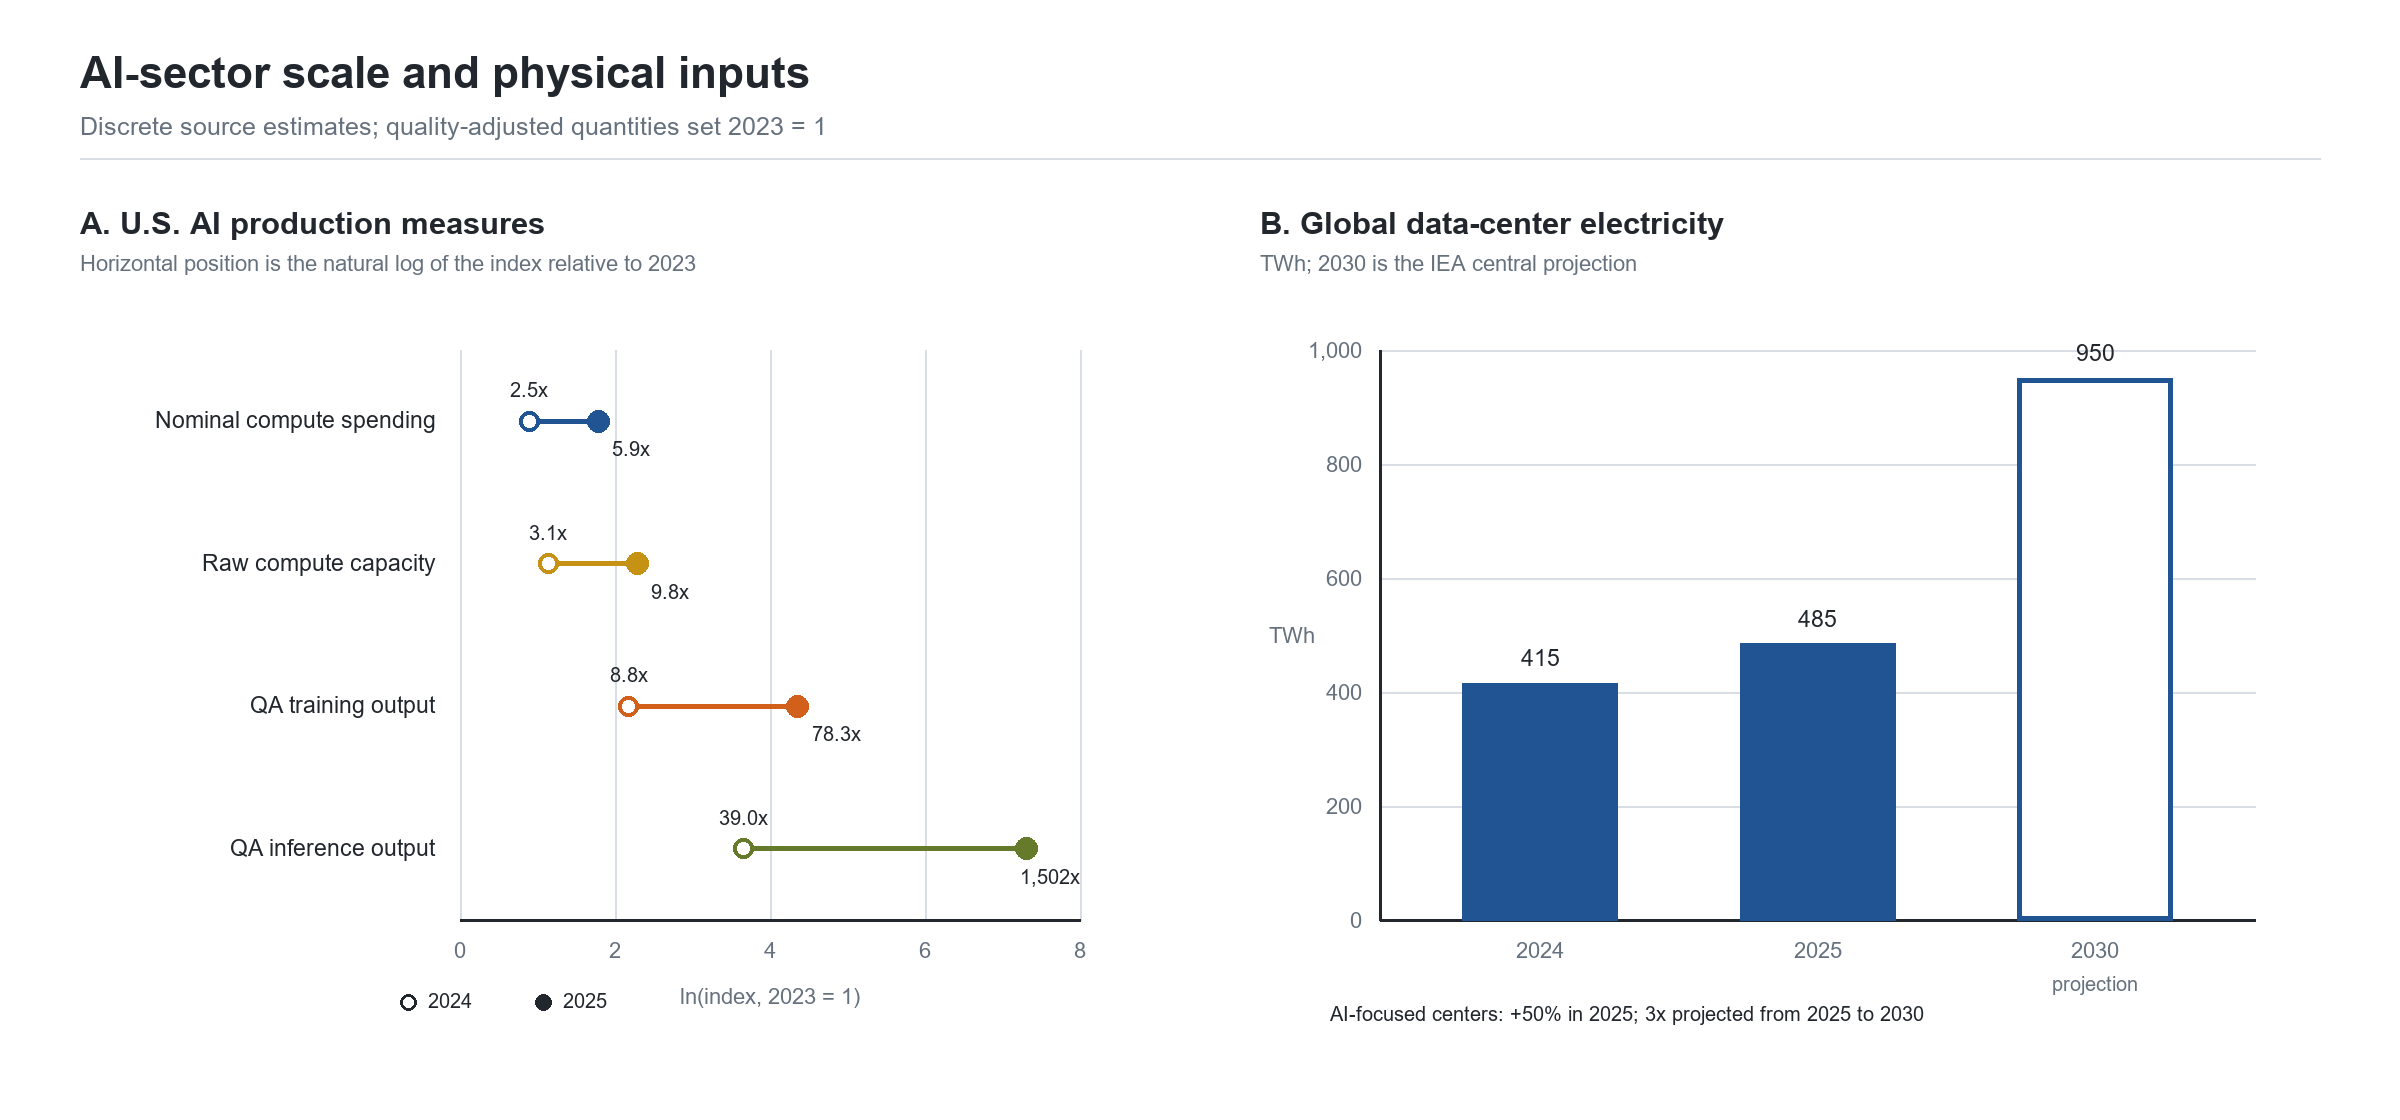
\includegraphics[width=\textwidth]{figures/empirical_ai_scale.png}
    \caption{AI-sector scale and physical inputs. Panel A reports discrete U.S.
    estimates for 2024 and 2025 relative to 2023; horizontal positions use the
    natural logarithm because the quality-adjusted quantities span several orders
    of magnitude. Panel B reports observed global data-center electricity use in
    2024 and 2025 and the IEA central projection for 2030. Sources:
    \citet{korinekmckelvey2026}, \citet{iea2025}, and \citet{iea2026}.}
    \label{fig:empirical-ai-scale}
\end{figure}

The cost of obtaining quality-adjusted AI services has fallen at the same time. The
lowest observed price for querying a model that reached the GPT-3.5 performance
level on MMLU fell from \$20 per million tokens in November 2022 to \$0.07 in October
2024. Over a similar period, the AI Index reports annual declines of 30 percent in
hardware costs and annual improvements of 40 percent in energy efficiency
\citep{stanfordaiindex2025}. This motivates our separation of raw inference compute
from quality-adjusted AI services. It does not identify AI capability separately: a
lower quality-adjusted price can reflect better algorithms, hardware, utilization,
or a lower markup.

Compute remains a real resource rather than a freely reproducible unit of
intelligence. Global electricity consumption by data centers rose from 415 TWh in
2024 to 485 TWh in 2025, while consumption at AI-focused facilities increased by 50
percent. The International Energy Agency projects total data-center consumption of
approximately 950 TWh in 2030 and a tripling of consumption at AI-focused facilities
between 2025 and 2030 \citep{iea2025,iea2026}. Figure
\ref{fig:empirical-ai-scale} therefore combines a rapid expansion in output with a
rapid, but much smaller, expansion in a physical input. This pattern motivates the
model's common resource cost and the compute and electricity constraints reserved
for the extended model. The baseline cost normalization is an abstraction, not a
claim that the marginal cost of compute will remain constant.

A different set of measurements speaks to capability and use. METR defines a
model's 50-percent task horizon as the length of task---measured by the time a human
expert would require---at which an AI agent succeeds half of the time. Its public
suite covers software engineering, machine learning, and cybersecurity tasks. The
estimated horizon rises sharply across model releases, but it is not the amount of
time an AI system works autonomously, and METR cautions that estimates above 16
hours are unreliable with the current task suite \citep{metrtimehorizon2026}.
Platform use provides another imperfect signal. In Anthropic's samples of Claude.ai
conversations, the share classified as directive---a subset of automation---was 27
percent in January 2025, 39 percent in August, and 32 percent in November
\citep{anthropiceconomicindex2025,anthropiceconomicindex2026}. The non-monotonic path
is itself useful: capability growth does not translate mechanically into realized
delegation. These proprietary samples cover one platform and conversations rather
than production quantities.

\begin{figure}[H]
    \centering
    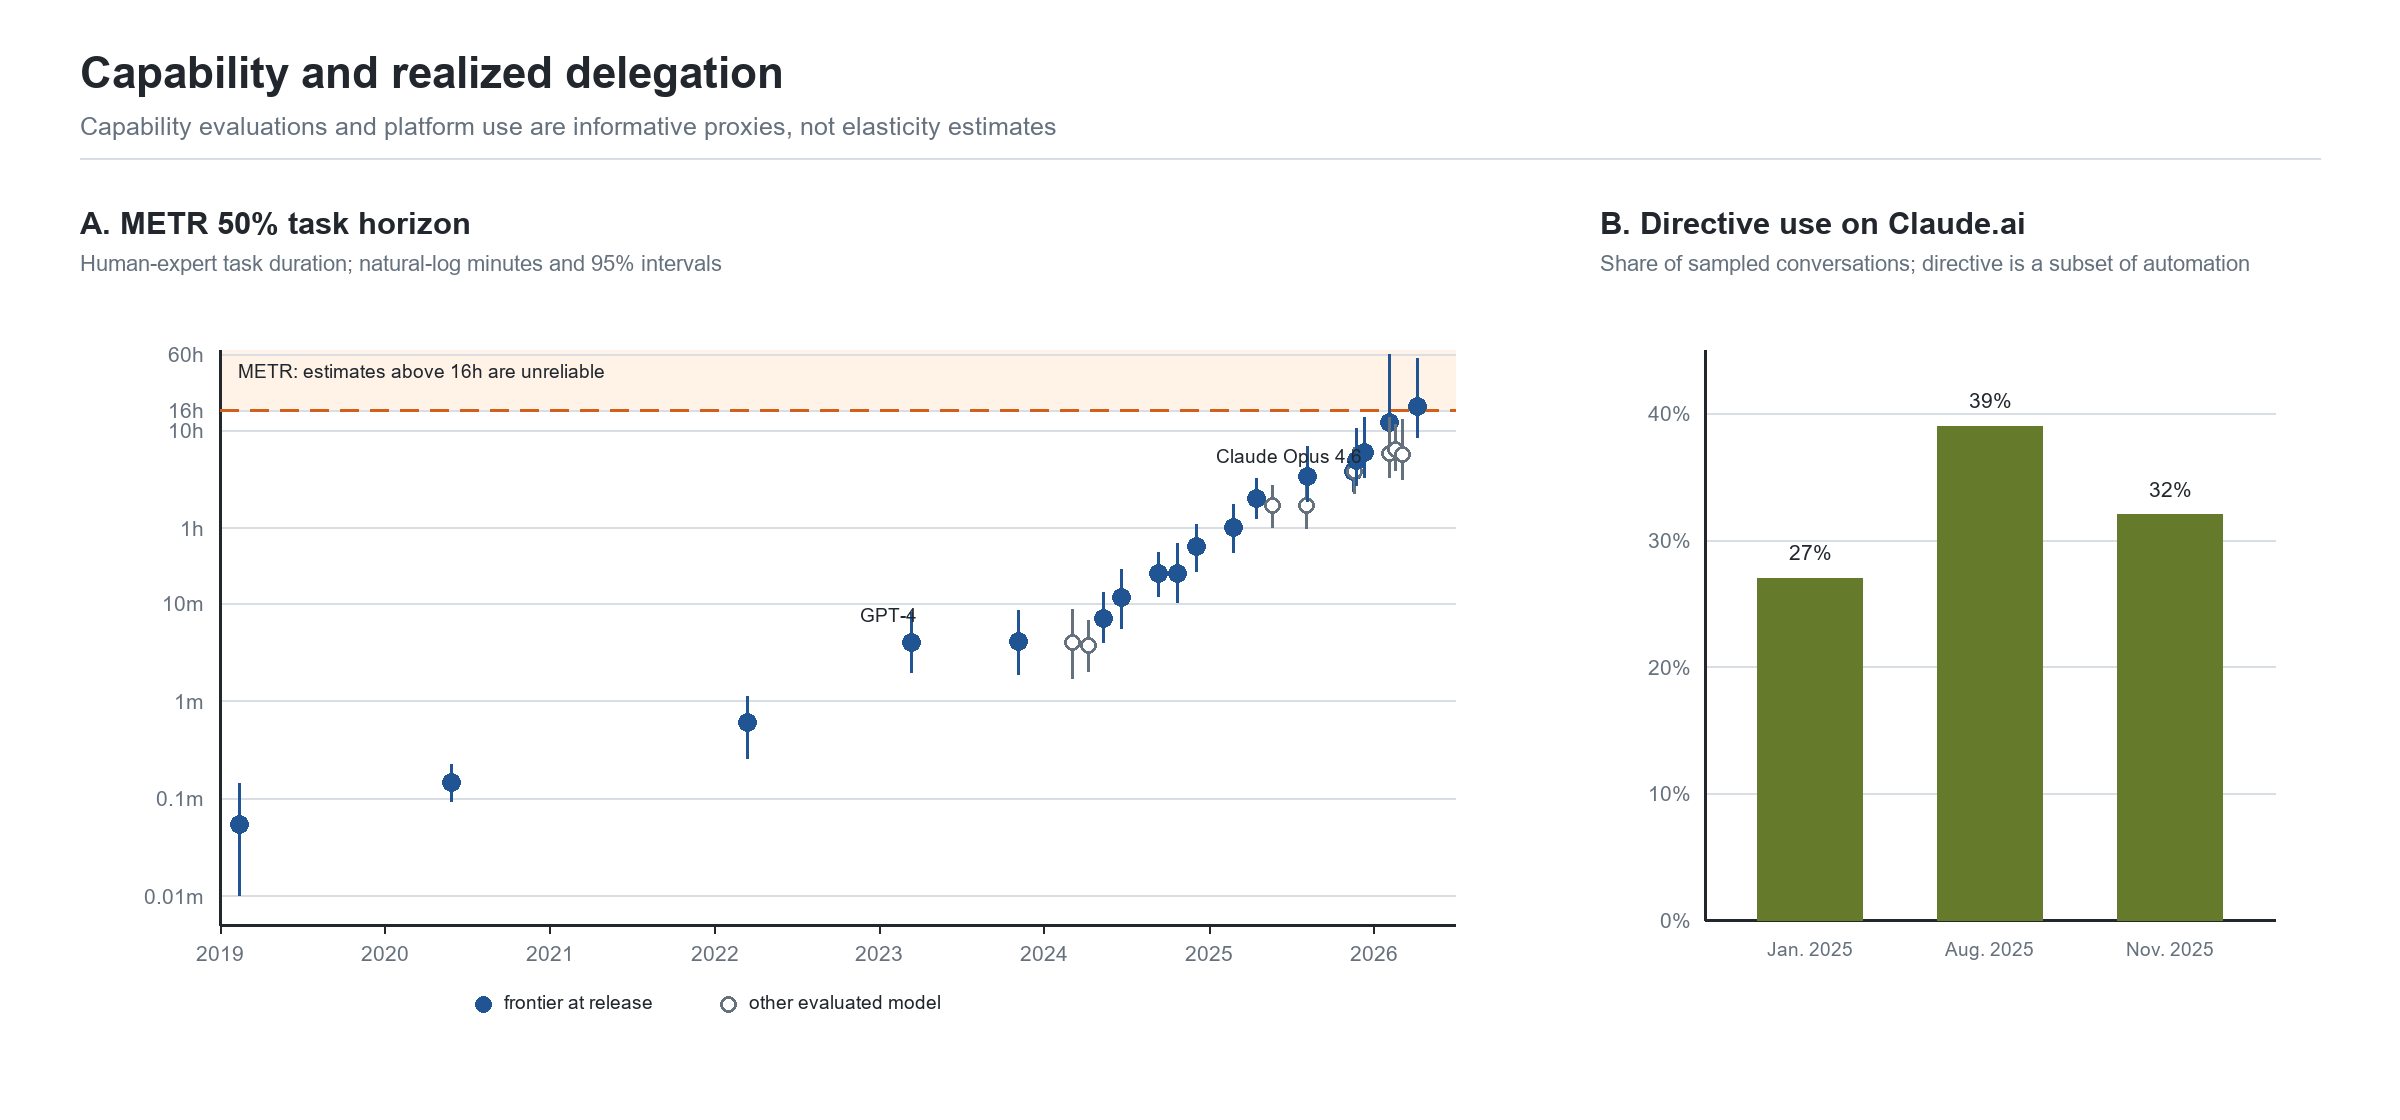
\includegraphics[width=\textwidth]{figures/empirical_automation_proxies.png}
    \caption{Capability and realized delegation. Panel A reports METR's estimated
    50-percent task horizon and 95-percent intervals for 26 evaluated models; the
    vertical scale is the natural logarithm of human-expert task minutes. The shaded
    region marks estimates above 16 hours, which METR regards as unreliable with the
    current task suite. Panel B reports directive use as a share of sampled Claude.ai
    conversations. Directive use is a subset of Anthropic's automation category.
    Sources: \citet{metrtimehorizon2026}, \citet{anthropiceconomicindex2025}, and
    \citet{anthropiceconomicindex2026}.}
    \label{fig:empirical-automation-proxies}
\end{figure}

Evidence closest to the automation of AI research comes from controlled evaluations,
not aggregate time series. In the original RE-Bench study, human experts given a
32-hour budget achieved almost twice the average score of the best AI agent on a set
of machine-learning research-engineering tasks \citep{metrrebench2024}. In a later
evaluation on a five-task subset, Claude 3.7 with a 32-hour budget matched the median
score of humans who had eight hours \citep{metrclaude2025}. This is evidence of a
changing frontier, but not a comparable two-date series: the model, scaffolding,
task subset, and time budgets differ. It therefore motivates the possibility that
automated research can substitute for human research without measuring the model's
human-to-machine research ratio.

Some striking internet statistics are less informative for our question. Cloudflare
reports that user-action crawler traffic rose by a factor of 21 during 2025 and that
AI bots accounted for an average of 4.2 percent of HTML page requests
\citep{cloudflareradar2025}. These are network requests, not tasks, workers, or value
added. We therefore do not treat bot traffic as evidence that AI has displaced human
labor.

Commercial scale has also increased. NVIDIA's data-center revenue rose from \$47.5
billion in fiscal year 2024 to \$115.2 billion in fiscal year 2025 and \$193.7
billion in fiscal year 2026 \citep{nvidia2026}. This is audited revenue from compute
hardware and networking, not total revenue from AI services. For frontier model
developers, the Stanford AI Index reports directional annualized-revenue estimates
of \$25 billion for OpenAI and \$19 billion for Anthropic around the beginning of
2026, while emphasizing differences in source quality and accounting definitions
\citep{stanfordaiindex2026}. The same report finds that industry produced more than
90 percent of notable models in 2025. These facts motivate a model in which private
demand, compute expenditure, and operating rents finance frontier research. They do
not establish monopoly or identify the markup earned by an integrated developer.

Taken together, the evidence motivates the model's state variables and the feedback
from AI services to AI research. It does not identify the substitution elasticity
between labor and AI services, the substitution elasticity between human and
automated research, or the probability of a singularity. We therefore do not use
these series to calibrate the transition. The numerical exercises discipline the
model's equilibrium logic; they are scenarios rather than forecasts.

\subsection{Economic mechanism and contribution}

This possibility raises an economic question before it raises a forecasting question.
Suppose frontier improvements combine human researchers and automated-research
services. Firms then choose both the scale and the composition of research. When the
research elasticity $\sigma_{HM}$ exceeds one, the two inputs are gross substitutes and
the automated share increases if the human research wage rises relative to the unit
resource cost of automated research. The conditional research-demand system
therefore represents automation as a continuous change in input composition rather
than as a date imposed on the model. Whether the equilibrium actually completes that
transition depends on the wage and automated-research-cost paths. Human researchers
can become asymptotically inessential, but substitution above one does not guarantee
that outcome: the wage must also rise relative to the cost of automated research.

Population growth is important during the human-dominated phase. In standard R\&D-based growth
models, new ideas depend on a growing but scarce human research input
\citep{romer1990,jones1995,aghionhowitt1992}. With diminishing returns to the stock of
ideas, a constant research-employment share implies semi-endogenous growth: the
long-run rate of innovation is pinned down by the growth of the research labor force.
Our benchmark preserves this logic while human research dominates. If population grows at rate
$n$, the capability growth rate is $\eta n/(1-\phi)$; without population growth,
positive asymptotic growth disappears when $\phi<1$.

Research automation can alter this result. Effective research labor can expand
through additional automated-research services rather than through population growth.
When those services dominate, capability growth is tied to their equilibrium growth
rate. Innovation can accelerate if higher output finances enough additional
automated research, but diminishing returns to ideas and research effort can preserve
a constant-growth path. The outcome depends separately on the production elasticity
$\sigma_{XL}$, the research elasticity $\sigma_{HM}$, and the allocation of output to research.

Human essentiality changes the strength of this feedback. Consider a counterfactual
in which research is Cobb--Douglas in human and automated inputs. Human research then
remains essential, and only the automated-input elasticity $\omega_M$ transmits the
feedback from output to research. Under Cobb--Douglas production, the human-essential
constant-growth candidate has a positive finite capability-growth rate only if
$1-\phi-\eta\omega_M\omega_X/\omega_L>0$. We maintain this restriction in the
baseline model and numerical experiments, but relax it in an analytical
counterfactual. Equivalently,
$\upsilon\equiv\beta/(1-\alpha-\beta)=\omega_X/\omega_L$. When automated research can instead become
asymptotically dominant, the condition becomes
$1-\phi-\eta\omega_X/\omega_L>0$. The second condition is stricter because $\omega_M<1$. There is
therefore a nonempty parameter region in which the human-essential candidate has
positive finite growth while the corresponding AI-dominated candidate does not.
Within the reduced proportional-allocation system, the sign of the human-essential
denominator also has an independent interpretation. A positive value produces a
stable positive growth rate, a zero value produces double-exponential capability,
and a negative value produces a finite-time singularity. The relevant threshold is
zero, not one.
This comparison is between two research technologies; it does not assume that the
research elasticity changes during the transition in the CES model. It is also
conditional on Cobb--Douglas production. If $\sigma_{XL}>1$ and capability is
unbounded, the output--capital ratio and the return to capital diverge. The household
Euler equation then makes consumption growth diverge, ruling out an interior steady
state with finite constant growth rates. This is a separate production-side
acceleration mechanism. Human essentiality weakens the research feedback but does
not by itself restore balanced growth.

The break at $\sigma_{XL}=1$ is asymptotic rather than a jump in finite allocations.
The exact CES share is continuous in the elasticity for every finite relative price,
but the limits in which $w/p^X$ becomes unbounded and the elasticity approaches one
do not commute. Under the high-capability regularity condition used below, unbounded
capability generates precisely this relative-price limit. Moreover, the relative-price threshold required for a given AI
share diverges exponentially in $1/(\sigma_{XL}-1)$. An elasticity just above one
can therefore produce an arbitrarily long quasi-Cobb--Douglas transition even though
its infinite-horizon regime has no finite constant-growth steady state.

The failure of the balanced-growth condition is not sufficient for a finite-time
singularity. Under the proportional-allocation closure used to isolate the feedback,
$D>0$ gives stable balanced growth, $D=0$ gives accelerating growth that remains
finite at every finite date, and a persistent $D<0$ produces a finite-time
singularity. During the CES transition, the relevant denominator is
$D(s^M_t)=1-\phi-\eta\upsilon s^M_t$. The automation share must cross the critical
value $(1-\phi)/(\eta\upsilon)$ and remain high long enough for the integral
condition derived below to be met. This distinction prevents the absence of a constant-growth path
from being interpreted mechanically as an immediate explosion.

Recent discussions often move too quickly from this mechanism to one of two
conclusions. One view treats an intelligence explosion as the natural implication of
automating AI research. The other assumes that physical bottlenecks and diminishing
returns will necessarily preserve familiar growth rates. Neither conclusion follows
without specifying the ideas production function. Scenario exercises such as
\citet{kokotajlo2025} make the feedback mechanism concrete, but rapid takeoff depends
on several jointly necessary assumptions about research automation, algorithmic
progress, compute, and organizational capacity. An economic model should expose those
assumptions separately.

Market structure determines both current use and the private return to innovation.
Frontier AI requires large fixed investments and may exhibit economies of scale and
scope \citep{korinekvipra2025,gans2024}. A monopolist restricts the current supply of
AI services but captures operating rents that raise the private value of better
capability. We therefore begin with one integrated developer that both supplies
quality-adjusted AI services and invests in the frontier. Competitive final-good
firms combine capital with a CES composite of production labor and AI services. The
production elasticity $\sigma_{XL}$ inside this composite governs adoption and the demand
elasticity faced by the monopolist.

The production elasticity $\sigma_{XL}$ separates the response of the real wage from the
response of the production-labor share. An expansion of AI services reduces this share when AI and
production labor are gross substitutes, but the wage falls only when substitution is
sufficiently strong. There is therefore an intermediate region in which production
workers receive a smaller share of output even though their wage rises. This
distinction is important for the distributional analysis: a declining labor share is
not, by itself, evidence that the real wage has fallen. In the full model, the
aggregate labor share also depends on how workers are reallocated between production
and research. An increase in the human-research employment share raises aggregate
labor income relative to production labor income; a decrease lowers it.
There is a sharper conditional result under Cobb--Douglas research and a fixed
automated-research spending share. The human-research wage bill is then a constant
share of output, so the production and aggregate labor-income shares rise together
when $\sigma_{XL}<1$ and remain constant when $\sigma_{XL}=1$. This result belongs
to a reduced allocation rule and is not used to characterize the numerical
equilibrium paths.

A separate distinction operates within the AI-development industry. The ratio
$H/M$ measures the human intensity of research, whereas $H/N$ measures the fraction
of the population employed as human researchers. Research can become less human
intensive while the development industry employs more people: $H/M$ falls when
automated research becomes cheaper relative to human research, but $H/N$ rises if
the scale of automated research per capita expands sufficiently quickly. The model
therefore allows an initial decline followed by an increase in human research
employment even along a path of continuous research automation.

The resulting welfare problem has two distinct margins. Static market power reduces
the current use of AI services. At the same time, consumer surplus and knowledge
spillovers imply that the developer may capture only part of the social value of
better AI and therefore invest too little in research. Reducing the markup can
correct the deployment distortion while also eroding the rents that finance
innovation. Price regulation and research policy must consequently be studied
together. The present version isolates this market-structure mechanism.

The six technology classes defined by $\sigma_{HM}\in\{1,>1\}$ and
$\sigma_{XL}\in\{<1,1,>1\}$ organize four groups of results. First, research automation is a
continuous equilibrium transition. Its speed depends on $\sigma_{HM}$ and on the
growth of the human research wage relative to the cost of automated research;
$\sigma_{HM}>1$ alone does not make the human contribution disappear. The same
conditions distinguish research composition from research employment: $H/M$ can
fall while $H/N$ rises.

Second, the model characterizes the feedback from research automation to growth.
Population growth sustains semi-endogenous capability growth while human research
dominates. If human and automated research are Cobb--Douglas, the essential human
input weakens the feedback from output to innovation. When automated research can
instead become asymptotically dominant, the stability condition is strictly more
demanding. The two candidate allocations identify a parameter region in which the
human-essential candidate has positive finite growth but the AI-dominated candidate
does not. Under
the reduced proportional-allocation closure, a positive value of the feedback denominator gives
constant growth, a zero denominator gives acceleration without finite-time
divergence, and a sufficiently persistent negative denominator gives a finite-time
singularity. With an endogenous automation share, a temporary crossing of the local
threshold is not sufficient; the accumulated feedback must reach the exact integral
condition derived below.
The fully Cobb--Douglas counterfactual makes the distinction especially transparent.
Even with unit substitution elasticities in production and research, an exact balance
between diminishing returns and the output--research feedback makes the capability
growth rate rise without bound. If the feedback is stronger, the reduced system
reaches a finite-time singularity. Explosive growth therefore does not require
$\sigma_{XL}>1$.

Third, the production elasticity creates a separate phase diagram. If
$\sigma_{XL}<1$, labor remains a bottleneck and any interior constant-growth limit
has zero per-capita output growth. In any nondegenerate limit that also satisfies the
developer's optimality conditions, human and automated research grow more slowly
than population and capability grows at rate $\eta n/(1-\phi+\eta)$. At
$\sigma_{XL}=1$, an AI-dominated positive constant-growth candidate requires the
stability and resource-feasibility restrictions. If
$\sigma_{XL}>1$ and capability is unbounded, the output--capital ratio and the return
to capital diverge, so the household Euler equation rules out an interior steady
state with finite constant growth rates. This remains true when human research is
essential. The discontinuity at one is a singular perturbation: finite allocations
are continuous in $\sigma_{XL}$, but the asymptotic limits do not commute and the
scale required for AI dominance diverges as $\sigma_{XL}\downarrow1$.

Fourth, the production structure separates factor-income outcomes. An expansion of
AI services lowers production labor's share when $\sigma_{XL}>1$, whereas its direct
effect raises the real wage when $\sigma_{XL}<1/\alpha$. Capital deepening and the
reallocation of workers between production and research determine the corresponding
general-equilibrium paths. The exact wage-growth decomposition identifies when
AI-services deepening works against wage growth, but the paper does not claim that
this force dominates without solving the associated equilibrium transition. The
aggregate labor share can also differ from the production-labor share because it
includes human researchers. Finally, monopoly creates a static deployment
distortion but also the rents that give frontier capability a private value; an
explicit social-value extension can create a distinct reason for private research to
remain below the social level. The baseline model does not sign that wedge.

The numerical section solves the decentralized perfect-foresight canonical system,
rather than fixing investment and research-spending shares. Under
$\sigma_{XL}=0.75$, output per capita falls initially, recovers, and then converges
toward a constant level while capability continues to grow. The production-labor
share rises as labor becomes the bottleneck. Under Cobb--Douglas production,
research automation is gradual: the automated contribution to research rises from
10.6 percent initially to 45.4 percent after 600 years and approaches one only over
a much longer horizon. Capability and per-capita output growth converge to their
analytical constant-growth values. Human research employment is non-monotone along
this path even though its long-run share of the population is zero.

A second Cobb--Douglas production path changes only the research elasticity from
$\sigma_{HM}=2$ to $\sigma_{HM}=1$. Human research then remains essential and its
share of the population converges to 0.497 percent. Capability growth converges to
1.738 percent rather than 2.274 percent, and per-capita output growth converges to
0.435 percent rather than 0.568 percent. Both paths satisfy the same canonical
equilibrium system. The comparison isolates how research substitutability changes
both the composition of research and the strength of recursive feedback.

For $\sigma_{XL}>1$, the numerical section uses the model's singular asymptotic
ratios rather than imposing a nonexistent finite-growth terminal state. Calendar
time to a large output--capital ratio is endogenous, and the boundary is moved
outward until the initial jump variables and the implied singularity date converge.
The common parameters keep both the human-essential and AI-dominated research
feedback denominators positive. The high-$\sigma_{XL}$ experiments therefore isolate
the production-side acceleration mechanism rather than the $D_{\mathrm{CD}}\leq0$
counterfactual.
For $\sigma_{XL}=1.35$, 1.50, and 2.00, the selected equilibrium branch remains close to moderate
growth for a long interval and then accelerates toward a finite-time singularity.
Higher substitution brings the acceleration forward. The wage rises throughout
all three paths, while the aggregate labor share approaches zero. These dates are
conditional numerical examples, not calibrated forecasts.

An additional search crosses the static wage threshold $1/\alpha$ and jointly
considers high production elasticities and faster population growth. These paths
satisfy the canonical equilibrium equations on their computed domains, but they
extrapolate the AI-dominated terminal boundary beyond the region established by the
analytical result. The computed wage can fall temporarily: with
$\sigma_{XL}=6.28$ and $n=3.9$ percent, its peak-to-trough decline is 9.39 percent.
The wage then recovers as capital accumulates and the movement of workers into AI
research makes production labor scarce. The wage at the trough remains 16.72 percent
above its initial level. This is a conditional numerical branch, not a proof that
every equilibrium with a high production elasticity eventually recovers.

Figure~\ref{fig:high-sigma-equilibrium-growth} previews this transition. It is
included here to show the quantitative object the paper seeks to explain, not as
evidence for the propositions. Section~\ref{sec:analytical-results} derives the
analytical foundations used across regimes. Section~\ref{sec:numerical} then
organizes the results into four cases and presents, within each case, the analytical
characterization and an equilibrium transition.

\begin{figure}[htbp]
    \centering
    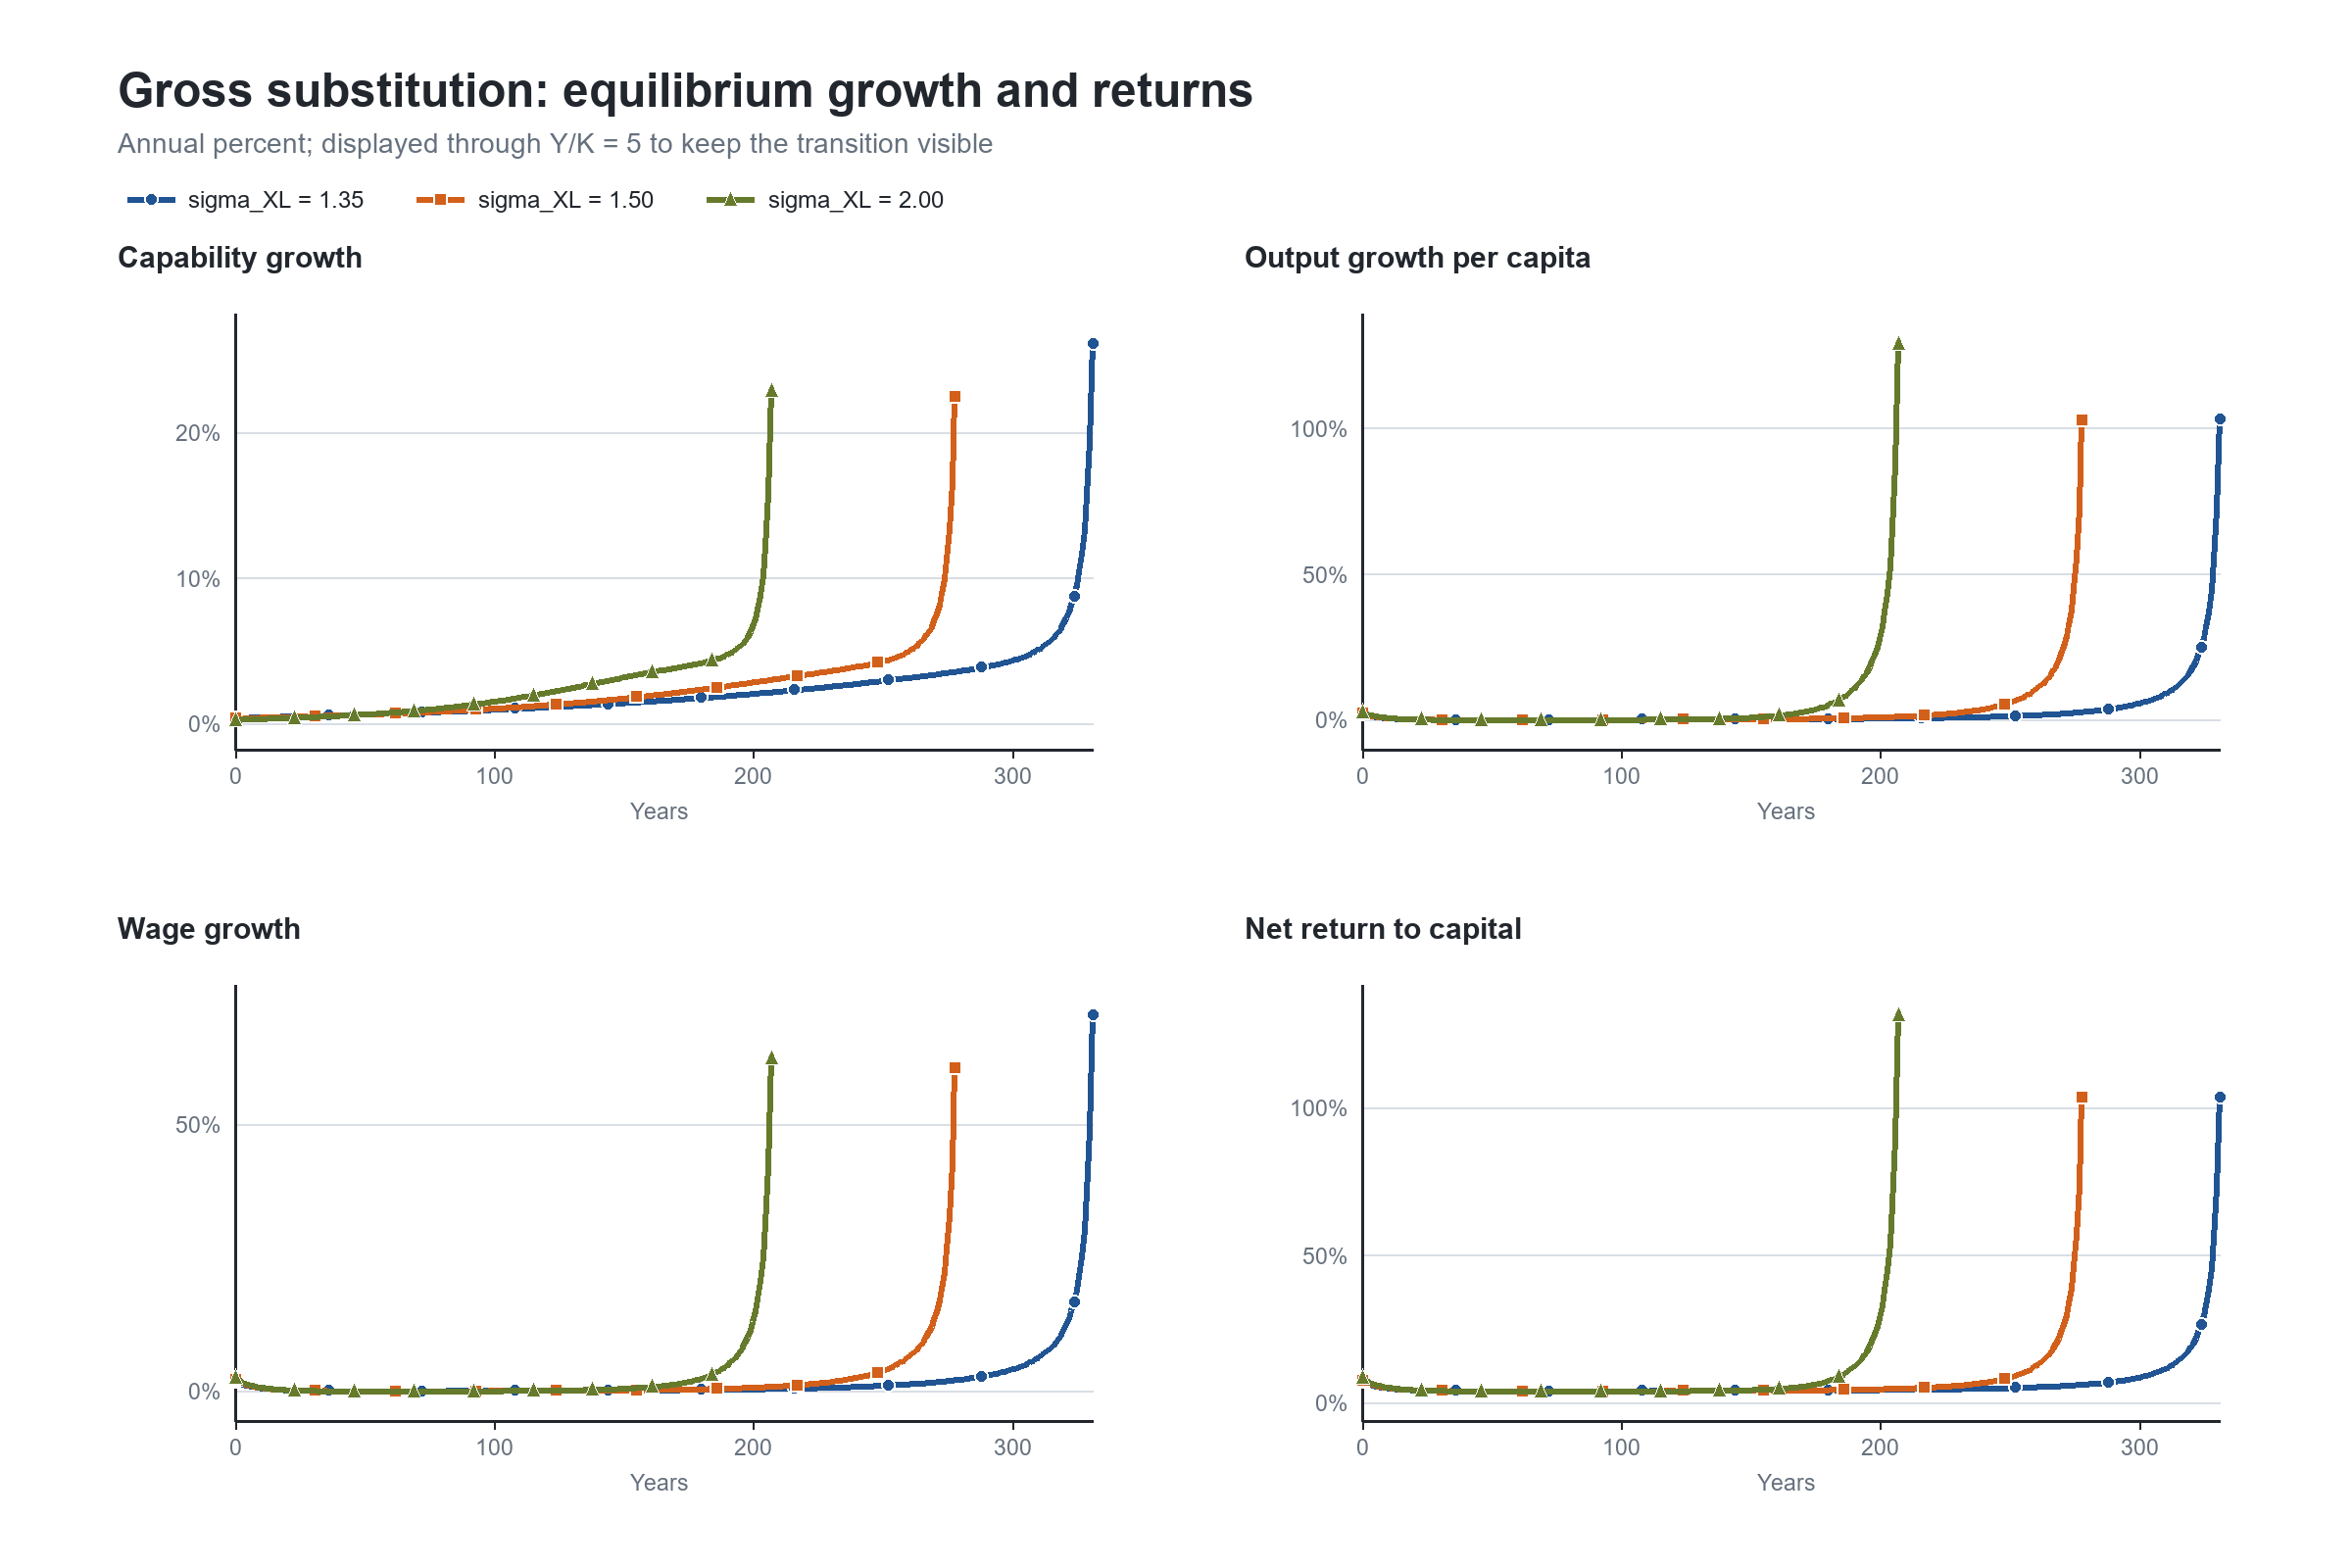
\includegraphics[width=\textwidth]{figures/high_sigma_equilibrium_growth.png}
    \caption{Preview of equilibrium growth rates and the net return under gross
    substitution. The figure stops at $Y/K=5$ to keep the pre-acceleration
    transition visible. The paths and their numerical validation are presented in
    Section~\ref{sec:numerical}.}
    \label{fig:high-sigma-equilibrium-growth}
\end{figure}

The extended model retains the integrated monopolist and adds distributional
heterogeneity and richer capital and compute accumulation. It will compare a
laissez-faire monopoly with regulated access prices, research subsidies or prizes,
and policies that combine both instruments. The objective is not to select a policy
before solving the model. It is to identify when lower AI-service prices must be
paired with explicit support for frontier research.

A task-based extension introduces task-specific AI productivity and fixed
automation costs. The extension makes the set of automated research tasks
endogenous and separates the intensive human--machine substitution margin from the
extensive margin on which new tasks become economical to automate. It also provides
a second reason for an initially small automated share: at low research scale, the
variable-cost savings from automation may not cover task-specific integration and
verification costs.

The rest of the paper is organized as follows. Section~\ref{sec:literature} relates
the framework to endogenous growth, transformative AI, automation and labor income,
measurement of AI services, and industrial organization. Section~\ref{sec:toy}
develops the baseline model and derives the analytical foundations.
Section~\ref{sec:numerical} studies four growth regimes. Each regime pairs the
relevant analytical result with an audited numerical equilibrium path.
Section~\ref{sec:extended} sets out the extended general-equilibrium model, and
Section~\ref{sec:task-extension} introduces research tasks and fixed automation
costs.
Section~\ref{sec:regulation} defines the regulatory scenarios.
Section~\ref{sec:conclusion} concludes.

\section{Related literature}
\label{sec:literature}

The paper connects five literatures that are usually studied separately.

\paragraph{Endogenous innovation and economic growth.}
The first literature makes ideas production an economic activity. In
\citet{romer1990}, nonrival knowledge and imperfect competition sustain investment in
new varieties. \citet{aghionhowitt1992} model growth through quality-improving creative
destruction. \citet{jones1995} shows that diminishing returns in the production of ideas
remove scale effects and tie long-run growth to the growth of the research labor force.
Our starting point is closest to the semi-endogenous formulation: human researchers
are initially the scarce input that limits innovation. The departure is that research
labor can itself be produced with AI and compute.

\paragraph{Capital substitution and asymptotically linear growth.}
The capital-deepening benchmark belongs to a different growth tradition.
\citet{solow1956} and \citet{pitchford1960} show that a sufficiently high elasticity
of substitution can keep the marginal product of capital from vanishing in a model
with a constant saving rate. \citet{jonesmanuelli1990} characterize the broader class
of convex technologies that become asymptotically linear, and \citet{rebelo1991}
shows how an accumulable capital core can sustain endogenous growth without
increasing returns. \citet{duffypapageorgiou2000} emphasize the qualification that an
elasticity above one is necessary but not sufficient: asymptotic capital productivity
must also exceed the depreciation and population-growth requirement. Our benchmark
uses two capital services to make this comparison transparent. Its nested architecture
is close to \citet{kruselletral2000}, who combine structures capital in an outer
Cobb--Douglas layer with equipment capital and labor inputs inside a CES nest. Unlike
their quantitative model, our benchmark fixes the division of total capital and uses
it only to separate ordinary capital deepening from recursive improvement in AI
capability.

\paragraph{AI, automation, and the production of ideas.}
\citet{aghionjonesjones2019} examine AI as an automation technology and emphasize that
growth can remain constrained by tasks that are essential but difficult to automate.
\citet{acemoglu2025} also models AI at the task level and relates its aggregate
productivity effect to the share of tasks affected and the cost savings within those
tasks.
\citet{nordhaus2021} studies the substitutability conditions required for an economic
singularity. \citet{trammellkorinek2023} distinguish the automation of ordinary
production from the automation of R\&D and show that physical and technological
bottlenecks remain central even under transformative AI. \citet{jones2025rd} provides
a general framework in which AI's effect on research depends on the share of tasks it
can perform, its productivity in those tasks, and the strength of complementary
bottlenecks. Our model endogenizes the gradual composition of human and automated
research and embeds the ideas production function in a decentralized market
equilibrium.

\paragraph{Automation, wages, and the labor share.}
The effect of automation on labor income depends on both substitution and
productivity. \citet{acemoglurestrepo2019} distinguish the displacement effect of
automating existing tasks from the productivity and reinstatement effects that can
raise labor demand. In CES models, the unit-elasticity threshold determines whether
an increase in a factor reduces the income share of the other factor. This mechanism
underlies the account in \citet{karabarbounisneiman2014} of how cheaper investment
goods can reduce the labor share. A lower labor share, however, does not imply a lower
real wage. Using a nested CES and Korean firm and establishment data,
\citet{aumshin2024} estimate an elasticity of 0.6 between equipment and labor and an
elasticity of 1.6 between software and labor. The second estimate is a useful
empirical reference for our production elasticity $\sigma_{XL}$ because $X$ is a flow of
AI services rather than a stock of conventional equipment. It is not a direct
estimate of substitution between AI services and labor in the world economy.
\citet{autorkausik2026} establish more generally that automation can raise
wages while reducing labor's share in a competitive constant-returns economy.
\citet{yango2026} obtains, in a nested Cobb--Douglas--CES technology, the same two
thresholds that appear in our production block: the labor share falls when
$\sigma_{XL}>1$, while the wage rises when $\sigma_{XL}<1/\alpha$. Thus, for
$1<\sigma_{XL}<1/\alpha$, an expansion of AI simultaneously raises the wage and lowers
labor's share of income. \citet{trammellkorinek2023} place this ambiguity in the
broader transformative-AI literature: production automation can sharply reduce the
labor share, while the wage response continues to depend on technology and
accumulation.

We use the two-threshold result as a benchmark rather than claim it as a new
comparative static. Our departure is to make AI a flow of quality-adjusted services
supplied by an integrated monopolist and to make the underlying capability frontier
endogenous. Market power changes the equilibrium path of AI deployment, capital
accumulation, wages, and operating rents; frontier research determines how long the
economy remains in each production regime. This structure lets us study how service
regulation and research policy affect the wage and the labor share through different
static and dynamic channels.

\paragraph{AI services, inference compute, and quality adjustment.}
Using an existing model and producing a new one require separate measures of
inference and research compute. \citet{korinekmckelvey2026} combine inference compute
with intangible model capital and adjust the resulting output for quality.
\citet{demireretal2025} document prices per token within intelligence tiers, which
likewise implies that raw tokens are not homogeneous AI services. Our specification
$X_t=A_tU_t$ is an efficiency-units representation, not a technological identity:
$U_t$ measures the scale at which the current model is run, while $A_t$ converts
inference compute into quality-adjusted services. Task-based formulations such as
\citet{aghionjonesjones2019} and \citet{acemoglu2025} provide a richer alternative
when heterogeneity across uses of AI is central.

\paragraph{Market structure in AI.}
The industrial-organization literature emphasizes high fixed costs, scarce compute,
data, economies of scope, vertical integration, and feedback between model quality and
the surrounding ecosystem. \citet{korinekvipra2025} study how these forces can produce
concentration and tipping in foundation models. \citet{gans2024} emphasizes the role of
markets for training and input data in determining market power. Using model-usage
data, \citet{demireretal2025} document entry, falling prices, differentiation, and
turnover among leading models. The evidence is consistent with strong competition
today but does not rule out future concentration. Our extended model focuses on a
specific dynamic mechanism: a temporary lead becomes persistent when it lowers the
leader's cost of producing the next generation of frontier models.

Our baseline takes this concentration to its limiting case: one integrated frontier
developer supplies current services and conducts frontier research. Regulated access
prices are introduced as policy counterfactuals rather than as a second baseline
market structure. This formulation isolates the dynamic link between current
operating rents and the private incentive to improve the frontier.

\paragraph{Contribution relative to existing work.}
Several individual mechanisms in the model are established in the literature and
are not claimed as new. Semi-endogenous growth already ties long-run innovation to
population growth when human research labor is the expanding input. The possibility
of an economic singularity, the importance of essential tasks, and the distinction
between automating production and automating R\&D are central to
\citet{aghionjonesjones2019}, \citet{nordhaus2021}, and
\citet{trammellkorinek2023}. The two static thresholds separating the real wage from
labor's income share appear in recent automation models, including
\citet{autorkausik2026} and \citet{yango2026}. Nor is the general trade-off between
market power and innovation new. The paper uses these results as building blocks.

The first departure is to make the composition of AI research a continuous
equilibrium object inside a dynamic macroeconomic model. Relative to the task-based
research framework in \citet{jones2025rd}, the baseline suppresses heterogeneity
across research tasks but endogenizes the aggregate automation share through the
relative price of human and automated research. That share then enters the feedback
denominator governing capability growth. The task extension restores an extensive
automation margin while preserving the connection to the decentralized equilibrium.

The second departure is the formal comparison between human-essential and
AI-dominated research. With Cobb--Douglas production, the two feedback denominators
are
\[
    D_{\mathrm{CD}}
    =1-\phi-\eta\omega_M\frac{\omega_X}{\omega_L},
    \qquad
    D_{\mathrm{AI}}
    =1-\phi-\eta\frac{\omega_X}{\omega_L}.
\]
Their difference identifies a parameter region in which the human-essential
constant-growth candidate has a positive finite rate but the AI-dominated candidate
does not. In the reduced proportional-allocation system, the changing CES research
share also yields an exact path condition for finite-time singularity. That condition
characterizes the reduced system; it is not an existence theorem for the fully
optimizing equilibrium.
The fully Cobb--Douglas counterfactual also connects the paper to the recursive-growth
mechanism in \citet{aghionjonesjones2019}. Within the reduced system, at unit
substitution elasticities in both nests, the sign of $D_{\mathrm{CD}}$ alone
separates a stable positive growth rate,
double-exponential capability, and a finite-time singularity. Gross substitution in
final production is therefore one route to acceleration, not a necessary condition
for it.

The third departure concerns the interaction between recursive innovation and the
production CES. The paper proves that, for every fixed $\sigma_{XL}>1$, an interior
steady state with positive constant capability growth cannot exist: such a path would
make capability and the return to capital diverge, contradicting the household Euler
equation. It also shows that the unit-elasticity boundary is
a singular perturbation: finite allocations are continuous in $\sigma_{XL}$, while
the infinite-horizon limits do not commute and the scale required for AI dominance
diverges as the elasticity approaches one. This result complements the broader phase
diagrams in \citet{nordhaus2021} and \citet{trammellkorinek2023} by deriving the
transition in an economy with quality-adjusted AI services, capital accumulation,
and monopoly pricing.

The fourth departure is to connect research composition, research employment, and
market structure. The ratio $H/M$ can fall while $H/N$ rises because automation
changes the human intensity of research and the scale of the research industry at
the same time. The integrated developer links those employment dynamics to current
AI-service rents and frontier investment. This combination differs from the
market-structure analyses in \citet{gans2024} and \citet{korinekvipra2025}, which explain
the sources of concentration but do not embed the service provider's research choice
in the same aggregate transition system. We therefore describe the contribution as
the joint equilibrium characterization of these mechanisms rather than claim
priority for each ingredient separately.

\section{Baseline model and analytical foundations}
\label{sec:toy}

The toy model isolates the interaction between population growth, market power in
current AI services, and the automation of AI research. Time is continuous. There is
one final good, a representative dynasty, competitive final-good firms, and one
integrated frontier developer. The developer monopolistically supplies AI services
and invests in the next generation of AI. The initial economy already uses AI
services in production; the model does not describe their first commercial adoption.

The model contains four linked blocks: labor allocation, current production, frontier
research, and goods allocation. The diagrams below present each block where its
equations are introduced. Variables repeated across diagrams connect the blocks.
Solid arrows denote within-period production or resource use; dashed arrows denote
state accumulation. This separation is important because the model is a dynamic
system with feedback, not a one-way production tree.

\tikzset{
    model-input/.style={draw, rounded corners=2pt, minimum width=2.7cm,
        minimum height=1.0cm, align=center, fill=gray!8},
    model-state/.style={draw, rounded corners=2pt, minimum width=2.7cm,
        minimum height=1.0cm, align=center, fill=blue!8},
    model-technology/.style={draw, rounded corners=2pt, minimum width=3.5cm,
        minimum height=1.0cm, align=center, fill=orange!9},
    model-allocation/.style={draw, rounded corners=2pt, minimum width=3.5cm,
        minimum height=1.0cm, align=center, fill=gray!8},
    model-flow/.style={->, semithick},
    model-dynamics/.style={->, semithick, dashed}
}

\subsection{Household}

Population grows at the exogenous rate $n$:
\begin{equation}
    \dot N_t=nN_t,
    \qquad N_0>0,\quad n\geq0.
    \label{eq:population}
\end{equation}
The representative dynasty has preferences
\begin{equation}
    \int_0^\infty e^{-\rho t}N_t\log c_t\dd t,
    \qquad
    c_t\equiv\frac{C_t}{N_t},
    \qquad \rho>n,
    \label{eq:utility}
\end{equation}
where $C_t$ is aggregate consumption. Each household member supplies one unit of
labor inelastically. Labor is allocated between final production, $L_t$, and
human AI research, $H_t$:
\begin{equation}
    L_t+H_t=N_t.
    \label{eq:labor-clearing}
\end{equation}
Figure~\ref{fig:labor-allocation-flow} shows the associated opportunity cost. An
additional worker assigned to AI research reduces the labor available for current
production.

\begin{figure}[H]
    \centering
    \begin{tikzpicture}[>=Latex,font=\small]
        \node[model-state]      (N)     at (-3.8, 0.0) {$N_t$\\population};
        \node[model-allocation] (labor) at ( 0.0, 0.0)
            {$N_t=L_t+H_t$\\labor allocation};
        \node[model-input]      (L)     at ( 3.8, 1.1) {$L_t$\\production labor};
        \node[model-input]      (H)     at ( 3.8,-1.1) {$H_t$\\human research};

        \draw[model-flow] (N) -- (labor);
        \draw[model-flow] (labor) -- (L);
        \draw[model-flow] (labor) -- (H);
    \end{tikzpicture}
    \caption{Allocation of population between current production and human AI
    research.}
    \label{fig:labor-allocation-flow}
\end{figure}

The dynasty owns the capital stock and the frontier developer. Capital evolves as
\begin{equation}
    \dot K_t=I_t-\delta K_t.
    \label{eq:capital-law}
\end{equation}
Let $k_t\equiv K_t/N_t$. The per-capita budget constraint is
\begin{equation}
    \dot k_t
    =
    (r_t-\delta-n)k_t+w_t
    +\frac{\pi^X_t-w_tH_t-\xi M_t}{N_t}
    -c_t,
    \label{eq:household-budget}
\end{equation}
where $\pi^X_t$ is the developer's operating profit before research expenditure.
The household's Euler equation is
\begin{equation}
    \frac{\dot c_t}{c_t}=r_t-\delta-\rho.
    \label{eq:euler}
\end{equation}

\subsection{Final-good firms}

Competitive final-good firms combine physical capital with a composite of production
labor and AI services:
\begin{align}
    Y_t
    &=
    K_t^\alpha Z_t^{1-\alpha},
    \qquad \alpha\in(0,1),
    \label{eq:final-production}\\
    Z_t
    &=
    \left[
        \omega_L L_t^{(\sigma_{XL}-1)/\sigma_{XL}}
        +\omega_X X_t^{(\sigma_{XL}-1)/\sigma_{XL}}
    \right]^{\sigma_{XL}/(\sigma_{XL}-1)}.
    \label{eq:service-composite}
\end{align}
The elasticity of substitution between capital and the service composite is one.
The elasticity between production labor and AI services is $\sigma_{XL}$. The
Cobb--Douglas composite is obtained by continuity when $\sigma_{XL}=1$. We assume
$\sigma_{XL}>0$. The pair $(\omega_L,\omega_X)$ contains positive CES distribution
weights satisfying $\omega_L+\omega_X=1$, not generally observed factor-income
shares; the latter are endogenous and vary with relative quantities when
$\sigma_{XL}\neq1$.

Define the contribution of AI services to the CES composite as
\begin{equation}
    s^X_t
    \equiv
    \frac{\omega_X X_t^{(\sigma_{XL}-1)/\sigma_{XL}}}
    {\omega_L L_t^{(\sigma_{XL}-1)/\sigma_{XL}}
        +\omega_X X_t^{(\sigma_{XL}-1)/\sigma_{XL}}}.
    \label{eq:ai-composite-share}
\end{equation}
Let $p^X_t$ denote the price of AI services. Profit maximization gives
\begin{align}
    r_t
    &=\alpha\frac{Y_t}{K_t},
    \label{eq:capital-demand}\\
    w_t
    &=(1-\alpha)(1-s^X_t)\frac{Y_t}{L_t},
    \label{eq:labor-demand}\\
    p^X_t
    &=(1-\alpha)s^X_t\frac{Y_t}{X_t},
    \label{eq:ai-demand}
\end{align}
and relative demand satisfies
\begin{equation}
    \frac{X_t}{L_t}
    =
    \left[
        \frac{\omega_X}{\omega_L}
        \frac{w_t}{p^X_t}
    \right]^{\sigma_{XL}}.
    \label{eq:relative-ai-demand}
\end{equation}

\subsection{Integrated AI monopolist}

The variable $U_t$ is a flow of \emph{inference compute}: standardized
computational resources used during period $t$ to run an existing model. It can be
measured in FLOPs, GPU-hours, or equivalent units of a reference processor per unit
of time; it is not a stock of chips. Let $\xi>0$ denote the common unit resource cost
of standardized compute. It summarizes the capital, energy, and other resources
needed to supply one unit of compute, independently of whether that unit is used for
inference or research.

The variable $X_t$ is a flow of quality-adjusted AI services used by final-good
firms. Its empirical counterpart could be benchmark-equivalent tokens, predictions
adjusted for accuracy, or equivalent task hours. This distinction follows the
measurement approach in \citet{korinekmckelvey2026}, who combine inference compute
with model capital and adjust inference output for quality, and is consistent with
the intelligence tiers documented by \citet{demireretal2025}.

The stock $A_t$ measures frontier AI capability. Under the normalization used here,
it also measures quality-adjusted services produced per unit of inference compute:
\begin{equation}
    X_t=A_tU_t.
    \label{eq:ai-services}
\end{equation}
Equation~\eqref{eq:ai-services} is an efficiency-units specification, not a
technological identity. Conditional on $A_t$, it imposes constant returns to
inference compute and compresses task coverage, quality, speed, and inference
efficiency into one scalar.

Figure~\ref{fig:current-production-flow} combines the AI-service technology with the
two nests used by final-good firms. It therefore shows how capability and inference
compute affect current output, holding research and goods allocation outside the
diagram.

\begin{figure}[H]
    \centering
    \resizebox{0.88\textwidth}{!}{%
    \begin{tikzpicture}[>=Latex,font=\small]
        \node[model-state]      (A) at (-8.0, 0.7) {$A_t$\\capability};
        \node[model-input]      (U) at (-8.0,-0.7) {$U_t$\\inference compute};
        \node[model-technology] (X) at (-4.5, 0.0) {$X_t=A_tU_t$\\AI services};
        \node[model-input]      (L) at (-4.5, 2.5) {$L_t$\\production labor};
        \node[model-technology] (Z) at ( 0.0, 1.2)
            {$Z_t=\operatorname{CES}(L_t,X_t)$};
        \node[model-state]      (K) at ( 0.0, 3.7) {$K_t$\\physical capital};
        \node[model-technology] (Y) at ( 4.0, 2.5)
            {$Y_t=K_t^\alpha Z_t^{1-\alpha}$};

        \draw[model-flow] (A) -- (X);
        \draw[model-flow] (U) -- (X);
        \draw[model-flow] (X) -- (Z);
        \draw[model-flow] (L) -- (Z);
        \draw[model-flow] (Z) -- (Y);
        \draw[model-flow] (K) -- (Y);
    \end{tikzpicture}
    }
    \caption{Current production. Capability and inference compute produce AI
    services; AI services and production labor form the service composite; the
    service composite and physical capital produce final output.}
    \label{fig:current-production-flow}
\end{figure}

\begin{remark}[Capability and inference efficiency]
The same state variable $A_t$ governs broad frontier capability and the productivity
of inference compute. This restriction keeps the service-market and research
mechanisms connected and makes the benchmark tractable, but it need not hold
quantitatively. A natural extension is $X_t=B(A_t)U_t$, with a separate mapping from
capability to inference efficiency. We retain $B(A)=A$ in the baseline and keep this
distinction as a robustness extension.
\end{remark}

The integrated developer recognizes the inverse demand generated by the final-good
sector and solves
\begin{equation}
    \max_{X_t\geq0}
    \left\{
        p^X_t(X_t;K_t,L_t)X_t
        -\xi\frac{X_t}{A_t}
    \right\}.
    \label{eq:monopoly-service-problem}
\end{equation}
Its operating profit is
\begin{equation}
    \pi^X_t=p^X_tX_t-\xi\frac{X_t}{A_t}.
    \label{eq:operating-profit}
\end{equation}

\subsection{Frontier research}

New AI capability is produced with effective research services, $E_t$:
\begin{align}
    \dot A_t
    &=
    \chi A_t^\phi E_t^\eta,
    \qquad \chi>0,\quad \phi<1,\quad \eta\in(0,1),
    \label{eq:ideas}\\
    E_t
    &=
    \left[
        \omega_H H_t^{(\sigma_{HM}-1)/\sigma_{HM}}
        +\omega_M M_t^{(\sigma_{HM}-1)/\sigma_{HM}}
    \right]^{\sigma_{HM}/(\sigma_{HM}-1)}.
    \label{eq:effective-research}
\end{align}
Here, $M_t$ is a flow of standardized automated-research services. It includes
training, post-training, experiments, synthetic-data generation, and inference
performed by AI agents engaged in R\&D. The baseline normalizes one unit of these
services to one unit in the research aggregator and assigns it the common resource
cost $\xi$. A capability-dependent conversion from compute into automated-research
services is left for an extension.

\subsubsection{Economic interpretation of the AI variables}

The model distinguishes the resources used to operate AI systems, the services those
systems produce, and the knowledge created by AI research. These objects are easy to
conflate because all of them may be described informally as ``AI.''
Table~\ref{tab:ai-variable-interpretation} states their economic interpretation.

\begin{table}[H]
    \centering
    \caption{Economic interpretation of the AI block}
    \label{tab:ai-variable-interpretation}
    \small
    \begin{tabular}{p{0.08\textwidth}p{0.16\textwidth}p{0.66\textwidth}}
        \toprule
        Variable & Type & Economic meaning \\
        \midrule
        $A_t$
        & \raggedright Intangible stock
        & Frontier AI capability. It is privately controlled by the developer but
        non-rival in use: applying it to one unit of inference compute does not reduce
        its availability for another. It raises the quantity and quality of AI services
        obtained from a unit of inference compute and, through $A_t^\phi$, affects the
        productivity of subsequent research. It is not the stock of chips, the amount
        of compute, or a count of trained models. In the baseline it compresses trained
        model capital, algorithms, and other knowledge relevant for AI performance into
        one state variable. \\
        \addlinespace
        $U_t$
        & \raggedright Current input flow
        & Inference compute used during period $t$ to operate existing AI systems. Its
        empirical counterpart is a flow of FLOPs, GPU-hours, or equivalent processor
        services. It is rival and has current resource cost $\xi U_t$. It does not
        directly add to the capability stock. \\
        \addlinespace
        $X_t$
        & \raggedright Service-output flow
        & Quality-adjusted AI services delivered to final-good firms. Possible units
        include benchmark-equivalent tokens, accuracy-adjusted predictions, or
        equivalent task-hours. It is not raw compute, raw tokens, or the developer's
        revenue; expenditure on these services is $p^X_tX_t$. \\
        \addlinespace
        $H_t$
        & \raggedright Human-input flow
        & Human labor assigned to improving frontier AI. It may be measured as
        researcher-hours or efficiency units of research labor. It excludes workers
        who operate data centers or market AI products but do not contribute directly
        to frontier research. Its opportunity cost is explicit in $L_t+H_t=N_t$, and
        its wage cost is $w_tH_t$. \\
        \addlinespace
        $M_t$
        & \raggedright Automated-input flow
        & Automated research services used to improve AI. They include training and
        post-training compute, experiments, synthetic-data generation, and inference
        performed by AI research agents. $M_t$ is not a stock of machines or trained
        models. The baseline expresses it in standardized compute-resource units, so
        its current resource cost is $\xi M_t$. \\
        \addlinespace
        $E_t$
        & \raggedright Research-output flow
        & Effective research services produced by combining $H_t$ and $M_t$. It is a
        CES index of economically productive research effort, not researcher headcount,
        physical compute, or an asset that can be stored. \\
        \addlinespace
        $\dot A_t$
        & \raggedright Innovation-output flow
        & The flow of newly produced capability per unit of time. It accumulates into
        $A_t$ but is not research expenditure and is not the proportional growth rate
        of capability; that growth rate is $\dot A_t/A_t$. Because the baseline has no
        capability depreciation, $\dot A_t$ is also the net addition to the stock. \\
        \bottomrule
    \end{tabular}
\end{table}

The production-accounting framework of \citet{korinekmckelvey2026} helps relate
these model variables to observable AI activity. In their framework, chips and
electricity produce compute, compute is allocated between inference and training,
model capital and inference compute produce quality-adjusted inference output, and
training compute and algorithms form new model capital. The approximate
correspondence with the present model is
\begin{equation}
    \begin{aligned}
        \text{inference compute} &\longleftrightarrow U_t,\\
        \text{quality-adjusted inference output} &\longleftrightarrow X_t,\\
        \text{training and R\&D compute} &\longleftrightarrow
        \text{part of }M_t,\\
        \text{model capital and algorithmic knowledge} &\longleftrightarrow
        \text{components of }A_t.
    \end{aligned}
    \label{eq:korinek-mckelvey-mapping}
\end{equation}
These correspondences are not identities. In particular, $M_t$ is broader than raw
training compute because it includes AI systems performing research tasks, while
$A_t$ is broader than trained-model capital because it also absorbs algorithmic and
other knowledge. Conversely, \citet{korinekmckelvey2026} model the upstream
production of compute from chips and electricity explicitly. The baseline here
collapses that sector into the common unit resource cost $\xi$.

The three equations in the AI block therefore describe different economic margins.
Equation~\eqref{eq:ai-services} converts a current input, $U_t$, into current services,
$X_t$, using the existing capability stock. Equation~\eqref{eq:effective-research}
aggregates human and automated inputs into effective research, $E_t$.
Equation~\eqref{eq:ideas} converts effective research into new capability, $\dot A_t$.
The first margin determines how intensively existing AI is used; the other two
determine how quickly the technology available in subsequent periods improves.

Figure~\ref{fig:research-flow} separates the production of effective research from
the law of motion for capability. Human researchers and automated research services
produce $E_t$. Effective research and existing capability determine $\dot A_t$, which
in turn accumulates into the capability stock.

\begin{figure}[H]
    \centering
    \begin{tikzpicture}[>=Latex,font=\small]
        \node[model-input]      (H)    at (-6.0, 1.0) {$H_t$\\human research};
        \node[model-input]      (M)    at (-6.0,-1.0) {$M_t$\\automated research};
        \node[model-technology] (E)    at (-2.5, 0.0)
            {$E_t=\operatorname{CES}(H_t,M_t)$};
        \node[model-state]      (A)    at (-2.5, 2.5) {$A_t$\\capability};
        \node[model-technology] (Adot) at ( 1.5, 1.25)
            {$\dot A_t=\chi A_t^\phi E_t^\eta$};

        \draw[model-flow] (H) -- (E);
        \draw[model-flow] (M) -- (E);
        \draw[model-flow] (E) -- (Adot);
        \draw[model-flow] (A) -- (Adot);
        \draw[model-dynamics] (Adot.east) -- (4.0,1.25) -- (4.0,3.7) --
            node[above] {capability accumulation} (-2.5,3.7) -- (A.north);
    \end{tikzpicture}
    \caption{Frontier research and capability accumulation.}
    \label{fig:research-flow}
\end{figure}

The elasticity $\sigma_{HM}>1$ governs substitution between human and automated
research. The pair $(\omega_H,\omega_M)$ contains positive CES distribution weights
satisfying $\omega_H+\omega_M=1$. The contribution of each input to effective research
is endogenous except in the Cobb--Douglas limit.
The restriction $\sigma_{HM}>1$ makes the two inputs gross substitutes and allows
positive research output when $H_t=0$. It does not impose that human research
disappears. That outcome depends on the equilibrium path of the wage relative to
$\xi$. The exponent $\phi$ captures how the existing stock of knowledge affects the
productivity of both research inputs.

\begin{assumption}[Stable baseline human-essential research benchmark]
\label{ass:stable-human-essential-benchmark}
Throughout the baseline analysis and the numerical experiments, except where
conditional result~\ref{cond:singularity-conditions} explicitly studies the boundary
and violation of the restriction, the parameters satisfy
\begin{equation}
    1-\phi
    -\eta\omega_M\frac{\omega_X}{\omega_L}
    >0.
    \label{eq:fully-cd-stability-condition}
\end{equation}
\end{assumption}

Assumption~\ref{ass:stable-human-essential-benchmark} ensures that diminishing
returns to capability dominate the output--research feedback when both production
and research are Cobb--Douglas. It does not impose the stricter AI-dominated
condition $1-\phi-\eta\omega_X/\omega_L>0$. It also does not rule out the separate
production-side acceleration mechanism generated by $\sigma_{XL}>1$.

The two CES elasticities operate in different nests. The production elasticity
$\sigma_{XL}$ governs substitution between $L_t$ and $X_t$. The research elasticity
$\sigma_{HM}$ governs substitution between $H_t$ and $M_t$. The variable $E_t$ is the
output of the research CES in \eqref{eq:effective-research}; it is not a separate
input combined with $H_t$.

\begin{remark}[Capability-dependent research productivity]
An extension replaces $M_t$ inside \eqref{eq:effective-research} with
$\lambda(A_t)M_t$. Its effective unit cost is then $\xi/\lambda(A_t)$, and the
automation condition depends on $w_t\lambda(A_t)/\xi$ rather than $w_t/\xi$. In the
AI-dominated limit, a power function $\lambda(A)=\lambda_0A^\psi$ changes the
capability exponent from $\phi$ to $\phi+\psi\eta$. The baseline sets
$\lambda(A)=1$ to isolate substitution between human and automated research from
capability-dependent improvements in research efficiency.
\end{remark}

Let $q_t$ be the developer's private shadow value of capability and let
$F(A_t,H_t,M_t)$ denote the right-hand side of \eqref{eq:ideas}. Its current-value
Hamiltonian is
\begin{equation}
    \mathcal H^P_t
    =
    \pi^X_t-w_tH_t-\xi M_t
    +q_tF(A_t,H_t,M_t).
    \label{eq:private-hamiltonian}
\end{equation}
More explicitly, taking the paths of $r_t$, $w_t$, $K_t$, and $L_t$ as given, the
developer's global problem is
\begin{equation}
\begin{aligned}
    &\max_{\{X_t,H_t,M_t,A_t\}_{t\geq0}}
    \int_0^\infty
    \exp\!\left[-\int_0^t(r_s-\delta)\dd s\right]
    \left[\pi^X_t-w_tH_t-\xi M_t\right]\dd t,\\
    &\text{subject to }\dot A_t=F(A_t,H_t,M_t),
    \qquad A_0\text{ given}.
\end{aligned}
    \label{eq:developer-market-value-program}
\end{equation}
The pointwise inverse demand faced by the developer is the one induced by final-good
firms. Writing the global program explicitly matters because the canonical first-order
and transversality conditions below need not by themselves be sufficient for a global
optimum when the state--control problem is nonconcave.

\subsection{Social planner}

Let $Q_t$ denote the social shadow value of capability. Unlike $q_t$, $Q_t$ includes
consumer surplus from a larger supply of AI services and knowledge benefits that the
developer cannot appropriate. The comparison between $Q_t$ and $q_t$ isolates the
knowledge and appropriability wedge.

\subsection{Equilibrium}

A decentralized equilibrium is a sequence
\[
    \{C_t,c_t,I_t,K_t,N_t,L_t,H_t,X_t,U_t,M_t,A_t\}_{t\geq0}
\]
and prices
\[
    \{r_t,w_t,p^X_t,q_t\}_{t\geq0}
\]
such that:
\begin{enumerate}[label=(\roman*)]
    \item the representative dynasty maximizes \eqref{eq:utility}, taking prices and
    developer profits as given;
    \item final-good firms maximize profits under
    \eqref{eq:final-production}--\eqref{eq:service-composite};
    \item the integrated developer chooses current AI services and frontier research
    to maximize its market value;
    \item population, capital, and capability follow
    \eqref{eq:population}, \eqref{eq:capital-law}, and \eqref{eq:ideas};
    \item labor satisfies \eqref{eq:labor-clearing}; and
    \item the aggregate resource constraint is
    \begin{equation}
        C_t+I_t+\xi(U_t+M_t)=Y_t.
        \label{eq:resource-constraint}
    \end{equation}
\end{enumerate}

Figure~\ref{fig:goods-allocation-flow} isolates the final resource constraint.
Inference and automated research use the same standardized resource cost, $\xi$.
Investment is the only current use of output that accumulates into physical capital.

\begin{figure}[H]
    \centering
    \begin{tikzpicture}[>=Latex,font=\small]
        \node[model-technology] (Y)     at (-5.8, 0.0) {$Y_t$\\final output};
        \node[model-allocation, minimum width=4.1cm] (goods) at (-1.5,0.0)
            {$Y_t=C_t+I_t+\xi(U_t+M_t)$\\goods allocation};
        \node[model-input]      (C)     at ( 2.5, 2.4) {$C_t$\\consumption};
        \node[model-input]      (I)     at ( 2.5, 0.8) {$I_t$\\investment};
        \node[model-input]      (U)     at ( 2.5,-0.8) {$U_t$\\inference compute};
        \node[model-input]      (M)     at ( 2.5,-2.4) {$M_t$\\automated research};
        \node[model-state]      (K)     at ( 7.0, 0.8) {$K_t$\\physical capital};

        \draw[model-flow] (Y) -- (goods);
        \draw[model-flow] (goods) -- (C);
        \draw[model-flow] (goods) -- (I);
        \draw[model-flow] (goods) -- node[below left] {$\xi U_t$} (U);
        \draw[model-flow] (goods) -- node[below] {$\xi M_t$} (M);
        \draw[model-dynamics] (I) -- (K);
    \end{tikzpicture}
    \caption{Allocation of final output and physical-capital accumulation.}
    \label{fig:goods-allocation-flow}
\end{figure}

The following system records the market-clearing identities and canonical conditions
used to compute an interior equilibrium candidate. On any interval over which
the allocation is interior, all quantities and the private capability shadow value are positive,
$0<H_t<N_t$, and $0<\varepsilon^X_t<1$. An equilibrium trajectory satisfies
\begin{subequations}
\label{eq:equilibrium-trajectory-system}
\begin{align}
    \dot N_t&=nN_t,
    \label{eq:eqsys-population}\\
    \dot K_t&=I_t-\delta K_t,
    \label{eq:eqsys-capital}\\
    \dot K_t&=(r_t-\delta)K_t+w_tN_t+\pi^X_t-w_tH_t-\xi M_t-C_t,
    \label{eq:eqsys-household-budget}\\
    \frac{\dot C_t}{C_t}&=n+r_t-\delta-\rho,
    \label{eq:eqsys-consumption}\\
    c_t&=\frac{C_t}{N_t},
    \label{eq:eqsys-per-capita-consumption}\\
    C_t+I_t+\xi(U_t+M_t)&=Y_t,
    \label{eq:eqsys-resources}\\
    L_t+H_t&=N_t,
    \label{eq:eqsys-labor}\\
    Y_t&=K_t^\alpha Z_t^{1-\alpha},
    \label{eq:eqsys-output}\\
    Z_t&=
    \left[
        \omega_L L_t^{(\sigma_{XL}-1)/\sigma_{XL}}
        +\omega_X X_t^{(\sigma_{XL}-1)/\sigma_{XL}}
    \right]^{\sigma_{XL}/(\sigma_{XL}-1)},
    \label{eq:eqsys-production}\\
    X_t&=A_tU_t,
    \label{eq:eqsys-ai-services}\\
    \dot A_t=F(A_t,H_t,M_t)&=\chi A_t^\phi E_t^\eta,
    \label{eq:eqsys-capability}\\
    E_t&=
    \left[
        \omega_H H_t^{(\sigma_{HM}-1)/\sigma_{HM}}
        +\omega_M M_t^{(\sigma_{HM}-1)/\sigma_{HM}}
    \right]^{\sigma_{HM}/(\sigma_{HM}-1)},
    \label{eq:eqsys-research}\\
    E_{H,t}&=\omega_H\left(\frac{E_t}{H_t}\right)^{1/\sigma_{HM}},
    \label{eq:eqsys-human-research-marginal-product}\\
    E_{M,t}&=\omega_M\left(\frac{E_t}{M_t}\right)^{1/\sigma_{HM}},
    \label{eq:eqsys-machine-research-marginal-product}\\
    s^X_t&=
    \frac{\omega_X X_t^{(\sigma_{XL}-1)/\sigma_{XL}}}
    {\omega_L L_t^{(\sigma_{XL}-1)/\sigma_{XL}}
        +\omega_X X_t^{(\sigma_{XL}-1)/\sigma_{XL}}},
    \label{eq:eqsys-ai-share}\\
    \varepsilon^X_t&=
    \frac{1-s^X_t}{\sigma_{XL}}+\alpha s^X_t,
    \label{eq:eqsys-inverse-elasticity}\\
    r_t&=\alpha\frac{Y_t}{K_t},
    \label{eq:eqsys-capital-price}\\
    w_t&=(1-\alpha)(1-s^X_t)\frac{Y_t}{L_t},
    \label{eq:eqsys-wage}\\
    p^X_t&=(1-\alpha)s^X_t\frac{Y_t}{X_t},
    \label{eq:eqsys-ai-price}\\
    Y_t&=r_tK_t+w_tL_t+p^X_tX_t,
    \label{eq:eqsys-final-firm-zero-profit}
\end{align}
\end{subequations}
\begin{subequations}
\label{eq:equilibrium-optimality-system}
\begin{align}
    X_t&\in
    \underset{\widetilde X\geq0}{\arg\max}\,
    \left\{
        p^X_t(\widetilde X;K_t,L_t)\widetilde X
        -\frac{\xi}{A_t}\widetilde X
    \right\},
    \label{eq:eqsys-monopoly-global}\\
    p^X_t(1-\varepsilon^X_t)&=\frac{\xi}{A_t},
    \label{eq:eqsys-monopoly-foc}\\
    -\frac{X_t}{p^X_t}
    \frac{\partial}{\partial X_t}
    \left[p^X_t(1-\varepsilon^X_t)\right]
    &=
    \varepsilon^X_t(1-\varepsilon^X_t)
    +\left(\alpha-\frac{1}{\sigma_{XL}}\right)
    \left(1-\frac{1}{\sigma_{XL}}\right)s^X_t(1-s^X_t)>0,
    \label{eq:eqsys-monopoly-soc}\\
    \pi^X_t&=p^X_tX_t-\xi U_t,
    \label{eq:eqsys-profit}\\
    w_t&=q_tF_{H,t},
    \label{eq:eqsys-human-research-foc}\\
    \xi&=q_tF_{M,t},
    \label{eq:eqsys-machine-research-foc}\\
    F_{H,t}&=\chi\eta A_t^\phi E_t^{\eta-1}E_{H,t},
    \label{eq:eqsys-human-research-product}\\
    F_{M,t}&=\chi\eta A_t^\phi E_t^{\eta-1}E_{M,t},
    \label{eq:eqsys-machine-research-product}\\
    \dot q_t&=(r_t-\delta)q_t-\pi^X_{A,t}-q_tF_{A,t},
    \label{eq:eqsys-costate}\\
    \pi^X_{A,t}
    \equiv
    \left.\frac{\partial\pi^X_t}{\partial A_t}\right|_{X_t,K_t,L_t}
    &=\frac{\xi X_t}{A_t^2},
    \label{eq:eqsys-profit-derivative}\\
    F_{A,t}&=\phi\frac{\dot A_t}{A_t}.
    \label{eq:eqsys-capability-derivatives}
\end{align}
\end{subequations}
The global condition~\eqref{eq:eqsys-monopoly-global} is part of the equilibrium
system. The first-order condition~\eqref{eq:eqsys-monopoly-foc} alone would not be
sufficient if the monopolist's objective had multiple stationary points. Equation
\eqref{eq:eqsys-monopoly-soc} verifies a strict local maximum and provides a direct
numerical diagnostic. Given the maintained concavity of research production,
$\eta\in(0,1)$, the research first-order conditions characterize the developer's
optimal input scale and mix whenever both inputs are positive.

Systems~\eqref{eq:equilibrium-trajectory-system}--
\eqref{eq:equilibrium-optimality-system}, the initial conditions, and the
transversality or singular-endpoint conditions are therefore necessary for an
interior equilibrium. They are sufficient for the household, the competitive
final-good firms, and the developer's pointwise control choices. A full decentralized
equilibrium additionally requires the developer's path to solve the global program
\eqref{eq:developer-market-value-program}. The usual concavity sufficiency theorem
applies, for example, under restrictions that make the Hamiltonian jointly concave in
the state and controls. The baseline restrictions do not impose such global
concavity, so satisfying the canonical system is not, by itself, an existence,
uniqueness, or global-optimality proof.

The initial stocks $N_0$, $K_0$, and $A_0$ are given. Aggregate consumption $C_0$ and the private
shadow value $q_0$ jump to place the economy on a perfect-foresight path satisfying
the household and developer transversality conditions:
\begin{align}
    \lim_{t\to\infty}
    e^{-(\rho-n)t}\frac{K_t}{C_t}&=0,
    \label{eq:household-tvc}\\
    \lim_{t\to\infty}
    \exp\!\left[-\int_0^t(r_s-\delta)\dd s\right]q_tA_t&=0.
    \label{eq:developer-tvc}
\end{align}
If a control reaches a boundary, its equality in
\eqref{eq:eqsys-monopoly-foc} or
\eqref{eq:eqsys-human-research-foc}--\eqref{eq:eqsys-machine-research-foc} is
replaced by the corresponding Kuhn--Tucker condition. For the conditional finite-singularity paths
studied below, the numerical solution instead uses the limiting endpoint conditions
$K_t/C_t\to0$ and $q_tA_t/C_t\to0$ as $t\uparrow T^*$, together with the remaining
asymptotic restrictions in conditional
result~\ref{cond:high-sigma-singular-scaling}.

There is no common physical-capacity constraint between $U_t$ and $M_t$. The two
uses of compute compete through the final-good resource constraint, not through an
additional exogenous cap.

\subsection{Analytical foundations for the regime analysis}
\label{sec:analytical-results}

This subsection derives the analytical results used to distinguish the growth
regimes. Propositions report results established from the model's equations
without assuming a path for an endogenous variable. Conditional results instead
characterize necessary limits or the implications of an explicitly stated
closure. The proofs of the propositions and the derivations of the conditional
results are collected in the appendix. Section~\ref{sec:numerical} then returns to
each regime separately and places its analytical characterization next to an
equilibrium simulation. The simulations show how the relevant mechanisms interact
during the transition; they are not used to prove the analytical claims.

The analytical map has two technological dimensions. Research is either
human-essential ($\sigma_{HM}=1$) or permits human and automated inputs to become
gross substitutes ($\sigma_{HM}>1$). Final production makes labor and AI services
gross complements, Cobb--Douglas inputs, or gross substitutes according as
$\sigma_{XL}<1$, $\sigma_{XL}=1$, or $\sigma_{XL}>1$.
Table~\ref{tab:analytical-regime-map} organizes the resulting six cases. These are
technology classes, not six unique equilibrium outcomes. The sign of the recursive
feedback denominator is a separate dimension: it determines whether diminishing
returns stabilize capability growth within a given technology class.

\begin{table}[H]
\centering
\small
\caption{Six technology classes and their analytical status}
\label{tab:analytical-regime-map}
\begin{tabular}{@{}P{0.13\textwidth}P{0.25\textwidth}P{0.25\textwidth}P{0.25\textwidth}@{}}
\toprule
Research nest
& $\sigma_{XL}<1$
& $\sigma_{XL}=1$
& $\sigma_{XL}>1$ \\
\midrule
$\sigma_{HM}=1$
& Any stated interior constant-growth limit has zero per-capita output growth.
& $D_{\mathrm{CD}}$ governs the reduced recursive-feedback dynamics.
& Positive finite capability growth is incompatible with an interior finite-growth steady state. \\
\addlinespace
$\sigma_{HM}>1$
& The same necessary zero-growth limit applies; the research mix remains endogenous.
& The research-feedback denominator changes with the automated contribution.
& The same nonexistence result applies; an AI-dominated singular branch is characterized conditionally. \\
\bottomrule
\end{tabular}

\vspace{0.4em}
\begin{minipage}{0.95\textwidth}
\footnotesize
\textit{Notes:} The low-elasticity entries report necessary rates for the stated
nondegenerate limit, not existence theorems. The high-elasticity entries condition on
positive constant or unbounded capability and interior allocations. When both nests
are Cobb--Douglas, $D_{\mathrm{CD}}$ is constant. With CES research, the feedback
denominator changes with the automated contribution. When $\sigma_{XL}\neq1$, the
production share also changes, so $D_{\mathrm{CD}}$ is a benchmark rather than a
global classifier.
\end{minipage}
\end{table}

The six cells do not require six independent aggregate-growth analyses. The
$\sigma_{XL}<1$ necessary-rate result and the $\sigma_{XL}>1$ nonexistence result
apply under either research technology. In those two production regimes,
$\sigma_{HM}$ changes research composition and transition speed rather than the
headline classification. At $\sigma_{XL}=1$, by contrast, human essentiality
determines whether recursive feedback is governed by the constant
$D_{\mathrm{CD}}$ or by the endogenous path $D(s^M_t)$. The analytical discussion
therefore has four substantive regimes: production complementarity, human-essential
Cobb--Douglas growth, substitutable-research Cobb--Douglas growth, and production
gross substitution.

\subsubsection{A capital-deepening benchmark}
\label{sec:capital-deepening-benchmark}

Before analyzing AI services, consider a counterfactual in which the substitute for
labor is an ordinary reproducible capital service. Let total capital be divided
between an outer production input and a second input inside the CES composite:
\begin{align}
    \widetilde Y_t
    &=
    \widetilde K_{1t}^{\alpha}\widetilde Z_t^{1-\alpha},
    \label{eq:capital-benchmark-production}\\
    \widetilde Z_t
    &=
    \left[
        \omega_L L_t^{\varrho_K}
        +\omega_K\widetilde K_{2t}^{\varrho_K}
    \right]^{1/\varrho_K},
    \qquad
    \varrho_K\equiv
    \frac{\sigma_{KL}-1}{\sigma_{KL}},
    \qquad \omega_L+\omega_K=1,
    \qquad \omega_L,\omega_K\in(0,1),
    \label{eq:capital-benchmark-ces}\\
    \widetilde K_{1t}
    &=\zeta\widetilde K_t,
    \qquad
    \widetilde K_{2t}=(1-\zeta)\widetilde K_t,
    \qquad \zeta\in(0,1),
    \label{eq:capital-benchmark-allocation}\\
    \dot{\widetilde K}_t
    &=s_K\widetilde Y_t-\delta\widetilde K_t,
    \qquad s_K\in(0,1),
    \qquad
    \widetilde C_t=(1-s_K)\widetilde Y_t,
    \qquad g_{L,t}=n.
    \label{eq:capital-benchmark-accumulation}
\end{align}
The fixed allocation in \eqref{eq:capital-benchmark-allocation} is an explicit
closure used to isolate capital deepening. It is not imposed on the baseline AI
economy. Equivalently,
$\widetilde K_{1t}/\widetilde K_{2t}=\zeta/(1-\zeta)$ is an arbitrary positive
constant.

\begin{conditionalresult}[Capital deepening does not generate accelerating growth;
\citealp{pitchford1960}; \citealp{duffypapageorgiou2000}]
\label{cond:capital-deepening-benchmark}
Suppose $\sigma_{KL}>1$ and define
\begin{equation}
    B_K(\zeta)
    \equiv
    \zeta^\alpha(1-\zeta)^{1-\alpha}
    \omega_K^{(1-\alpha)/\varrho_K}.
    \label{eq:capital-benchmark-ak-coefficient}
\end{equation}
Then $\widetilde Y_t/\widetilde K_t\to B_K(\zeta)$ as
$\widetilde K_t/L_t\to\infty$. If
$s_KB_K(\zeta)<\delta+n$, the capital--labor ratio converges to a unique finite
steady state. If $s_KB_K(\zeta)>\delta+n$, the economy converges instead to an
asymptotic balanced-growth path with
\begin{align}
    g_{\widetilde K}
    =g_{\widetilde Y}
    &=s_KB_K(\zeta)-\delta,
    \label{eq:capital-benchmark-aggregate-growth}\\
    g_{\widetilde Y/L}
    &=s_KB_K(\zeta)-\delta-n>0.
    \label{eq:capital-benchmark-per-capita-growth}
\end{align}
On this path, labor's share converges to zero while the wage grows at
$g_{\widetilde Y/L}/\sigma_{KL}$. At the equality
$s_KB_K(\zeta)=\delta+n$, the capital--labor ratio diverges but its growth rate
converges to zero. In none of the three cases does the output growth rate diverge.
\end{conditionalresult}

The fixed capital composition is generally not the allocation chosen by a firm that
can move capital freely between the two uses. Let
\begin{equation}
    s^{K_2}_t
    \equiv
    \frac{\omega_K\widetilde K_{2t}^{\varrho_K}}
    {\omega_LL_t^{\varrho_K}
    +\omega_K\widetilde K_{2t}^{\varrho_K}}
    \label{eq:capital-benchmark-inner-share}
\end{equation}
denote the contribution of the second capital service inside the CES composite.
Equalizing the marginal returns to the two uses requires
\begin{equation}
    \frac{\widetilde K_{1t}}{\widetilde K_{2t}}
    =
    \frac{\alpha}{(1-\alpha)s^{K_2}_t}.
    \label{eq:capital-benchmark-optimal-allocation}
\end{equation}
Because $s^{K_2}_t$ generally changes with the capital--labor ratio, the optimal
capital composition generally changes over time. Under gross substitution,
$s^{K_2}_t\to1$ and the ratio converges to $\alpha/(1-\alpha)$. Allowing this
reallocation changes the asymptotic coefficient but not the benchmark's central
result: ordinary accumulable capital produces an asymptotically linear technology,
not an increasing growth rate.

This comparison separates factor substitution from recursive innovation. Replacing
labor with reproducible capital can eliminate labor as an asymptotic constraint, but
it leaves $\widetilde Y/\widetilde K$ finite. In the baseline model, $X_t=A_tU_t$
and capability is itself produced with human and automated research. Capability can
therefore raise current output and the productivity of the activity that produces
further capability. Any acceleration beyond the $AK$ benchmark must come from that
additional feedback rather than from gross substitution alone. The benchmark also
shows that a declining labor share together with a rising wage is not specific to
AI; the distinctive object in this paper is the interaction of that distributional
outcome with recursive research and market power.

\subsubsection{Wages and the labor share under an AI expansion}

Let
\begin{equation}
    \ell^Y_t\equiv\frac{w_tL_t}{Y_t}
    =(1-\alpha)(1-s^X_t)
    \label{eq:production-labor-share}
\end{equation}
denote production labor's share of final output. The wage and this share need not
move in the same direction because the wage depends on both the production-labor
share and output per production worker.

\begin{proposition}[\citealp{autorkausik2026}; \citealp{yango2026}]
\label{prop:wage-share-thresholds}
Holding $K_t$ and $L_t$ fixed, an expansion of AI services satisfies
\begin{align}
    \frac{\partial\log Y_t}{\partial\log X_t}
    &=(1-\alpha)s^X_t>0,
    \label{eq:output-ai-elasticity}\\
    \frac{\partial\log \ell^Y_t}{\partial\log X_t}
    &=-\left(1-\frac{1}{\sigma_{XL}}\right)s^X_t,
    \label{eq:labor-share-ai-elasticity}\\
    \frac{\partial\log w_t}{\partial\log X_t}
    &=\left(\frac{1}{\sigma_{XL}}-\alpha\right)s^X_t.
    \label{eq:wage-ai-elasticity}
\end{align}
Consequently, the production-labor share falls if and only if $\sigma_{XL}>1$, whereas
the wage rises if and only if $\sigma_{XL}<1/\alpha$. Since $\alpha\in(0,1)$, there is
a nonempty interval
\begin{equation}
    1<\sigma_{XL}<\frac{1}{\alpha}
    \label{eq:wage-share-decoupling-region}
\end{equation}
in which an expansion of AI raises the wage while reducing production labor's share
of output.
\end{proposition}

Because researchers and production workers receive the same wage, define the
aggregate labor-income share and the human-research employment share as
\begin{equation}
    \ell^N_t
    \equiv
    \frac{w_tN_t}{Y_t}
    =
    \frac{N_t}{L_t}\ell^Y_t
    =
    \frac{\ell^Y_t}{1-h_t},
    \qquad
    h_t\equiv\frac{H_t}{N_t}.
    \label{eq:aggregate-labor-share}
\end{equation}
The production and aggregate labor-income shares coincide only when no workers are
employed in research.

\begin{proposition}[Dynamic labor-income-share conditions]
\label{prop:dynamic-labor-share}
Along an equilibrium transition, the two labor-income shares obey
\begin{align}
    g_{\ell^Y,t}
    &=
    -\left(1-\frac{1}{\sigma_{XL}}\right)s^X_t
    \left(g_{X,t}-g_{L,t}\right),
    \label{eq:dynamic-production-labor-share}\\
    g_{\ell^N,t}
    &=
    -\left(1-\frac{1}{\sigma_{XL}}\right)s^X_t
    \left(g_{X,t}-g_{L,t}\right)
    +
    \frac{\dot h_t}{1-h_t}
    \notag\\
    &=
    g_{\ell^Y,t}+n-g_{L,t}.
    \label{eq:dynamic-aggregate-labor-share}
\end{align}
The production-labor share rises if
\begin{equation}
    \left(1-\frac{1}{\sigma_{XL}}\right)
    \left(g_{X,t}-g_{L,t}\right)<0
    \label{eq:production-labor-share-rise-condition}
\end{equation}
and falls if the inequality is reversed. The aggregate labor-income share rises if
\begin{equation}
    \frac{\dot h_t}{1-h_t}
    >
    \left(1-\frac{1}{\sigma_{XL}}\right)s^X_t
    \left(g_{X,t}-g_{L,t}\right),
    \label{eq:aggregate-labor-share-rise-condition}
\end{equation}
and falls if the inequality is reversed.
\end{proposition}

If AI services grow faster than production labor, the production-labor share rises
when $\sigma_{XL}<1$, is constant when $\sigma_{XL}=1$, and falls when $\sigma_{XL}>1$. The
aggregate share has an additional reallocation term. An increasing human-research
share raises aggregate labor income relative to the production-labor share, while a
declining human-research share lowers it. If $h_t$ is constant, the two shares have
the same growth rate and the familiar threshold $\sigma_{XL}=1$ applies to both.

Equation~\eqref{eq:wage-ai-elasticity} decomposes the wage response into a
productivity effect and a displacement effect:
\begin{equation}
    \frac{\partial\log w_t}{\partial\log X_t}
    =
    \underbrace{(1-\alpha)s^X_t}_{\text{productivity effect}}
    -
    \underbrace{\left(1-\frac{1}{\sigma_{XL}}\right)s^X_t}
    _{\text{displacement effect}}.
    \label{eq:wage-decomposition}
\end{equation}
The first term is the increase in output per production worker. The second is the
decline in labor's income share. This decomposition maps the nested production
function into the productivity and displacement channels emphasized by
\citet{acemoglurestrepo2019}.

The qualitative decoupling between the wage and labor's share is the central result
of \citet[Theorem~1]{autorkausik2026}, who establish it for a general competitive
constant-returns technology. For a nested Cobb--Douglas--CES technology,
\citet[Lemma~4.1 and Proposition~4.2]{yango2026} derive the exact elasticities and
the two thresholds in Proposition~\ref{prop:wage-share-thresholds}. We use this
comparative static as a benchmark for the model's distinct dynamic and
market-structure mechanisms.

Allowing all quantities to change, the instantaneous wage growth rate obeys the
identity
\begin{equation}
    g_{w,t}
    =
    \alpha\left(g_{K,t}-g_{L,t}\right)
    +
    s^X_t\left(\frac{1}{\sigma_{XL}}-\alpha\right)
    \left(g_{X,t}-g_{L,t}\right).
    \label{eq:dynamic-wage-decomposition}
\end{equation}
When the research-employment share is constant, $g_{L,t}=n$. Capital deepening can
therefore raise wages even when the direct expansion of AI services lowers them.
Conversely, $\sigma_{XL}<1/\alpha$ is not sufficient for wage growth along an equilibrium
transition if capital per production worker contracts. The monopoly problem below
determines the supply of $X_t$, while household saving and the resource constraint
determine $K_t$; the equilibrium wage response depends on both paths.

\subsubsection{Monopoly supply of AI services}

Holding $K_t$ and $L_t$ fixed, the absolute elasticity of inverse demand faced by
the monopolist is
\begin{equation}
    \varepsilon^X_t
    \equiv
    -\frac{\partial\log p^X_t}{\partial\log X_t}
    =
    \frac{1-s^X_t}{\sigma_{XL}}+\alpha s^X_t.
    \label{eq:inverse-demand-elasticity}
\end{equation}
For an interior solution with $\varepsilon^X_t<1$, the first-order condition is
\begin{equation}
    p^X_t(1-\varepsilon^X_t)=\frac{\xi}{A_t}.
    \label{eq:monopoly-ai-price}
\end{equation}
The markup and operating rent are
\begin{align}
    \mu^X_t
    &\equiv
    \frac{p^X_t}{\xi/A_t}
    =
    \frac{1}{1-\varepsilon^X_t}>1,
    \label{eq:monopoly-markup}\\
    \pi^X_t
    &=
    \varepsilon^X_t p^X_tX_t.
    \label{eq:monopoly-rents}
\end{align}
Conditional on $A_t$, $K_t$, and $L_t$, the monopolist supplies less AI than an
allocation that prices services at marginal cost. The household receives the rents,
so the toy model retains the output distortion and the innovation incentive from
market power while abstracting from concentrated ownership.

\subsubsection{Research input choice and gradual automation}

The marginal products of the two research inputs in
\eqref{eq:effective-research} are
\begin{equation}
    E_{H,t}
    =\omega_H\left(\frac{E_t}{H_t}\right)^{1/\sigma_{HM}},
    \qquad
    E_{M,t}
    =\omega_M\left(\frac{E_t}{M_t}\right)^{1/\sigma_{HM}}.
    \label{eq:research-ces-marginal-products}
\end{equation}
The developer's first-order conditions are therefore
\begin{align}
    w_t
    &=
    q_t\chi\eta A_t^\phi E_t^{\eta-1}
    \omega_H\left(\frac{E_t}{H_t}\right)^{1/\sigma_{HM}},
    \label{eq:foc-human}\\
    \xi
    &=
    q_t\chi\eta A_t^\phi E_t^{\eta-1}
    \omega_M\left(\frac{E_t}{M_t}\right)^{1/\sigma_{HM}}.
    \label{eq:private-compute-foc}
\end{align}
Their ratio determines the research-input mix:
\begin{equation}
    \frac{M_t}{H_t}
    =
    \left[
        \frac{\omega_M}{\omega_H}\frac{w_t}{\xi}
    \right]^{\sigma_{HM}}.
    \label{eq:research-input-ratio}
\end{equation}

The unit cost of effective research services is
\begin{equation}
    P^E_t
    =
    \left[
        \omega_H^{\sigma_{HM}} w_t^{1-\sigma_{HM}}
        +\omega_M^{\sigma_{HM}}\xi^{1-\sigma_{HM}}
    \right]^{1/(1-\sigma_{HM})}.
    \label{eq:research-unit-cost}
\end{equation}
Conditional input demands are
\begin{equation}
    H_t=\omega_H^{\sigma_{HM}}
    \left(\frac{P^E_t}{w_t}\right)^{\sigma_{HM}} E_t,
    \qquad
    M_t=\omega_M^{\sigma_{HM}}
    \left(\frac{P^E_t}{\xi}\right)^{\sigma_{HM}} E_t.
    \label{eq:research-conditional-demands}
\end{equation}
The developer can consequently choose the scale of research in two stages. For
$\eta\in(0,1)$, its optimal scale satisfies
\begin{equation}
    P^E_t=q_t\chi\eta A_t^\phi E_t^{\eta-1},
    \qquad
    E_t=
    \left(
        \frac{q_t\chi\eta A_t^\phi}{P^E_t}
    \right)^{1/(1-\eta)}.
    \label{eq:research-scale}
\end{equation}

Define the contribution of automated services to effective research as
\begin{equation}
    s^M_t
    \equiv
    \frac{\omega_M M_t^{(\sigma_{HM}-1)/\sigma_{HM}}}
    {\omega_H H_t^{(\sigma_{HM}-1)/\sigma_{HM}}
        +\omega_M M_t^{(\sigma_{HM}-1)/\sigma_{HM}}}.
    \label{eq:automated-research-share}
\end{equation}
At an interior cost-minimizing allocation, this is also the share of research
expenditure devoted to automated services:
\begin{equation}
    s^M_t=\frac{\xi M_t}{w_tH_t+\xi M_t}.
    \label{eq:automated-research-cost-share}
\end{equation}
Equations \eqref{eq:research-input-ratio} and
\eqref{eq:automated-research-share} imply
\begin{equation}
    \frac{s^M_t}{1-s^M_t}
    =
    \left(\frac{\omega_M}{\omega_H}\right)^{\sigma_{HM}}
    \left(\frac{w_t}{\xi}\right)^{\sigma_{HM}-1}.
    \label{eq:automation-odds}
\end{equation}
An initially human-dominated research sector is an initial-condition assumption,
not a consequence of the CES specification. Define
\begin{equation}
    \Omega_0
    \equiv
    \left(\frac{\omega_M}{\omega_H}\right)^{\sigma_{HM}}
    \left(\frac{w_0}{\xi_0}\right)^{\sigma_{HM}-1}.
    \label{eq:initial-automation-odds}
\end{equation}
Then $s^M_0=\Omega_0/(1+\Omega_0)$, so $s^M_0\simeq0$ requires
\begin{equation}
    \frac{w_0}{\xi_0}
    \ll
    \left(\frac{\omega_H}{\omega_M}\right)^{\sigma_{HM}/(\sigma_{HM}-1)}.
    \label{eq:initial-human-dominance-condition}
\end{equation}
The right-hand side is the relative-price threshold at which automated services
account for one half of effective research. A low initial value of $w_0/\xi_0$
means that human researchers are inexpensive relative to a standardized unit of
automated research. A smaller CES weight $\omega_M$ reinforces this initial human
dominance. The statement depends on the units used to measure $M$ and on the
corresponding normalization of $\xi$; its economic content is a restriction on
relative unit costs, not on either nominal price in isolation.

More generally, if the unit cost of automated research varies at rate $g_{\xi,t}$,
the automation share evolves according to
\begin{equation}
    \dot s^M_t
    =
    s^M_t(1-s^M_t)(\sigma_{HM}-1)
    \left(g_{w,t}-g_{\xi,t}\right).
    \label{eq:automation-share-dynamics}
\end{equation}
The baseline holds $\xi$ constant, so $g_{\xi,t}=0$.
Integrating \eqref{eq:automation-share-dynamics} gives
\begin{equation}
    \frac{s^M_t}{1-s^M_t}
    =
    \frac{s^M_0}{1-s^M_0}
    \exp\left\{
        (\sigma_{HM}-1)\int_0^t
        \left(g_{w,\tau}-g_{\xi,\tau}\right)\dd\tau
    \right\}.
    \label{eq:integrated-automation-odds}
\end{equation}
If the relative-cost growth gap is constant at $\Delta_g>0$, the transition is
logistic:
\begin{equation}
    s^M_t
    =
    \left[
        1+\frac{1-s^M_0}{s^M_0}
        e^{-(\sigma_{HM}-1)\Delta_g t}
    \right]^{-1}.
    \label{eq:logistic-automation-transition}
\end{equation}
The date at which the automated share reaches one half is
\begin{equation}
    t_{1/2}
    =
    \frac{\log[(1-s^M_0)/s^M_0]}
    {(\sigma_{HM}-1)\Delta_g}.
    \label{eq:automation-half-time}
\end{equation}
Starting close to zero can therefore produce a long human-dominated phase even when
$s^M_t\to1$. A larger $\sigma_{HM}$ or a faster increase in the research wage relative
to automated-research cost compresses that transition.

\begin{conditionalresult}[Research mix when relative costs diverge]
\label{cond:gradual-automation}
Suppose $\sigma_{HM}>1$. If $w_t/\xi\to\infty$, then $s^M_t\to1$ and
$H_t/E_t\to0$. If $w_t/\xi$ remains bounded, $\sigma_{HM}>1$ alone does not imply that
the human contribution disappears.
\end{conditionalresult}

Conditional result~\ref{cond:gradual-automation} describes the research mix for a
given limiting relative-cost path; it does not establish that the equilibrium wage
diverges relative to $\xi$. It replaces a discrete automation threshold
with a continuous equilibrium transition. The research elasticity determines
whether human research can become asymptotically inessential. The production
elasticity $\sigma_{XL}$ affects whether that limit is reached by determining the wage
path.

\subsubsection{Automation intensity and human research employment}

The research-input ratio is not the same object as employment in the research
sector. Define the human-research share of population as $h_t\equiv H_t/N_t$.
The following identity separates research composition from research scale:
\begin{equation}
    h_t
    =
    \frac{H_t}{M_t}\frac{M_t}{N_t}.
    \label{eq:human-research-scale-identity}
\end{equation}
Equation~\eqref{eq:research-input-ratio} and population growth imply
\begin{equation}
    g_{h,t}
    =
    \sigma_{HM}\left(g_{\xi,t}-g_{w,t}\right)
    +g_{M,t}-n,
    \qquad
    g_{h,t}\equiv\frac{\dot h_t}{h_t}.
    \label{eq:human-research-share-growth}
\end{equation}

\begin{proposition}[Research automation and human research employment identities]
\label{prop:research-employment-scale}
At every interior research-input allocation,
\begin{equation}
    g_{H/M,t}
    =
    \sigma_{HM}(g_{\xi,t}-g_{w,t}),
    \qquad
    g_{H/N,t}
    =
    \sigma_{HM}(g_{\xi,t}-g_{w,t})+g_{M,t}-n.
    \label{eq:research-composition-and-scale-identities}
\end{equation}
Consequently, $H_t/M_t$ falls if and only if $g_{w,t}>g_{\xi,t}$, while the
human-research share of population rises if and only if
\begin{equation}
    g_{M,t}-n
    >
    \sigma_{HM}\left(g_{w,t}-g_{\xi,t}\right).
    \label{eq:human-research-expansion-condition}
\end{equation}
\end{proposition}

\begin{proposition}[Automated research scale, singularity, and the real wage]
\label{prop:automated-research-wage}
Suppose the research-input allocation is interior and the unit resource cost
$\xi$ is constant. At every date,
\begin{equation}
    w_t
    =
    \xi\frac{\omega_H}{\omega_M}
    \left(\frac{M_t}{H_t}\right)^{1/\sigma_{HM}}
    \geq
    \xi\frac{\omega_H}{\omega_M}
    \left(\frac{M_t}{N_t}\right)^{1/\sigma_{HM}}.
    \label{eq:wage-automated-research-lower-bound}
\end{equation}
Consequently, if automated research per capita diverges as $t\uparrow T$, where
$T$ may be finite or infinite, then $w_t\to\infty$. Any earlier finite decline in
the wage is therefore eventually reversed in levels. Wage growth also satisfies
\begin{equation}
    g_{w,t}=\frac{g_{M,t}-g_{H,t}}{\sigma_{HM}}.
    \label{eq:wage-research-scale-growth}
\end{equation}
Thus the wage is eventually increasing if automated research eventually grows
faster than human research. In addition, if $\phi<1$ and capability diverges at a
finite date $T^*$, then
\begin{equation}
    \limsup_{t\uparrow T^*}w_t=\infty.
    \label{eq:finite-singularity-wage-unbounded}
\end{equation}
Thus a finite-time capability singularity cannot occur while the wage remains
bounded.
\end{proposition}

The proposition does not infer wage recovery merely from rapid capital growth.
Equation~\eqref{eq:dynamic-wage-decomposition} shows that sufficiently rapid growth
of AI services can offset capital deepening during part of the transition. Instead,
Proposition~\ref{prop:automated-research-wage} identifies the scale of automated
research relative to the population as a sufficient statistic for divergence of
the wage. For a finite-time singularity, it also rules out a permanently bounded
wage without imposing an asymptotic resource share. These results establish
recovery in levels, not eventual monotonicity, unless $g_M>g_H$ also holds after
some date.

Proposition~\ref{prop:research-employment-scale} shows that the development industry
can become more automated while employing a larger fraction of the population. The
first force reduces the number of human researchers required per unit of automated
research. The second expands the scale of the research sector. Either force can
dominate during a transition, so $H_t/N_t$ need not be monotone even when $H_t/M_t$
falls monotonically.

Under the proportional allocation rule $\xi_tM_t=m_RY_t$, with constant $m_R$,
equation~\eqref{eq:human-research-share-growth} becomes
\begin{equation}
    g_{h,t}
    =
    g_{Y,t}-n-\sigma_{HM} g_{w,t}+(\sigma_{HM}-1)g_{\xi,t}.
    \label{eq:numerical-human-research-share-growth}
\end{equation}
The baseline holds $\xi$ constant. In that case, $H_t/N_t$ rises exactly when
per-capita output grows faster than the wage multiplied by the research-substitution
elasticity. This last condition belongs to a reduced allocation closure rather than
to the fully optimizing monopoly. It is useful for isolating a mechanism but is not
used to construct the equilibrium simulations in Section~\ref{sec:numerical}.

The private shadow value continues to satisfy
\begin{equation}
    (r_t-\delta)q_t
    =
    \pi^X_{A,t}+q_tF_{A,t}+\dot q_t,
    \qquad
    F_{A,t}=\phi\frac{\dot A_t}{A_t}.
    \label{eq:private-costate}
\end{equation}

\subsubsection{Human-dominated research}

When $s^M_t$ is close to zero,
\begin{equation}
    E_t
    \simeq
    \omega_H^{\sigma_{HM}/(\sigma_{HM}-1)}H_t.
    \label{eq:human-dominated-research}
\end{equation}
If a constant share $s_H\in(0,1)$ of the population works in research,
\begin{equation}
    H_t=s_HN_t,
    \qquad
    L_t=(1-s_H)N_t,
    \label{eq:research-share}
\end{equation}
the ideas equation implies
\begin{equation}
    g_A^H
    =
    \frac{\eta n}{1-\phi}.
    \label{eq:human-dominated-ga}
\end{equation}
This is a semi-endogenous benchmark for the early, human-dominated phase. It is not
generally a permanent balanced-growth path once automated research is feasible. If
the wage grows relative to $\xi$, equation \eqref{eq:automation-share-dynamics}
moves the economy away from this phase.

\subsubsection{AI-dominated research dynamics}

When $s^M_t\to1$, the research aggregator satisfies
\begin{equation}
    E_t
    \simeq
    \omega_M^{\sigma_{HM}/(\sigma_{HM}-1)}M_t.
    \label{eq:ai-dominated-research}
\end{equation}
The asymptotic law of motion is therefore
\begin{equation}
    \dot A_t
    =
    \kappa A_t^\phi M_t^\eta,
    \qquad
    \kappa\equiv
    \chi\omega_M^{\eta\sigma_{HM}/(\sigma_{HM}-1)}.
    \label{eq:ai-dominated-ideas}
\end{equation}
Its growth rate obeys
\begin{equation}
    \frac{\dot g_{A,t}}{g_{A,t}}
    =
    (\phi-1)g_{A,t}+\eta g_{M,t}.
    \label{eq:ai-growth-rate-dynamics}
\end{equation}
If $g_{M,t}$ converges to a positive constant and $\phi<1$, a constant capability
growth rate must satisfy
\begin{equation}
    g_A^\infty
    =
    \frac{\eta g_M^\infty}{1-\phi}.
    \label{eq:ai-dominated-ga}
\end{equation}
Research growth is no longer tied directly to population growth. It is tied to the
growth of automated-research services, whose equilibrium path depends on output,
profits, and the private value of capability.

\subsubsection{A closed-form AI-dominated path under Cobb--Douglas production}

The Cobb--Douglas limit of the production CES provides a closed-form benchmark.
Define
\begin{equation}
    \beta\equiv(1-\alpha)\omega_X,
    \qquad
    \upsilon\equiv\frac{\beta}{1-\alpha-\beta}.
    \label{eq:beta-definition}
\end{equation}
Production becomes
\begin{equation}
    Y_t=K_t^\alpha L_t^{1-\alpha-\beta}X_t^\beta.
    \label{eq:cd-production}
\end{equation}
The monopolist chooses
\begin{align}
    p^X_t&=\frac{\xi}{\beta A_t},
    &
    U_t&=\frac{\beta^2}{\xi}Y_t,
    &
    X_t&=\frac{\beta^2A_t}{\xi}Y_t,
    \label{eq:cd-monopoly}\\
    \pi^X_t&=\beta(1-\beta)Y_t.
    \label{eq:cd-monopoly-rents}
\end{align}
Substitution into production gives
\begin{equation}
    Y_t
    =
    \left(\frac{\beta^2}{\xi}\right)^{\beta/(1-\beta)}
    A_t^{\beta/(1-\beta)}
    K_t^{\alpha/(1-\beta)}
    L_t^{(1-\alpha-\beta)/(1-\beta)}.
    \label{eq:reduced-production}
\end{equation}

Let $\gamma^\infty$ denote the common growth rate of output, capital,
consumption, and inference compute per capita. Along an AI-dominated path with a
constant research-resource share $m_R\equiv\xi M_t/Y_t$,
\begin{equation}
    \gamma^\infty=\upsilon g_A^\infty,
    \qquad
    g_M^\infty=n+\gamma^\infty.
    \label{eq:cd-ai-growth-relations}
\end{equation}
Combining \eqref{eq:ai-dominated-ga} and
\eqref{eq:cd-ai-growth-relations} yields
\begin{align}
    g_A^\infty
    &=
    \frac{\eta n}
    {1-\phi-\eta\upsilon},
    \label{eq:cd-ai-ga}\\
    \gamma^\infty
    &=
    \frac{\upsilon\eta n}
    {1-\phi-\eta\upsilon}.
    \label{eq:cd-ai-gamma}
\end{align}
A positive constant-growth path requires
\begin{equation}
    1-\phi-\eta\upsilon>0.
    \label{eq:cd-ai-bg-condition}
\end{equation}
If this condition fails, the feedback from output to automated research and from
research back to output is too strong for a positive constant-growth solution. The
failure of \eqref{eq:cd-ai-bg-condition} identifies a candidate acceleration regime;
the transition system determines whether research and output accelerate or instead
move to a boundary allocation.

The remaining balanced-growth objects are
\begin{align}
    g_Y=g_K=g_C=g_U=g_M&=n+\gamma^\infty,
    \label{eq:aggregate-bg-rates}\\
    g_X&=n+\gamma^\infty+g_A^\infty,
    &
    g_w&=\gamma^\infty,
    &
    g_{p^X}&=-g_A^\infty,
    \label{eq:other-bg-rates}\\
    r^\infty&=\rho+\delta+\gamma^\infty,
    &
    \frac{K_t}{Y_t}
    &=
    \frac{\alpha}{\rho+\delta+\gamma^\infty}.
    \label{eq:bg-capital-output}
\end{align}
The costate equation and the research first-order condition imply
\begin{equation}
    m_R^\infty
    =
    \frac{\beta^2\eta g_A^\infty}
    {\rho-n+(1-\phi)g_A^\infty}.
    \label{eq:bg-research-resource-share}
\end{equation}
Consequently,
\begin{align}
    \frac{I_t}{Y_t}
    &=
    \frac{\alpha(n+\gamma^\infty+\delta)}
    {\rho+\delta+\gamma^\infty},
    \label{eq:bg-investment-share}\\
    \frac{C_t}{Y_t}
    &=
    1-
    \frac{\alpha(n+\gamma^\infty+\delta)}
    {\rho+\delta+\gamma^\infty}
    -\beta^2-m_R^\infty.
    \label{eq:bg-consumption-share}
\end{align}
An interior path requires a positive consumption share.

\begin{conditionalresult}[Candidate AI-dominated limit under Cobb--Douglas production]
\label{cond:ai-dominated-cd-limit}
Suppose $\sigma_{XL}=1$, $n>0$, $\xi$ is constant, and consider a nondegenerate
constant-growth limit in which $s^M_t\to1$, $g_A>0$, $\xi M/Y$ is constant, and the
household and developer optimality conditions hold. Then the capability and
per-capita growth rates are given by \eqref{eq:cd-ai-ga} and
\eqref{eq:cd-ai-gamma}; the remaining growth rates, capital--output ratio, research
share, investment share, and consumption share are given by
\eqref{eq:aggregate-bg-rates}--\eqref{eq:bg-consumption-share}. Such a limit requires
\begin{equation}
    D_{\mathrm{AI}}
    =1-\phi-\eta\frac{\omega_X}{\omega_L}>0
    \label{eq:ai-dominated-cd-necessary-stability}
\end{equation}
and the consumption share in \eqref{eq:bg-consumption-share} to be positive. If
$D_{\mathrm{AI}}\leq0$, no AI-dominated constant-growth limit with a positive finite
$g_A$ exists.
\end{conditionalresult}

This is a necessary characterization of the stated candidate limit. It does
not establish that a global equilibrium path exists or converges to that limit; those
claims additionally require the transition system and transversality conditions.

Because $g_w=\gamma^\infty>0$ and $\xi$ is constant, conditional
result~\ref{cond:gradual-automation} applies to this candidate. More precisely,
\begin{equation}
    g_{H/N}
    =
    -(\sigma_{HM}-1)\gamma^\infty<0.
    \label{eq:human-research-population-share}
\end{equation}
The fraction of the population employed in frontier research therefore converges to
zero. The number of human researchers need not fall in levels: it grows at rate
$n-(\sigma_{HM}-1)\gamma^\infty$ and declines only if the second term exceeds population
growth.

\subsubsection{Human essentiality and the growth regime}

The CES aggregator provides a unified way to state the feedback condition during
the transition. Because it is constant returns to scale, its exact growth
decomposition is
\begin{equation}
    g_{E,t}
    =
    (1-s^M_t)g_{H,t}+s^M_tg_{M,t}.
    \label{eq:ces-research-growth-decomposition}
\end{equation}
Consider a reduced proportional-allocation closure with $g_H=n$,
$g_M=n+\gamma_t$, and $\gamma_t=\upsilon g_{A,t}$. These relations hold on the
Cobb--Douglas balanced-growth path and are extended here to the transition only to
isolate the feedback mechanism. Equations \eqref{eq:ideas} and
\eqref{eq:ces-research-growth-decomposition} imply
\begin{align}
    \dot g_{A,t}
    &=
    g_{A,t}\left[\eta n-D(s^M_t)g_{A,t}\right],
    \label{eq:ces-transition-growth-dynamics}\\
    D(s)
    &\equiv
    1-\phi-\eta\upsilon s.
    \label{eq:automation-feedback-denominator}
\end{align}
Human-dominated research has $D(0)=1-\phi$. The AI-dominated limit has
$D(1)=1-\phi-\eta\upsilon$. Research automation therefore reduces the force that
stabilizes capability growth.
Under the same closure, cost minimization makes the relative-price path consistent
with the input-growth rates:
\begin{equation}
    g_{w,t}-g_{\xi,t}
    =
    \frac{g_{M,t}-g_{H,t}}{\sigma_{HM}}
    =
    \frac{\upsilon}{\sigma_{HM}}g_{A,t}.
    \label{eq:consistent-relative-cost-growth}
\end{equation}
The automation share consequently satisfies
\begin{equation}
    \dot s^M_t
    =
    s^M_t(1-s^M_t)
    \frac{\sigma_{HM}-1}{\sigma_{HM}}\upsilon g_{A,t}.
    \label{eq:reduced-consistent-automation-dynamics}
\end{equation}
Equations \eqref{eq:ces-transition-growth-dynamics} and
\eqref{eq:reduced-consistent-automation-dynamics} form a two-dimensional reduced
system for the automation share and capability growth. They do not impose an
independent relative-wage path.

\subsubsection{The fully Cobb--Douglas particular case}

The AI-dominated path is not the Cobb--Douglas limit of the research technology.
To isolate the case in which human research remains essential, set
$\sigma_{XL}=\sigma_{HM}=1$. The two technologies become
\begin{align}
    Y_t
    &=K_t^\alpha L_t^{(1-\alpha)\omega_L}
        X_t^{(1-\alpha)\omega_X},
    \label{eq:fully-cd-production}\\
    E_t^{\mathrm{CD}}
    &=H_t^{\omega_H}M_t^{\omega_M}.
    \label{eq:cd-research-counterfactual}
\end{align}
Both research inputs are essential. The monopoly solution can be written directly
in terms of the primitive production weights:
\begin{equation}
    U_t
    =
    \frac{[(1-\alpha)\omega_X]^2}{\xi}Y_t,
    \qquad
    X_t
    =
    \frac{[(1-\alpha)\omega_X]^2}{\xi}A_tY_t.
    \label{eq:fully-cd-monopoly-primitives}
\end{equation}

Consider an interior constant-growth path. Constant population allocations imply
$g_H=g_L=n$, while constant automated-research expenditure relative to output implies
$g_M=g_Y$. Production and research growth then satisfy
\begin{align}
    g_Y-n
    &=
    \frac{\omega_X}{\omega_L}g_A,
    \label{eq:fully-cd-output-capability-growth}\\
    g_E^{\mathrm{CD}}
    &=
    n+\omega_M(g_Y-n).
    \label{eq:cd-research-growth}
\end{align}
The first equation is the production feedback: capability raises services per unit
of compute, services expand output, and the output expansion scales the resources
available to automated research. The second equation shows that only the
$\omega_M$ contribution of faster-growing automated research enters effective
research when the human input remains essential.

Log-differentiating the ideas equation and imposing constant $g_A$ gives
$(1-\phi)g_A=\eta g_E$. Combining this condition with
\eqref{eq:fully-cd-output-capability-growth}--\eqref{eq:cd-research-growth} yields
\begin{align}
    g_A^{\mathrm{CD}}
    &=
    \frac{\eta n}
    {1-\phi-\eta\omega_M\frac{\omega_X}{\omega_L}},
    \label{eq:full-cd-ga}\\
    g_Y^{\mathrm{CD}}-n
    &=
    \frac{\omega_X}{\omega_L}
    \frac{\eta n}
    {1-\phi-\eta\omega_M\frac{\omega_X}{\omega_L}}.
    \label{eq:full-cd-gamma}
\end{align}
The remaining growth rates are
\begin{align}
    g_H=g_L=g_N&=n,
    \notag\\
    g_K=g_C=g_U=g_M
    &=g_Y^{\mathrm{CD}},
    \notag\\
    g_X&=g_Y^{\mathrm{CD}}+g_A^{\mathrm{CD}},
    &
    g_w&=g_Y^{\mathrm{CD}}-n,
    &
    g_{p^X}&=-g_A^{\mathrm{CD}}.
    \label{eq:fully-cd-growth-rates}
\end{align}
Thus $H/N$ and $L/N$ are constant, but $H/M$ falls at rate
$n-g_Y^{\mathrm{CD}}<0$. Human research becomes small relative to automated research
without ceasing to be essential.

The denominator in \eqref{eq:full-cd-ga}--\eqref{eq:full-cd-gamma} is positive by
Assumption~\ref{ass:stable-human-essential-benchmark}. The fully Cobb--Douglas
candidate therefore has positive finite growth rates.
The term $1-\phi$ measures the force of diminishing returns to the existing
capability stock. The term
$\eta\omega_M\omega_X/\omega_L$ measures the complete feedback loop. A one-percent
increase in capability raises per-capita output by $\omega_X/\omega_L$ percent;
the resulting expansion of automated research affects effective research with
weight $\omega_M$ and affects capability growth with elasticity $\eta$. The maintained
restriction selects the parameter region in which diminishing returns dominate this
loop in the baseline. Conditional result~\ref{cond:singularity-conditions}
deliberately relaxes the restriction to show what occurs at and beyond its boundary.

The condition in \eqref{eq:fully-cd-stability-condition} is not sufficient for an
interior allocation. The Euler equation, capital accumulation, and the developer's
research condition imply
\begin{align}
    \frac{K_t}{Y_t}
    &=
    \frac{\alpha}{\rho+\delta+g_Y^{\mathrm{CD}}-n},
    \label{eq:fully-cd-capital-output}\\
    \frac{I_t}{Y_t}
    &=
    \frac{\alpha(g_Y^{\mathrm{CD}}+\delta)}
    {\rho+\delta+g_Y^{\mathrm{CD}}-n},
    \label{eq:fully-cd-investment-share}\\
    \frac{\xi U_t}{Y_t}
    &=
    [(1-\alpha)\omega_X]^2,
    \label{eq:fully-cd-inference-share}\\
    \frac{\xi M_t}{Y_t}
    &=
    \frac{[(1-\alpha)\omega_X]^2\eta\omega_M g_A^{\mathrm{CD}}}
    {\rho-n+(1-\phi)g_A^{\mathrm{CD}}}.
    \label{eq:full-cd-research-resource-share}
\end{align}
The resource constraint requires $C_t/Y_t>0$. Substituting the growth rates and
resource shares above gives the following restriction entirely in primitive
parameters:
\begin{equation}
\begin{aligned}
&\frac{\alpha\left\{(n+\delta)
    \left(1-\phi-\eta\omega_M\frac{\omega_X}{\omega_L}\right)
    +\eta n\frac{\omega_X}{\omega_L}\right\}}
{(\rho+\delta)
    \left(1-\phi-\eta\omega_M\frac{\omega_X}{\omega_L}\right)
    +\eta n\frac{\omega_X}{\omega_L}}
+[(1-\alpha)\omega_X]^2
\\
&\qquad
+\frac{[(1-\alpha)\omega_X]^2\eta^2\omega_M n}
{(\rho-n)
    \left(1-\phi-\eta\omega_M\frac{\omega_X}{\omega_L}\right)
    +(1-\phi)\eta n}
<1.
\end{aligned}
\label{eq:fully-cd-consumption-feasibility}
\end{equation}
The three terms on the left are, respectively, the output shares absorbed by
physical investment, inference compute, and automated research. The inequality is
equivalent to a positive consumption share when
\eqref{eq:fully-cd-stability-condition} holds. The allocation of workers is also
constant because
\begin{equation}
    \frac{H_t}{L_t}
    =
    \frac{\omega_H}{\omega_M}
    \frac{\xi M_t/Y_t}{(1-\alpha)\omega_L}.
    \label{eq:fully-cd-labor-allocation}
\end{equation}

For comparison with the AI-dominated research limit, define
\begin{equation}
    D_{\mathrm{CD}}
    \equiv
    1-\phi-\eta\omega_M\frac{\omega_X}{\omega_L},
    \qquad
    D_{\mathrm{AI}}
    \equiv
    1-\phi-\eta\frac{\omega_X}{\omega_L}.
    \label{eq:growth-feedback-denominators}
\end{equation}

\begin{conditionalresult}[Comparison of the two Cobb--Douglas candidate limits]
\label{cond:human-essentiality-acceleration}
Consider the two candidate constant-growth allocations derived above. The fully
Cobb--Douglas candidate maintains constant population allocations and a constant
automated-research expenditure share. The AI-dominated candidate satisfies the
conditions in conditional result~\ref{cond:ai-dominated-cd-limit}. The first candidate
requires \eqref{eq:fully-cd-consumption-feasibility}; the second requires
$D_{\mathrm{AI}}>0$. Their feedback denominators satisfy
\begin{equation}
    D_{\mathrm{CD}}-D_{\mathrm{AI}}
    =
    \eta\omega_H\frac{\omega_X}{\omega_L}>0.
    \label{eq:feedback-denominator-gap}
\end{equation}
There is consequently a nonempty parameter region with
$D_{\mathrm{CD}}>0\geq D_{\mathrm{AI}}$: the fully Cobb--Douglas candidate has
positive finite growth rates even though no positive constant-growth allocation
exists within the stated AI-dominated candidate class.
\end{conditionalresult}

For Cobb--Douglas research, the automated-research contribution is fixed at $\omega_M$,
so \eqref{eq:ces-transition-growth-dynamics} becomes
\begin{equation}
    \dot g_{A,t}
    =
    g_{A,t}\left(\eta n-D_{\mathrm{CD}}g_{A,t}\right).
    \label{eq:full-cd-growth-dynamics}
\end{equation}
Assumption~\ref{ass:stable-human-essential-benchmark} implies that
\eqref{eq:full-cd-growth-dynamics} has the stable positive fixed point
$\eta n/D_{\mathrm{CD}}$ in the baseline. The following result temporarily relaxes
the assumption. It first shows that the fully Cobb--Douglas economy can accelerate
when $D_{\mathrm{CD}}\leq0$, even though $\sigma_{XL}=1$. It then returns to the
baseline CES research technology, whose denominator can become nonpositive as
research is automated even when $D_{\mathrm{CD}}>0$.

\begin{definition}[Finite-time singularity]
Following \citet{aghionjonesjones2019}, we reserve the term singularity for an
unbounded outcome reached in finite time. In this model, a finite-time singularity
occurs if there is a finite date $T^*$ such that $g_{A,t}$ and $A_t$ diverge as
$t\uparrow T^*$. Accelerating growth that remains finite at every finite date is not
a singularity.
\end{definition}

\begin{conditionalresult}[Recursive-feedback regimes at unit production elasticity]
\label{cond:singularity-conditions}
Suppose $g_{A,0}>0$, $n>0$, $\sigma_{XL}=1$, and the reduced
proportional-allocation closure in \eqref{eq:ces-transition-growth-dynamics} holds.
When $\sigma_{HM}=1$, the automated-research contribution is the constant
$\omega_M$ and $D(s^M_t)=D_{\mathrm{CD}}$. Then:
\begin{enumerate}[label=(\roman*)]
    \item If $D_{\mathrm{CD}}>0$, $g_A$ converges to the stable rate
    $\eta n/D_{\mathrm{CD}}$.
    \item If $D_{\mathrm{CD}}=0$, $g_A$ grows exponentially and $A$ grows double
    exponentially, but both remain finite at every finite date.
    \item If $D_{\mathrm{CD}}<0$, the reduced economy reaches a finite-time
    singularity at
    \begin{equation}
        T^*
        =
        \frac{1}{\eta n}
        \log\left[
            1+\frac{\eta n}{(-D_{\mathrm{CD}})g_{A,0}}
        \right].
        \label{eq:constant-feedback-singularity-time}
    \end{equation}
    \pagebreak
    \item If instead $\sigma_{HM}>1$, the contribution $s^M_t$ is endogenous. No
    finite-time singularity occurs if $D(s^M_t)\geq0$ for every $t$. A singularity
    occurs if and only if the bracket in
    \begin{equation}
        \frac{1}{g_{A,t}}
        =
        e^{-\eta nt}
        \left[
            \frac{1}{g_{A,0}}
            +\int_0^t e^{\eta n\tau}D(s^M_\tau)\dd\tau
        \right]
        \label{eq:time-varying-singularity-condition}
    \end{equation}
    reaches zero at a finite date.
\end{enumerate}
\end{conditionalresult}

Parts (ii) and (iii) establish that explosive growth does not require
$\sigma_{XL}>1$. At unit substitution elasticities, sufficiently strong recursive
feedback is enough. Part (ii) produces an unbounded growth rate only as
$t\to\infty$; part (iii) produces a finite-time singularity. The relevant threshold
is zero, not one: every $D_{\mathrm{CD}}>0$ stabilizes the reduced system, although
a small positive value implies a high limiting growth rate.

The reduced-system calculation separates three objects that are sometimes conflated. A positive
constant-growth path requires $D>0$. The knife-edge $D=0$ eliminates balanced
growth but does not create a finite-time singularity. A negative and persistent
$D$ does. In the CES transition, the instantaneous threshold is
\begin{equation}
    s^\dagger
    =
    \frac{1-\phi}{\eta\upsilon}.
    \label{eq:critical-automation-share}
\end{equation}
When $D_{\mathrm{AI}}>0$, $D(s)>0$ for every $s\in[0,1]$ and the reduced system
cannot produce a singularity. When $D_{\mathrm{AI}}=0$, the damping term converges
to zero but remains nonnegative, so there is no finite-time singularity. When
$D_{\mathrm{AI}}<0$ and $s^M_t\to1$, the automation share eventually exceeds
$s^\dagger$ and remains bounded above it; the integral in
\eqref{eq:time-varying-singularity-condition} then reaches zero at a finite date.
A temporary interval with $D(s^M_t)<0$ is not sufficient by itself: the exact
condition is the accumulated, exponentially weighted integral in
\eqref{eq:time-varying-singularity-condition}.

These are singularity conditions for the reduced closure, not a global explosion
theorem for the fully optimizing monopoly. The proportional spending rule, the
capital--output relation, or the interior consumption allocation may fail before
$T^*$. A full equilibrium can therefore approach a resource constraint or a
boundary allocation instead. The denominator $D_{\mathrm{AI}}<0$ should be read as
a candidate singularity region whose equilibrium relevance must be checked with the
complete transition system.

The comparison in conditional result~\ref{cond:human-essentiality-acceleration} does not
assume that the research elasticity changes over time. In the baseline CES model,
the fixed elasticity $\sigma_{HM}>1$ permits a transition from the human-dominated growth
rate in \eqref{eq:human-dominated-ga} to the AI-dominated dynamics in
\eqref{eq:ai-growth-rate-dynamics}. The Cobb--Douglas counterfactual asks what would
happen if the human input remained essential throughout. Under the baseline
calibration, $D_{\mathrm{CD}}=0.3106$ and $D_{\mathrm{AI}}=0.2375$, so both reduced
candidate growth rates are positive and finite. Holding $\eta=0.45$ and the CES
weights at their baseline values, raising $\phi$ to $0.90$ gives
$D_{\mathrm{CD}}=0.060625$ but $D_{\mathrm{AI}}=-0.0125$. The human-essential
reduced feedback equation then has a positive finite fixed point, whereas the
AI-dominated reduced dynamics enter the candidate acceleration region. This
comparison does not establish existence of an optimizing equilibrium in either
case.

\subsubsection{Why the production CES matters}

The Cobb--Douglas case is the knife-edge at which expenditure shares remain
constant. For $\sigma_{XL}\neq1$, the monopoly condition
\eqref{eq:monopoly-ai-price} implies different asymptotic regimes as the marginal
cost $\xi/A_t$ falls.

\begin{conditionalresult}[Asymptotic monopoly supply under increasingly capable AI]
\label{cond:production-ces-regimes}
Suppose $A_t\to\infty$, the service-market solution remains interior, and the
effective marginal cost of AI services vanishes relative to capital intensity:
\begin{equation}
    \frac{\xi}{A_t(K_t/L_t)^\alpha}\longrightarrow0.
    \label{eq:vanishing-normalized-ai-cost}
\end{equation}
\begin{enumerate}[label=(\roman*)]
    \item If $\sigma_{XL}<1$, the monopolist's AI share converges to
    \begin{equation}
        \bar s^X
        =
        \frac{1-\sigma_{XL}}{1-\alpha\sigma_{XL}}.
        \label{eq:low-sigma-ai-share}
    \end{equation}
    The ratio $X_t/L_t$ remains bounded and the productive effect of further
    reductions in $\xi/A_t$ vanishes.
    \item If $\sigma_{XL}=1$, factor shares are constant and any AI-dominated
    balanced-growth candidate, when it exists, is characterized by
    \eqref{eq:cd-ai-ga}--\eqref{eq:bg-consumption-share}.
    \item If $\sigma_{XL}>1$, $s^X_t\to1$, the production-labor share converges to zero,
    and
    \begin{equation}
        \frac{Y_t}{K_t}
        \sim
        D_{XL} A_t^{(1-\alpha)/\alpha},
        \qquad D_{XL}>0.
        \label{eq:high-sigma-ak-limit}
    \end{equation}
    The output--capital ratio and the return to capital therefore diverge with
    capability.
\end{enumerate}
\end{conditionalresult}

The condition in \eqref{eq:vanishing-normalized-ai-cost} is satisfied whenever
$A_t\to\infty$ and $K_t/L_t$ does not collapse too quickly. For
$\sigma_{XL}>1$, it implies $X_t/L_t\to\infty$ and therefore $s^X_t\to1$.
Appendix~\ref{sec:appendix-proofs} provides the proof and derives the constant
$D_{XL}$ in \eqref{eq:high-sigma-ak-limit}.

The apparent discontinuity at unit elasticity is real as an asymptotic statement,
but it is not a discontinuity in finite allocations. The distinction follows from
the exact CES share equation.

\begin{proposition}[The unit-elasticity singular perturbation]
\label{prop:production-unit-elasticity-knife-edge}
Let $\mathcal R_t\equiv w_t/p^X_t$ denote the relative price of production labor
and suppose $\omega_L,\omega_X>0$ with
$\omega_L+\omega_X=1$. At every interior allocation,
\begin{equation}
    \frac{s^X_t}{1-s^X_t}
    =
    \left(\frac{\omega_X}{\omega_L}\right)^{\sigma_{XL}}
    \mathcal R_t^{\sigma_{XL}-1}.
    \label{eq:production-share-odds}
\end{equation}
Let $s^X(\mathcal R,\sigma)$ denote the share defined by the right-hand side of
\eqref{eq:production-share-odds}. Then:
\begin{enumerate}[label=(\roman*)]
    \item for every finite $\mathcal R>0$, $s^X(\mathcal R,\sigma)$ is continuous in $\sigma$ at one
    and converges to $\omega_X$ as $\sigma\to1$;
    \item $s^X(\mathcal R,1)=\omega_X$ for every $\mathcal R$, whereas
    $\lim_{\mathcal R\to\infty}s^X(\mathcal R,\sigma)=1$ for every fixed $\sigma>1$; hence
    \begin{equation}
            \lim_{\sigma_{XL}\downarrow1}\lim_{\mathcal R\to\infty}s^X(\mathcal R,\sigma_{XL})=1,
        \qquad
            \lim_{\mathcal R\to\infty}\lim_{\sigma_{XL}\downarrow1}s^X(\mathcal R,\sigma_{XL})
        =\omega_X;
        \label{eq:noncommuting-production-limits}
    \end{equation}
    \item for any target $\bar s\in(\omega_X,1)$ and
    $\sigma>1$, the relative price required to attain $s^X=\bar s$ is
    \begin{equation}
        \mathcal R_{\bar s}(\sigma)
        =
        \left[
            \frac{\bar s}{1-\bar s}
            \left(\frac{\omega_L}{\omega_X}\right)^{\sigma}
        \right]^{1/(\sigma-1)},
        \label{eq:production-share-threshold}
    \end{equation}
    and $\mathcal R_{\bar s}(\sigma)\to\infty$ as $\sigma\downarrow1$.
\end{enumerate}
\end{proposition}

Proposition~\ref{prop:production-unit-elasticity-knife-edge} explains why the
Cobb--Douglas and gross-substitution asymptotics are not contradictory. At
$\sigma_{XL}=1$, the relative price affects the input ratio but not the CES
contribution share. For every fixed elasticity above one, however small the gap,
the share function converges to one as $w/p^X$ becomes unbounded. Establishing that
the equilibrium generates this relative-price limit is a separate dynamic question. The limits
in \eqref{eq:noncommuting-production-limits} do not commute. This is a singular
perturbation: equilibrium allocations are continuous in $\sigma_{XL}$ at every
finite relative price and date, while their infinite-horizon classification is not
uniform near one.

The scale of the transition becomes arbitrarily large as the elasticity approaches
one. With $\omega_X=0.2$, for example, reaching $s^X=1/2$ requires
$\log_{10}(w/p^X)=60.81$ when $\sigma_{XL}=1.01$, $12.64$ when it is $1.05$, and
$6.62$ when it is $1.10$. The AI-dominated coefficient in
\eqref{eq:high-sigma-ak-limit} also satisfies
$D_{XL}\to0$ as $\sigma_{XL}\downarrow1$ because $\omega_X\in(0,1)$. Both facts
warn against using the asymptotic regime as a medium-run approximation when the
elasticity is close to one. This calculation characterizes the analytical scale of
the asymptotic transition; it is not a simulated equilibrium path.

Assumption~\ref{ass:stable-human-essential-benchmark} stabilizes the fully
Cobb--Douglas research feedback at exactly $\sigma_{XL}=1$. It does not remove the
separate production-side mechanism for a fixed $\sigma_{XL}>1$ and unbounded
capability. The first condition concerns feedback through automated research; the
second concerns the way the production CES converts an ever lower effective AI
price into the return to capital.

The exact equilibrium identities permit a sharper nonexistence result than merely
ruling out a constant capital--output ratio. We use the paper's definition of an
interior steady state: a path on which all aggregate variables eventually grow at
finite constant rates.

\newpage
\begin{proposition}[Gross production substitution rules out positive-growth steady state]
\label{prop:gross-substitution-no-steady-state}
Suppose $\sigma_{XL}>1$ and the service-market solution and household allocation
remain interior. There is no steady state on which all aggregate variables grow at
finite constant rates and capability grows at a positive constant rate.
\end{proposition}

The result does not require $s^X_t\to1$. The exact equilibrium identity derived in
Appendix~\ref{sec:appendix-proofs} gives a positive lower bound for
$(Y_t/K_t)/A_t^{(1-\alpha)/\alpha}$ for every interior $s^X_t\in(0,1)$. The proof
then uses the household Euler equation to rule out finite constant consumption
growth. If \eqref{eq:vanishing-normalized-ai-cost} also holds, the stronger limit
$s^X_t\to1$ delivers the asymptotic equality
\eqref{eq:high-sigma-ak-limit}.

The proof assumes a positive-growth steady state only to obtain a contradiction:
positive constant $g_A$ implies $A_t\to\infty$, which makes the return to capital and,
through the Euler equation, consumption growth diverge. The inequality
$\sigma_{XL}>1$ does not exclude a boundary path on which research shuts down and
capability remains bounded. Conditional on a finite capability stock, the production
side becomes a standard constant-returns economy and does not mechanically rule out
a stationary per-capita allocation. Whether that boundary is an equilibrium depends
on the developer's research optimality conditions and the private value of capability.

The absence of a positive-growth steady state leaves open the form of an accelerating
equilibrium. The following calculation characterizes the limiting ratios of a
postulated interior path that reaches an AI-dominated finite-time singularity. It
does not prove that such a path exists from the model's initial conditions.

Define
\begin{equation}
    \vartheta\equiv\frac{1-\alpha}{\alpha},
    \qquad
    d_U\equiv(1-\alpha)^2.
    \label{eq:high-sigma-singular-definitions}
\end{equation}
The first term is the capability elasticity of $Y/K$ in the AI-dominated
production limit. The second is the limiting share of output used for inference
compute under monopoly.

\begin{conditionalresult}[Singular scaling on a postulated AI-dominated branch]
\label{cond:high-sigma-singular-scaling}
Suppose $1<\sigma_{XL}<1/\alpha$, $\sigma_{HM}>1$, and consider an interior
equilibrium that reaches a finite date $T^*$ with $A_t\to\infty$,
$s^X_t\to1$, and $s^M_t\to1$. Suppose also that $C/Y$, investment and
automated-research resource shares, $g_A/(Y/K)$, and $qA/K$ converge to positive
finite limits. In addition, suppose that these convergences are asymptotically
regular: the growth rate of each convergent ratio, divided by $Y/K$, tends to zero.
Then
\begin{align}
    \frac{g_A}{Y/K}
    &\longrightarrow
    \bar a
    \equiv
    \frac{\eta\alpha}{1-\phi+\vartheta},
    &
    \frac{qA}{K}
    &\longrightarrow
    \frac{d_U}{\eta\alpha},
    \label{eq:high-sigma-singular-a-q}\\
    \frac{\xi M}{Y}
    &\longrightarrow
    \bar m_R
    \equiv
    \frac{\eta d_U}{1-\phi+\vartheta},
    &
    \frac{I}{Y}
    &\longrightarrow
    \bar i
    \equiv
    \alpha-\vartheta\bar a,
    \label{eq:high-sigma-singular-resource-shares}\\
    \frac{C}{Y}
    &\longrightarrow
    \bar c
    \equiv
    1-d_U-\bar m_R-\bar i.
    \label{eq:high-sigma-singular-consumption-share}
\end{align}
If $\bar c>0$ and $\bar i>0$, the output--capital ratio satisfies
\begin{equation}
    \frac{Y_t}{K_t}
    \sim
    \frac{1}{\vartheta\bar a\,(T^*-t)}.
    \label{eq:high-sigma-time-to-singularity}
\end{equation}
Thus the output--capital ratio, the return to capital, and growth rates diverge at
the finite date $T^*$ along this conditional limit. At the same time,
$K/C\to0$ and $qA/C\to0$, so neither capital nor capability retains a positive
terminal value relative to consumption at the singular boundary. Output and
automated research per capita diverge, and Proposition~\ref{prop:automated-research-wage}
therefore implies
\begin{equation}
    \frac{Y_t}{N_t}\longrightarrow\infty,
    \qquad
    \frac{M_t}{N_t}\longrightarrow\infty,
    \qquad
    w_t\longrightarrow\infty.
    \label{eq:singular-wage-divergence}
\end{equation}
Hence any finite wage decline along this conditional branch is eventually reversed
in levels before $T^*$.
\end{conditionalresult}

The proof is in Appendix~\ref{sec:appendix-proofs}. The limiting ratios depend on
the capital, capability, and research elasticities, but not directly on the value
of $\sigma_{XL}$ within the stated region. The production elasticity instead has
a large effect on when the economy reaches the AI-dominated region. This distinction
motivates the free-boundary equilibrium computations in Section~\ref{sec:numerical}.

The nonexistence result can be paired with a conditional characterization of
constant growth on the other side of the Cobb--Douglas threshold.

\begin{conditionalresult}[Necessary rates of candidate non-unit-elasticity limits]
\label{cond:nonunit-ces-steady-states}
Suppose $n>0$, $A_t\to\infty$, $\xi$ is constant, and the service-market solution
remains interior.
\begin{enumerate}[label=(\roman*)]
    \item Suppose $\sigma_{XL}<1$, \eqref{eq:vanishing-normalized-ai-cost} holds,
    and consider a nondegenerate constant-growth limit of the fully optimizing
    equilibrium. In particular, $K/Y$ and $C/Y$ converge to positive constants,
    $L/N$ converges to a positive constant, capability grows at a positive constant
    rate, human and automated research remain positive at every finite date, and the
    developer's first-order and costate conditions hold. Then
    \begin{equation}
        g_X=g_L=g_Y=g_K=g_C=n,
        \qquad
        g_A=\frac{\eta n}{1-\phi+\eta},
        \label{eq:low-sigma-optimizing-growth-rates}
    \end{equation}
    and
    \begin{equation}
        g_H=g_M=g_E
        =\frac{(1-\phi)n}{1-\phi+\eta},
        \qquad
        g_U=n-g_A.
        \label{eq:low-sigma-optimizing-research-rates}
    \end{equation}
    Output, capital, and consumption per capita are constant. The real wage, the
    return to capital, $X/L$, and the research mix are also constant. The AI-services
    contribution converges to \eqref{eq:low-sigma-ai-share}, while the resource cost
    of inference, $\xi U/Y$, converges to zero. Human and automated research grow
    more slowly than population and output:
    \begin{equation}
        g_{H/N}=g_{\xi M/Y}=-g_A<0.
        \label{eq:low-sigma-declining-research-shares}
    \end{equation}
    \item If $\sigma_{XL}>1$ and consumption is positive, there is no interior
    steady state with unbounded capability on which all aggregate variables grow at
    finite constant rates.
\end{enumerate}
\end{conditionalresult}

Combining this result with the two unit-elasticity cases gives a concise wage
classification for the constant-growth limits characterized in the paper. Under
$\sigma_{XL}<1$, the real wage is constant. Under $\sigma_{XL}=1$, it grows at the
positive rate of output per capita whenever capability improves along either the
human-essential Cobb--Douglas candidate or the AI-dominated candidate. Under
$\sigma_{XL}>1$, Proposition~\ref{prop:gross-substitution-no-steady-state} rules out
an interior steady state with improving capability and finite constant growth
rates. Thus none of the constant-growth limits characterized here has a declining
real wage; the statement is weak rather than strict because the complementarity
case has zero wage growth.

The proof is in Appendix~\ref{sec:appendix-proofs}. The first result differs from a
fixed-research-share mechanism closure. Holding $H/N$ and
$\xi M/Y$ constant would instead give $g_E=n$ and
$g_A=\eta n/(1-\phi)$. That technological path does not satisfy the developer's
intertemporal optimality conditions when $\sigma_{XL}<1$: as the productive value of
additional capability vanishes, an optimizing developer lets research grow more
slowly than output. Equations~\eqref{eq:low-sigma-optimizing-growth-rates}--
\eqref{eq:low-sigma-declining-research-shares} are necessary conditions, not a
general existence theorem. The simulations in Section~\ref{sec:numerical} instead
impose the developer's first-order and costate conditions. Existence still requires
the level first-order conditions, transversality, a feasible labor allocation, and
$C/Y>0$.

When $\sigma_{XL}=1$, the positive wage growth in
\eqref{eq:other-bg-rates} makes automated research asymptotically dominant if
$\sigma_{HM}>1$. When $\sigma_{XL}>1$, production itself becomes an acceleration
mechanism. Research automation reinforces that mechanism, but the wage path must be
solved jointly with capital accumulation before concluding that the human research
share disappears.

The stabilization comparison in conditional
result~\ref{cond:human-essentiality-acceleration}
is therefore conditional on Cobb--Douglas production. Recall that
$\vartheta=(1-\alpha)/\alpha>0$ from
\eqref{eq:high-sigma-singular-definitions}.
If research is Cobb--Douglas, $E_t=H_t^{\omega_H}M_t^{\omega_M}$, the automated
contribution share remains equal to $\omega_M$ and the human input remains essential.
Nevertheless,
equation~\eqref{eq:high-sigma-ak-limit} implies, under a fixed positive investment
share $s_I$, that
\begin{equation}
    g_{K,t}
    =s_I\frac{Y_t}{K_t}-\delta
    \sim s_ID_{XL} A_t^\vartheta-\delta.
    \label{eq:sigma-hm-one-high-sigma-xl-capital-growth}
\end{equation}
Thus, if $A_t\to\infty$, capital growth cannot converge to a finite constant.

\begin{conditionalresult}[Fixed-share mechanism with human-essential research]
\label{cond:sigma-hm-one-high-sigma-xl}
Suppose $\sigma_{HM}=1$, $\sigma_{XL}>1$, $A_t\to\infty$, and the interior monopoly solution
continues to apply. With a fixed positive investment share, there is no balanced-growth
path on which all aggregate variables grow at finite constant rates. Under the
additional reduced-form closure
\begin{equation}
    H_t=hN_t,\qquad
    \xi M_t=m_RY_t,
    \qquad h,m_R>0,
    \label{eq:sigma-hm-one-fixed-share-closure}
\end{equation}
and constant $\xi$, any $\omega_M>0$ preserves a feedback from the scale of output to
capability. The corresponding high-capability asymptotic system reaches a finite-time
singularity.
\end{conditionalresult}

This fixed-share calculation separates two meanings of human essentiality. At $\sigma_{HM}=1$, the
human contribution to each unit of effective research never disappears. But a
positive automated-input elasticity $\omega_M$ still lets the expanding scale of output
raise $M_t$ and therefore research productivity. If $\omega_M=0$, production growth still
accelerates when $\sigma_{XL}>1$, but the finite-time research feedback in the reduced
system disappears. The singularity result is conditional on fixed positive saving
and research shares. It is not yet a theorem for the fully optimizing equilibrium:
endogenous expenditure shares, a boundary at $H_t=N_t$, rising compute costs, or
physical constraints may interrupt the feedback.

\subsubsection{Private and social research}

At the social allocation, the planner's first-order condition for research compute is
\begin{equation}
    Q_tF_{M,t}=\xi.
    \label{eq:social-compute-foc}
\end{equation}
The private condition is $q_tF_{M,t}=\xi$. If $Q_t$ denotes the marginal social
value of capability evaluated consistently at the private allocation, the marginal
social net benefit of additional research compute there is
\begin{equation}
    Q_tF_{M,t}-\xi=(Q_t-q_t)F_{M,t}.
    \label{eq:knowledge-wedge}
\end{equation}

\begin{conditionalresult}[Shadow-value comparison at the private allocation]
\label{cond:knowledge-wedge}
If $Q_t>q_t$, the integrated monopolist invests too little in research compute at the
margin relative to the social allocation.
\end{conditionalresult}

The inequality $Q_t>q_t$ is not derived in the current model. Establishing it
requires a planner costate equation evaluated consistently with the private
allocation and an explicit source of consumer-surplus or knowledge spillovers.

Static market power restricts current AI services. A second distortion arises if an
explicit planner problem implies $Q_t>q_t$, in which case incomplete appropriation
of consumer surplus or knowledge benefits depresses frontier research. Price
regulation may then improve current deployment while weakening the rents that
finance research. The current model establishes the first distortion but leaves the
sign of the research wedge conditional.

\section{Growth regimes: analytical results and equilibrium transitions}
\label{sec:numerical}

This section organizes the results around four economically distinct regimes. Each
case first states what follows analytically from the model and then presents an
equilibrium path that illustrates the result and the transition toward it. The
common equilibrium system, parameters, and numerical audit are presented once to
avoid repeating the same construction in every case.

Every path reported in this section solves the decentralized perfect-foresight
canonical system on its reported interval. The numerical solution imposes the household Euler equation, the
developer's research first-order and costate conditions, monopoly supply of AI
services, labor-market clearing, and the aggregate resource constraint. Earlier
experiments that fixed investment and automated-research spending as shares of
output are retained in the replication files as mechanism exercises, but they are
not used as evidence in the paper because they do not trace equilibrium paths.
The four cases are production complementarity, human-essential research at unit
production elasticity, substitutable research at unit production elasticity, and
production gross substitution. The figures quantify transition outcomes that the
analytical results do not sign. They do not convert necessary conditions or
conditional asymptotic characterizations into existence theorems.
The paths with $\sigma_{XL}\leq1$ approximate an infinite-horizon equilibrium by
moving the terminal date outward. The paths with $\sigma_{XL}>1$ are conditional
maximal equilibria on $[0,T^*)$, selected with the singular boundary derived in
conditional result~\ref{cond:high-sigma-singular-scaling}.

\subsection{Common equilibrium system and terminal conditions}

Capital and capability are predetermined. Aggregate consumption and the private
shadow value of capability are jump variables. Conditional on
$(K_t,A_t,N_t,q_t)$, the algorithm solves the monopoly condition
\eqref{eq:monopoly-ai-price}, labor-market clearing, and the two research
first-order conditions \eqref{eq:foc-human}--\eqref{eq:private-compute-foc}.
The four dynamic equations are
\begin{align}
    \frac{\dot K_t}{K_t}
    &=
    \frac{Y_t-C_t-\xi(U_t+M_t)}{K_t}-\delta,
    &
    \frac{\dot A_t}{A_t}
    &=\chi A_t^{\phi-1}E_t^\eta,
    \label{eq:equilibrium-numerical-states}\\
    \frac{\dot C_t}{C_t}
    &=n+r_t-\delta-\rho,
    &
    \frac{\dot q_t}{q_t}
    &=r_t-\delta-\phi\frac{\dot A_t}{A_t}
      -\frac{\pi^X_{A,t}}{q_t},
    \qquad
    \pi^X_{A,t}=\frac{\xi X_t}{A_t^2}.
    \label{eq:equilibrium-numerical-jumps}
\end{align}
The last two equations replace the exogenous saving and research-spending rules
used in the earlier mechanism exercises.

The model is solved as a boundary-value problem. Initial capital and capability are
fixed. The two terminal conditions are derived from the candidate asymptotic
equilibrium rather than imposed as arbitrary terminal stocks. When
$\sigma_{XL}<1$, they are
\begin{align}
    \frac{C_t}{Y_t}
    &\longrightarrow
    1-\frac{\alpha(n+\delta)}{\rho+\delta},
    &
    \frac{\pi^X_{A,t}}{q_t}
    &\longrightarrow
    \rho-(1-\eta)
    \frac{(1-\phi)n}{1-\phi+\eta}.
    \label{eq:low-sigma-equilibrium-terminal}
\end{align}
When $\sigma_{XL}=1$ and $\sigma_{HM}>1$, the terminal consumption share is given by
\eqref{eq:bg-consumption-share}, and the research first-order and costate
conditions give
\begin{equation}
    \frac{q_tA_t}{Y_t}
    \longrightarrow
    \frac{m_R^\infty}{\eta g_A^\infty}.
    \label{eq:cd-equilibrium-terminal}
\end{equation}
When $\sigma_{HM}=1$, the consumption target is obtained from
\eqref{eq:fully-cd-investment-share}--\eqref{eq:full-cd-research-resource-share},
and the shadow-value target replaces the denominator on the right-hand side with
$\eta\omega_M g_A^\infty$. Only the $\omega_M$ contribution of automated research
scales the machine first-order condition in that case.
The solver works with variables detrended by the analytical growth rates. The
complementarity path uses a 600-year terminal horizon. The two Cobb--Douglas
production paths use 2,000 years because convergence is slow. A separate horizon
test uses 400, 600, and 900 years for $\sigma_{XL}=0.75$ and 1,000, 1,500, and
2,000 years for each $\sigma_{XL}=1$ research technology. Across the three
sequences, initial log consumption changes by at most $1.1\times10^{-7}$ and the
initial log shadow value by at most $7.9\times10^{-6}$. The finite terminal date
therefore has no economically relevant effect on the reported initial jumps.

For $\sigma_{XL}>1$, Proposition~\ref{prop:gross-substitution-no-steady-state}
rules out the finite-rate, positive-capability-growth terminal condition used in the
other two regimes. We
instead use the postulated singular scaling in conditional
result~\ref{cond:high-sigma-singular-scaling}. Let
$z_t\equiv Y_t/K_t$ and choose a large terminal value $\bar z$. Calendar time to
that boundary is an endogenous parameter. In addition to the two initial stocks,
the boundary-value problem imposes
\begin{equation}
    z_T=\bar z,
    \qquad
    \frac{C_T}{Y_T}=\bar c,
    \qquad
    \frac{q_TA_T}{K_T}=\frac{d_U}{\eta\alpha}.
    \label{eq:high-sigma-numerical-boundary}
\end{equation}
We then raise $\bar z$ and retain a path only if its initial jump variables and the
implied singularity date stabilize. The boundary sequences are $\bar z=20,50$ for
$\sigma_{XL}=1.35$ and 1.50 and $\bar z=20,50,100$ for $\sigma_{XL}=2$. This
free-boundary method does not impose a growth rate or an arbitrary acceleration
cutoff.

\subsection{Common parameters and numerical validation}

Table~\ref{tab:equilibrium-numerical-parameters} reports the common parameters and
initial stocks. The exercises are illustrative and are not a calibration. In
    particular, the scale parameter $\chi$ is a normalization retained across all
production elasticities; the solution does not renormalize it to equalize initial
capability growth.

\begin{table}[H]
    \centering
    \caption{Parameters for the equilibrium transitions}
    \label{tab:equilibrium-numerical-parameters}
    \begin{tabular}{lcl}
        \toprule
        Object & Value & Interpretation \\
        \midrule
        $\alpha$ & 0.33 & capital elasticity \\
        $(\omega_L,\omega_X)$ & $(0.80,0.20)$ & production CES weights \\
        $n$ & 1.20\% & population growth \\
        $\delta$ & 5.00\% & capital depreciation \\
        $\rho$ & 4.00\% & discount rate \\
        $(\phi,\eta)$ & $(0.65,0.45)$ & ideas-production elasticities \\
        $\sigma_{HM}$ & 1.00 or 2.00 & research substitution elasticity \\
        $(\omega_H,\omega_M)$ & $(0.65,0.35)$ & research CES weights \\
        $\xi$ & 1.00 & standardized compute cost \\
        $\chi$ & 0.09839 & research-productivity normalization \\
        $(K_0,A_0,N_0)$ & $(2.509,1,1)$ & initial stocks \\
        $\sigma_{XL}$ & $0.75$, $1.00$, $1.35$, $1.50$, or $2.00$ & production elasticity \\
        \bottomrule
    \end{tabular}
\end{table}

For $\sigma_{HM}=2$, the common parameters imply
$D_{\mathrm{CD}}=0.3106$ and $D_{\mathrm{AI}}=0.2375$. Both feedback
denominators are positive. The numerical comparison across values of
$\sigma_{XL}$ therefore holds the reduced research-feedback classification in its
stable region. In particular, the acceleration reported for $\sigma_{XL}>1$ is not
generated by setting $D_{\mathrm{CD}}\leq0$ or $D_{\mathrm{AI}}\leq0$; it identifies
the separate production-side mechanism.

The numerical design does not form the full Cartesian product of all parameter
values. Table~\ref{tab:targeted-configurations} selects five configurations within
the four regimes analyzed below. Four configurations have canonical equilibrium
paths. The strong-feedback configuration in Case III is an analytical stress test:
without an economically justified terminal condition, a reduced singular path
would not constitute an equilibrium simulation.

\begin{table}[H]
    \centering
    \caption{Targeted parameter configurations}
    \label{tab:targeted-configurations}
    \resizebox{\textwidth}{!}{%
    \begin{tabular}{clcccc}
        \toprule
        Case & Configuration & $\sigma_{XL}$ & $\sigma_{HM}$ & Feedback region & Numerical status \\
        \midrule
        I & Labor bottleneck & 0.75 & 2.00 & $D_{\mathrm{AI}}>0$ & canonical equilibrium \\
        II & Human-essential research & 1.00 & 1.00 & $D_{\mathrm{CD}}>0$ & canonical equilibrium \\
        III & Gradual research automation & 1.00 & 2.00 & $D_{\mathrm{AI}}>0$ & canonical equilibrium \\
        III & Strong research feedback & 1.00 & 2.00 & $D_{\mathrm{CD}}>0>D_{\mathrm{AI}}$ & analytical stress test \\
        IV & Production-side acceleration & 1.35 & 2.00 & $D_{\mathrm{AI}}>0$ & free-boundary equilibrium \\
        \bottomrule
    \end{tabular}}
    \begin{minipage}{0.96\textwidth}
    \footnotesize\emph{Notes:} The canonical equilibrium path reported for each of
    Cases I--IV holds all other parameters and the initial stocks in
    Table~\ref{tab:equilibrium-numerical-parameters} fixed. In the Case III stress
    test, setting $\phi=0.90$ while retaining $\eta=0.45$ gives
    $D_{\mathrm{CD}}=0.0606$ and $D_{\mathrm{AI}}=-0.0125$. The additional
    $\sigma_{XL}=1.50$ and 2.00 paths are timing-robustness exercises for
    Case IV, not separate economic regimes.
    \end{minipage}
\end{table}

Table~\ref{tab:equilibrium-system-audit} audits the six equilibrium paths against the complete
canonical system in \eqref{eq:equilibrium-trajectory-system}--
\eqref{eq:equilibrium-optimality-system}. The algebraic column includes
the two CES technologies, $X=AU$, factor pricing, final-firm zero profit, the
household budget, and the developer's profit identity. The dynamic column compares
the derivative of each collocation polynomial with the right-hand side of the laws
of motion for $K$, $A$, $C$, and $q$. The static column covers resource and labor
clearing and the monopoly and research first-order conditions. The endpoint column
checks the terminal restrictions used by each boundary-value problem. The final column is
the smallest value of the normalized second-order margin in
\eqref{eq:eqsys-monopoly-soc}; a positive number verifies a strict maximum.

\begin{table}[H]
    \centering
    \caption{Audit of the numerical equilibrium system}
    \label{tab:equilibrium-system-audit}
    \resizebox{\textwidth}{!}{%
    \begin{tabular}{ccccccc}
        \toprule
        $\sigma_{XL}$ & $\sigma_{HM}$ & algebraic residual & dynamic residual
        & static residual & endpoint residual & monopoly margin \\
        \midrule
        0.75 & 2.00 & $6.5\times10^{-12}$ & $7.5\times10^{-8}$
             & $1.4\times10^{-9}$ & $5.3\times10^{-9}$ & 0.0788 \\
        1.00 & 2.00 & $1.8\times10^{-13}$ & $1.5\times10^{-5}$
             & $1.4\times10^{-11}$ & $1.4\times10^{-15}$ & 0.1160 \\
        1.00 & 1.00 & $2.3\times10^{-13}$ & $1.5\times10^{-5}$
             & $3.5\times10^{-13}$ & $1.5\times10^{-13}$ & 0.1160 \\
        1.35 & 2.00 & $5.9\times10^{-11}$ & $8.4\times10^{-6}$
             & $1.4\times10^{-10}$ & $7.0\times10^{-13}$ & 0.1986 \\
        1.50 & 2.00 & $4.1\times10^{-11}$ & $2.1\times10^{-6}$
             & $9.9\times10^{-11}$ & $1.7\times10^{-13}$ & 0.2211 \\
        2.00 & 2.00 & $8.9\times10^{-11}$ & $1.7\times10^{-5}$
             & $2.0\times10^{-10}$ & $5.9\times10^{-13}$ & 0.2178 \\
        \bottomrule
    \end{tabular}}
    \begin{minipage}{0.96\textwidth}
    \footnotesize\emph{Notes:} Each residual is the largest absolute residual in
    its group over the reported path. Endpoint conditions are imposed and therefore
    check implementation rather than economics. The monopoly margin is a lower bound, so its
    sign rather than its absolute size is the relevant diagnostic. Consumption,
    investment, production labor, human research, and $q$ remain positive in all
    six solutions.
    \end{minipage}
\end{table}

\begin{table}[htbp]
    \centering
    \caption{Endpoints of the equilibrium transitions}
    \label{tab:equilibrium-transition-endpoints}
    \resizebox{\textwidth}{!}{%
    \begin{tabular}{cccccccccc}
        \toprule
        $\sigma_{XL}$ & $\sigma_{HM}$ & Year & $g_{A,0}$ & $g_{A,T}$ & $g_{Y/N,T}$
        & $g_{C/N,T}$ & $s^X_T$ & $s^M_T$ & $C_T/Y_T$ \\
        \midrule
        0.75 & 2.00 & 600 & 1.027\% & 0.703\% & 0.0056\% & 0.0250\%
             & 33.64\% & 12.23\% & 77.27\% \\
        1.00 & 1.00 & 2,000 & 0.377\% & 1.738\% & 0.435\% & 0.435\%
             & 20.00\% & 35.00\% & 74.85\% \\
        1.00 & 2.00 & 2,000 & 0.445\% & 2.271\% & 0.568\% & 0.568\%
             & 20.00\% & 99.93\% & 74.35\% \\
        \bottomrule
    \end{tabular}}
    \begin{minipage}{0.96\textwidth}
    \footnotesize\emph{Notes:} The analytical capability-growth limits are
    0.675 percent when $\sigma_{XL}=0.75$, 1.738 percent when both elasticities
    equal one, and 2.274 percent when $\sigma_{XL}=1$ and $\sigma_{HM}=2$.
    The small difference between output- and
    consumption-per-capita growth at the complementarity endpoint reflects the
    remaining transition, not a violation of household optimality.
    \end{minipage}
\end{table}

\subsection{Case I: production complementarity, $\sigma_{XL}<1$}
\label{sec:case-production-complements}

\subsubsection{Analytical characterization}

Conditional result~\ref{cond:nonunit-ces-steady-states} establishes a necessary
property of any interior finite-rate limit with positive capability growth. When
$\sigma_{XL}<1$, labor is the asymptotic bottleneck in final production. Output,
capital, and consumption per capita must therefore have zero limiting growth,
whereas capability can continue to grow at
$\eta n/(1-\phi+\eta)$. Along an optimizing path, inference and automated
research spending also become negligible relative to output, as shown in
\eqref{eq:low-sigma-declining-research-shares}. These restrictions characterize a
possible limit; they do not prove that an equilibrium converges to it.

\subsubsection{Equilibrium transition}

Unless stated otherwise, the $\sigma_{XL}=1$ path in the common figures uses
$\sigma_{HM}=2$ and serves as a reference for Case III. The human-essential path is
shown separately in Case II.

Figure~\ref{fig:equilibrium-levels} reports the first 600 years. Along the
complementarity path, output, consumption, and capital per capita initially fall and
then recover toward finite levels, while capability continues to increase. The
unit-elasticity path is included in the figure only as a common reference and is
analyzed in Cases II and III.

\begin{figure}[H]
    \centering
    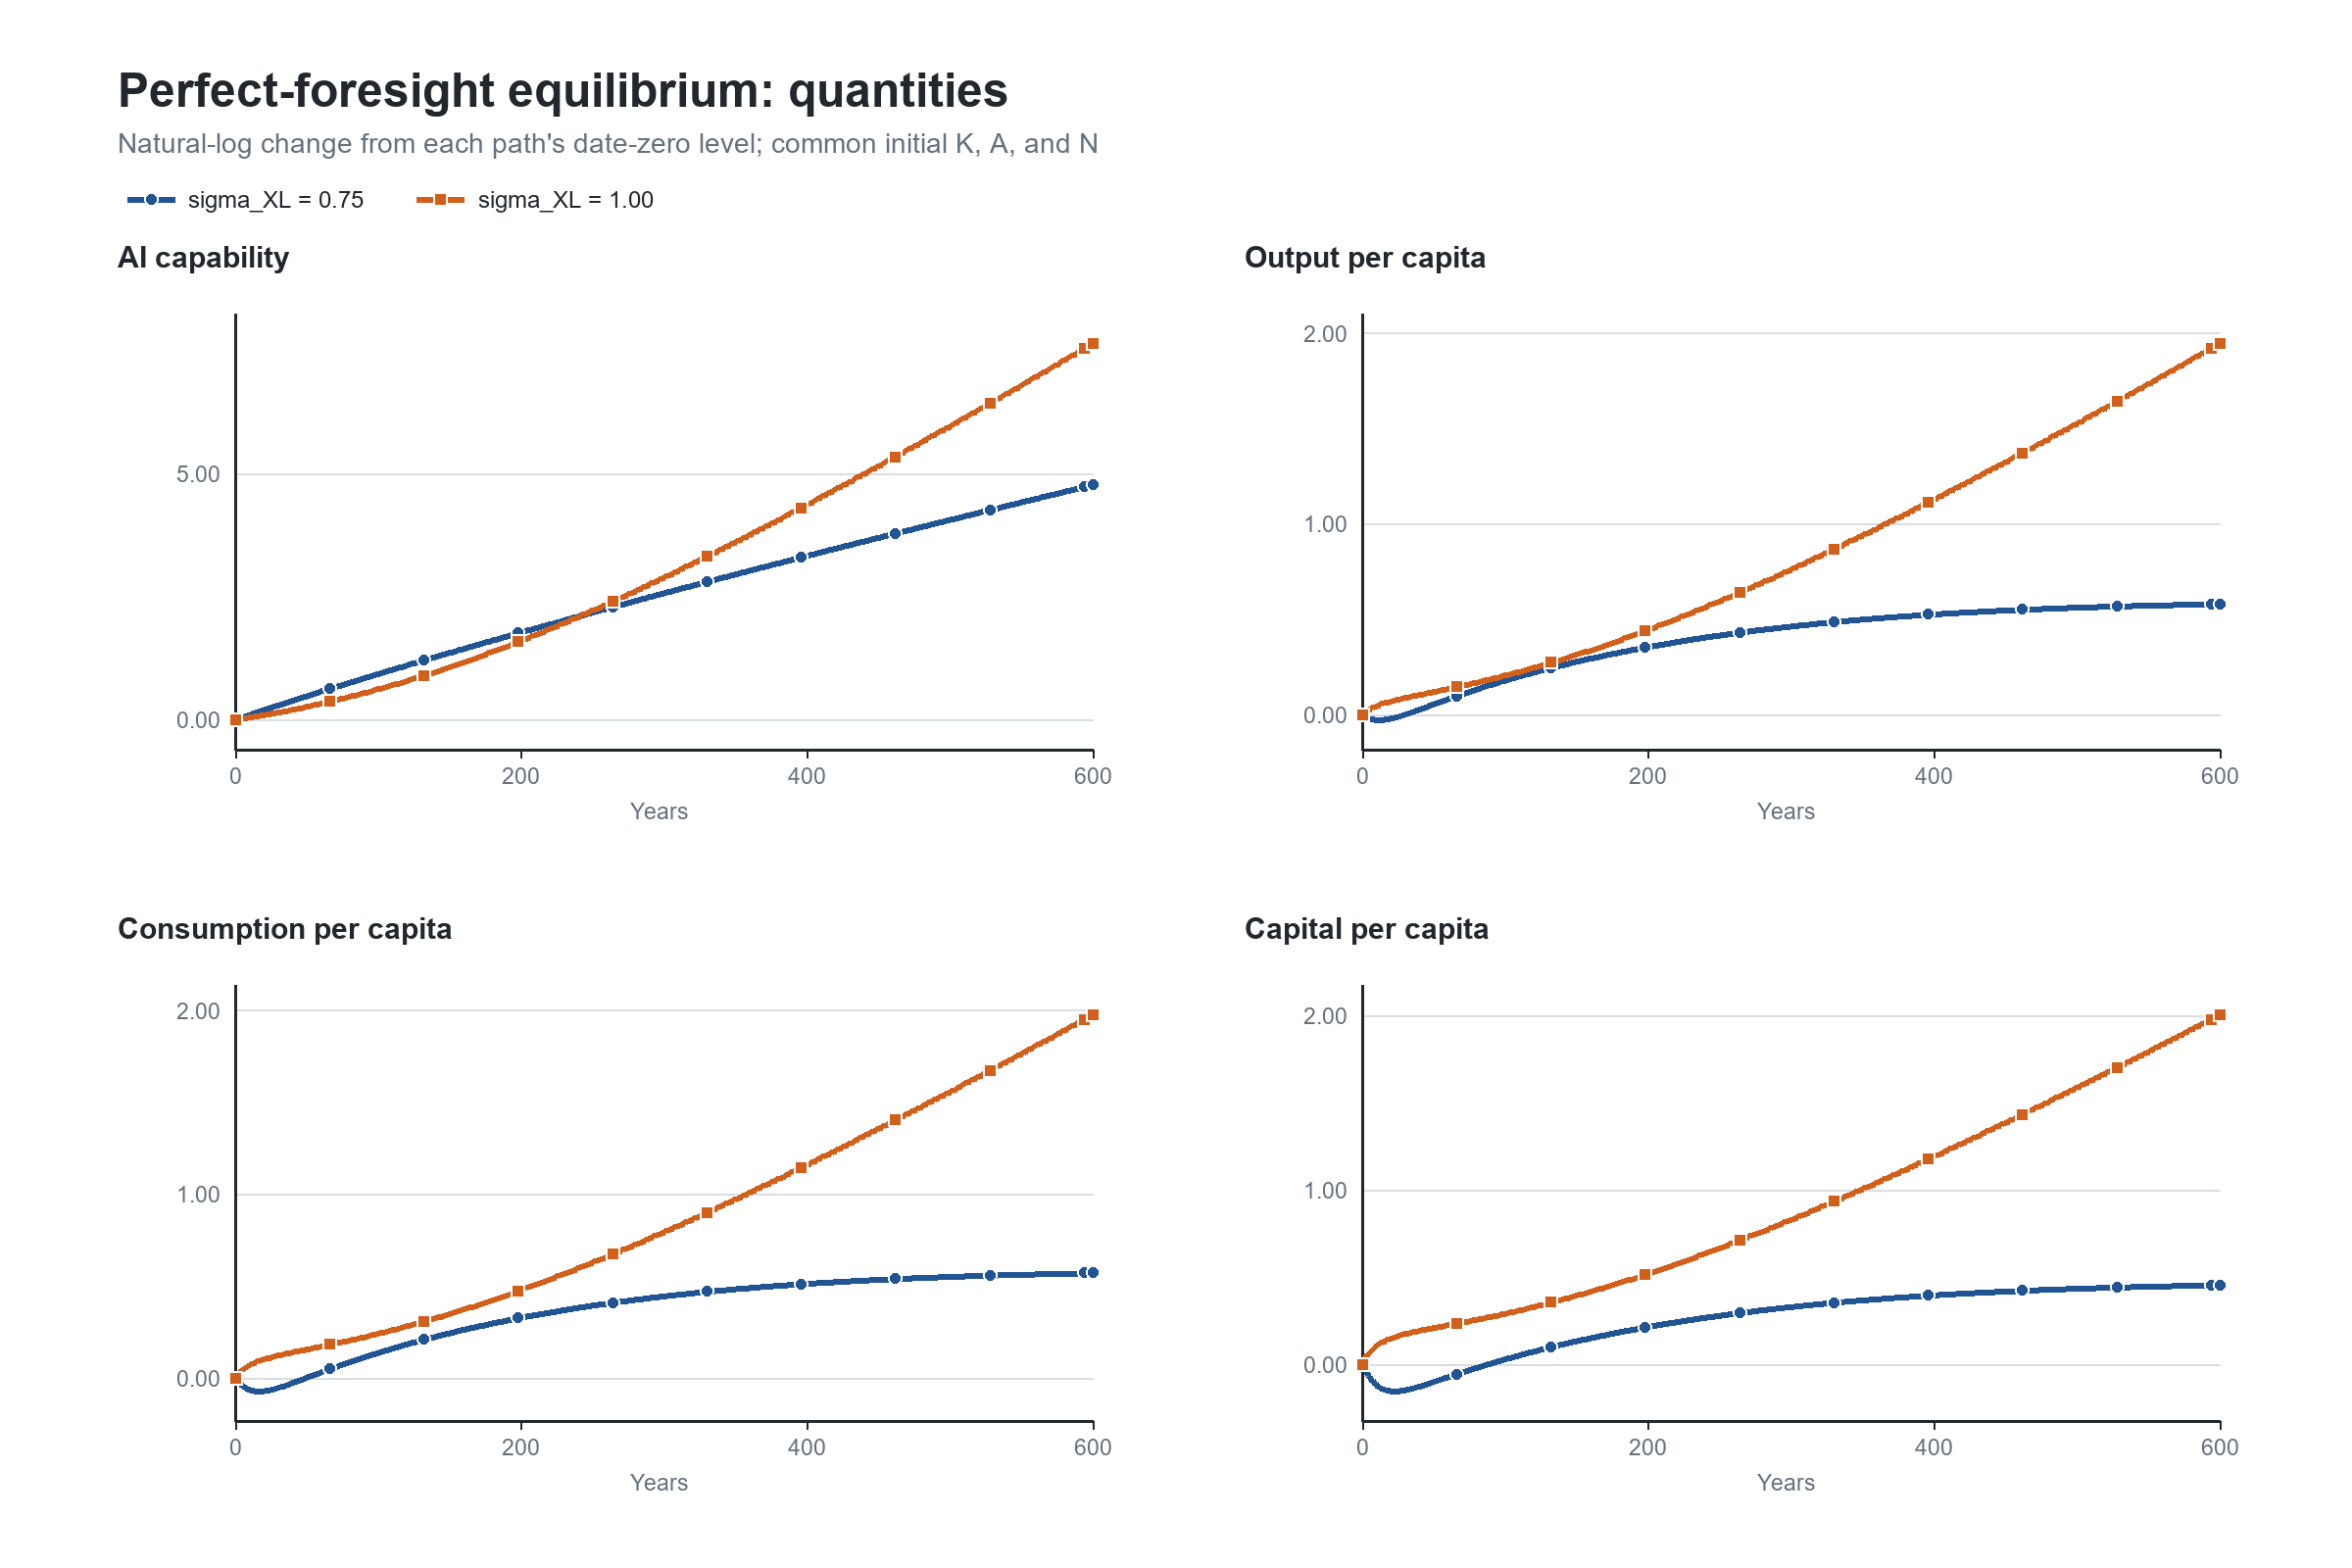
\includegraphics[width=\textwidth]{figures/equilibrium_levels.png}
    \caption{Equilibrium quantities. Each panel reports the natural-log change
    relative to the path's date-zero value. Both paths satisfy the
    household and developer optimality conditions.}
    \label{fig:equilibrium-levels}
\end{figure}

Figure~\ref{fig:equilibrium-growth-rates} makes the complementarity result precise.
When $\sigma_{XL}=0.75$, output-per-capita growth is not zero at every date. It is
negative initially, becomes positive during the recovery, and then converges toward
zero. By year 600 it is 0.0056 percent. Capability growth remains positive and is
close to its analytical limit of 0.675 percent. The experiment therefore
illustrates the production bottleneck characterized in conditional
result~\ref{cond:nonunit-ces-steady-states}; it does not prove convergence or
existence of the required equilibrium limit.

The net return satisfies the Euler equation. Along the complementarity path it
converges to 4 percent, the household discount rate, because consumption per capita
eventually stops growing.

\begin{figure}[H]
    \centering
    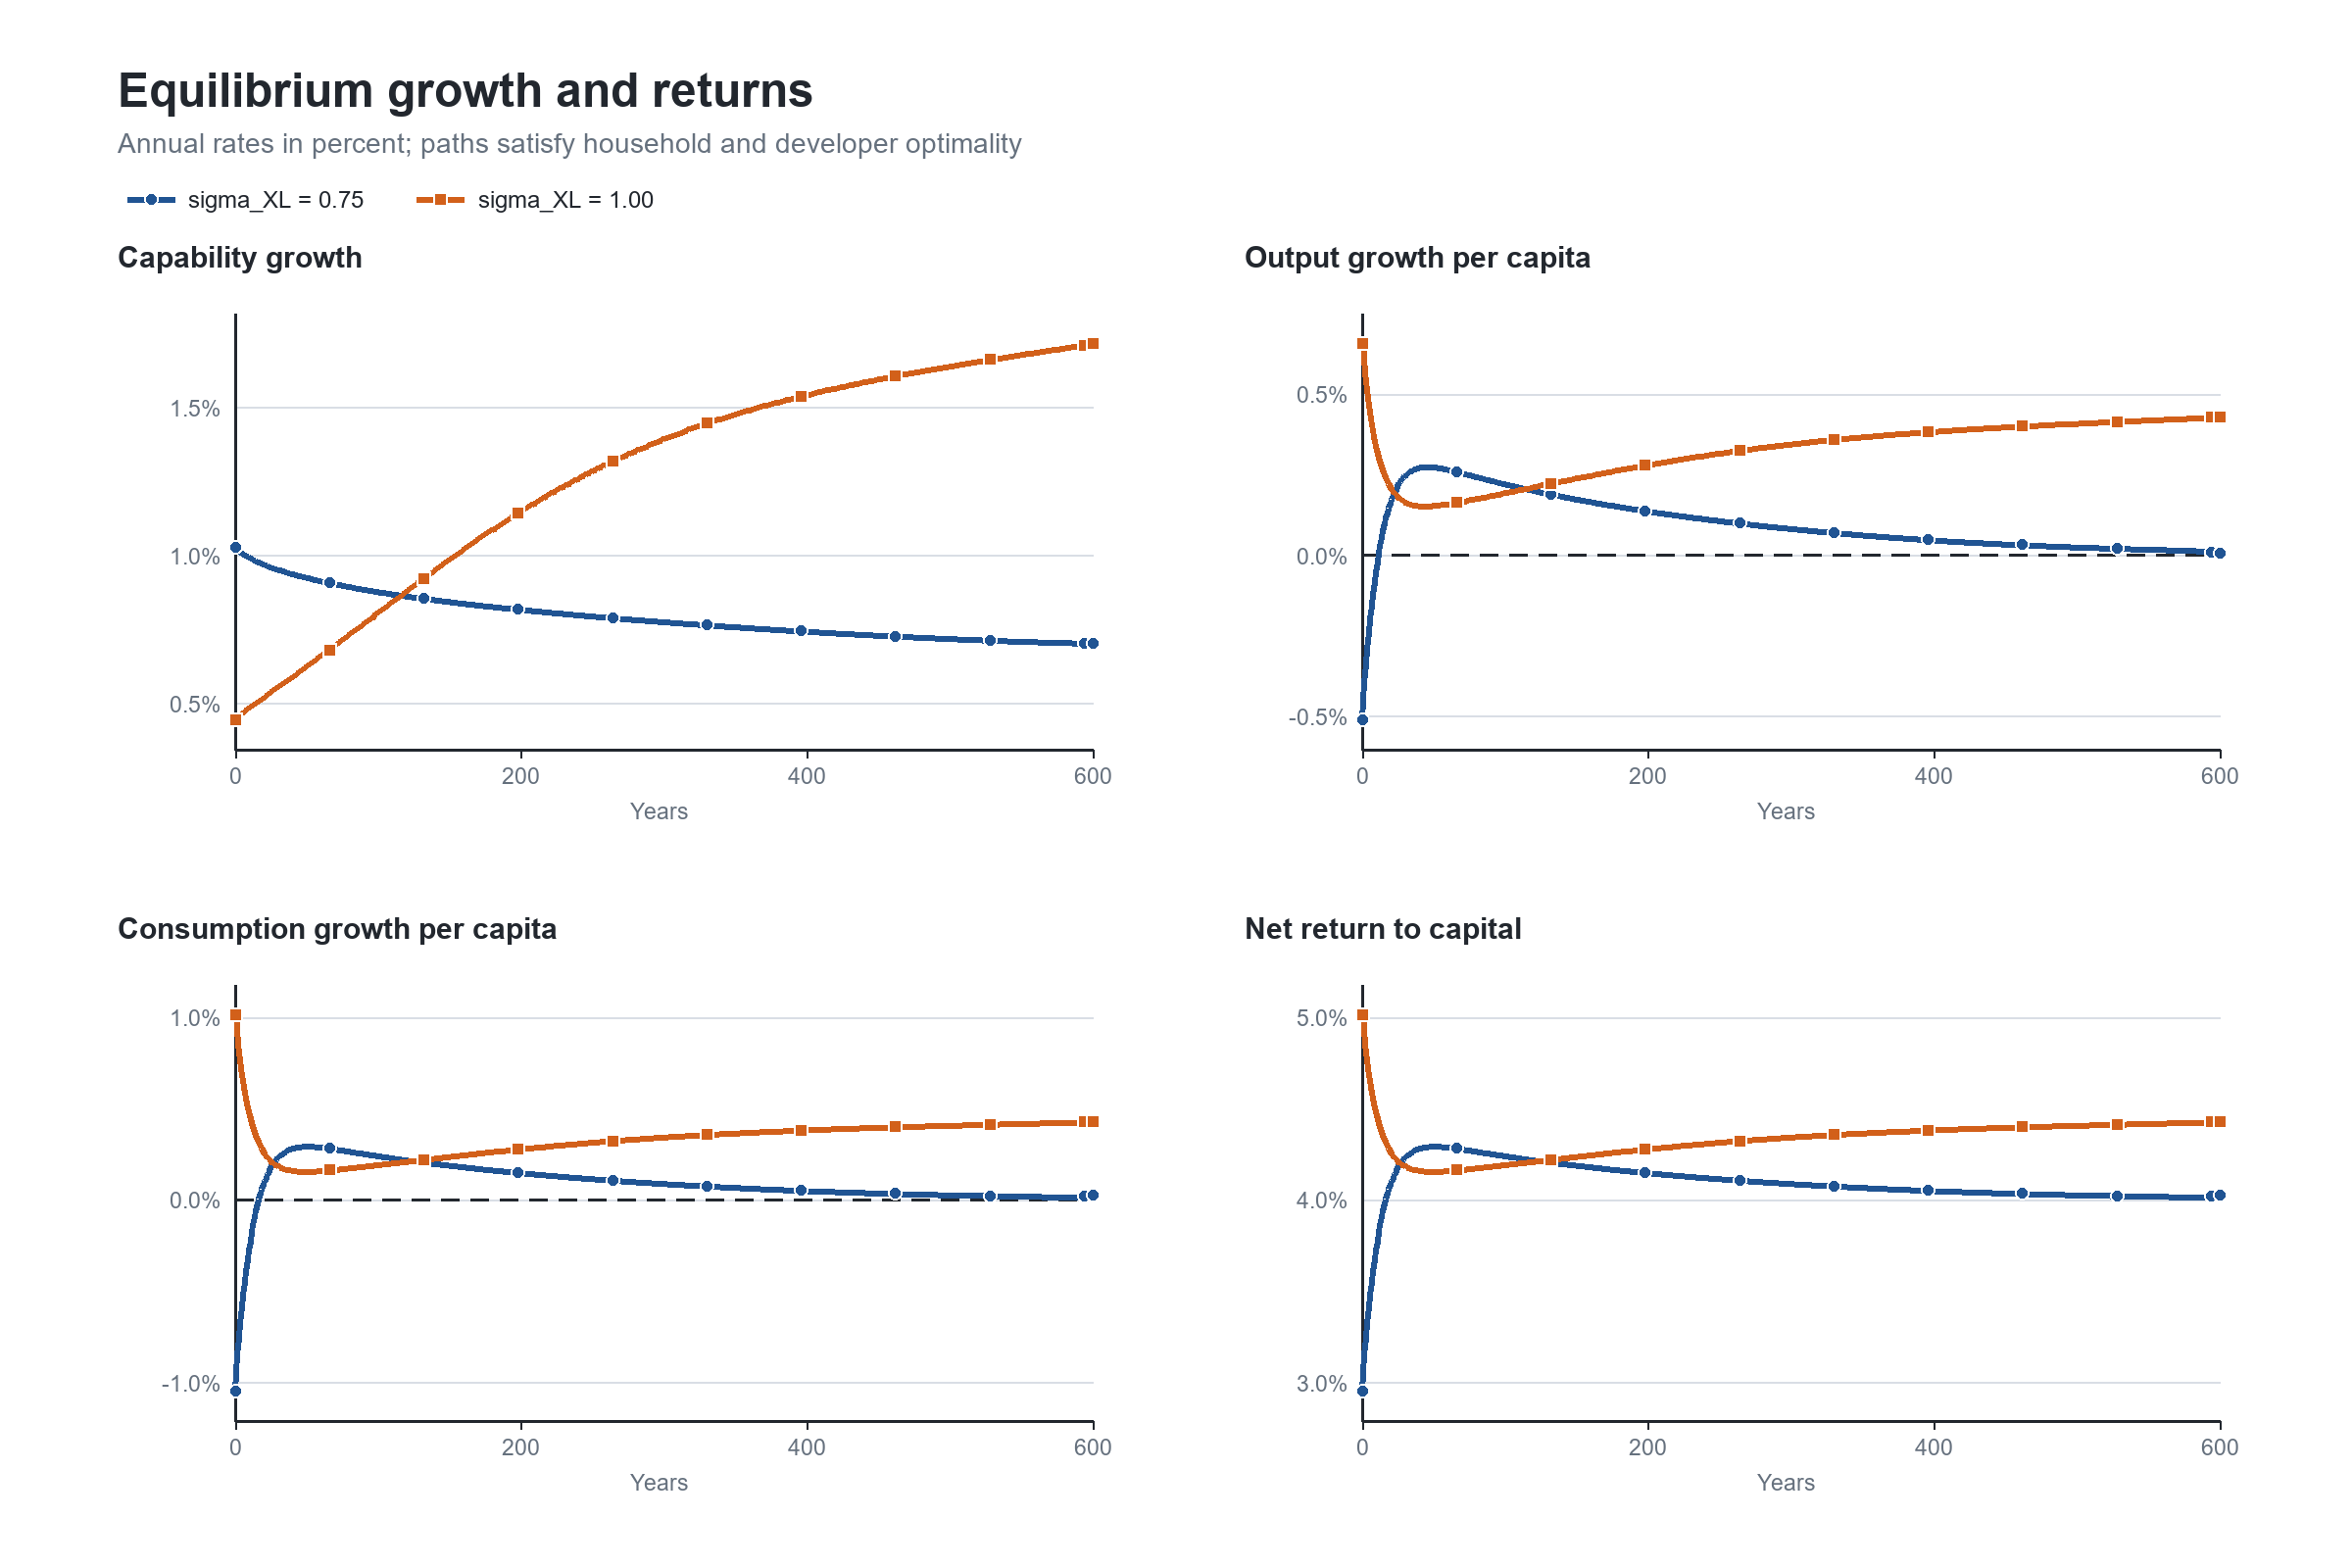
\includegraphics[width=\textwidth]{figures/equilibrium_growth_rates.png}
    \caption{Equilibrium growth rates and the net return to capital. Rates are
    annual. The dashed line marks zero per-capita growth.}
    \label{fig:equilibrium-growth-rates}
\end{figure}

\subsection{Case II: human-essential research at unit production elasticity}
\label{sec:case-human-essential}

\subsubsection{Analytical characterization}

Set $\sigma_{XL}=\sigma_{HM}=1$. The automated contribution to effective research
is then the constant $\omega_M$, so human research remains essential even when
$H/M$ tends to zero. Equations~\eqref{eq:full-cd-ga}--
\eqref{eq:fully-cd-growth-rates} give the candidate constant growth rates. Positive
finite capability growth requires $D_{\mathrm{CD}}>0$, and an interior allocation
also requires the consumption-feasibility condition
\eqref{eq:fully-cd-consumption-feasibility}. On that path, $H/N$ is constant,
$H/M$ declines, and output per capita grows at
$(\omega_X/\omega_L)\eta n/D_{\mathrm{CD}}$. The positivity of
$D_{\mathrm{CD}}$ alone is therefore not an existence theorem.

\subsubsection{Equilibrium transition}

Figure~\ref{fig:equilibrium-research-technology-comparison} holds the production
elasticity and every common parameter fixed and changes only $\sigma_{HM}$. When
$\sigma_{HM}=1$, the automated contribution to effective research remains equal to
$\omega_M=35$ percent. Capability growth converges to 1.738 percent and output and
consumption per capita grow at 0.435 percent. Human research employment converges
to 0.497 percent of the population. The ratio $H/M$ nevertheless converges to zero:
human input becomes small relative to automated input without ceasing to be
essential for effective research. The $\sigma_{HM}=2$ path in the same figure is
analyzed in Case III.

\begin{figure}[H]
    \centering
    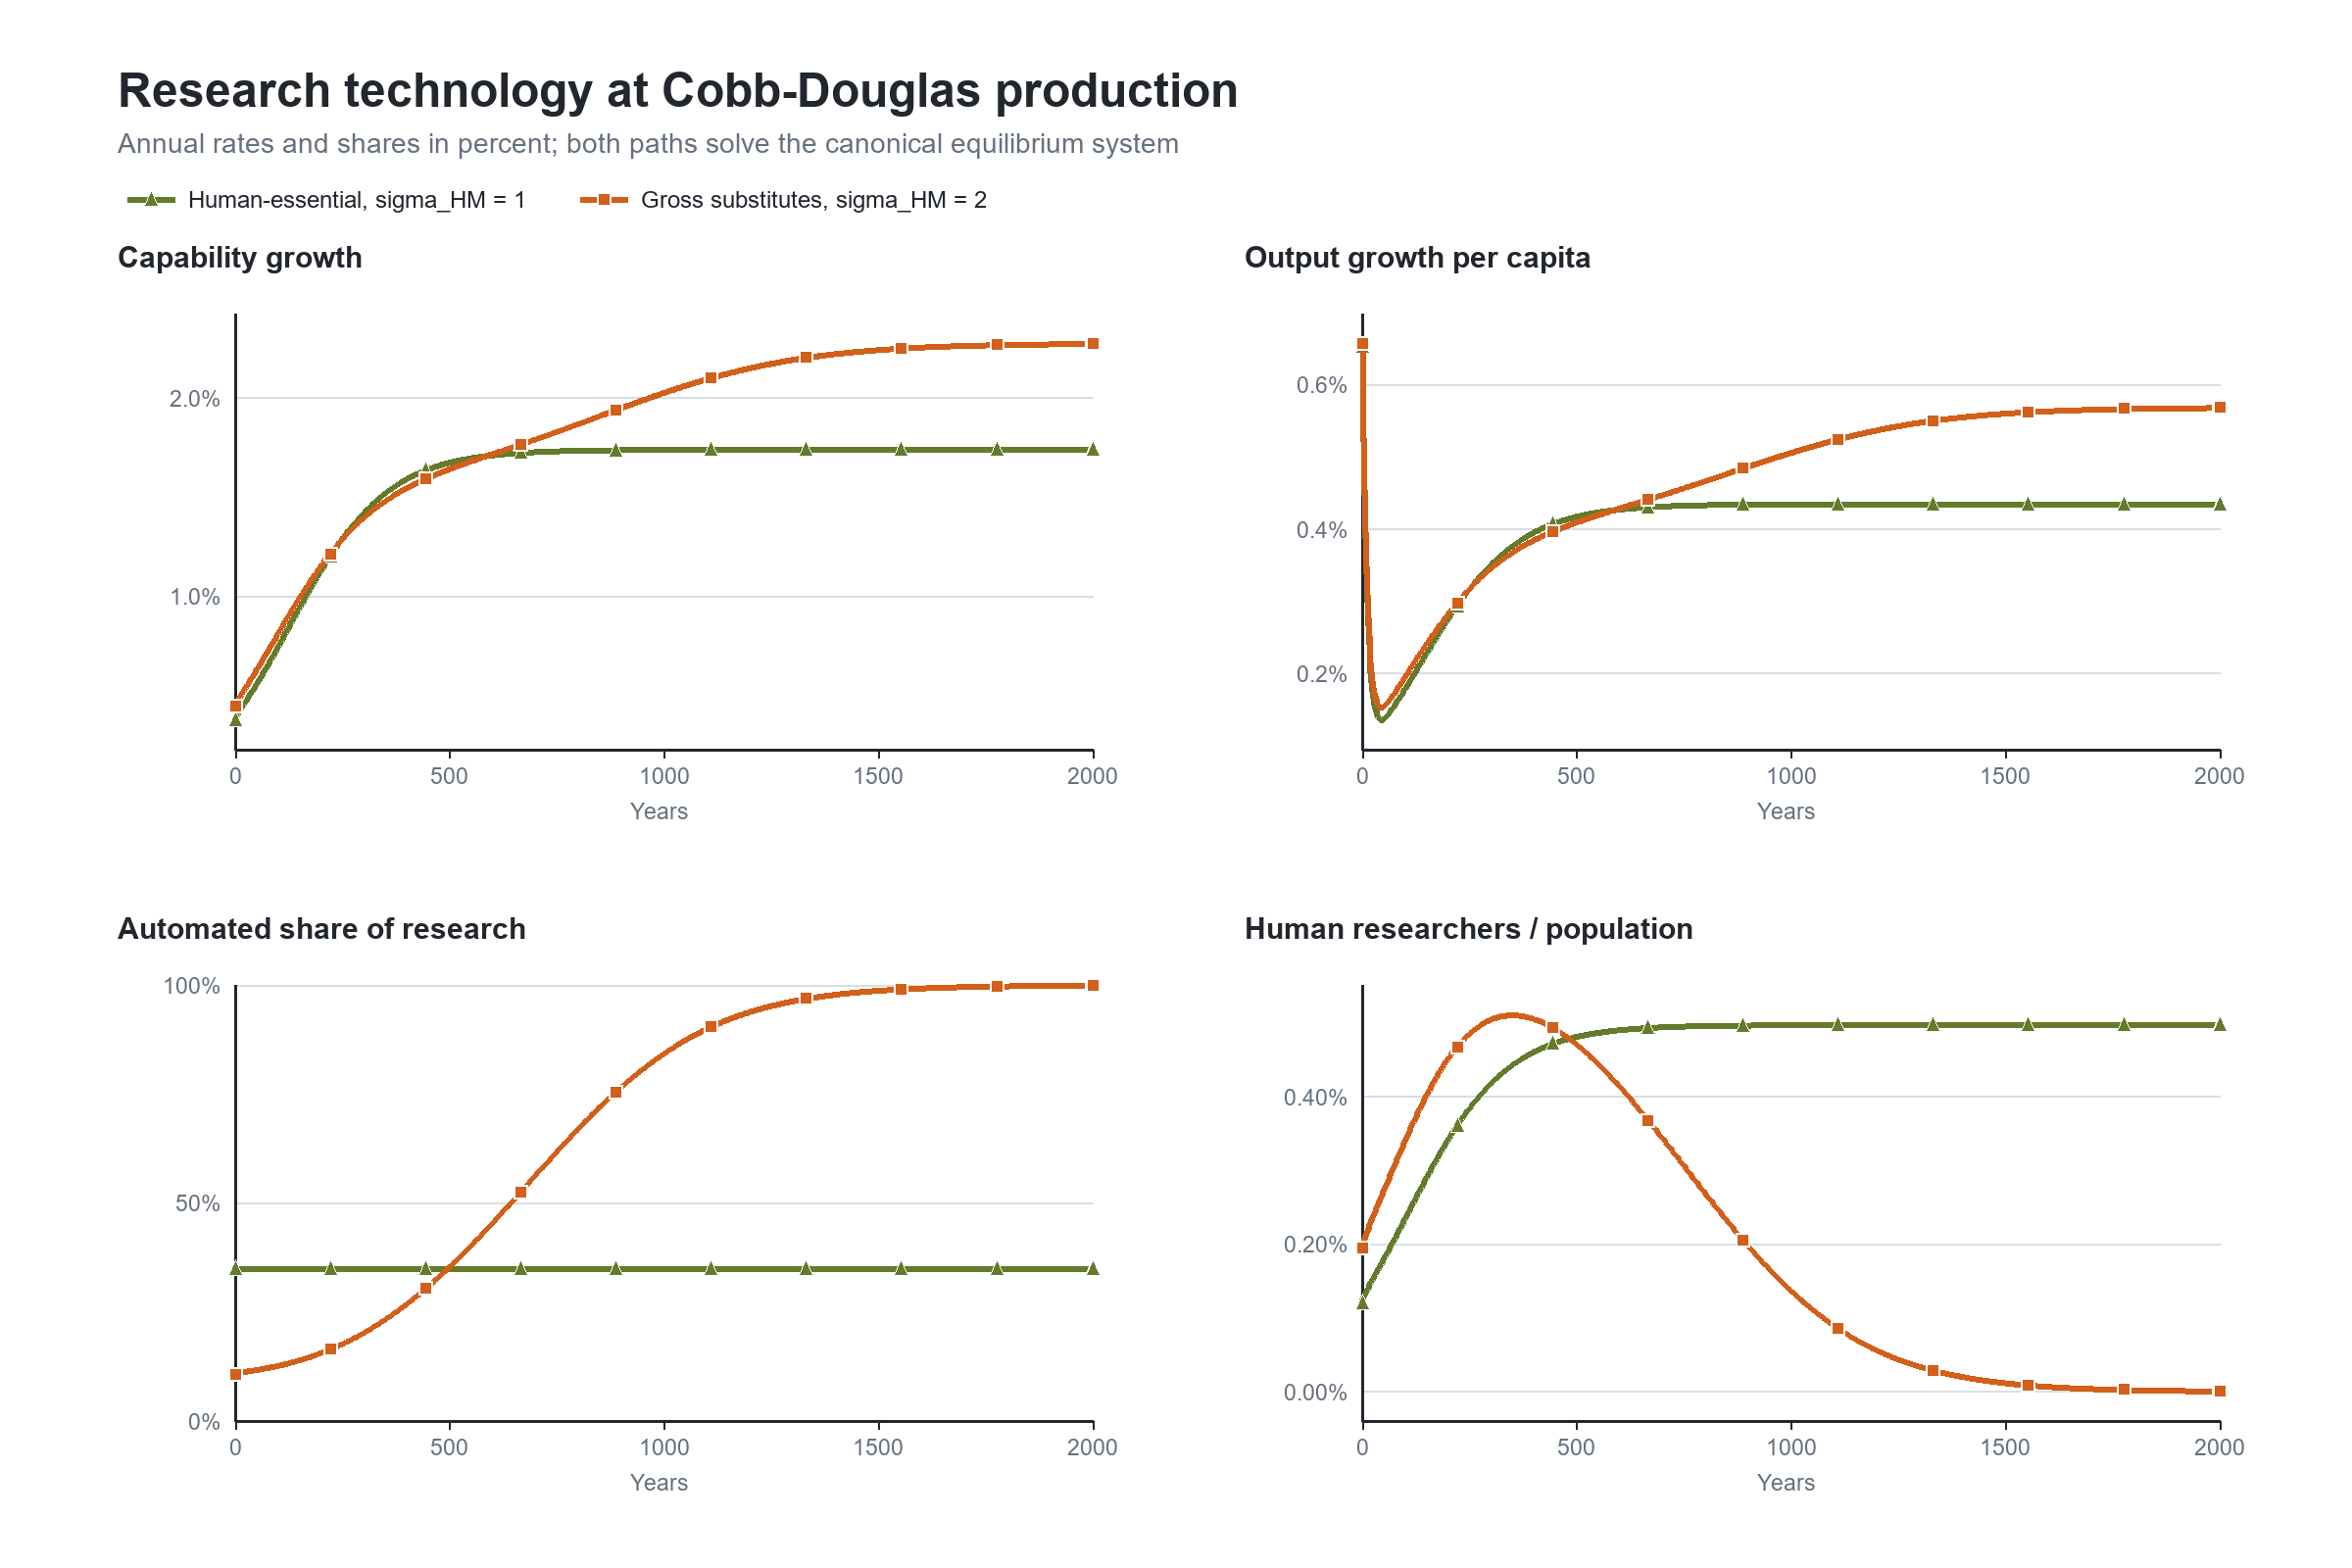
\includegraphics[width=\textwidth]{figures/equilibrium_research_technology_comparison.png}
    \caption{Research technology at Cobb--Douglas production. Both 2,000-year
    paths solve the canonical equilibrium system and share all parameters and
    initial stocks except $\sigma_{HM}$.}
    \label{fig:equilibrium-research-technology-comparison}
\end{figure}

\subsection{Case III: substitutable research at unit production elasticity}
\label{sec:case-substitutable-research}

\subsubsection{Analytical characterization}

Now set $\sigma_{XL}=1$ and $\sigma_{HM}>1$. Conditional
result~\ref{cond:ai-dominated-cd-limit} characterizes any nondegenerate
constant-growth limit in which the automated contribution tends to one. Such a
limit requires $D_{\mathrm{AI}}>0$. Capability growth and output-per-capita growth
are then $\eta n/D_{\mathrm{AI}}$ and
$(\omega_X/\omega_L)\eta n/D_{\mathrm{AI}}$, respectively. Unlike Case II, the
research contribution $s^M_t$ is endogenous and the feedback denominator moves
from its human-dominated value toward $D_{\mathrm{AI}}$. These statements are
conditional on the stated limit; the equilibrium computation determines whether
the transition actually approaches it from the chosen initial stocks.

\subsubsection{Equilibrium transition}

Along the equilibrium path, capability growth rises from 0.445 percent to 1.716
percent during the first 600 years and reaches 2.271 percent by year 2,000. Output-
and consumption-per-capita growth approach the analytical value of 0.568 percent,
and the net return converges to 4.568 percent. In
Figure~\ref{fig:equilibrium-research-technology-comparison}, the automated
contribution rises toward one and human research employment converges to zero.
Capability growth converges to 2.274 percent rather than the human-essential limit
of 1.738 percent. Gross substitution in research therefore changes both who
performs research and the strength of the feedback from output to capability.

\subsection{Cross-case comparisons: production, labor, and monopoly}

The next figures compare Cases I and III over a common 600-year window. They are
reported separately because the production chain, factor shares, resource
allocation, and monopoly outcomes are meaningful precisely as comparisons across
production regimes. Case II was isolated above to compare research technologies,
and Case IV is analyzed below on its endogenous free-boundary horizon.

Figure~\ref{fig:equilibrium-production-chain} follows the production tree rather
than placing all growing quantities in one panel. Under complementarity,
inference compute per capita falls even though capability rises. AI services per
capita still increase because each unit of compute becomes more productive, but
the service composite approaches a finite level. Under Cobb--Douglas production,
inference compute, AI services, and the service composite eventually become
log-linear. In both cases the real price of AI services falls, but much faster in
the Cobb--Douglas path.

\begin{figure}[H]
    \centering
    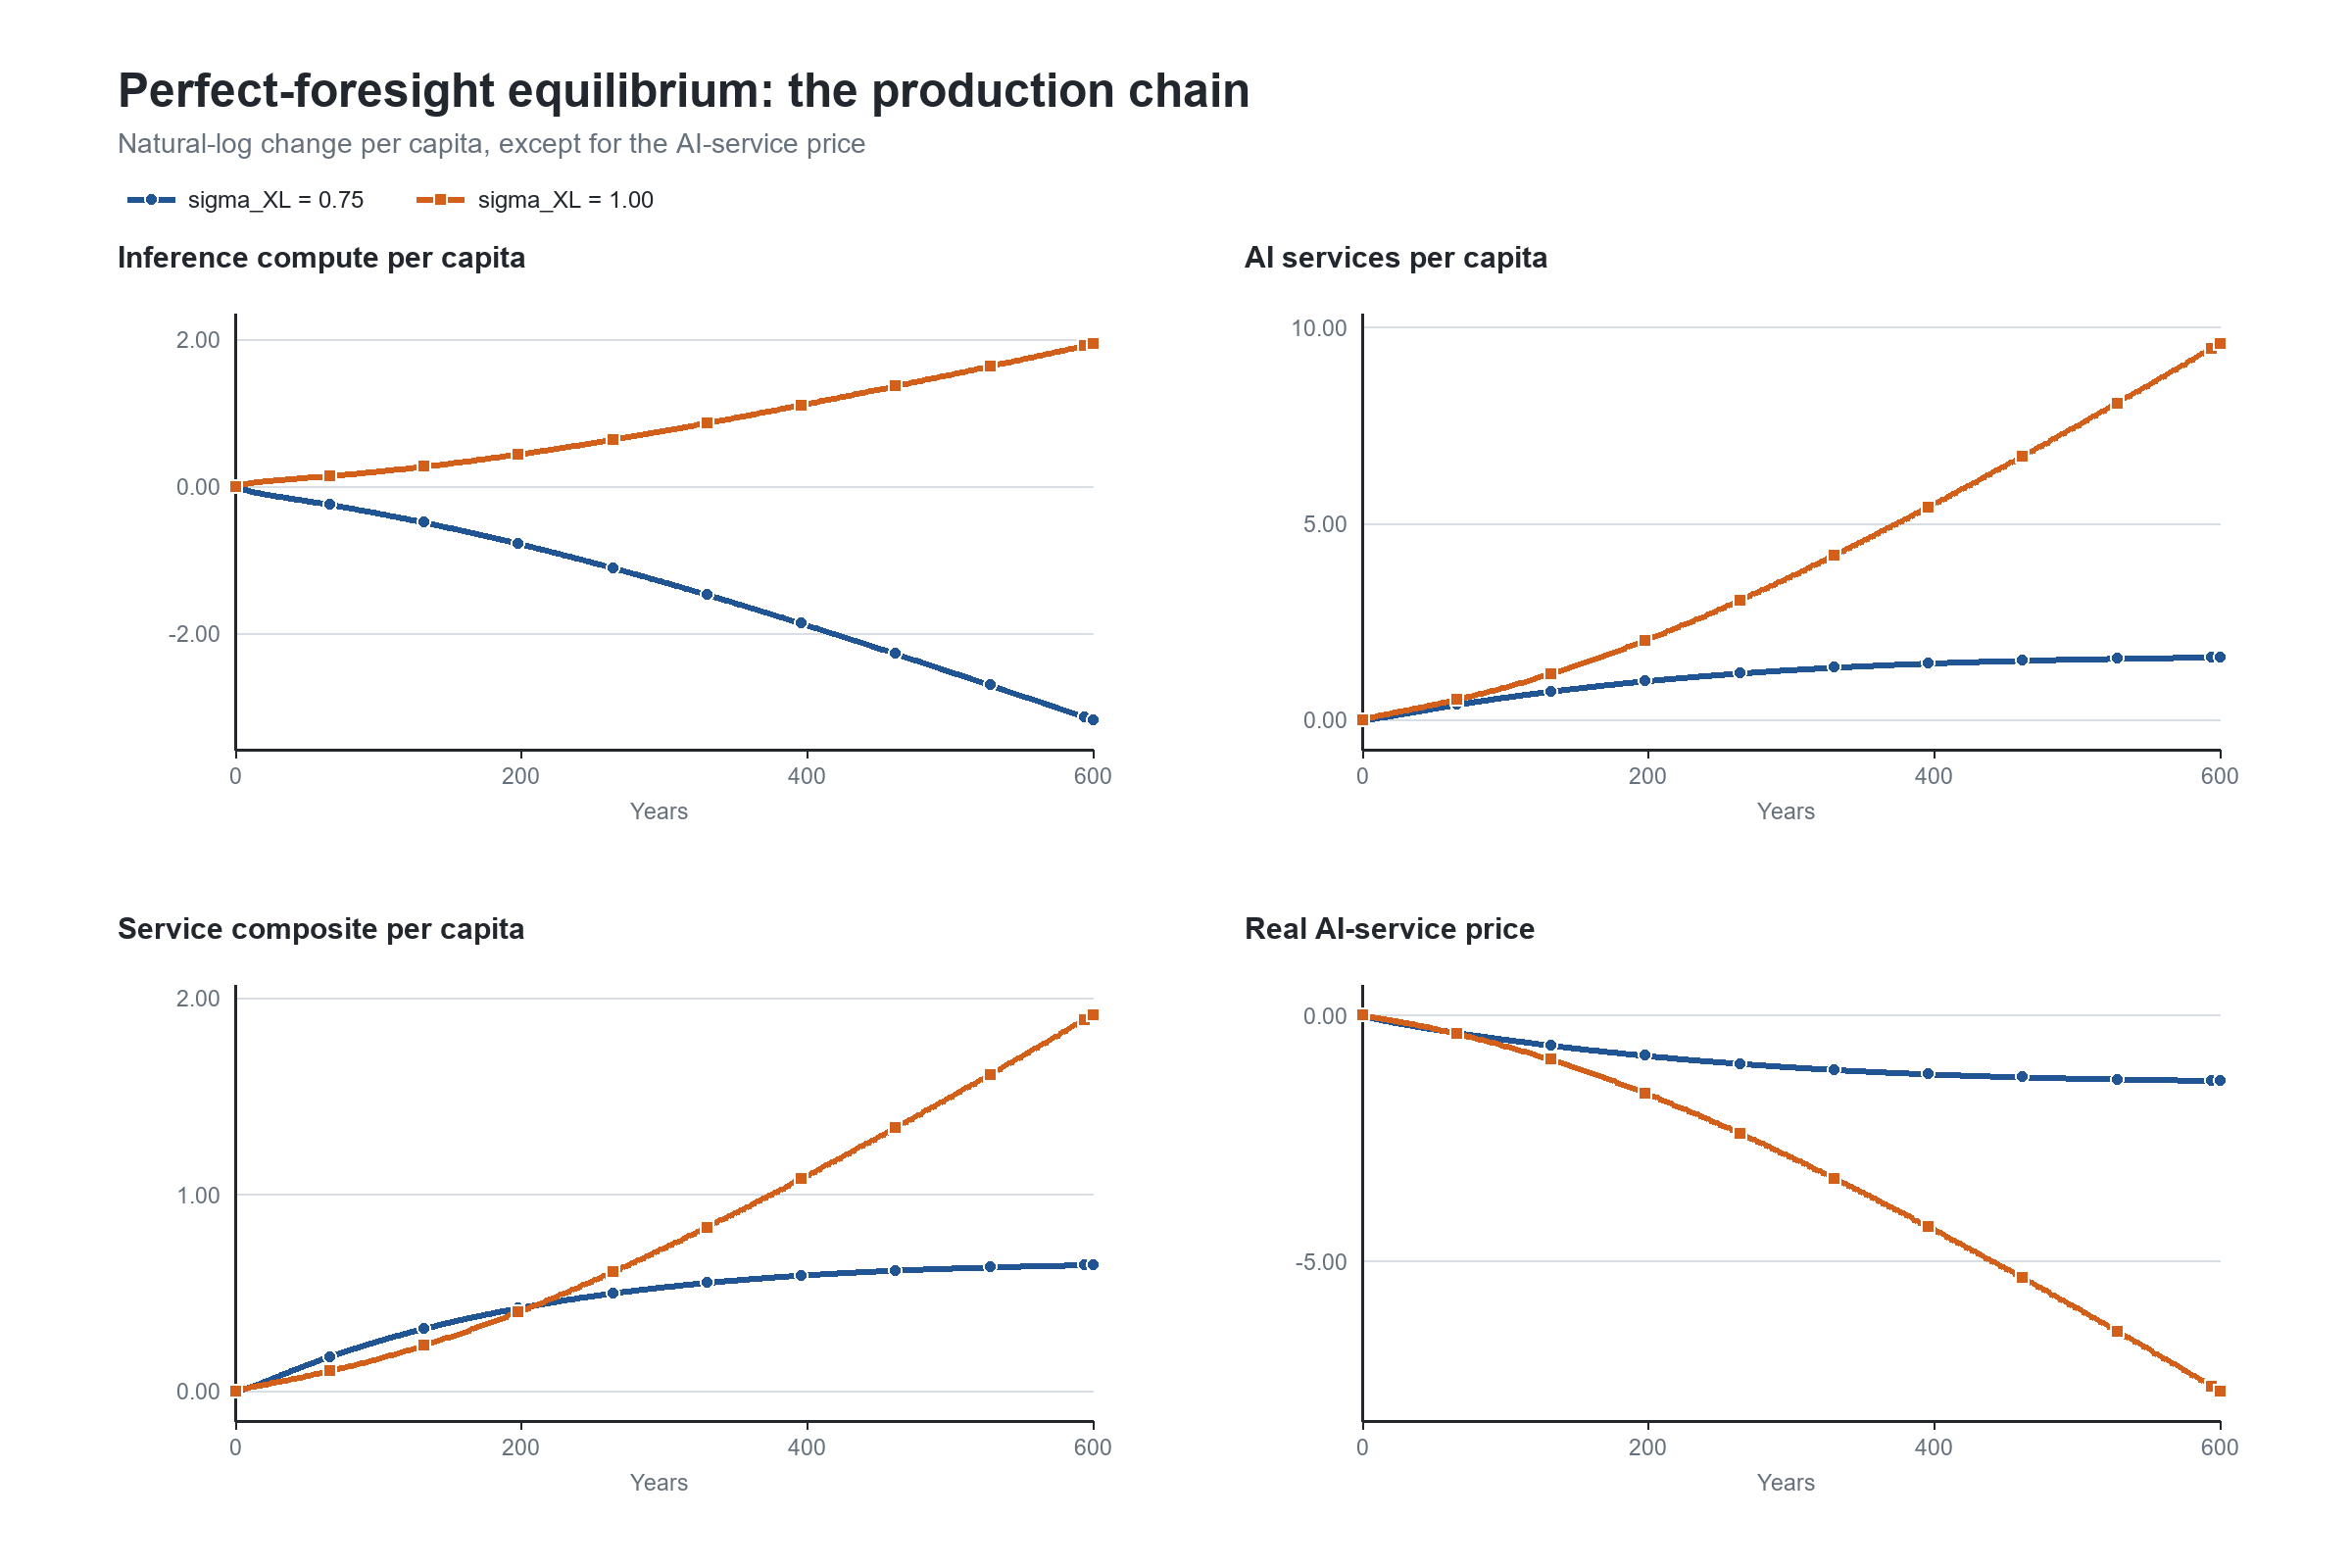
\includegraphics[width=\textwidth]{figures/equilibrium_production_chain.png}
    \caption{The equilibrium production chain. Quantity panels report
    natural-log changes per capita; the last panel reports the natural-log change
    in the real price of AI services.}
    \label{fig:equilibrium-production-chain}
\end{figure}

Figure~\ref{fig:equilibrium-factor-shares} reports the allocation of labor and
research. With $\sigma_{XL}=0.75$, the production-labor share rises from 36.05 to
44.46 percent as labor becomes the production bottleneck. The aggregate labor share
rises by almost the same amount because human research employment falls from 1.38
percent to 0.016 percent of the population. The automated contribution to research
increases only from 6.02 to 12.23 percent. A research elasticity above one does not
make automation dominant when the wage remains bounded.

Under Cobb--Douglas production, the production-labor share remains fixed at 53.60
percent. The automated research share rises from 10.60 percent to 45.35 percent by
year 600 and to 99.93 percent by year 2,000. Human research employment is
non-monotone: it rises from 0.19 percent of the population to approximately 0.5
percent and then tends to zero. The development industry can therefore expand its
use of human researchers during part of the automation transition even though
human input eventually becomes negligible relative to automated research.

\begin{figure}[H]
    \centering
    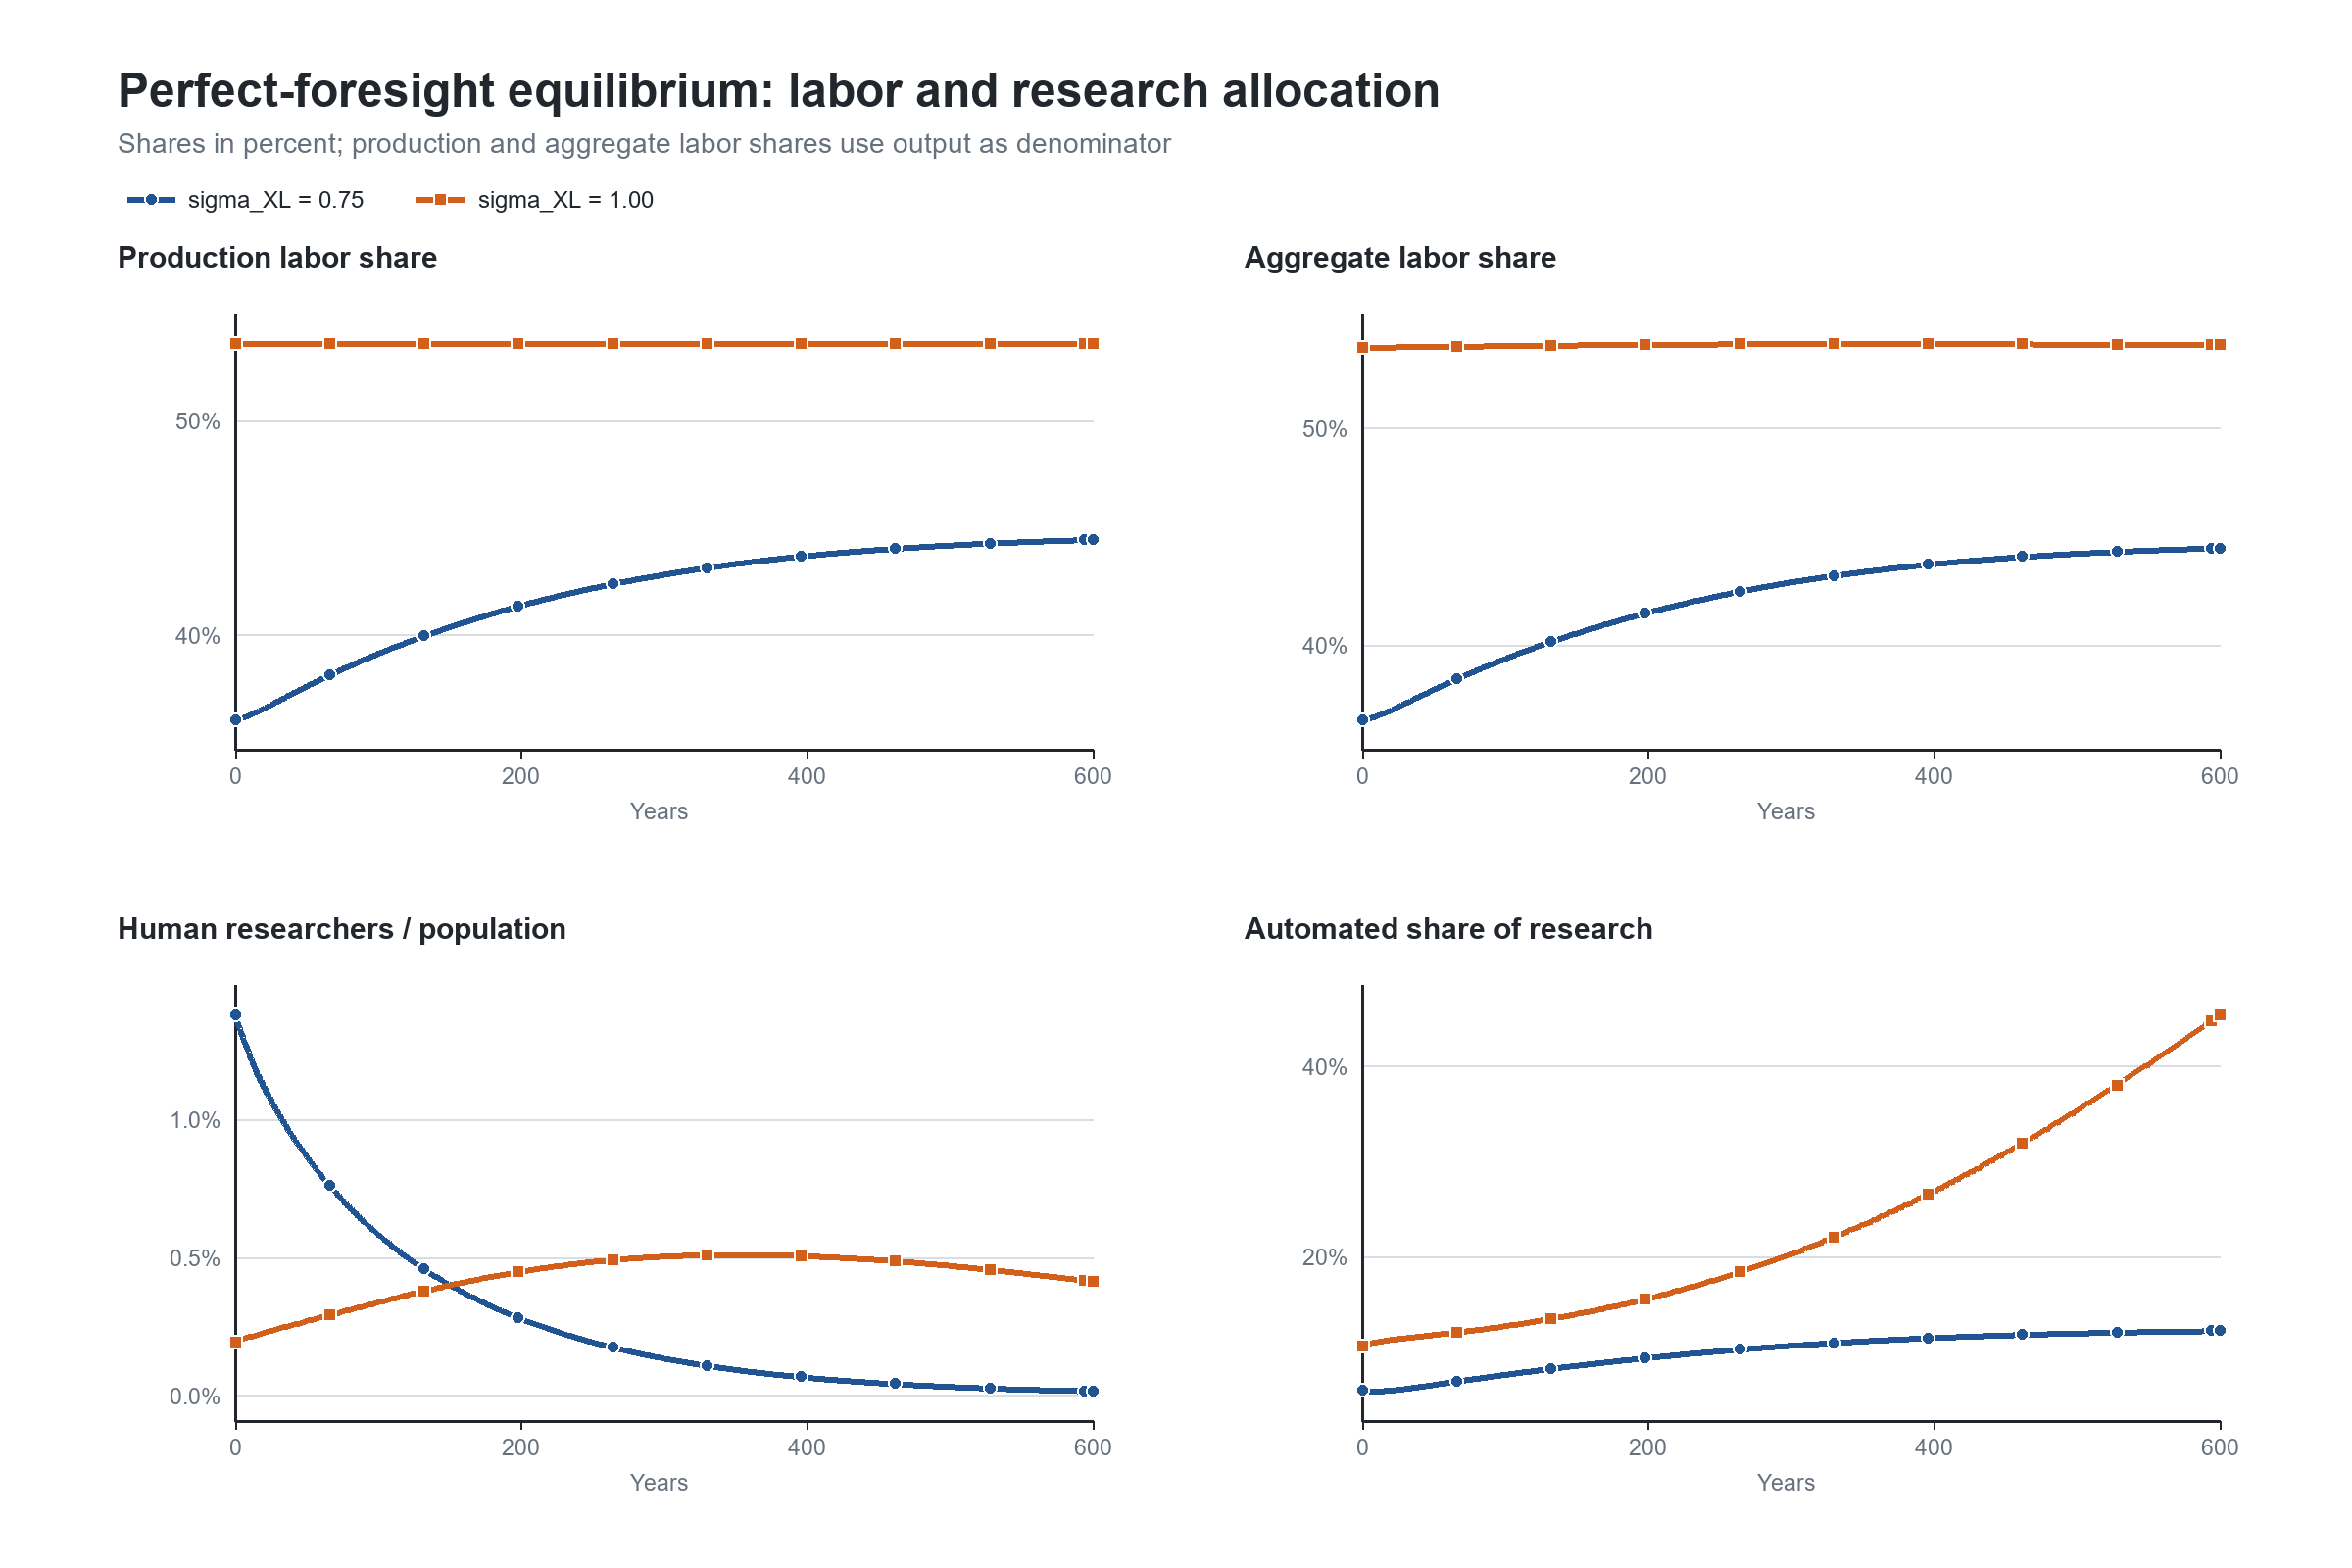
\includegraphics[width=\textwidth]{figures/equilibrium_factor_shares.png}
    \caption{Labor-income shares and the equilibrium research allocation. The
    aggregate labor share includes both production workers and human researchers.}
    \label{fig:equilibrium-factor-shares}
\end{figure}

Figure~\ref{fig:equilibrium-research-chain} makes the distinction between scale
and composition explicit. Under complementarity, human, automated, and effective
research all contract per capita, even though the automated contribution to the
research CES rises. Under Cobb--Douglas production, human research per capita is
temporarily hump-shaped while automated and effective research expand. The
human-to-machine ratio falls in both paths, but the aggregate scale consequences
are opposite. A falling $H/M$ is therefore not, by itself, evidence that the AI
development sector is expanding.

\begin{figure}[H]
    \centering
    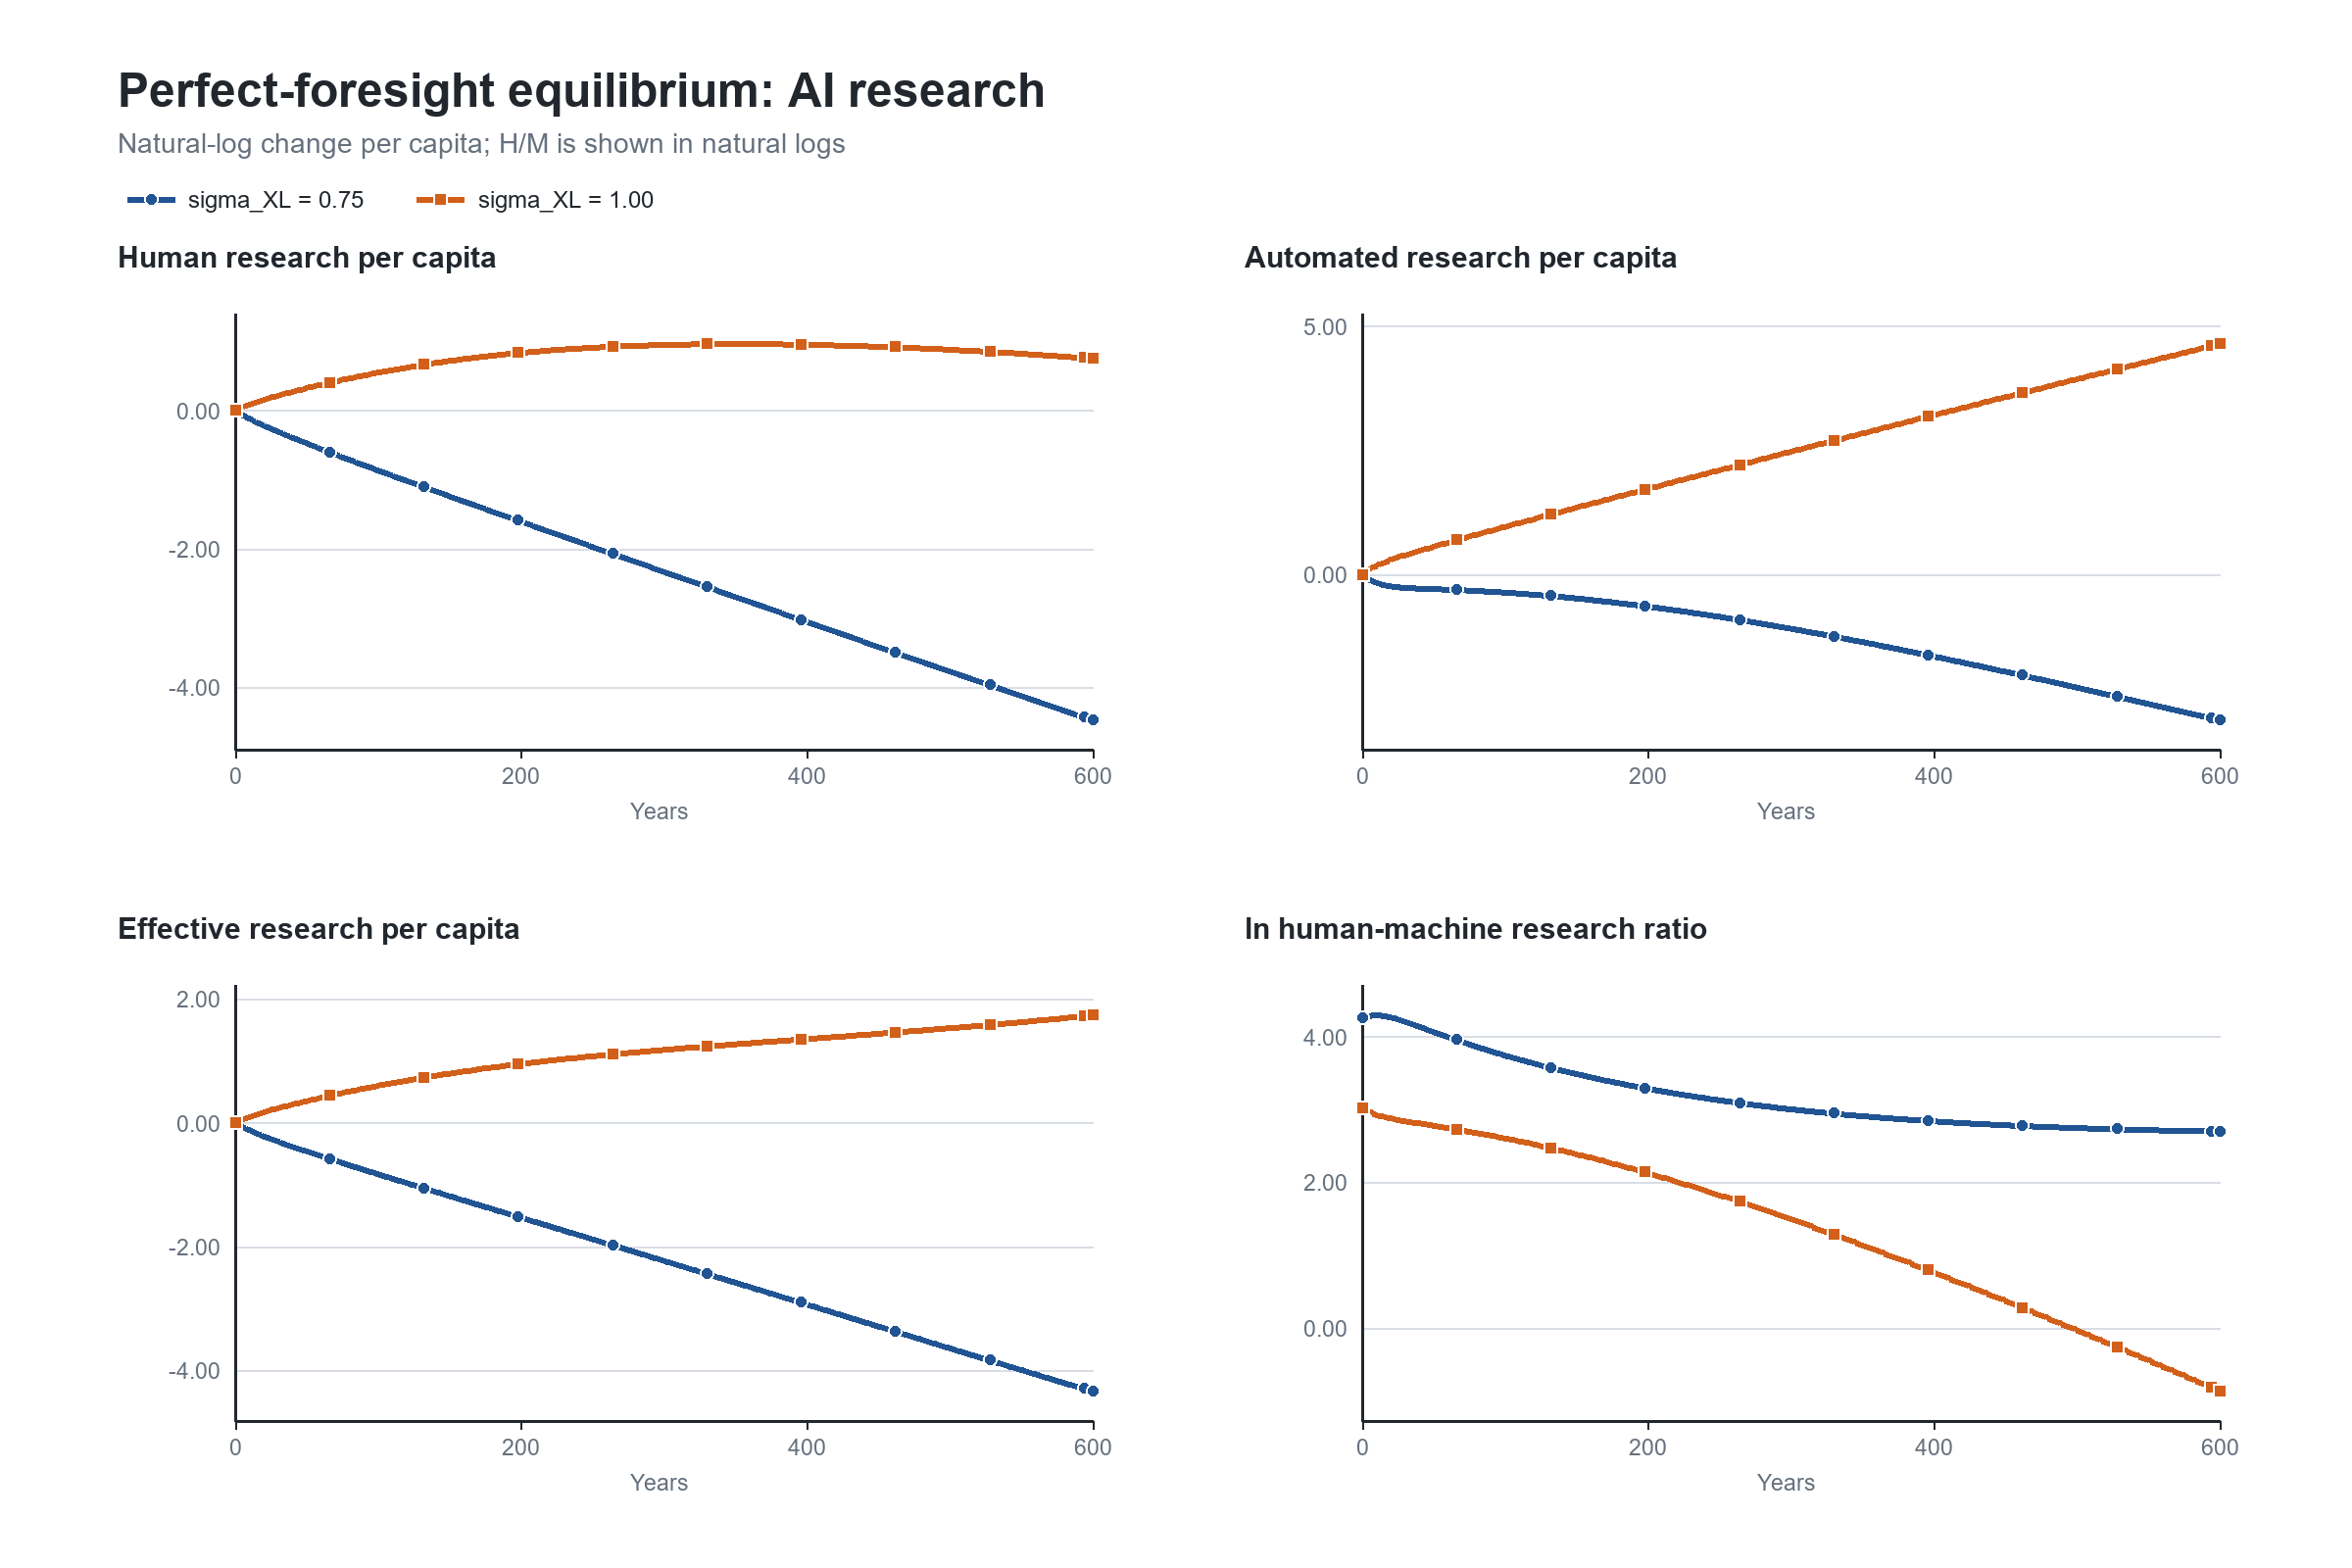
\includegraphics[width=\textwidth]{figures/equilibrium_research_chain.png}
    \caption{The equilibrium research chain. The first three panels report
    natural-log changes per capita; the final panel reports $\ln(H/M)$.}
    \label{fig:equilibrium-research-chain}
\end{figure}

The 600-year comparison understates how slowly the Cobb--Douglas limit emerges.
Figure~\ref{fig:equilibrium-cd-long-run} therefore reports the full 2,000-year
path separately. Capability and output growth approach constants only after the
automated contribution to research has moved close to one and human research has
become negligible relative to population. This separate long-horizon panel avoids
compressing the economically relevant first centuries of the complementarity
experiment.

\begin{figure}[H]
    \centering
    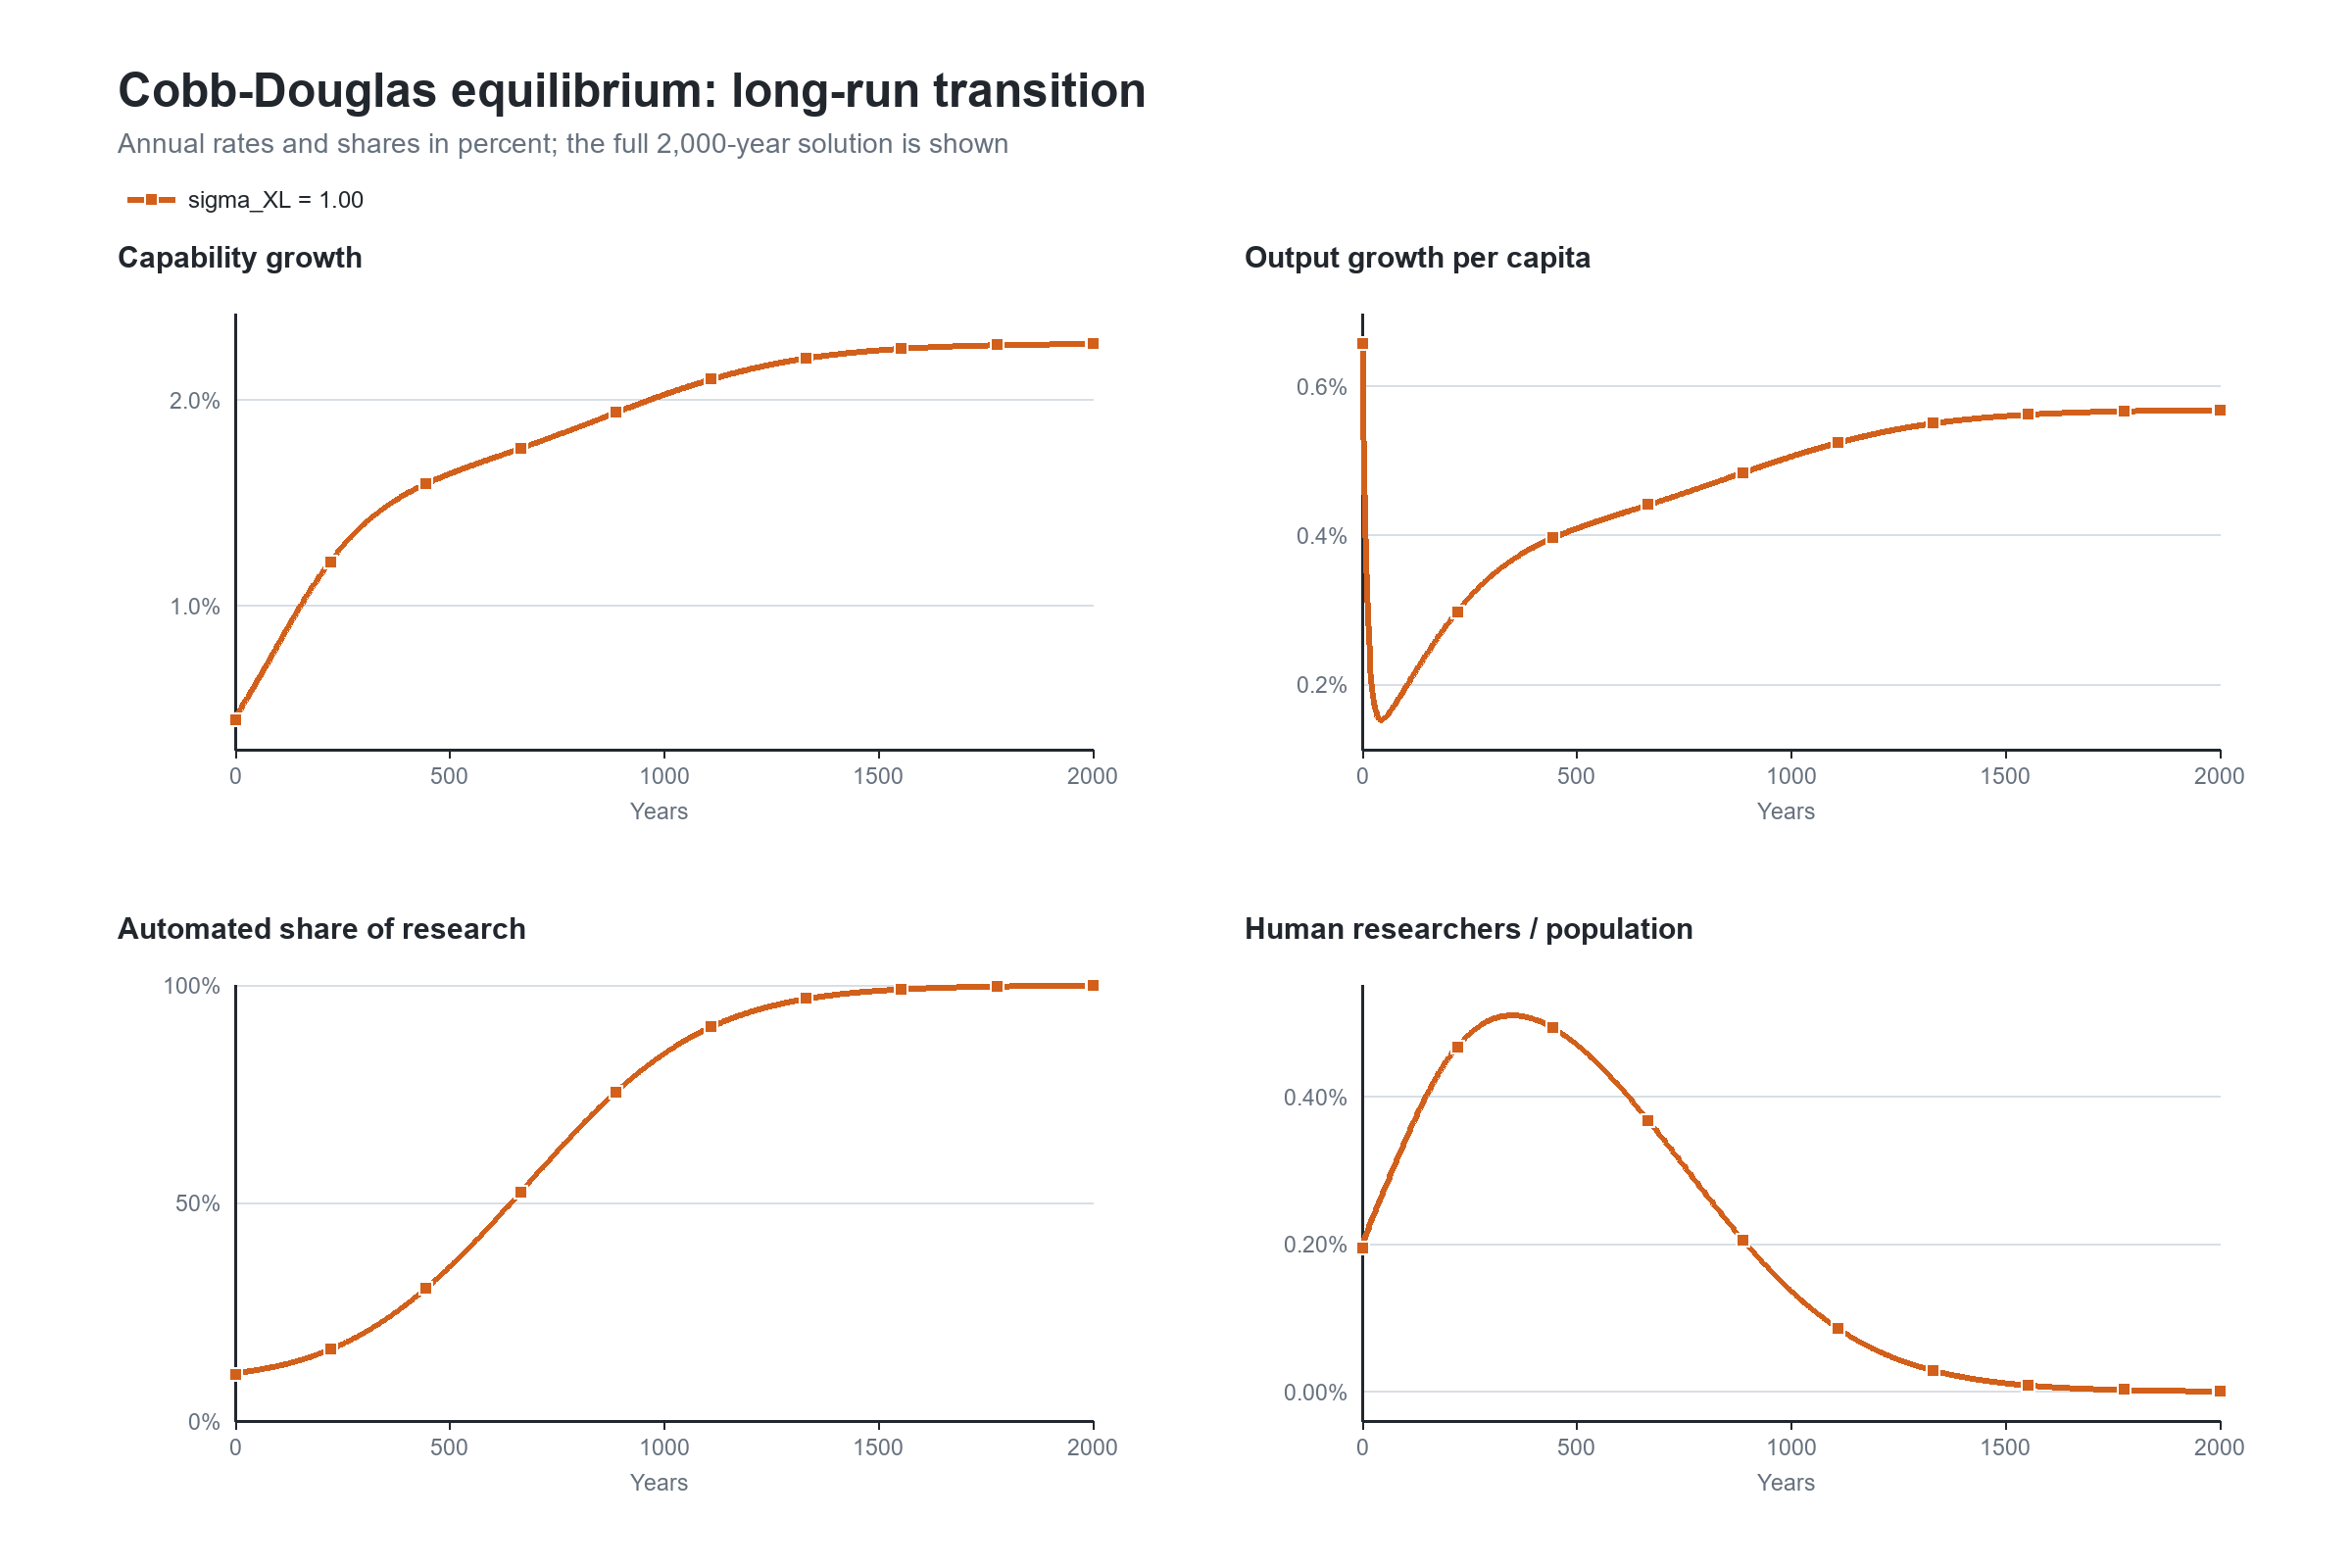
\includegraphics[width=\textwidth]{figures/equilibrium_cobb_douglas_long_run.png}
    \caption{Long-run Cobb--Douglas transition. The figure shows the complete
    2,000-year equilibrium solution rather than truncating it to the common
    600-year comparison window.}
    \label{fig:equilibrium-cd-long-run}
\end{figure}

Figures~\ref{fig:equilibrium-resource-allocation} and
\ref{fig:equilibrium-monopoly-block} close the accounting and monopoly blocks.
The four resource shares add to one at every date. Under complementarity,
inference and automated-research spending become negligible relative to output;
under Cobb--Douglas production, inference spending remains constant as a share of
output while automated-research spending gradually rises. Market power also has
different manifestations. With Cobb--Douglas demand the markup and operating
profit share are constant. Under complementarity, the price falls much more slowly
than marginal cost, so the markup rises sharply even as operating profits decline
as a share of output. The markup alone is therefore not a sufficient measure of
the developer's aggregate rents.

\begin{figure}[H]
    \centering
    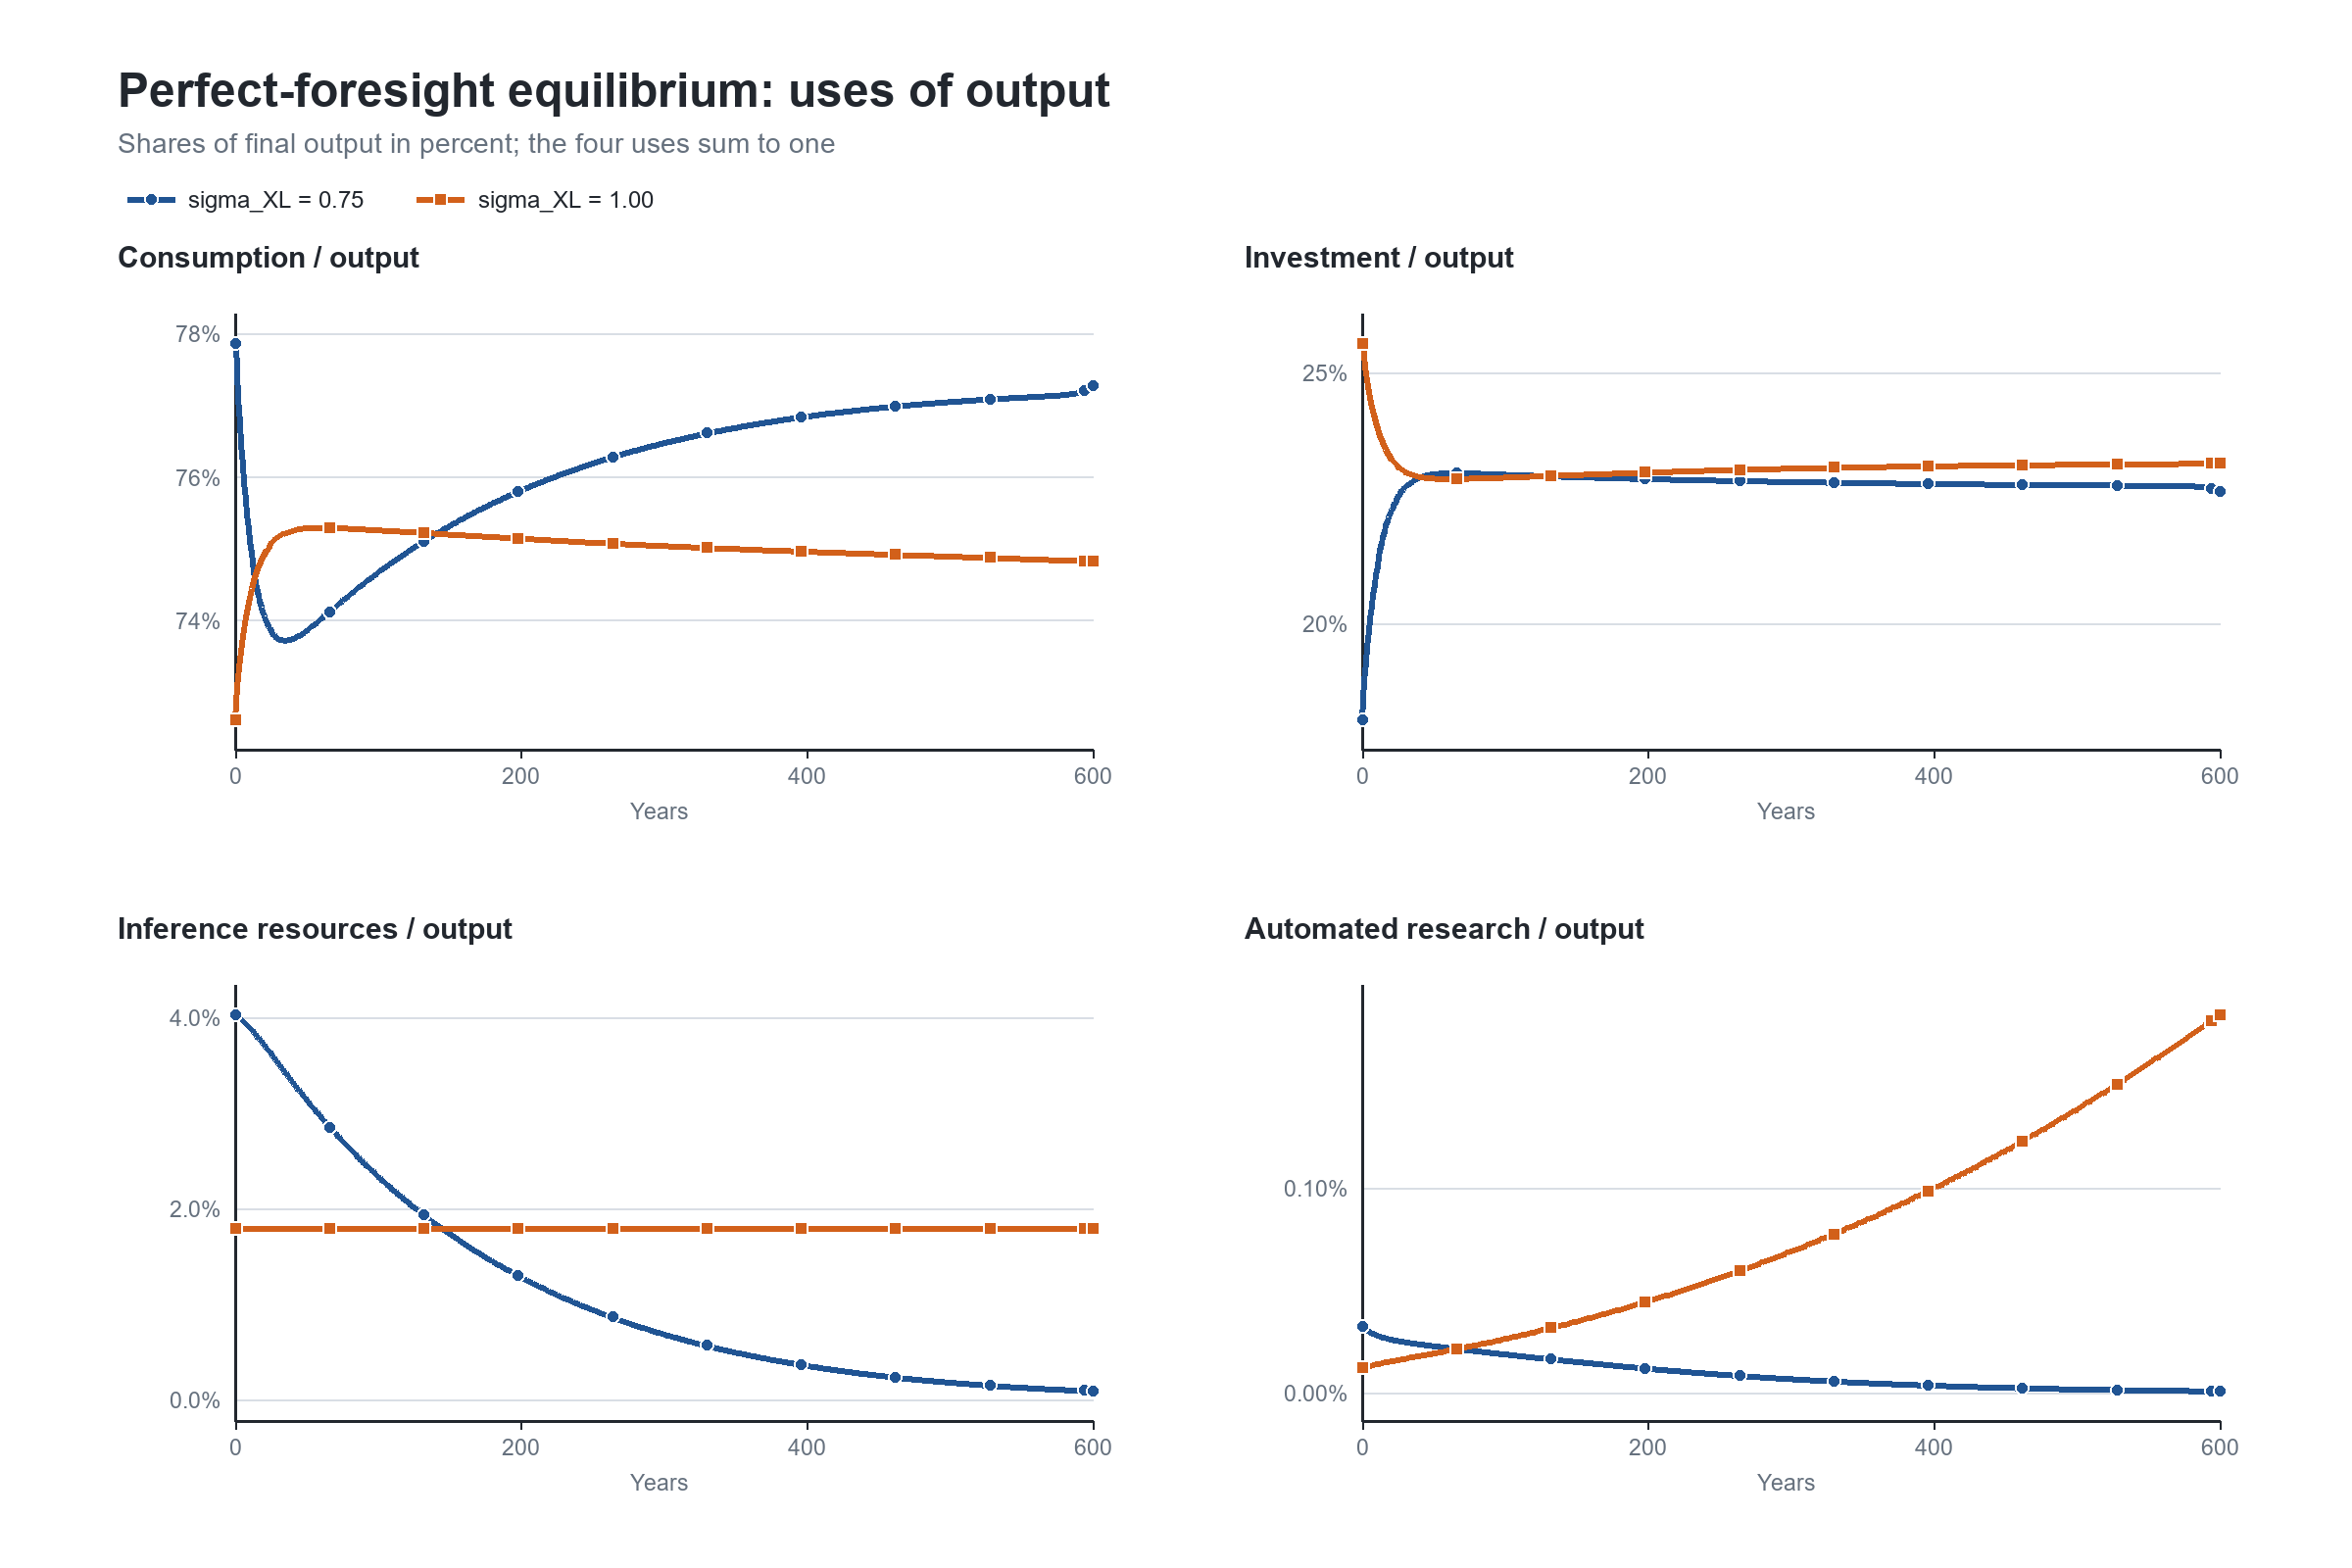
\includegraphics[width=\textwidth]{figures/equilibrium_resource_allocation.png}
    \caption{Equilibrium allocation of final output. The panels show $C/Y$,
    $I/Y$, $\xi U/Y$, and $\xi M/Y$ in percent.}
    \label{fig:equilibrium-resource-allocation}
\end{figure}

\begin{figure}[H]
    \centering
    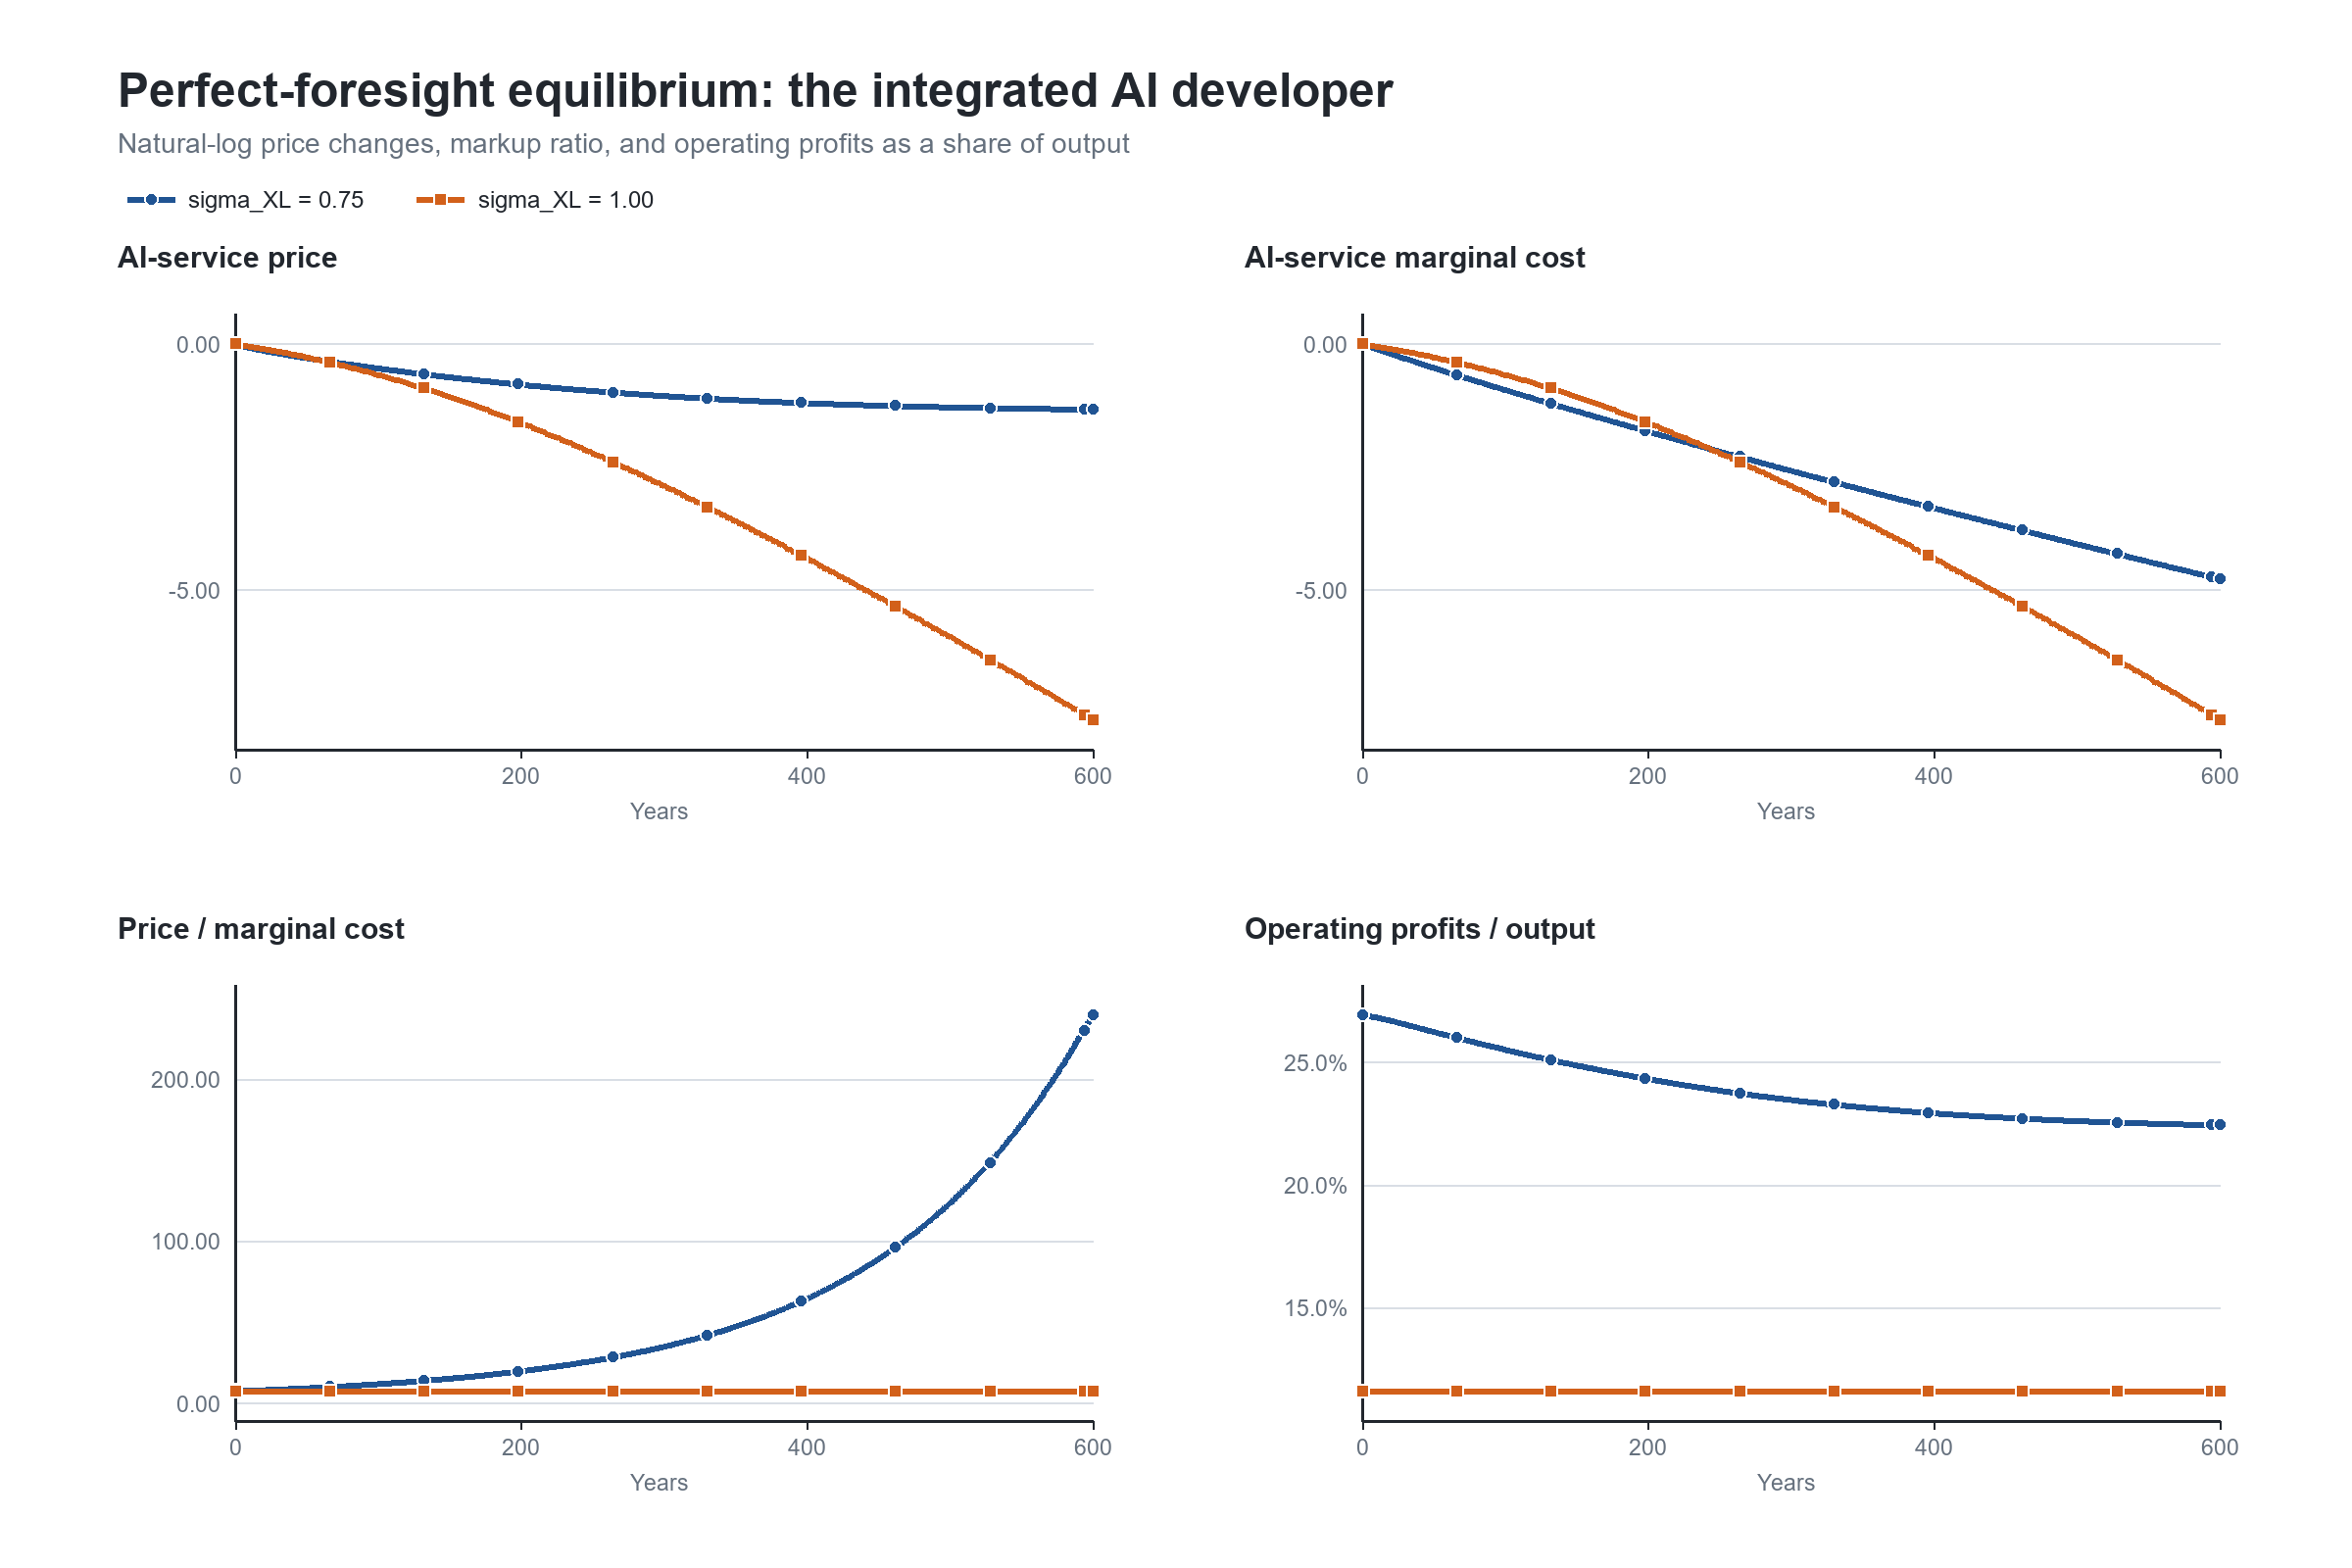
\includegraphics[width=\textwidth]{figures/equilibrium_monopoly_block.png}
    \caption{The integrated AI developer. Price and marginal cost are natural-log
    changes; the markup is the price--marginal-cost ratio and operating profits
    are reported as a share of output.}
    \label{fig:equilibrium-monopoly-block}
\end{figure}

\subsection{Case IV: production gross substitution, $\sigma_{XL}>1$}
\label{sec:case-production-substitutes}

\subsubsection{Analytical characterization}

Proposition~\ref{prop:gross-substitution-no-steady-state} rules out an interior
finite-rate steady state with positive capability growth. As capability lowers the
resource cost of AI services, an exact equilibrium lower bound makes $Y/K$ rise
without bound even without assuming a path for the endogenous AI expenditure
share. The return to capital and the growth rate implied by the Euler equation
therefore cannot converge to finite constants. If the normalized AI-service cost
also vanishes, the stronger result $s^X_t\to1$ follows. Conditional
result~\ref{cond:high-sigma-singular-scaling} goes further under its stated
AI-dominated scaling and characterizes a finite-time singular branch. The
nonexistence proposition does not by itself prove that the optimizing equilibrium
selects that branch; it may encounter an allocation boundary first.

\subsubsection{Free-boundary equilibrium transitions}

The core production-acceleration configuration uses $\sigma_{XL}=1.35$. The
$\sigma_{XL}=1.50$ and 2.00 paths check how substitution changes the timing of the
same regime. All three values lie below the static wage threshold $1/\alpha$. This restriction
makes the direct effect of an AI-service expansion on the wage positive, but does
not by itself determine the equilibrium wage path. The simulations verify that the
wage rises and automated research becomes asymptotically dominant. Table
\ref{tab:high-sigma-equilibrium-summary} reports the terminal boundary, the
endogenous time at which the path reaches it, and
\begin{equation}
    \widehat T^*
    =
    T+\frac{1}{\vartheta\bar a\,z_T},
    \label{eq:estimated-singularity-time}
\end{equation}
which follows from equation~\eqref{eq:high-sigma-time-to-singularity}. The final
column reports the smallest wage-growth rate along each path, not its terminal
value.

\begin{table}[htbp]
    \centering
    \caption{Free-boundary equilibrium paths with $\sigma_{XL}>1$}
    \label{tab:high-sigma-equilibrium-summary}
    \begin{tabular}{cccccc}
        \toprule
        $\sigma_{XL}$ & $z_T$ & $T$ & $\widehat T^*$
        & first year $g_{Y/N}\geq5\%$ & $\min_t g_w$ \\
        \midrule
        1.35 & 50  & 333.22 & 333.38 & 297 & 0.070\% \\
        1.50 & 50  & 280.29 & 280.45 & 247 & 0.054\% \\
        2.00 & 100 & 209.00 & 209.08 & 180 & 0.028\% \\
        \bottomrule
    \end{tabular}
    \begin{minipage}{0.96\textwidth}
    \footnotesize\emph{Notes:} Calendar time is measured from the common initial
    stocks. The dates are conditional on the illustrative parameter values in
    Table~\ref{tab:equilibrium-numerical-parameters}; they are not calibrated
    forecasts.
    \end{minipage}
\end{table}

Figure~\ref{fig:high-sigma-equilibrium-levels} shows a long interval of moderate
growth followed by a sharp acceleration. Moving $\sigma_{XL}$ from 1.35 to 2.00
brings the acceleration forward by more than a century. The comparison is not
generated by different investment or research-spending rules: the household and
the developer optimize along every path.

\begin{figure}[H]
    \centering
    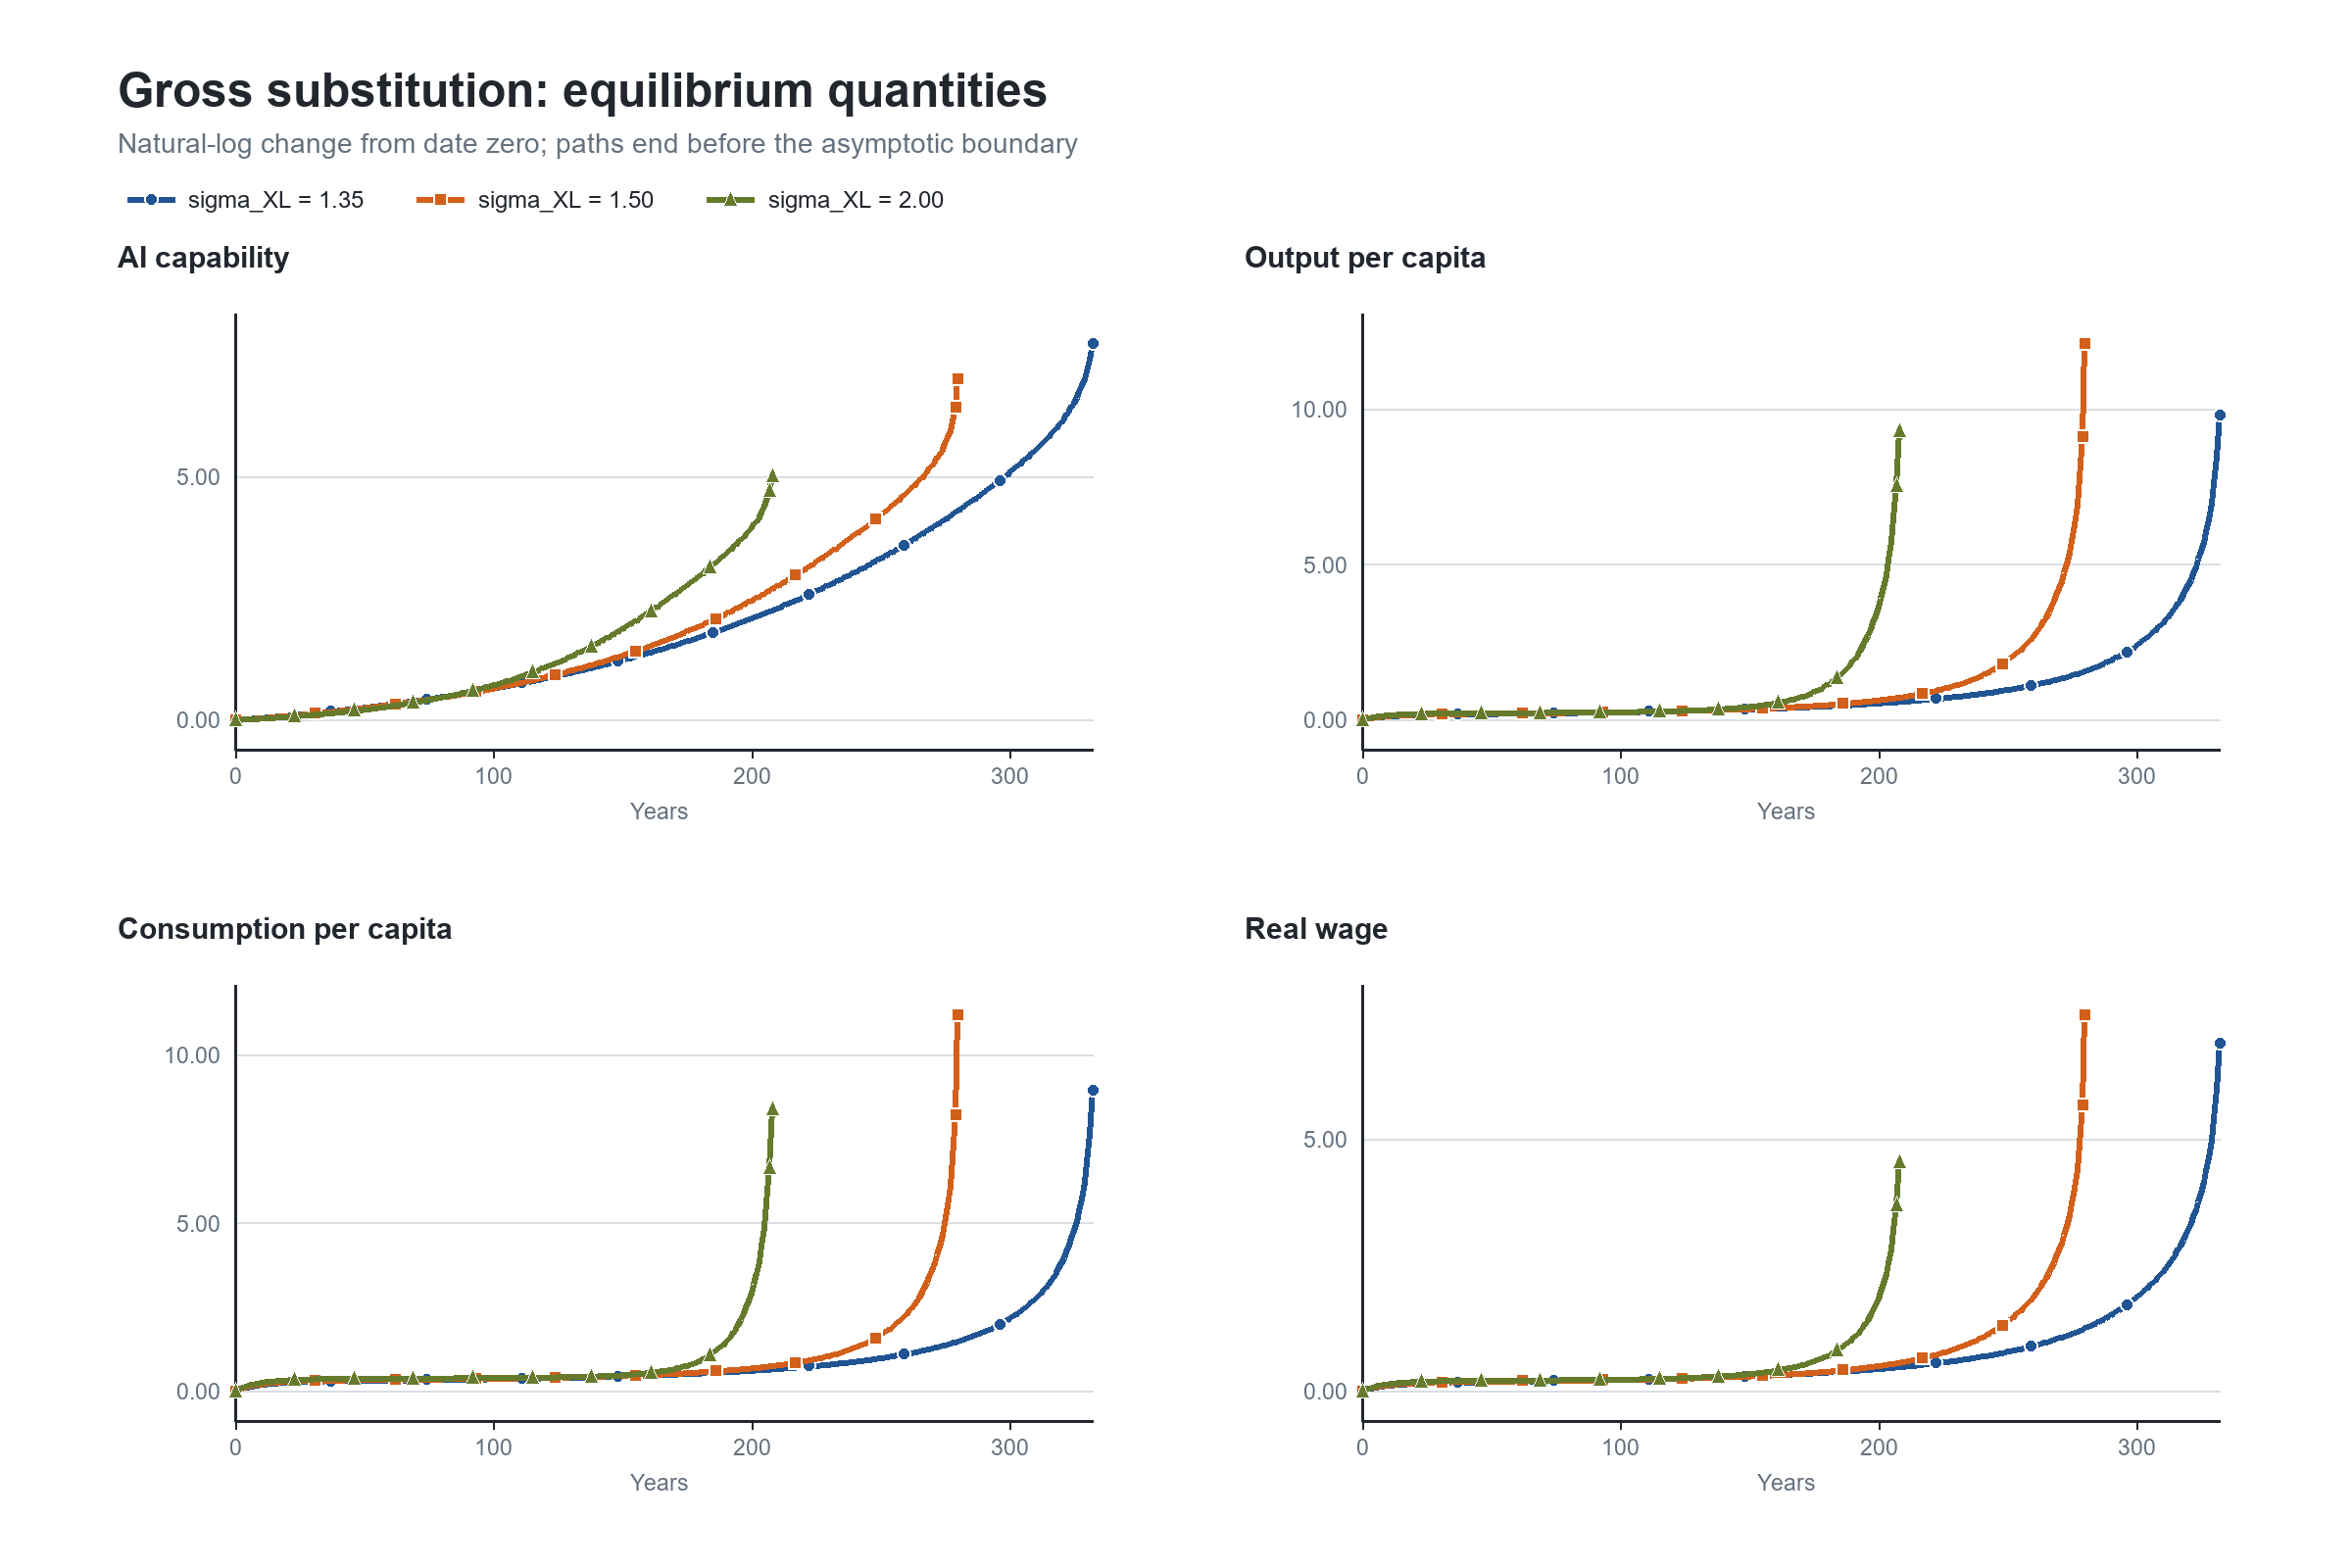
\includegraphics[width=\textwidth]{figures/high_sigma_equilibrium_levels.png}
    \caption{Equilibrium quantities with gross substitution. Each panel reports
    the natural-log change from the path's date-zero value. For
    comparability, the displayed paths end no later than $Y/K=20$.}
    \label{fig:high-sigma-equilibrium-levels}
\end{figure}

The production-chain panels in
Figure~\ref{fig:high-sigma-equilibrium-production-chain} show where the
acceleration originates. Capability growth lowers the marginal resource cost of
AI services, which induces a large expansion of inference compute and an even
larger expansion of AI services. The service composite consequently ceases to be
constrained by labor. The dates differ sharply across elasticities, but the ordering
of the mechanism is the same in all three equilibria.

\begin{figure}[H]
    \centering
    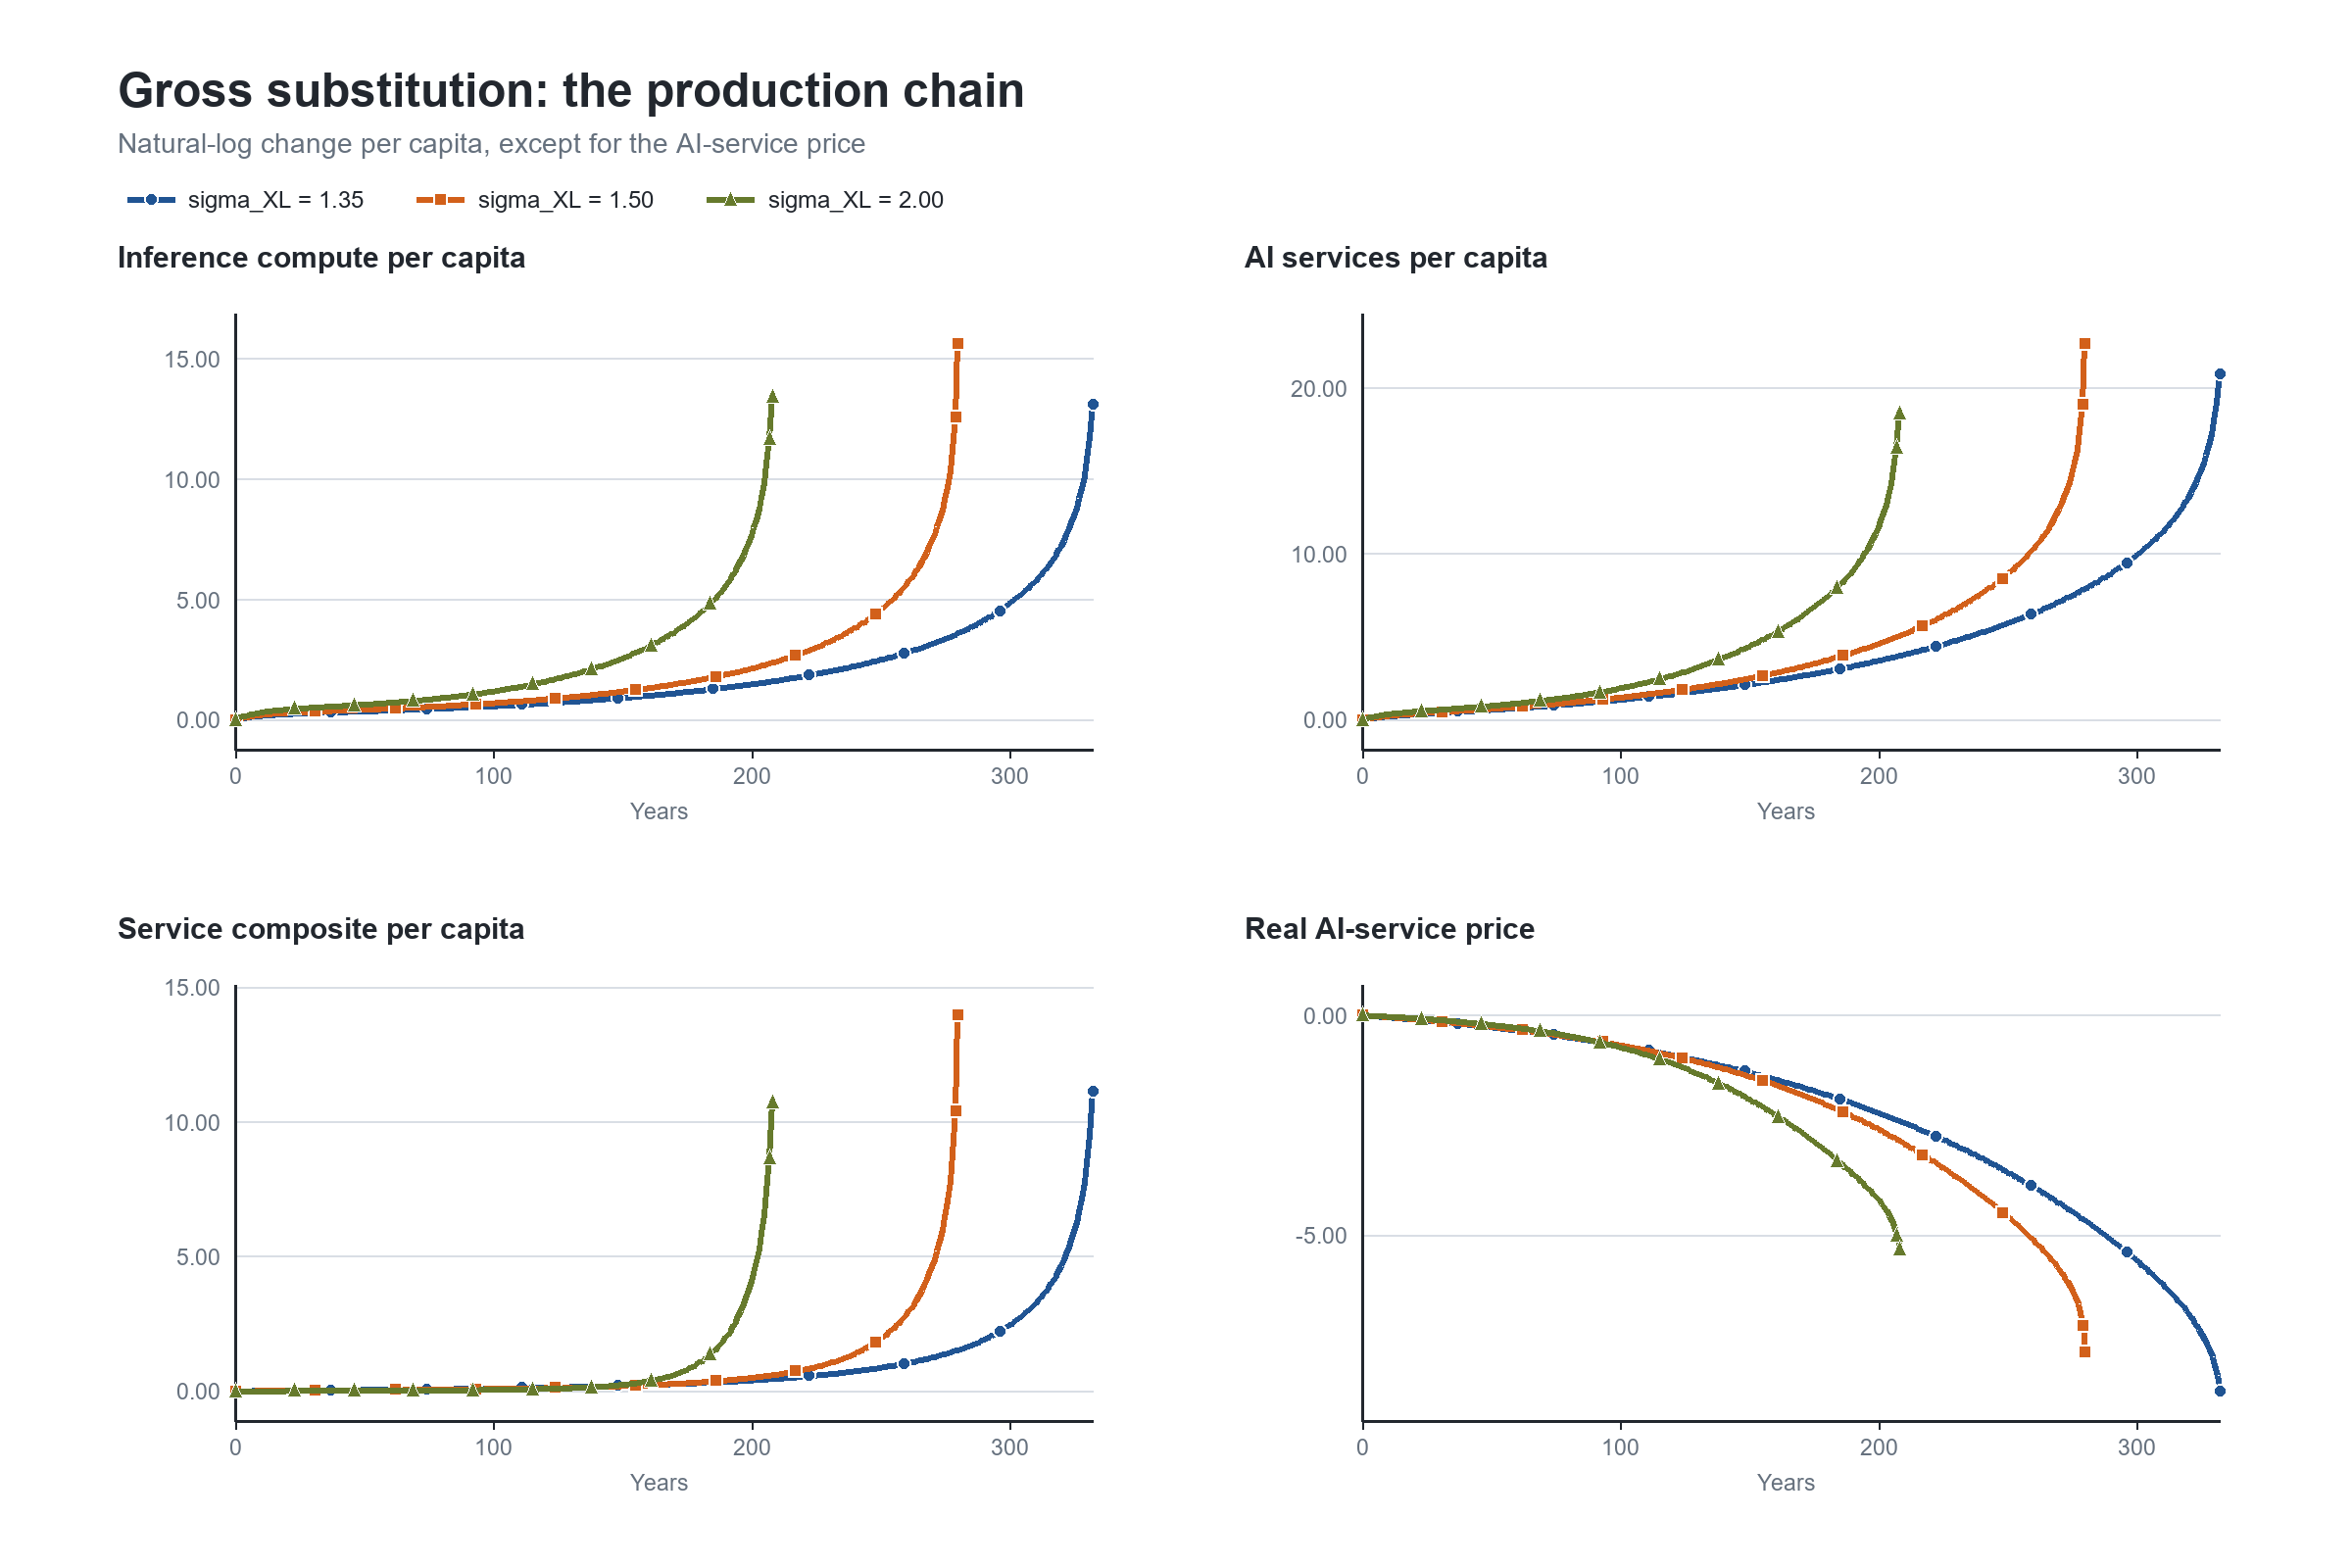
\includegraphics[width=\textwidth]{figures/high_sigma_equilibrium_production_chain.png}
    \caption{Production chain with gross substitution. Quantity panels report
    natural-log changes per capita and the price panel reports a natural-log
    change. Paths are displayed only up to $Y/K=20$.}
    \label{fig:high-sigma-equilibrium-production-chain}
\end{figure}

The growth rates and the return to capital in Figure
\ref{fig:high-sigma-equilibrium-growth} remain comparatively low through most of
the transition and then rise rapidly. Output-per-capita growth first exceeds 5
percent after 297 years when $\sigma_{XL}=1.35$, after 247 years when it is 1.50,
and after 180 years when it is 2.00. The real wage rises throughout all three
paths. The acceleration therefore does not require a falling wage, even though
labor receives a vanishing share of output.

Figure~\ref{fig:high-sigma-equilibrium-monopoly-block} adds the objects that
cannot be inferred from quantities alone. Both the AI-service price and marginal
cost fall, and their decline accelerates. Unlike the complementarity case, the
price moves toward marginal cost: the markup declines toward roughly 1.5 on the
reported boundaries. Operating profits nevertheless rise from a small initial
share to about 22 percent of output. A lower markup can therefore coexist with a
larger aggregate profit share when the AI-service expenditure share expands.
These are equilibrium outcomes for the reported parameterization, not general
comparative-static propositions.

\begin{figure}[H]
    \centering
    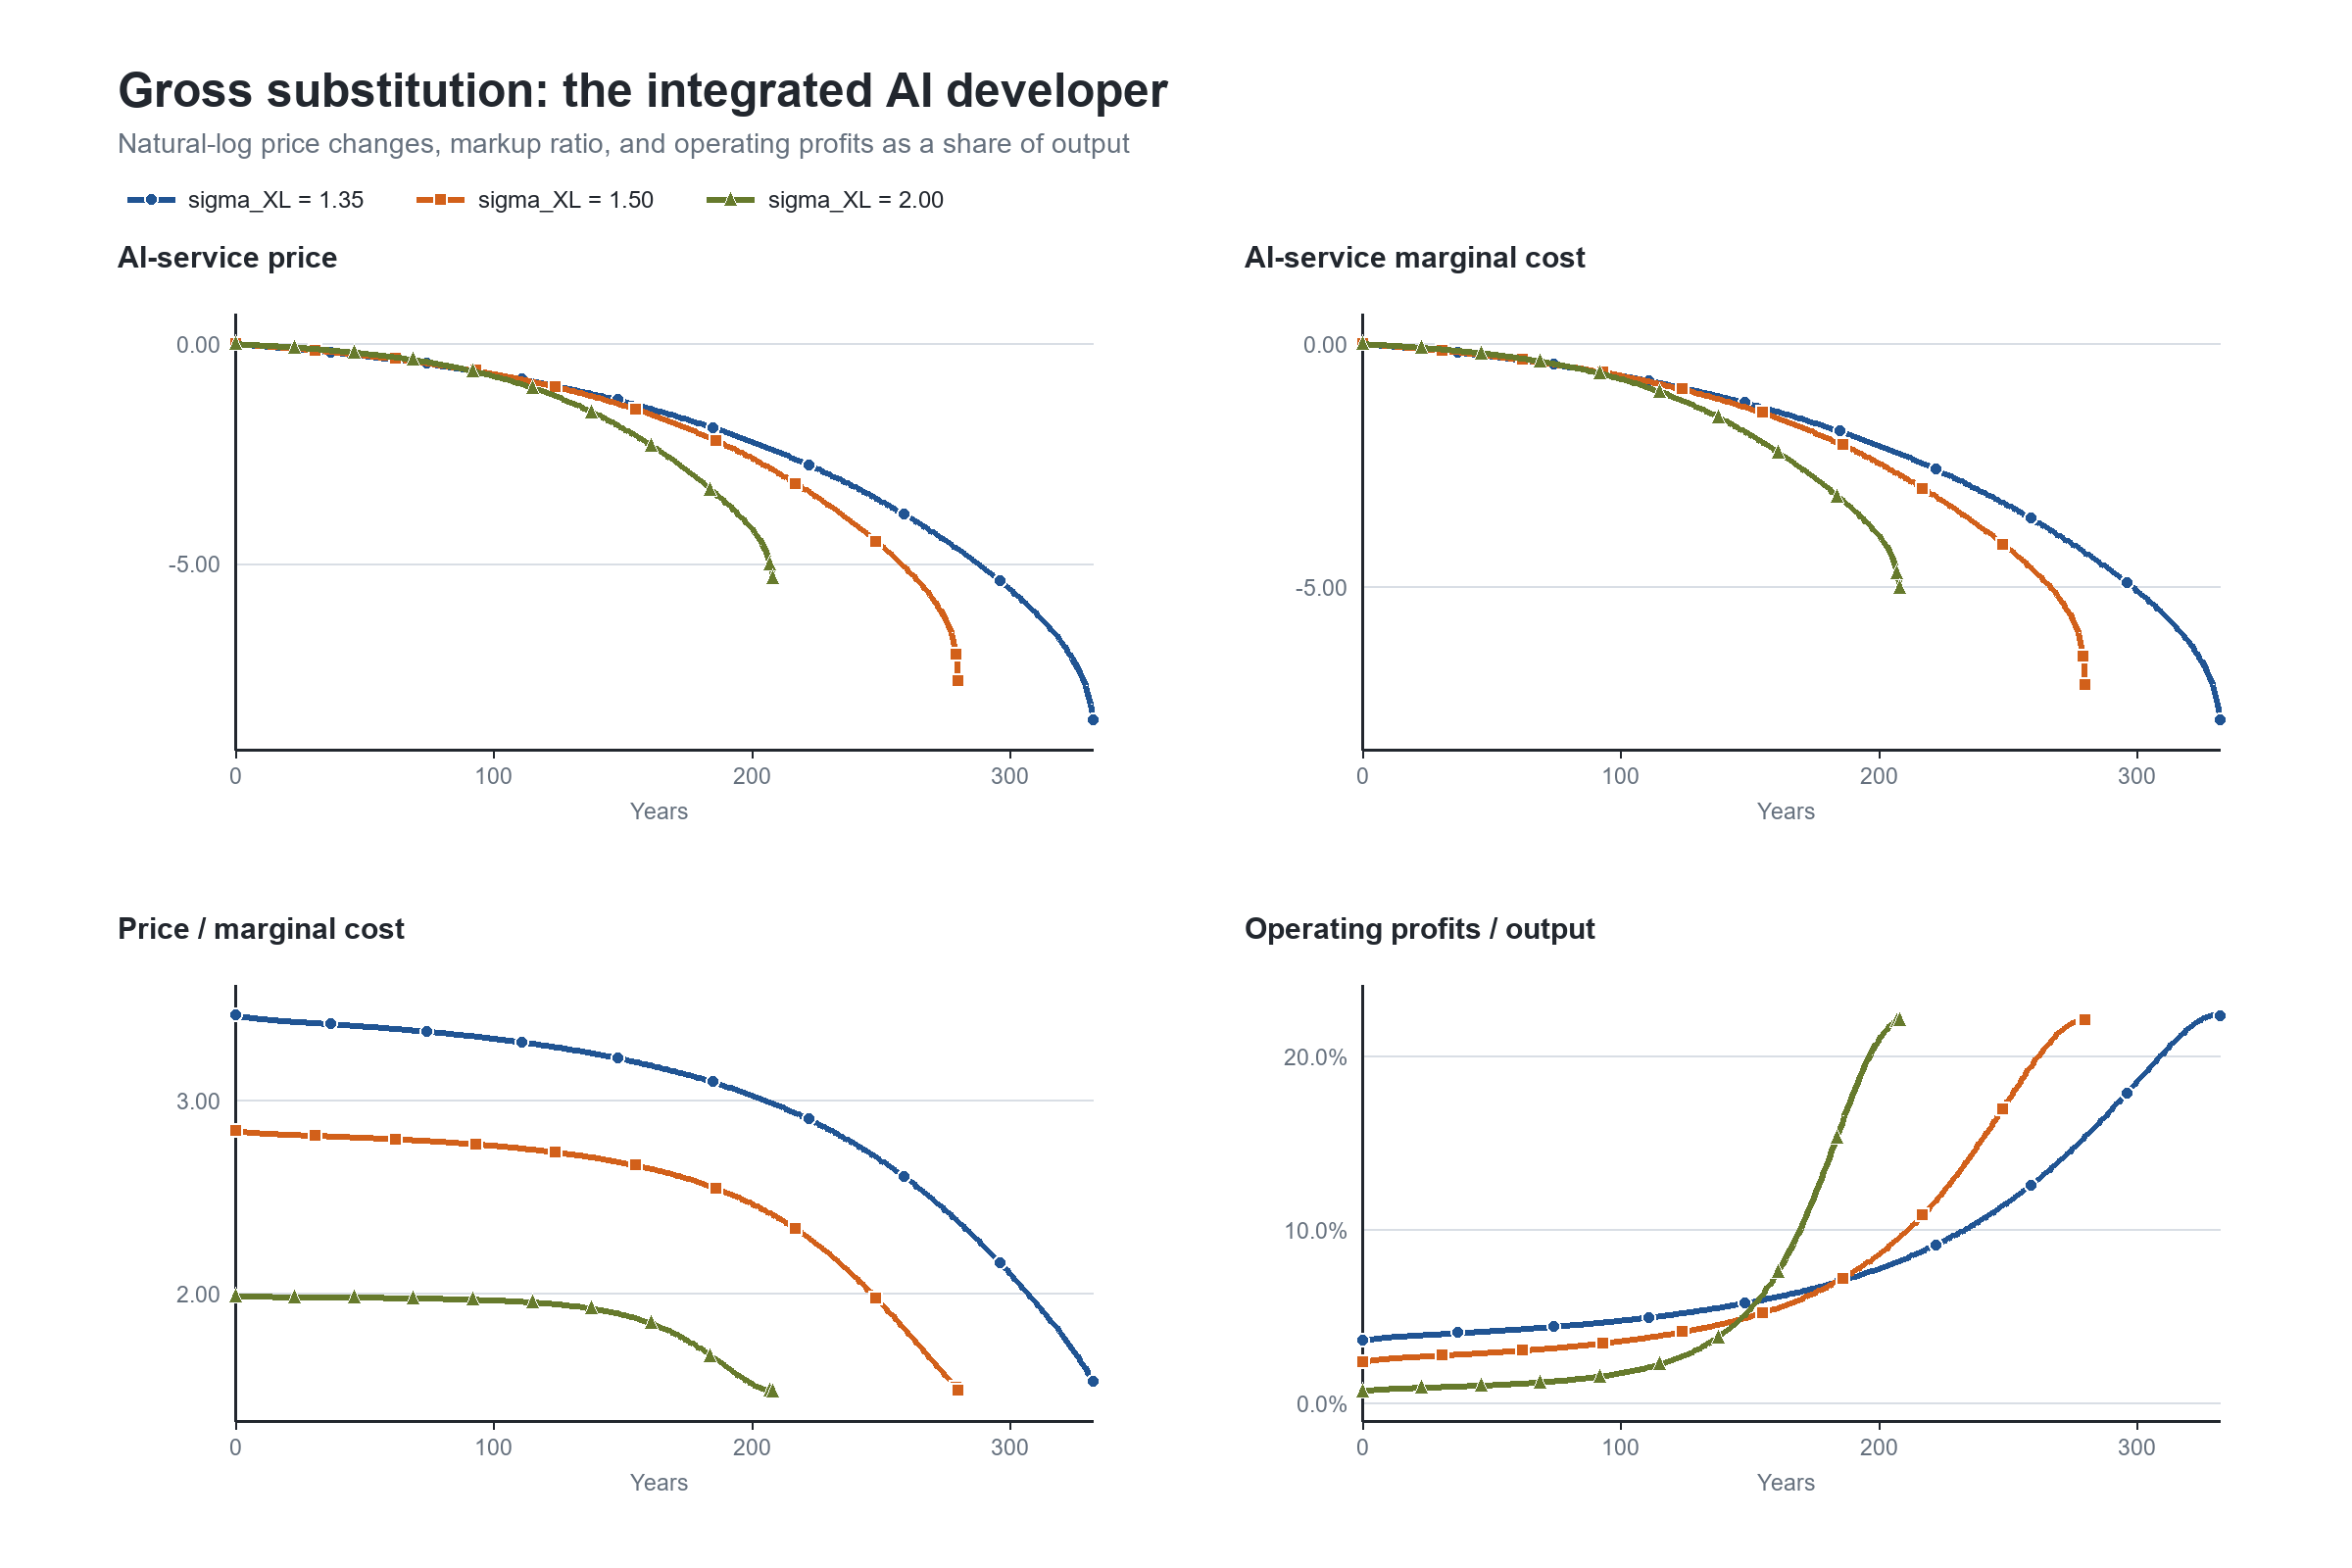
\includegraphics[width=\textwidth]{figures/high_sigma_equilibrium_monopoly_block.png}
    \caption{The integrated AI developer under gross substitution. Price and
    marginal cost are natural-log changes; the markup is a ratio and operating
    profits are a percentage of output.}
    \label{fig:high-sigma-equilibrium-monopoly-block}
\end{figure}

Figure~\ref{fig:high-sigma-equilibrium-shares} separates the production and
research margins. The AI contribution to production and the automated contribution
to research approach one, while the aggregate labor share approaches zero. Human
research employment need not follow the aggregate labor share. With
$\sigma_{XL}=1.35$ and 1.50, $H/N$ rises and later falls as automated research
becomes dominant. With $\sigma_{XL}=2$, the scale of research expands so quickly
that $H/N$ reaches 90.7 percent at the $Y/K=100$ boundary even though automated
systems account for 99.8 percent of effective research. A nearly automated research
technology can therefore employ most humans while paying them a negligible share
of an economy that is growing much faster than wages.

\begin{figure}[H]
    \centering
    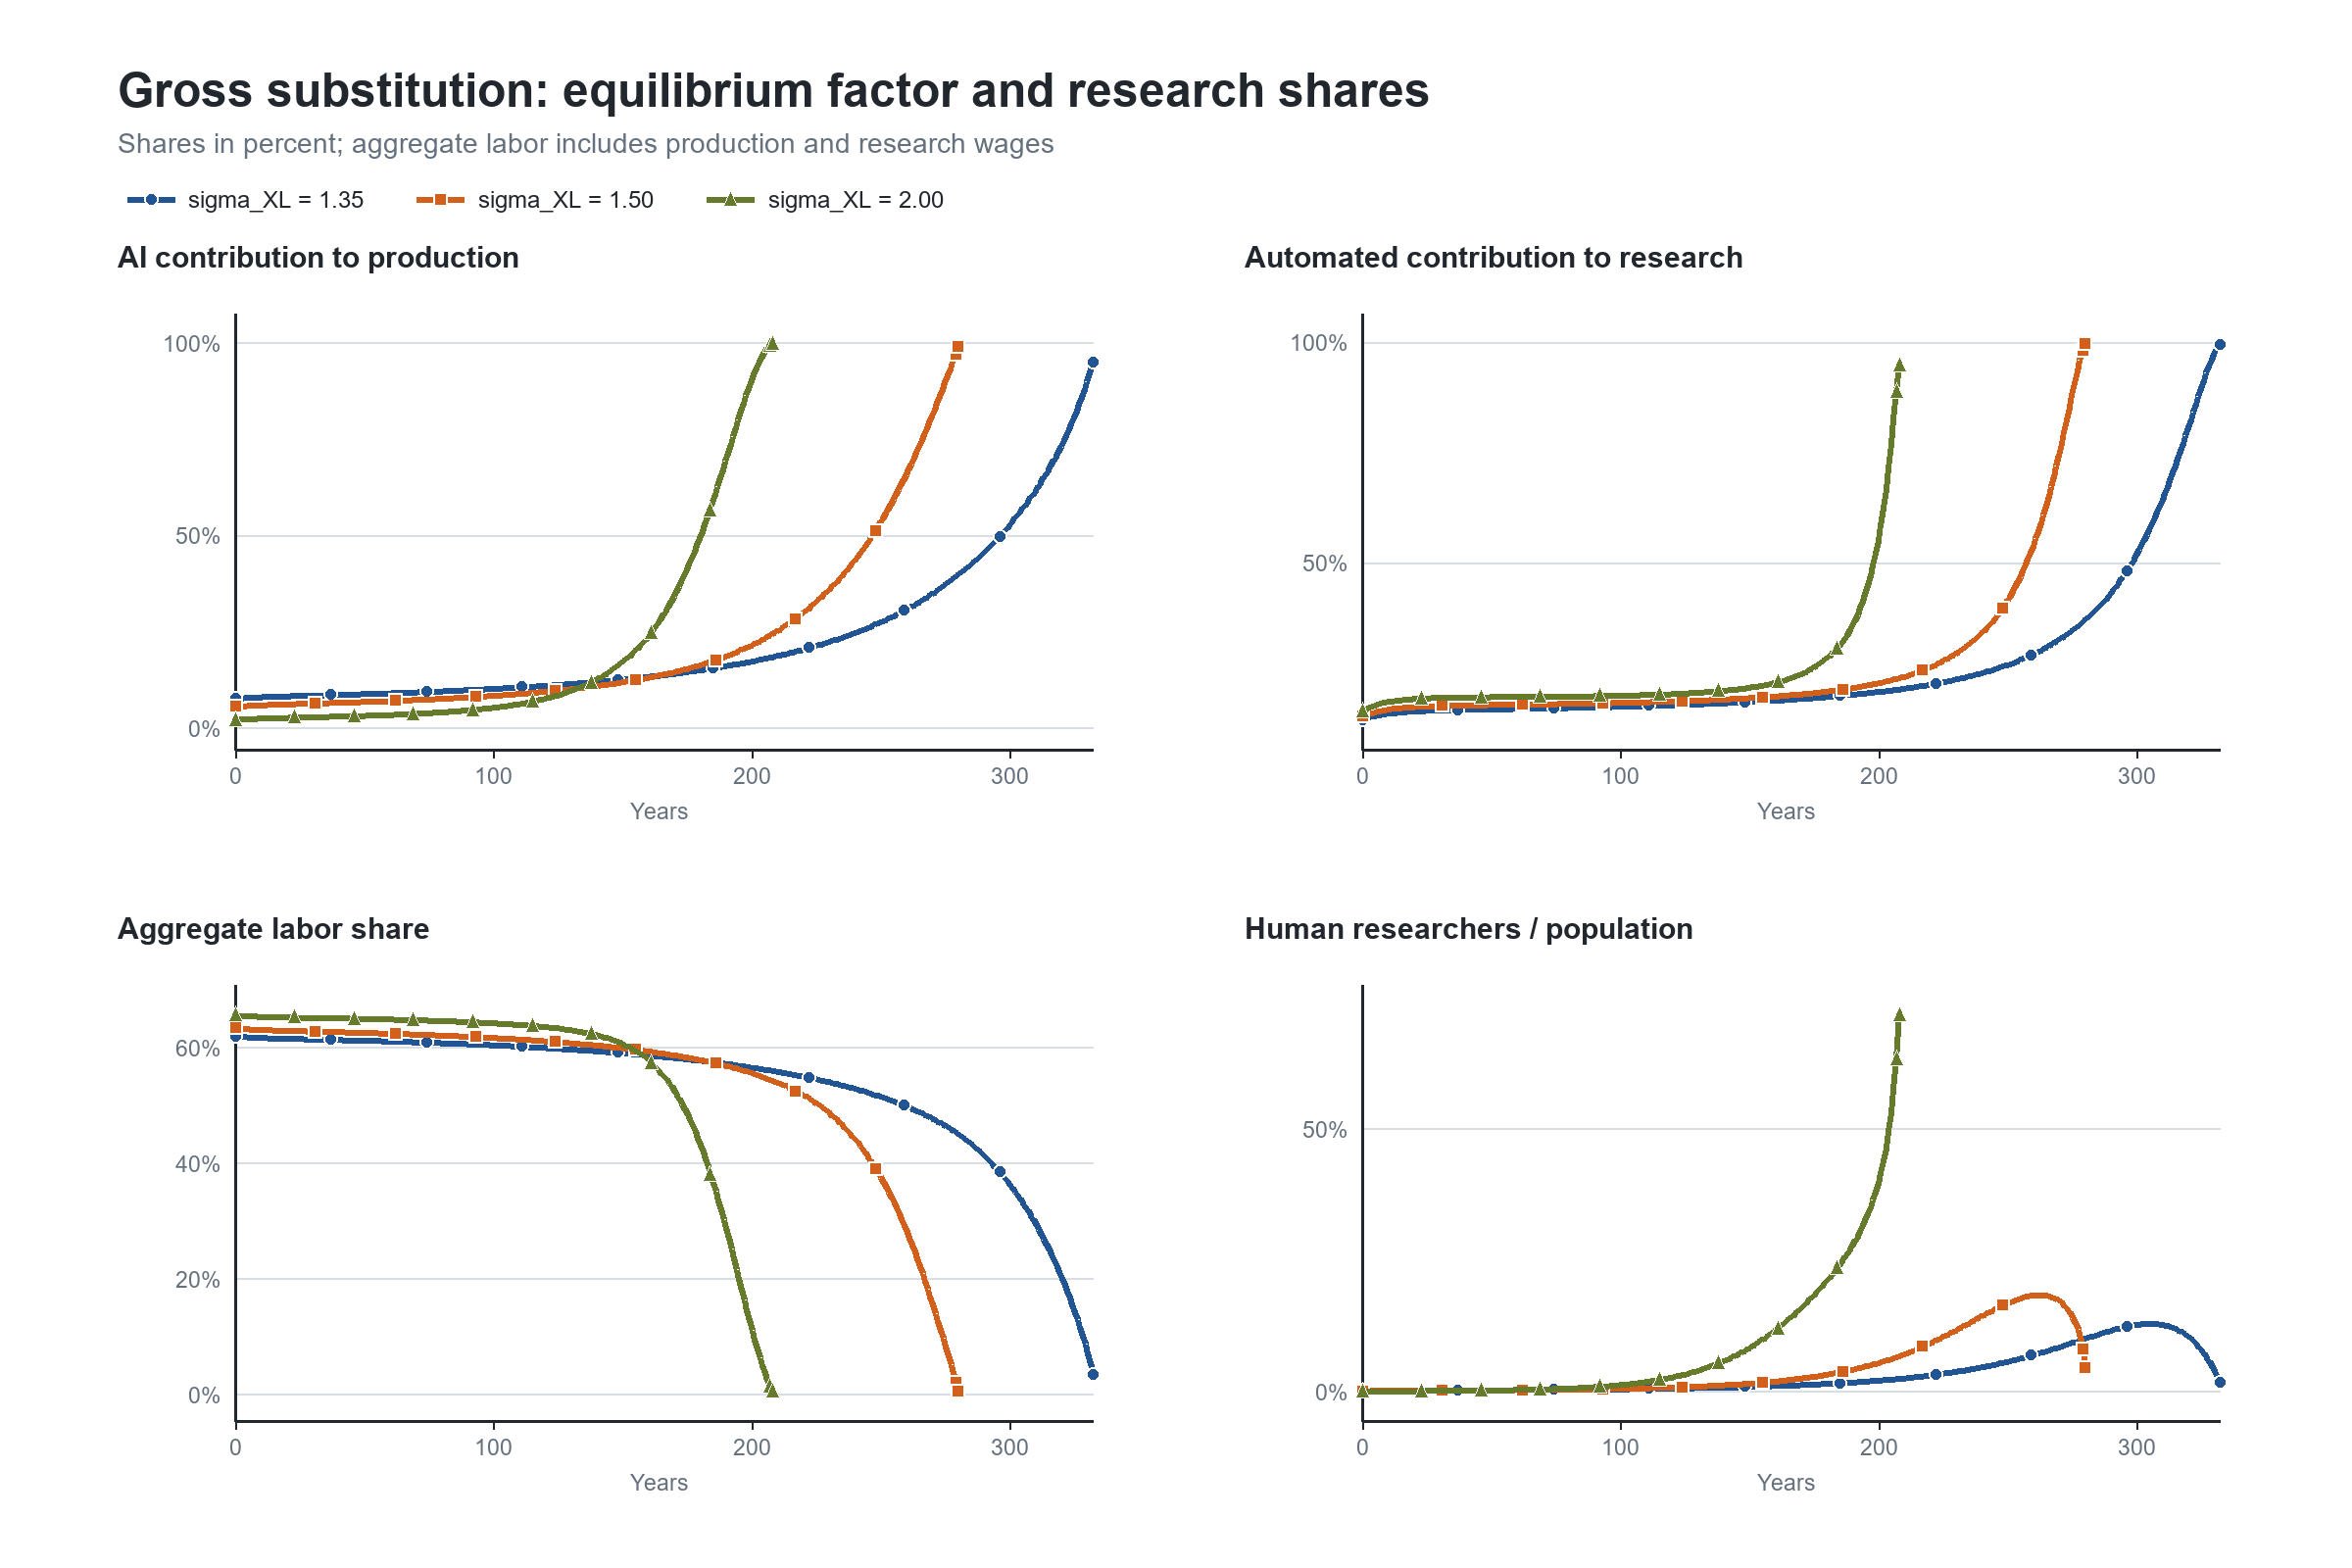
\includegraphics[width=\textwidth]{figures/high_sigma_equilibrium_shares.png}
    \caption{Production, research, and labor allocation along the gross-substitution
    equilibria. The aggregate labor share includes production and research wages.}
    \label{fig:high-sigma-equilibrium-shares}
\end{figure}

Figure~\ref{fig:high-sigma-equilibrium-research-chain} complements those shares
with levels. Automated and effective research expand rapidly per capita, while
$\ln(H/M)$ falls without reversal. Human research per capita can first rise and
then fall, or keep rising over the computed interval, because its level reflects
both a declining human intensity and an expanding research sector. This is the
numerical counterpart of Proposition~\ref{prop:research-employment-scale}.

\begin{figure}[H]
    \centering
    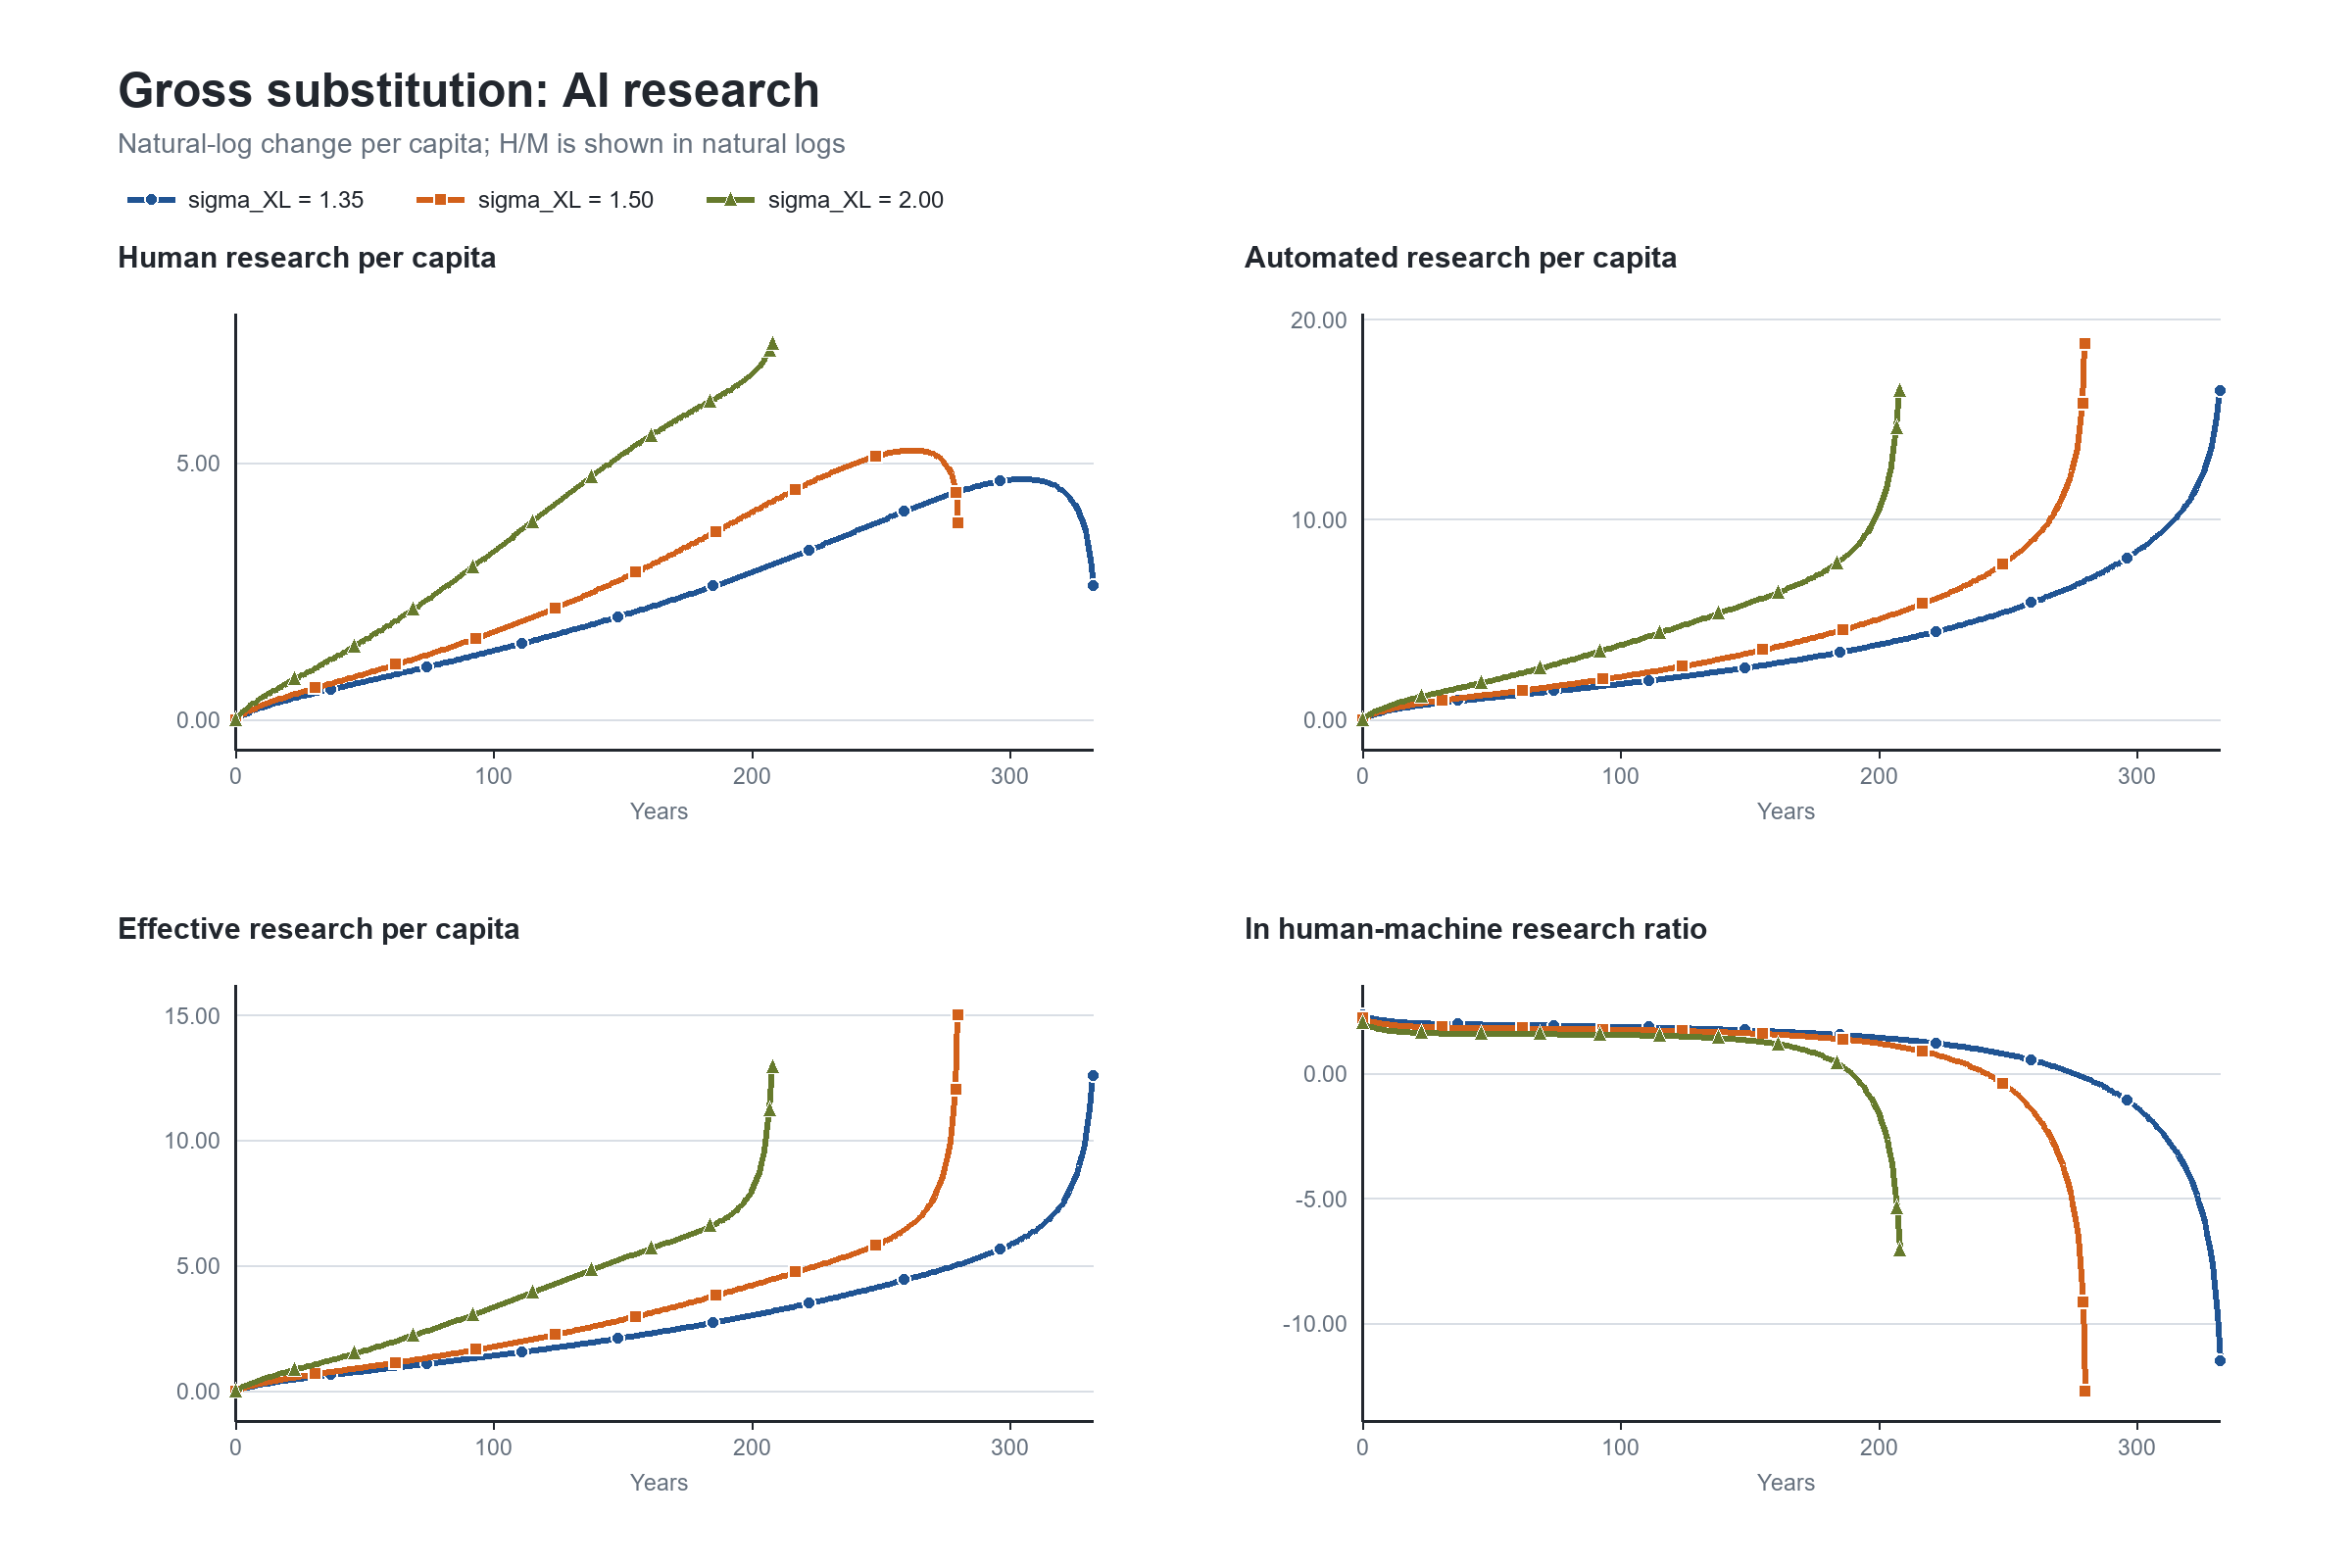
\includegraphics[width=\textwidth]{figures/high_sigma_equilibrium_research_chain.png}
    \caption{Research chain with gross substitution. The first three panels
    report natural-log changes per capita; the final panel reports $\ln(H/M)$.}
    \label{fig:high-sigma-equilibrium-research-chain}
\end{figure}

The resource allocation in
Figure~\ref{fig:high-sigma-equilibrium-resource-allocation} shows that acceleration
is accompanied by a large reallocation of output. Inference absorbs close to 45
percent of output at the terminal boundaries and automated research about 8--9
percent, while consumption falls toward the imposed limiting share. Investment
does not vanish: it remains near 20 percent of output. These shares satisfy the
resource constraint at every plotted date.

\begin{figure}[H]
    \centering
    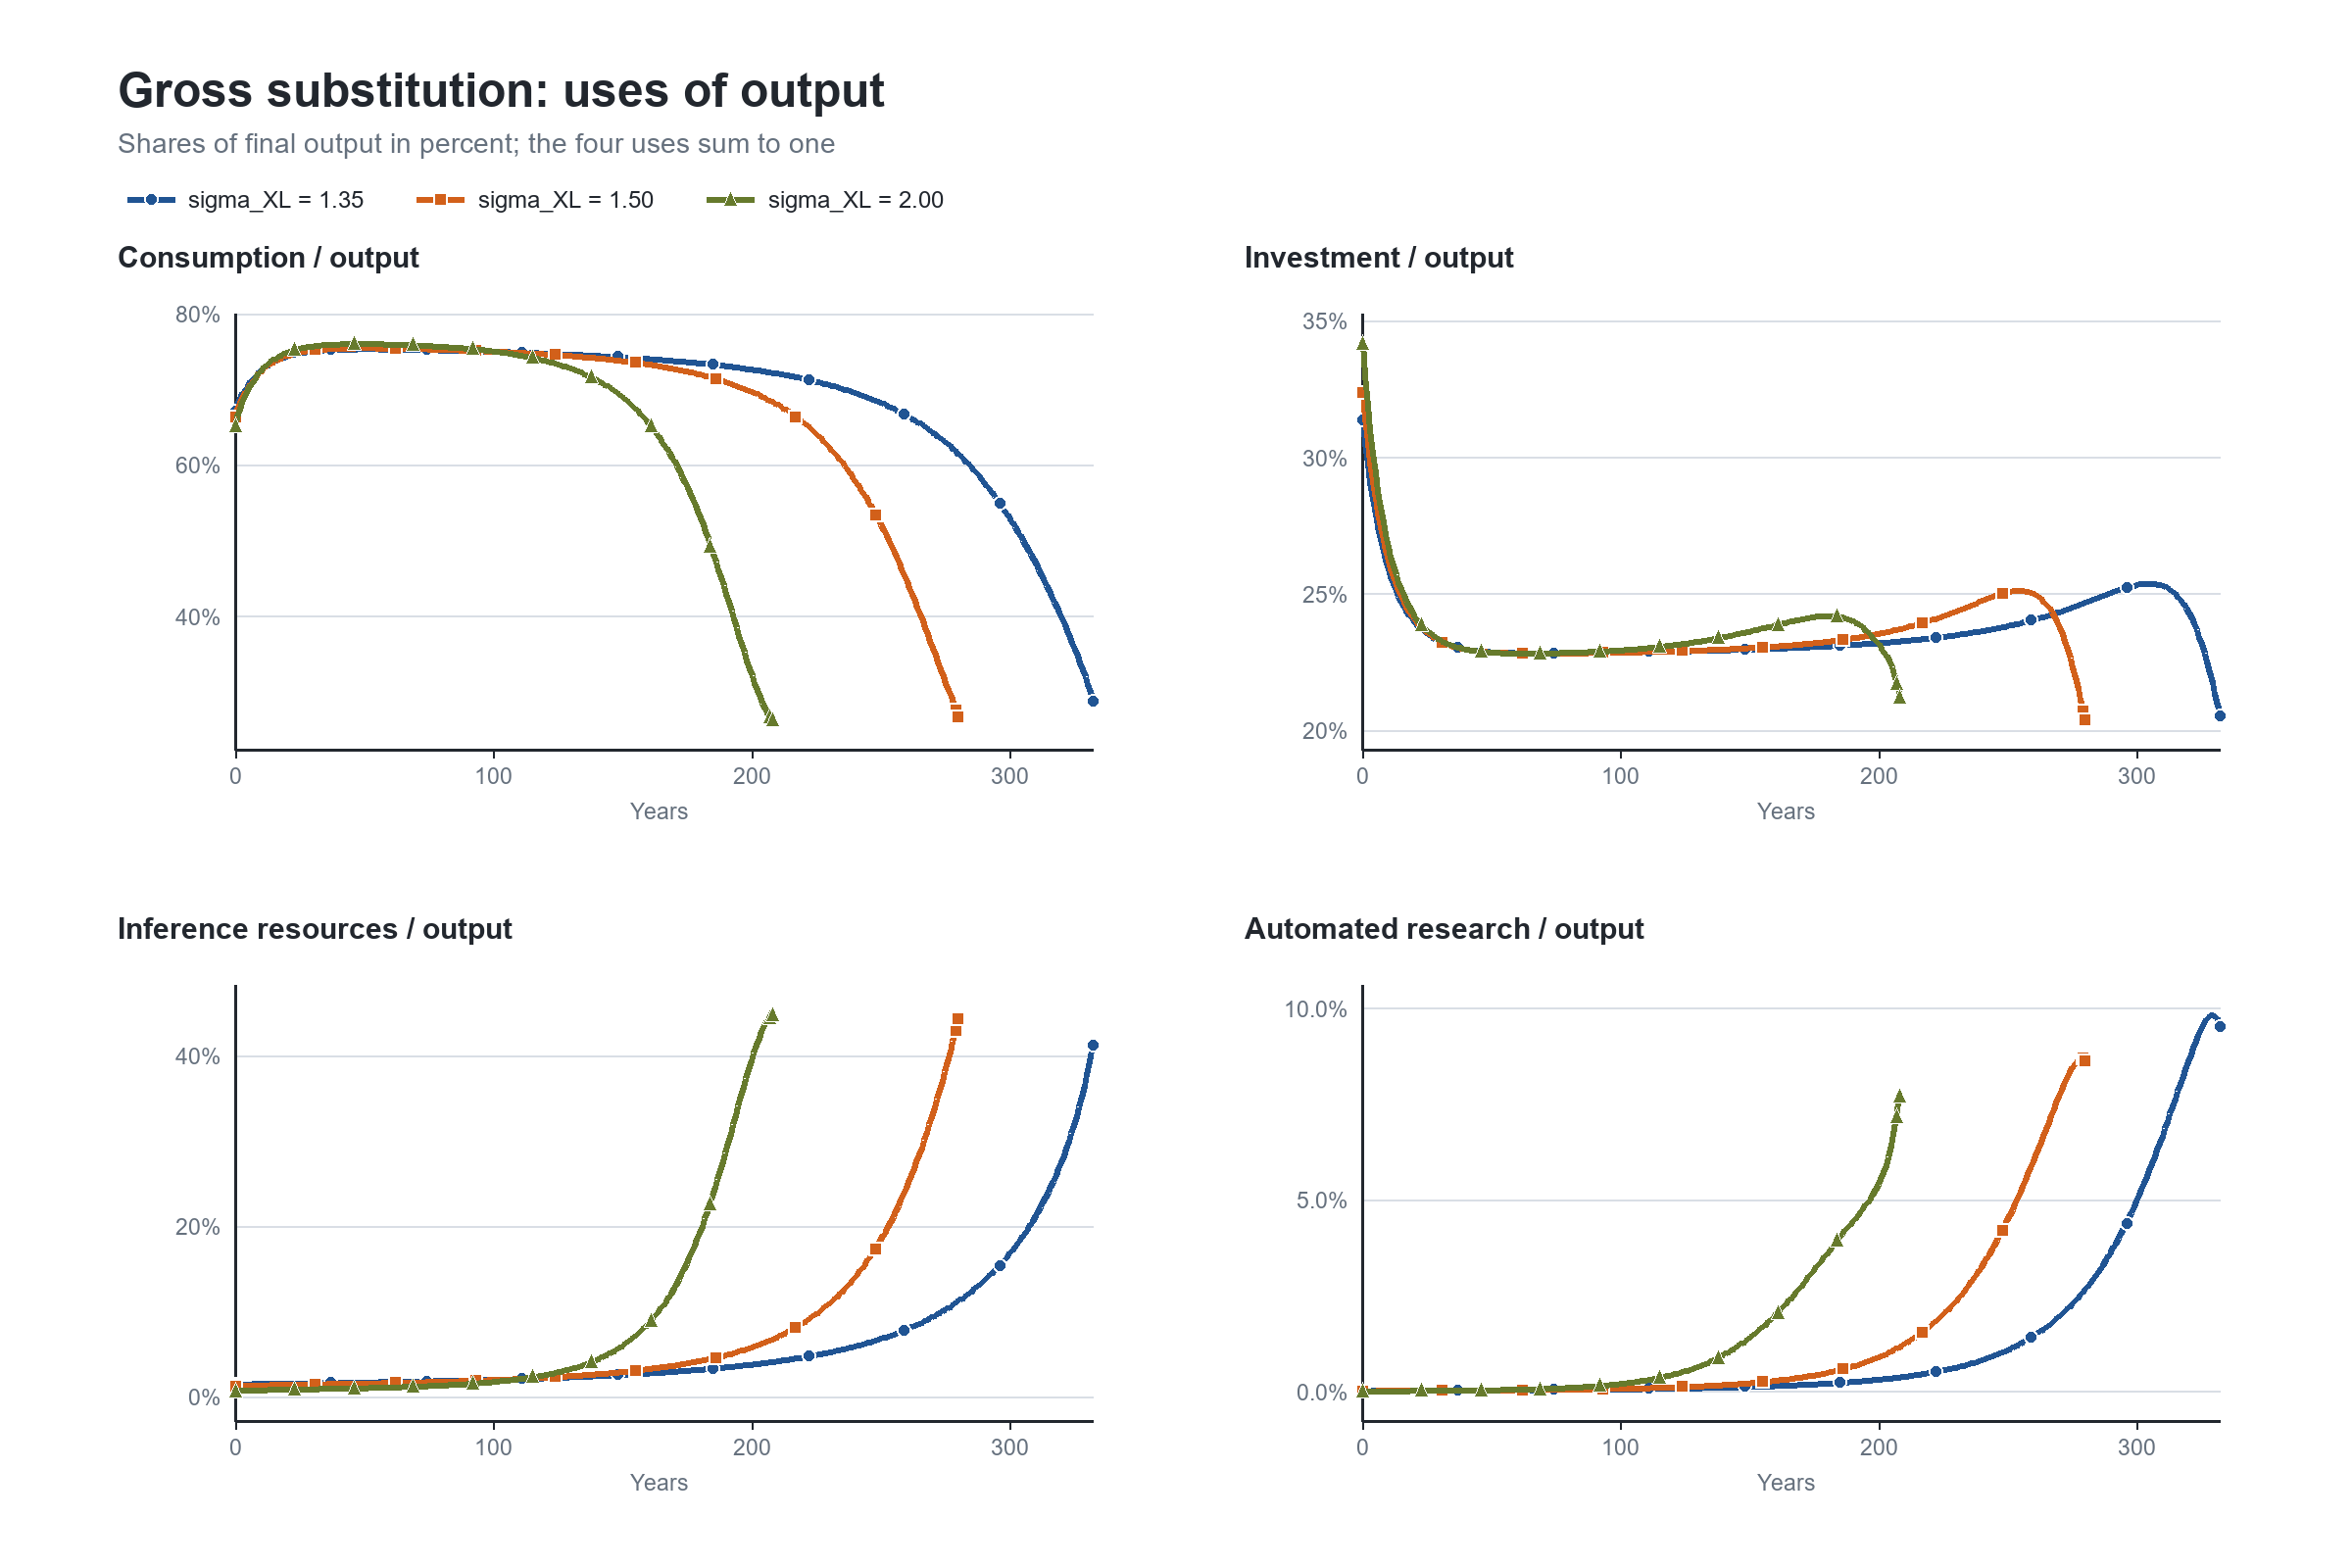
\includegraphics[width=\textwidth]{figures/high_sigma_equilibrium_resource_allocation.png}
    \caption{Allocation of output along the gross-substitution equilibria. Each
    panel is a percentage of final output; the four shares add to one.}
    \label{fig:high-sigma-equilibrium-resource-allocation}
\end{figure}

The boundary tests show that the terminal condition is not driving the transition.
Moving $z_T$ from 20 to 50 changes $\widehat T^*$ from 333.343 to 333.379 years
when $\sigma_{XL}=1.35$ and from 280.436 to 280.450 years when it is 1.50. For
$\sigma_{XL}=2$, moving $z_T$ from 20 to 50 and then to 100 changes
$\widehat T^*$ from 209.079 to 209.076 and 209.075 years. Across these sequences,
initial log consumption changes by less than $2.1\times10^{-8}$ and the initial log
shadow value by less than $3.0\times10^{-5}$.

The boundary directly imposes $C/Y=26.29$ percent and the limiting value of
$qA/K$. Those two ratios are therefore not independent numerical tests of
conditional result~\ref{cond:high-sigma-singular-scaling}. The non-imposed ratio
$g_A/(Y/K)$ approaches its theoretical value of 0.0624. At the largest boundaries,
the investment shares lie between 20.43 and 20.49 percent, compared with the
predicted 20.33 percent, while automated-research resource shares lie between 8.38
and 9.00 percent, compared with the predicted 8.49 percent. These independent
objects provide the relevant numerical check of the singular scaling.

\begin{figure}[H]
    \centering
    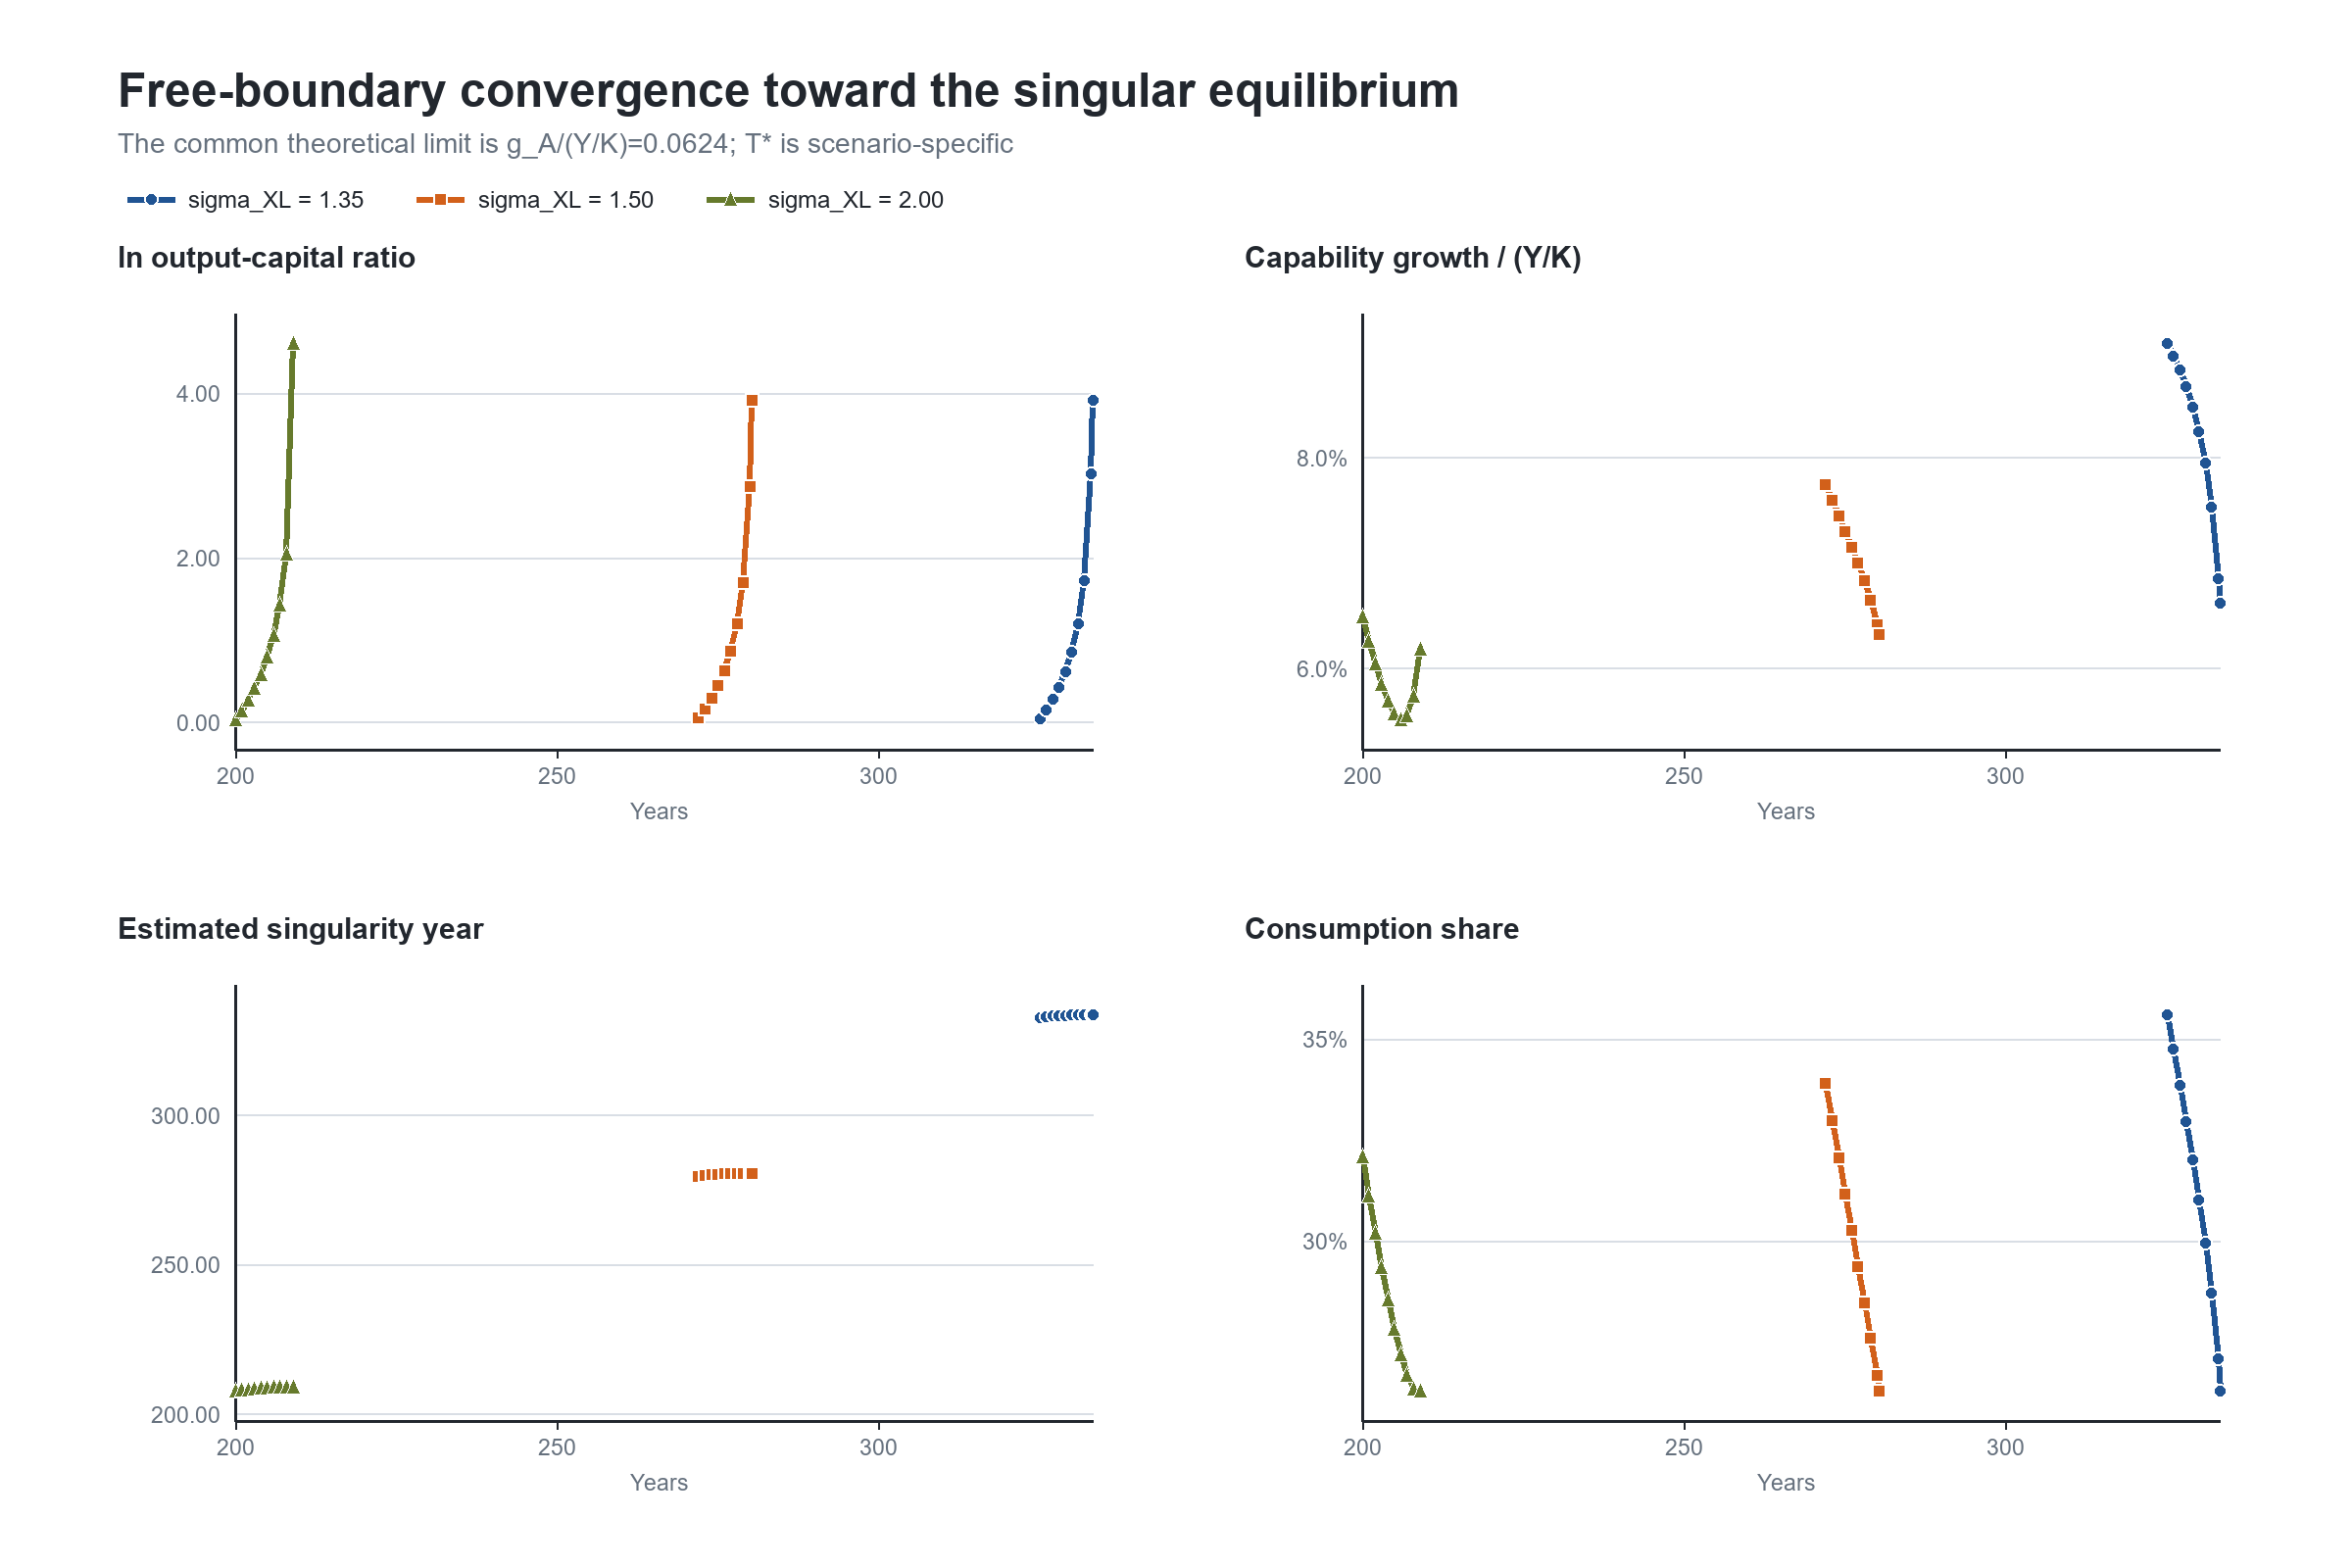
\includegraphics[width=\textwidth]{figures/high_sigma_equilibrium_asymptotics.png}
    \caption{Convergence toward the conditional singular-equilibrium ratios. The
    singularity-date estimator is evaluated only after $Y/K$ reaches one. The
    terminal consumption share is imposed by the free-boundary condition and is
    shown to describe the transition, not as an independent validation moment.}
    \label{fig:high-sigma-equilibrium-asymptotics}
\end{figure}

The maximum collocation residual across the three high-substitution solutions is
$3.0\times10^{-5}$. The largest equation-specific dynamic residual is
$1.7\times10^{-5}$, and the largest static first-order-condition residual is below
$2.0\times10^{-10}$. Labor-market clearing and the aggregate resource constraint
hold to machine precision. These checks establish that the reported curves solve
the numerical equilibrium system on their finite domains. They do not prove global
existence or uniqueness of the limiting singular path.

\subsubsection{Conditional wage-decline search above the static threshold}

The three preceding paths lie below $1/\alpha$, the threshold at which an expansion
of AI services lowers the wage when capital and production labor are held fixed. To
investigate whether the general-equilibrium wage can fall, we extend the numerical
search to $\sigma_{XL}>1/\alpha$ and allow population growth to rise above the
baseline value. Every reported path solves the household Euler equation, the
developer's first-order and costate conditions, the labor market, and the resource
constraint. However, conditional
result~\ref{cond:high-sigma-singular-scaling} establishes the AI-dominated terminal
ratios only for $1<\sigma_{XL}<1/\alpha$. Using those ratios above $1/\alpha$ is an
extrapolative boundary condition. The resulting objects are therefore conditional
equilibrium-branch searches on finite domains, not proofs of global existence or
selection of the terminal branch.

Table~\ref{tab:wage-decline-equilibrium-search} separates three wage outcomes. A
negative minimum value of $g_w$ establishes that the wage falls during part of the
transition. The peak-to-trough decline measures the cumulative fall from the wage's
previous maximum. The final column compares the trough with the wage at date zero.
These measures distinguish a temporary decline from a collapse of the wage level.

\begin{table}[htbp]
    \centering
    \caption{Conditional equilibrium-branch search for wage declines}
    \label{tab:wage-decline-equilibrium-search}
    \begin{tabular}{cccccc}
        \toprule
        $\sigma_{XL}$ & $n$ & $z_T$ & $\min_t g_w$
        & peak--trough decline & trough relative to $w_0$ \\
        \midrule
        4.00 & 1.2\% & 3  &  0.026\% & 0.00\% & 0.00\% \\
        5.00 & 3.0\% & 3  & $-0.216\%$ & 2.22\% & 28.04\% \\
        6.20 & 3.0\% & 10 & $-0.626\%$ & 7.68\% & 21.24\% \\
        6.28 & 3.9\% & 50 & $-0.800\%$ & 9.39\% & 16.72\% \\
        \bottomrule
    \end{tabular}
    \begin{minipage}{0.96\textwidth}
    \footnotesize\emph{Notes:} Except for $\sigma_{XL}$ and $n$, the paths use the
    common parameters and initial stocks in
    Table~\ref{tab:equilibrium-numerical-parameters}. The peak--trough decline is
    reported as a positive percentage. A positive value in the last column means
    that the trough remains above the date-zero wage. Population growth remains
    below the household discount rate, $\rho=4$ percent.
    \end{minipage}
\end{table}

The selected branches produce temporary wage declines but no wage collapse. The wage never falls
when $\sigma_{XL}=4$ and $n=1.2$ percent. When $\sigma_{XL}=5$ and $n=3$ percent,
wage growth becomes negative and the wage falls 2.22 percent from its previous peak.
The decline reaches 7.68 percent when $\sigma_{XL}=6.2$ and 9.39 percent when
$\sigma_{XL}=6.28$ and $n=3.9$ percent. Even in the last configuration, the trough
remains 16.72 percent above the initial wage. All three paths with negative wage
growth subsequently recover.

Figure~\ref{fig:equilibrium-wage-decline-search} shows why the wage and labor's
share need not move together. During the declining phase, rapid AI-service growth
and a production elasticity above $1/\alpha$ make the second term in
equation~\eqref{eq:dynamic-wage-decomposition} negative. Later, capital deepening
raises the first term. At the same time, the expansion of AI research moves workers
out of final production. Production labor becomes scarce even though automated
systems account for a growing contribution to effective research. The wage then
recovers while the aggregate labor share continues to fall.

\begin{figure}[htbp]
    \centering
    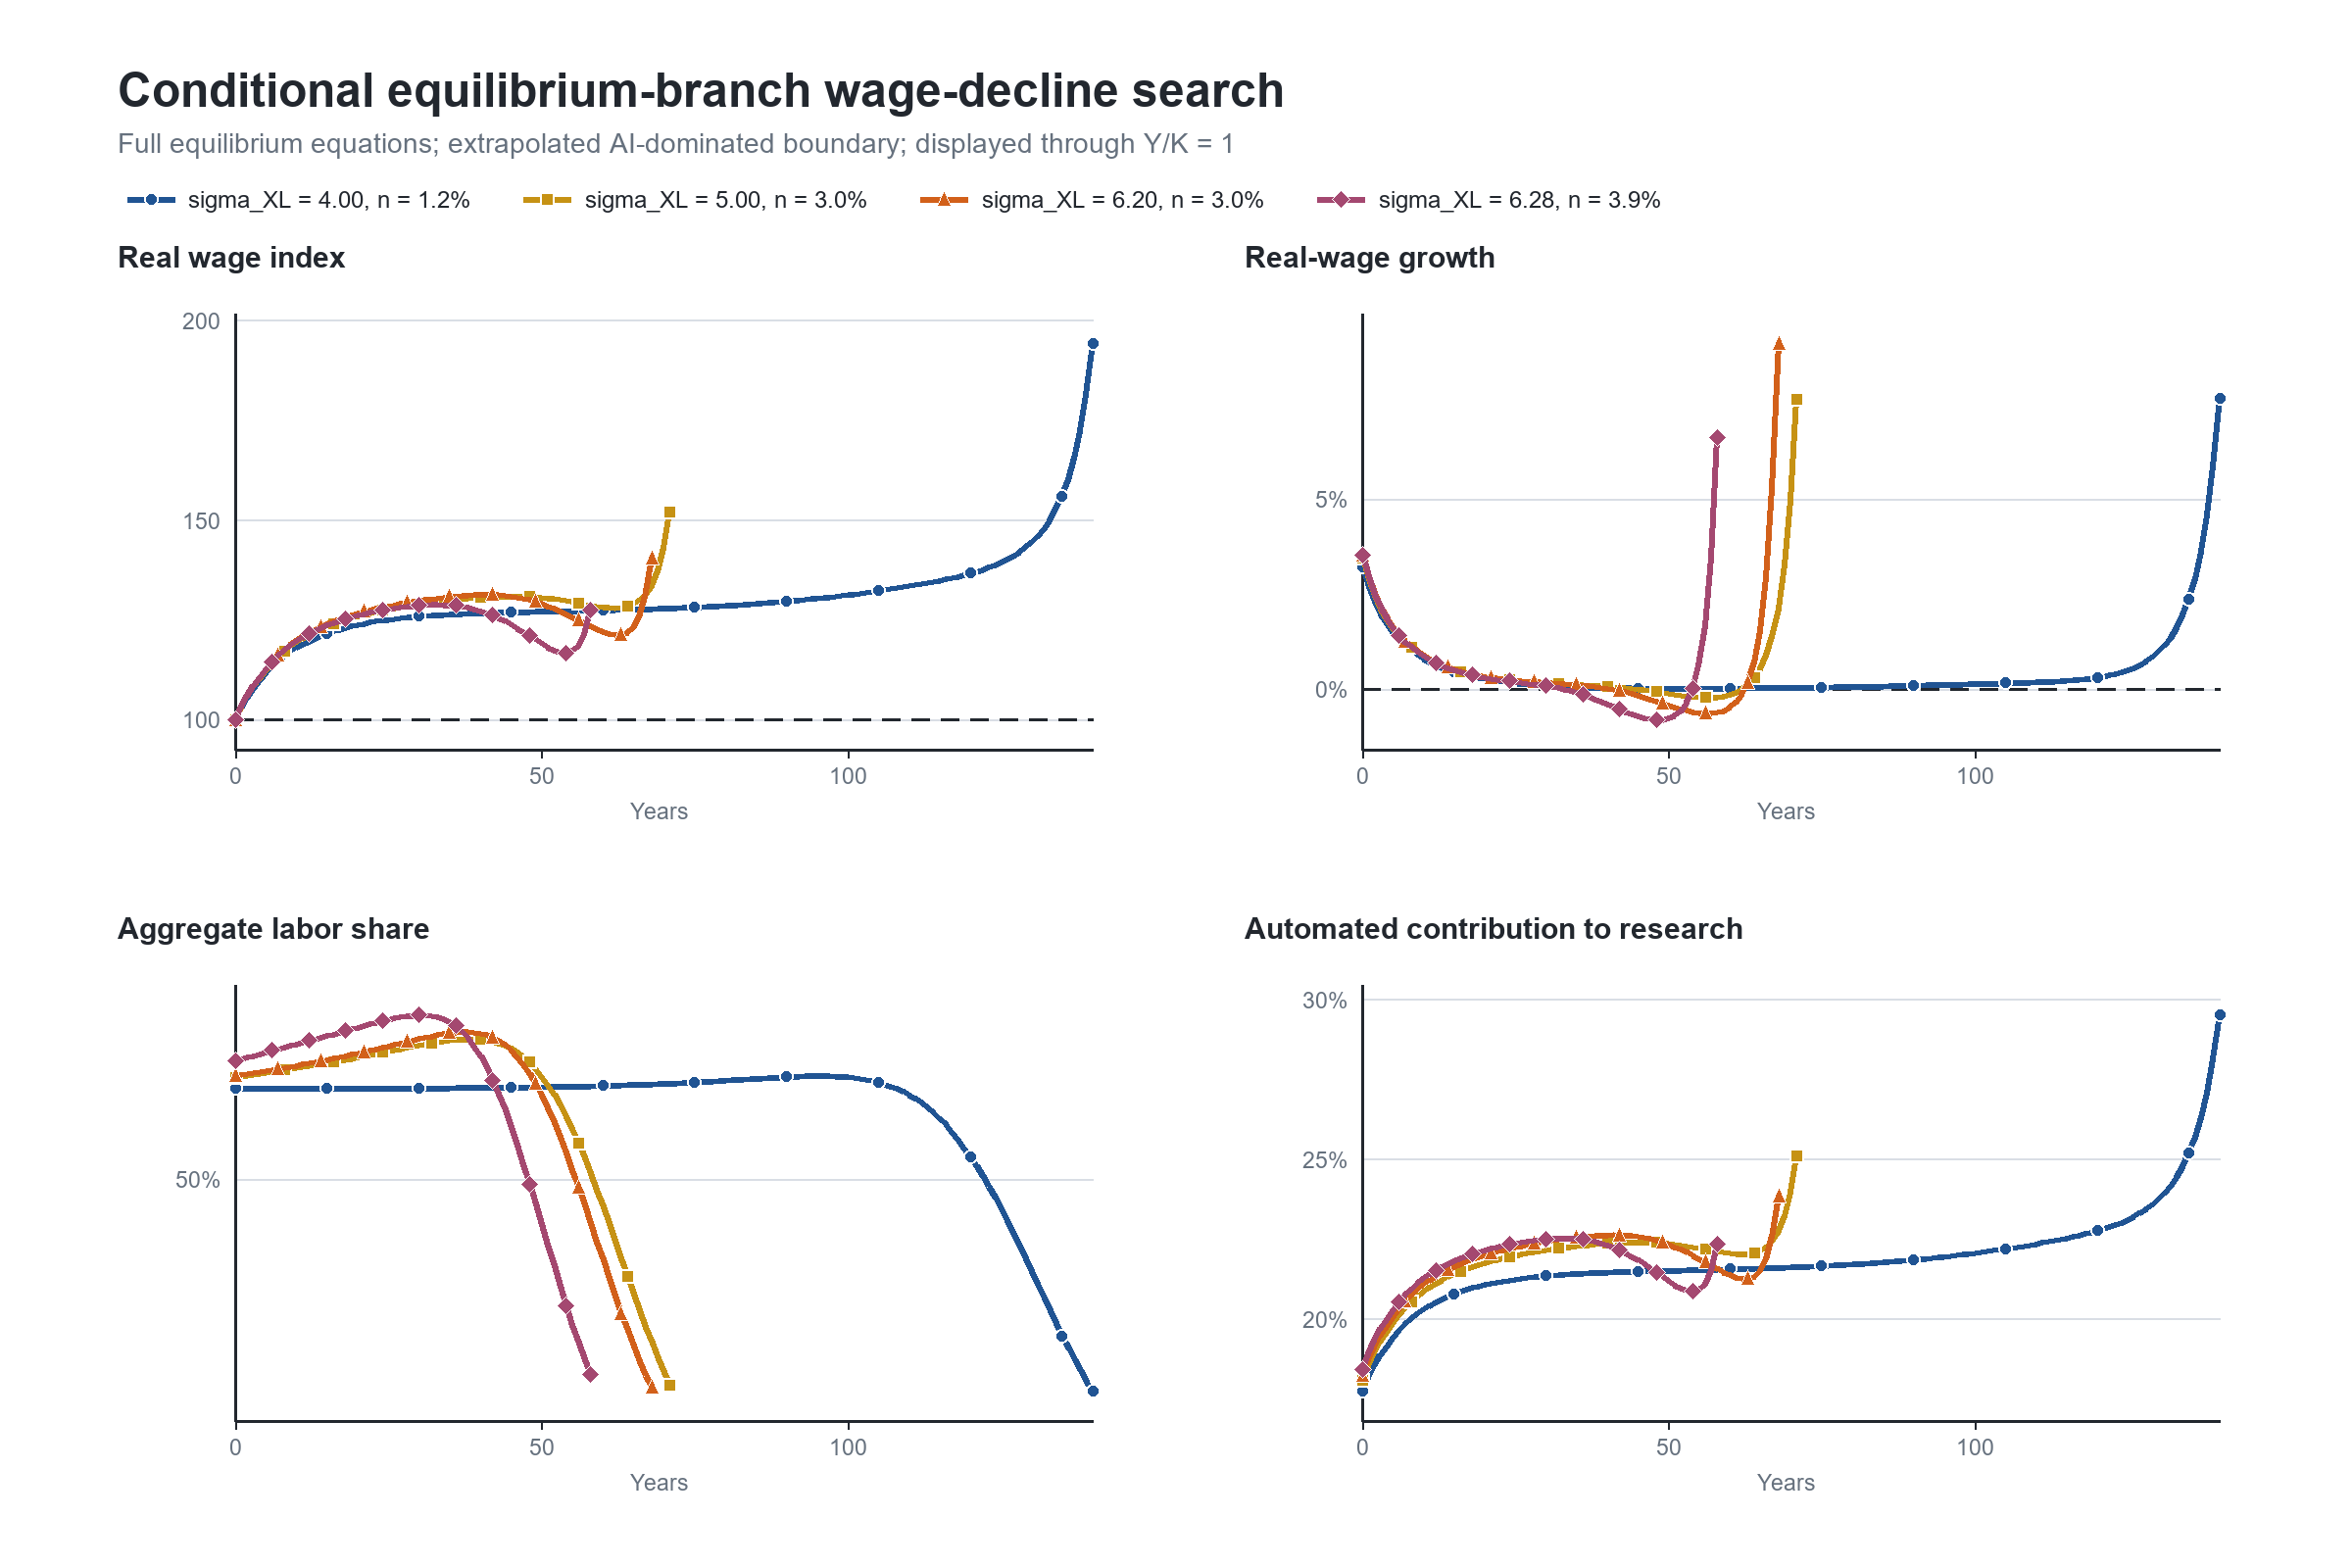
\includegraphics[width=\textwidth]{figures/equilibrium_wage_decline_search.png}
    \caption{Conditional equilibrium-branch search for wage declines. The wage
    index equals 100 at date zero. Growth rates and shares are percentages. The
    displayed transition ends when $Y/K$ reaches one so that the temporary wage
    decline remains visible. The aggregate labor share includes human researchers.}
    \label{fig:equilibrium-wage-decline-search}
\end{figure}

Proposition~\ref{prop:automated-research-wage} supplies an analytical sufficient
condition for eventual recovery: automated research per capita must diverge. The
conditional singular branch in result~\ref{cond:high-sigma-singular-scaling}
satisfies this condition in the parameter region covered by that result. The
wage-decline searches use still higher production elasticities and an extrapolated
terminal boundary, so their recovery remains numerical evidence rather than an
unconditional theorem for every admissible equilibrium. In these paths, the human
research share of population approaches one over the computed transition and
production labor becomes scarce. Moving the terminal value of $Y/K$ from 3 to 10
when $\sigma_{XL}=6.2$ changes the largest pre-year-60 difference in log wages by
0.0015. Moving it from 10 to 50 when $\sigma_{XL}=6.28$ changes the largest
pre-year-55 difference by 0.0010. The peak-to-trough decline in the last case moves
from 9.43 to 9.39 percent. The maximum equation residual across the four paths is
below $1.5\times10^{-5}$, and the resource constraint holds to machine precision.
These checks make the temporary decline and subsequent recovery robust within the
selected conditional branch. Establishing the result for every accelerating
equilibrium would additionally require proving that such an equilibrium necessarily
has $M/N\to\infty$, or another condition that implies wage divergence.

\subsection{Cross-case synthesis and limits of the evidence}

The audit changes the evidentiary status of several claims, even where it does not
change their mathematical content.
\begin{enumerate}[label=(\roman*)]
    \item Propositions~\ref{prop:wage-share-thresholds},
    \ref{prop:dynamic-labor-share}, and
    \ref{prop:research-employment-scale} are exact comparative-static or dynamic
    identities. The six paths satisfy them. Conditional
    result~\ref{cond:gradual-automation} describes what follows from a given
    relative-cost path rather than determining that path. The simulations also
    illustrate that a rising wage
    can coexist with a falling labor share and that declining human research
    intensity need not imply declining human research employment. The conditional
    searches above $1/\alpha$ add a distinct possibility: the wage can fall for a
    sustained interval and later recover while the labor share continues to decline.
    \item The Case I path with $\sigma_{XL}<1$ is consistent with the necessary limiting rates
    in conditional result~\ref{cond:nonunit-ces-steady-states}; the separate horizon test
    shows that its initial jump variables are stable. This is numerical support for
    the characterized limit, not a proof that the limit exists for every initial
    condition.
    \item The Case II path with $\sigma_{XL}=\sigma_{HM}=1$ approaches the fully Cobb--Douglas
    rates in \eqref{eq:full-cd-ga}--\eqref{eq:fully-cd-growth-rates}. Its automated
    research contribution remains $\omega_M$, while $H/N$ converges to a positive
    constant and $H/M$ converges to zero. This is an audited equilibrium example of
    human essentiality, not only a fixed-share mechanism calculation.
    \item The Case III path with $\sigma_{XL}=1$ and $\sigma_{HM}=2$ approaches the
    rates in conditional result~\ref{cond:ai-dominated-cd-limit} and is likewise
    stable when the terminal horizon is extended. It supports the conditional
    Cobb--Douglas characterization but does not convert its necessary conditions
    into a general existence theorem.
    \item In Case IV, the $\sigma_{XL}>1$ paths remain interior over their computed domains
    and are consistent with the lower-bound mechanism in the proof of
    Proposition~\ref{prop:gross-substitution-no-steady-state}: $Y/K$, the return, and
    consumption growth rise with capability. In conditional
    result~\ref{cond:high-sigma-singular-scaling}, however, $C/Y$
    and $qA/K$ are terminal boundary conditions. Only the convergence of the
    non-imposed ratios and the stability of the initial jumps and estimated boundary
    date constitute independent numerical evidence for the conditional singular
    branch.
    \item Conditional result~\ref{cond:singularity-conditions} concerns a reduced
    proportional-allocation closure, while
    conditional results~\ref{cond:sigma-hm-one-high-sigma-xl} and
    \ref{cond:knowledge-wedge} concern counterfactual research technology or a
    postulated shadow-value comparison. The six equilibrium computations do not
    test those results. Because $D_{\mathrm{CD}}$ and $D_{\mathrm{AI}}$ are positive
    under the common parameters, they also do not illustrate the zero- or
    negative-denominator branches. The Case III strong-feedback row in
    Table~\ref{tab:targeted-configurations} identifies a parameter region to be
    solved in future work; it is not plotted as an equilibrium path here.
\end{enumerate}

Finally, the residual audit verifies the canonical necessary conditions, not the
developer's global dynamic optimum in
\eqref{eq:developer-market-value-program}. Because the baseline parameters do not
guarantee global concavity, the numerical objects should be interpreted as locally
regular equilibrium branches selected by the stated endpoint conditions. Certifying
global optimality, existence, and uniqueness remains a separate task.

The previous proportional-allocation simulations remain useful for debugging and
for isolating mechanisms, but they cannot establish equilibrium claims. The new
paths change several quantitative conclusions. Most importantly, the optimizing
developer does not maintain a fixed research-spending share under complementarity,
and the household adjusts saving so that the return to capital and consumption
growth satisfy the Euler equation at every date. The wage-decline searches meet
those finite-domain equilibrium conditions, but their extrapolative terminal
condition leaves global branch selection unresolved.

\section{Extended model}
\label{sec:extended}

The extended model retains population growth, the integrated AI monopolist, the
nested production structure, the CES research aggregator, and the ideas production
function from Section~\ref{sec:toy}. It also retains
Assumption~\ref{ass:stable-human-essential-benchmark}. The model adds household
heterogeneity and richer accumulation of physical and computational capital. Regulated access to AI services
is treated as a policy counterfactual, not as a separate baseline industry.

\subsection{Households}

Each household type belongs to a population that grows at the common rate $n$.
Workers, researchers, and shareholders choose consumption and saving and own
specified shares of physical capital and firm equity. Workers receive production
wages, researchers receive research wages, and shareholders receive the integrated
developer's net profits.

This heterogeneity separates aggregate welfare from its distribution. Monopoly rents
can raise shareholder consumption while a high production elasticity $\sigma_{XL}$
between labor and AI services reduces labor income. The model will report aggregate
consumption, per-capita consumption, factor-income shares, and welfare by household type.

\subsection{Final-good firms}

Competitive final-good firms retain the production structure
\eqref{eq:final-production}--\eqref{eq:service-composite}. The substitution elasticity
$\sigma_{XL}$ determines how strongly firms replace production labor with AI services when
their relative price falls. Physical capital remains Cobb--Douglas with the CES
service composite. Final-good firms rent capital, hire production labor, and purchase
AI services at market prices.

\subsection{Integrated AI monopolist}

The integrated developer uses frontier capability $A_t$ and inference compute $U_t$
to supply quality-adjusted services $X_t$. It recognizes the demand generated by
final-good firms and chooses its price or quantity accordingly. Its operating rents
are the private return that links current market power to frontier research.

The baseline retains the normalization $X_t=A_tU_t$. A robustness exercise will allow
capability to affect inference efficiency through a separate mapping $B(A_t)$. This
will test whether the quantitative results depend on assigning the same state
variable to broad capability and services produced per unit of inference compute.

Inference and research compute are distinguished by use. The extended model can make
their resource cost depend on a common stock of computational capital and electricity,
without imposing an arbitrary fixed cap. This creates an endogenous opportunity cost
between current deployment and frontier research.

\subsection{Frontier research}

The integrated developer chooses human researchers and research compute,
\[
    \{H_t,M_t\},
\]
to maximize its market value. Capability evolves according to
\eqref{eq:ideas}--\eqref{eq:effective-research}. Human and automated-research
services are used simultaneously. Their equilibrium shares depend on the wage, the
common resource cost, and the substitution elasticity $\sigma_{HM}$. The private value of
an additional unit of capability reflects future cost reductions in supplying AI
services and the operating rents generated by those reductions.

\subsection{Government and social planner}

The government can regulate the access price for AI services, subsidize research
inputs, or pay an innovation prize. Net revenues are returned to households through
lump-sum transfers. The social planner values the current productive surplus from AI
services and the future knowledge benefits of capability. Its shadow value $Q_t$ can
therefore exceed the developer's private value $q_t$.

The planner's allocation provides the welfare benchmark. Comparing its conditions
with those of the monopolist identifies separately the static service-market markup
and the dynamic knowledge and appropriability wedge. The policy instruments are
specified in Section~\ref{sec:regulation}.

\subsection{Equilibrium}

Given a policy rule, an equilibrium consists of paths for population, consumption and
saving by household type, physical and computational capital, investment, production
and research labor, AI services, inference and research compute, and frontier
capability. Prices include the return to capital, wages, the price of AI services, the
common price of standardized compute when its supply is endogenous, and the private
shadow value of capability.

Households optimize given prices, profits, taxes, and transfers. Final-good firms
maximize profits. The integrated developer chooses current AI supply and frontier
research to maximize its market value subject to the ideas production function and
the policy regime. Labor and goods markets clear, and the laws of motion for
population, capital, compute capacity, and capability hold.

\subsection{Solution}

The solution traces a continuous change in the research-input composition. The
automated share is solved jointly with wages, investment, automated-research
services, and the private value of capability. Population growth anchors the
human-dominated benchmark. In the AI-dominated limit, capability growth depends on
the growth of automated-research services and on $\phi$ and $\eta$.
The solution must keep the two acceleration channels separate. It will report the
path of the research-feedback denominator as the automated contribution changes and
will distinguish that path from the production-side effect of $\sigma_{XL}>1$ on
the output--capital ratio and the return to capital.

For each policy regime, the model solves household and firm optimality conditions
together with market clearing and the state equations. The laissez-faire monopoly
and the regulated allocations are computed from the same initial conditions and
technological parameters. The social-planner allocation then decomposes the welfare
gap into restricted current deployment, imperfect appropriation of innovation
benefits, and distributional effects.

The quantitative solution will report both the production-labor share,
$w_tL_t/Y_t$, and the aggregate labor-income share, $w_tN_t/Y_t$. The first
isolates substitution between production labor and AI services. The second also
incorporates the endogenous allocation of labor to frontier research. This
distinction is necessary for taking Proposition
\ref{prop:wage-share-thresholds} from a conditional production result to a
general-equilibrium distributional result.

\subsubsection{Quantitative objects}

The solution requires:
\begin{enumerate}[label=(\roman*)]
    \item population growth $n$ and the allocation of labor between production and
    research;
    \item the substitution elasticity $\sigma_{XL}$ between production labor and AI
    services, together with the CES weights $(\omega_L,\omega_X)$;
    \item the common unit resource cost $\xi$ of inference and research compute and,
    in the richer version, the law of motion for computational capital;
    \item the research-substitution elasticity $\sigma_{HM}$ and the CES weights
    $(\omega_H,\omega_M)$;
    \item the elasticities $\phi$ and $\eta$ in the ideas production function;
    \item a capability-dependent mapping $\lambda(A)$ for automated research in a
    robustness extension;
    \item the mapping $B(A)$ from capability to inference efficiency in the
    robustness exercise; and
    \item the degree to which operating rents and innovation prizes let the
    developer appropriate the social value of capability.
\end{enumerate}
These objects determine human-dominated growth, the speed of research automation,
whether recursive feedback is compatible with constant growth, whether production
admits a finite-growth limit, the output cost of monopoly pricing, and the gap
between private and social research.

\section{Extension: research tasks and fixed automation costs}
\label{sec:task-extension}

The baseline CES treats human and automated research as two continuously variable
inputs with a constant elasticity of substitution. This is useful for characterizing
prices, shares, and balanced growth, but it suppresses an extensive margin: an AI
system may be able to perform some research tasks and not others. It also suppresses
the engineering cost required to make a task reliably automatable. This section
introduces those margins as an extension rather than changing the baseline model.
The parameter values continue to satisfy
Assumption~\ref{ass:stable-human-essential-benchmark} when the task technology is
compared with the human-essential Cobb--Douglas benchmark.
The formulation connects the paper to task-based models of automation and research
\citep{aghionjonesjones2019,acemoglu2025,jones2025rd}.

\subsection{Research tasks}

Frontier research requires a continuum of tasks indexed by $i\in[0,1]$. Let
$e_t(i)$ denote the quantity of task $i$ completed at date $t$. Effective research
is a CES aggregate across tasks,
\begin{equation}
    E_t
    =
    \left[
        \int_0^1 e_t(i)^{(\zeta-1)/\zeta}\dd i
    \right]^{\zeta/(\zeta-1)},
    \label{eq:task-research-aggregator}
\end{equation}
where $\zeta$ measures substitution across research tasks. A low $\zeta$ captures
the idea that progress can be constrained by a small set of bottleneck tasks. The
ideas production function remains
\begin{equation}
    \dot A_t=\chi A_t^\phi E_t^\eta.
    \label{eq:task-ideas-production}
\end{equation}

Humans produce task $i$ according to
\begin{equation}
    e^H_t(i)=a_H(i)h_t(i),
    \qquad
    c^H_t(i)=\frac{w_t}{a_H(i)},
    \label{eq:human-task-cost}
\end{equation}
where $c^H_t(i)$ is the human variable cost of one unit of the task. If task $i$
has been automated, research compute produces
\begin{equation}
    e^M_t(i)=a_M(i,A_t)m_t(i),
    \qquad
    c^M_t(i,A_t)=\frac{\xi_t}{a_M(i,A_t)}.
    \label{eq:machine-task-cost}
\end{equation}
Capability can increase $a_M(i,A)$, but the function is allowed to differ across
tasks. A task that the current frontier cannot perform has $a_M(i,A_t)=0$.

\subsection{Fixed costs and the automation decision}

Using AI for task $i$ requires an annuitized fixed cost $F_i(A_t)$. This cost covers
the task-specific engineering needed to construct evaluations, adapt workflows,
integrate tools, and verify reliability. For a required quantity $q_t(i)$, the two
cost schedules are
\begin{align}
    C^H_t(i,q)&=c^H_t(i)q,
    \label{eq:human-task-total-cost}\\
    C^M_t(i,q)&=F_i(A_t)+c^M_t(i,A_t)q.
    \label{eq:machine-task-total-cost}
\end{align}
The developer automates the task if
\begin{equation}
    q_t(i)\left[c^H_t(i)-c^M_t(i,A_t)\right]
    \geq F_i(A_t),
    \label{eq:task-automation-condition}
\end{equation}
provided $c^M_t(i,A_t)<c^H_t(i)$. Equivalently, the scale threshold is
\begin{equation}
    q^*_t(i)
    =
    \frac{F_i(A_t)}
    {c^H_t(i)-c^M_t(i,A_t)}.
    \label{eq:task-scale-threshold}
\end{equation}
An AI system can therefore have a lower marginal cost for a task without being used
at small scale. The fixed cost must first be amortized over enough task output. If
$F_i$ is a sunk rather than an annuitized cost, condition
\eqref{eq:task-automation-condition} compares the fixed cost with the discounted
stream of expected variable-cost savings; the economic threshold is unchanged.

Define the set of tasks automated at date $t$ as
\begin{equation}
    \mathcal A_t
    \equiv
    \left\{
        i\in[0,1]:
        c^M_t(i,A_t)<c^H_t(i),\quad
        q_t(i)\geq q^*_t(i)
    \right\},
    \qquad
    a_t\equiv\int_0^1\mathrm{I}\{i\in\mathcal A_t\}\dd i.
    \label{eq:automated-task-set}
\end{equation}
Here $\mathrm{I}\{\cdot\}$ is the indicator function. The measure $a_t$ is an
endogenous automation frontier. It expands when capability
raises task-level AI productivity, when the research wage rises relative to compute
cost, when capability lowers fixed integration costs, or when the scale of research
increases enough to amortize those costs.

\subsection{Relation to the CES benchmark}

The task model separates two margins that the baseline CES compresses into the
single share $s^M_t$. The intensive margin changes the human--machine mix within
tasks that both inputs can perform. The extensive margin changes the set
$\mathcal A_t$. When task technologies and costs have a smooth distribution, the
aggregate response of machine expenditure to $w_t/\xi_t$ can resemble the CES law
in \eqref{eq:automation-odds} over a range of the state space. The implied aggregate
elasticity need not, however, be constant: it depends on the density of tasks close
to the threshold in \eqref{eq:task-automation-condition}.

Fixed costs also explain why the initial automated share can be close to zero even
if some AI systems are technically capable of assisting research. At low research
scale, few tasks generate savings large enough to cover $F_i(A_t)$. As research
expands, more tasks cross their scale threshold. This mechanism complements the
baseline relative-price condition in
\eqref{eq:initial-human-dominance-condition}; it does not replace it.

If every task remains essential and $a_t<1$, the unautomated set can continue to
constrain effective research even when automated tasks become arbitrarily cheap.
If $a_t\to1$, the human bottleneck disappears. The asymptotic growth condition then
approaches the AI-dominated denominator $D_{\mathrm{AI}}$. If $a_t$ converges to an
interior value, the relevant feedback remains weaker and can preserve balanced
growth. Task heterogeneity therefore provides a microeconomic interpretation of
the transition between the human-dominated and AI-dominated regimes.

\subsection{Scale feedback, market structure, and equilibrium}

The fixed-cost formulation creates a scale feedback absent from the constant-
elasticity benchmark. A larger research program raises $q_t(i)$, which makes more
tasks worth automating. Automation lowers the unit cost of effective research and
can induce a further expansion of the research program. If many tasks have similar
thresholds, this feedback can produce a rapid transition or multiple local
equilibria. Whether it does is a quantitative property of the distribution of
$F_i$, $a_H(i)$, and $a_M(i,A)$; it does not follow from fixed costs alone.

The integrated monopolist may also have a private scale advantage. A task-specific
automation investment can be reused across model generations or commercial uses,
allowing the developer to spread $F_i$ over a larger base. Knowledge spillovers
create the opposite wedge: if other firms can reuse the resulting evaluations,
tools, or methods, the private developer does not capture the full return to paying
the fixed cost. The planner and the monopolist can consequently choose different
automation frontiers even at the same $A_t$ and $w_t/\xi_t$.

An equilibrium in this extension consists of the objects in Section
\ref{sec:extended}, task quantities $q_t(i)$, human and automated task inputs,
and the set $\mathcal A_t$. Conditional on aggregate states and prices, the
developer first compares the two cost schedules for every task. It then chooses the
task quantities that minimize the cost of producing $E_t$ and chooses the scale of
research using the private shadow value of capability. Market clearing and the
state equations determine the aggregate transition. A quantitative version must
calibrate the distribution of task-level fixed costs and AI productivities; the CES
model remains the parsimonious baseline until those objects can be disciplined.

\section{Market-regulation scenarios}
\label{sec:regulation}

The regulatory analysis compares policies under the same technology, initial
conditions, and population path. The central issue is that the current-deployment
distortion and the research-incentive distortion operate through different margins.

\subsection{Laissez-faire monopoly}

The integrated developer chooses the quantity and price of AI services together with
human and computational research inputs. It receives all operating rents and no
additional research support. This scenario provides the benchmark paths for AI
deployment, capability, research, monopoly rents, per-capita consumption, and the
automated share of research.

\subsection{Regulated access price}

A price cap or access rule moves the AI-service price toward marginal cost. It expands
current use of AI at a given capability but reduces operating rents and therefore the
private shadow value of frontier capability. The experiment measures the static gain
from deployment against the induced change in research and its input composition.

\subsection{Research subsidy or innovation prize}

If an explicit planner problem implies $Q_t>q_t$, a subsidy to human research or
research compute, or an innovation prize contingent on capability improvements, can
target the resulting wedge $(Q_t-q_t)F_{M,t}$. The baseline model does not establish
the sign of this wedge. The distinction matters for implementation: an input subsidy
rewards expenditure, while a prize rewards measured output. Either instrument can
increase private research without requiring a high markup on all current uses of AI.

\subsection{Joint price and research policy}

A joint policy combines regulated access to current AI services with explicit
remuneration for frontier innovation. In principle, the access rule targets the
static monopoly distortion. A research instrument would address a separate dynamic
wedge only if a fully specified planner problem establishes one. A quantitative
welfare extension would determine whether one instrument is enough or whether this
two-instrument policy is required.

\subsection{Policy comparison}

For each regime, the model will report:
\begin{enumerate}[label=(\roman*)]
    \item the path of the automated share of effective research;
    \item the paths of AI capability, aggregate output, and output per capita;
    \item consumption and factor-income shares;
    \item AI-service prices, quantities, markups, and developer rents;
    \item the level and composition of research; and
    \item aggregate welfare and welfare by household type.
\end{enumerate}
The comparison will distinguish policies that change current deployment from those
that change the private appropriation of innovation benefits. It will also show how
population growth affects the human-dominated benchmark against which an
automation-driven change in the growth regime is measured.

\section{Conclusion}
\label{sec:conclusion}

The economic consequences of advanced AI depend on more than whether machines can
perform existing jobs. A distinct transition occurs when AI can perform the research
required to produce better AI. The toy model represents this transition as a gradual
change in the composition of research. When human and automated-research services are
gross substitutes ($\sigma_{HM}>1$), the automated share rises with the research wage
relative to its unit resource cost.

Population growth matters while human research dominates. With $\phi<1$ and a
constant research-employment share, capability growth is semi-endogenous and equals
$\eta n/(1-\phi)$. Research automation creates a separate feedback from capability
to output, from output to automated research, and from research back to capability.
The fully Cobb--Douglas counterfactual isolates this channel. Its reduced dynamics
are stable when
$D_{\mathrm{CD}}=1-\phi-\eta\omega_M\omega_X/\omega_L>0$.
At $D_{\mathrm{CD}}=0$, capability is double exponential but remains finite at every
finite date. At $D_{\mathrm{CD}}<0$, the reduced system reaches a finite-time
singularity. Hence explosive growth does not require $\sigma_{XL}>1$.

When $\sigma_{HM}>1$, the automated contribution to research changes endogenously.
The relevant denominator becomes
$D(s^M_t)=1-\phi-\eta\upsilon s^M_t$ and declines as automated research gains weight.
Its AI-dominated limit,
$D_{\mathrm{AI}}=1-\phi-\eta\upsilon$, must be positive for the stated finite
constant-growth candidate. This condition is stricter than the human-essential one because the
entire growth of automated research, rather than only the Cobb--Douglas weight
$\omega_M$, feeds back into capability. A temporary negative value is not sufficient
for a singularity; the negative-denominator episode must be sufficiently persistent
to satisfy the integral condition derived in the paper.

These feedback results have a deliberately limited status. The baseline parameters
keep $D_{\mathrm{CD}}$ and its AI-dominated counterpart positive. The zero- and
negative-denominator cases are analytical counterfactuals under proportional
allocation. They do not establish that the fully optimizing monopoly follows the
same path: consumption, research, or another allocation can reach a boundary first.
Likewise, a failed constant-growth condition is not by itself proof of a finite-time
singularity.

The task-based extension identifies a separate extensive margin. Even when AI has a
lower marginal cost for a research task, a fixed integration and verification cost
can make human performance cheaper at low scale. Capability growth, a higher research
wage, or an expansion of the research program can move tasks across their automation
thresholds. The resulting aggregate elasticity can vary endogenously with the
distribution of task-level costs, while the CES remains the parsimonious baseline.

The production elasticity $\sigma_{XL}$ also separates the wage response from the
response of the production-labor share. An expansion of AI services reduces this share when
$\sigma_{XL}>1$, but it raises the wage when $\sigma_{XL}<1/\alpha$. Hence both outcomes occur
when $1<\sigma_{XL}<1/\alpha$. This static result is a benchmark, not the paper's
standalone contribution. In general equilibrium, capital deepening and the
reallocation of workers between production and research also affect wages and the
aggregate labor share. More precisely, aggregate labor-share growth equals
production labor-share growth plus the growth of population relative to production
labor. A rising human-research employment share raises the aggregate share relative
to the production share; a declining human-research share lowers it.

The capital-deepening benchmark clarifies which part of the growth result is specific
to recursive AI research. If the labor substitute is an ordinary reproducible capital
service, gross substitution can drive labor's share to zero while the wage rises, but
constant saving produces at most an asymptotically linear $AK$ technology with a
constant growth rate. In the baseline model, capability also lowers the unit resource
cost of AI services and is produced with AI research. This additional loop can make
the output--capital ratio and the return to capital increase without bound. The
common ingredient in the paper's acceleration mechanisms is therefore recursive
improvement, not gross substitution or capital deepening alone. A nonpositive
research-feedback denominator can generate acceleration at unit elasticities;
$\sigma_{XL}>1$ provides a distinct production-side amplifier when capability is
unbounded.

Research automation also has two distinct margins within the AI-development
industry. The ratio $H/M$ measures human intensity, while $H/N$ measures the scale
of human research employment. The first can fall while the second rises. This occurs
when automated research per capita expands more rapidly than human input per unit of
automated research contracts. In the equilibrium complementarity path, $H/N$
declines monotonically. In the Cobb--Douglas equilibrium, it rises during the first
part of the transition and later converges to zero while the automated research
share approaches one. The asymptotic disappearance of human research as a relative
input therefore does not imply that human research employment must fall throughout
the transition.

The production elasticity supplies the second dimension of the growth classification.
When $\sigma_{XL}<1$, the low-elasticity candidate leaves labor essential
and makes the productive return to further reductions in the unit cost of AI services
vanish. At $\sigma_{XL}=1$, positive wage growth would make automated research
asymptotically dominant. When $\sigma_{XL}>1$ and the effective unit cost of AI
services vanishes relative to capital intensity, the production-labor share converges
to zero. The unconditional nonexistence result is narrower and stronger where it
applies: no interior steady state can combine finite constant growth rates with a
positive constant capability-growth rate. The qualification is important:
$\sigma_{XL}>1$ alone does not exclude a boundary path with bounded capability.

The discontinuity at unit elasticity is an infinite-horizon classification, not a
jump in finite allocations. At every finite relative price, the CES contribution
share is continuous in $\sigma_{XL}$. But the limits $w/p^X\to\infty$ and
$\sigma_{XL}\downarrow1$ do not commute: the share remains $\omega_X$ at exactly
one and converges to one for every fixed elasticity above one. Under the paper's
high-capability regularity condition, unbounded capability induces this relative-price
limit. The relative-price threshold for the
transition diverges as $\sigma_{XL}$ approaches one. This makes the result a singular
perturbation and explains why an economy with $\sigma_{XL}$ only slightly above one
can look Cobb--Douglas over an extremely large range of finite relative prices
without possessing a finite-growth steady state asymptotically.

The numerical experiments solve the decentralized perfect-foresight canonical system.
Investment and research spending are endogenous, the household Euler equation holds,
and the developer satisfies its research first-order and costate conditions. With
$\sigma_{XL}=0.75$, output per capita falls initially, recovers, and then approaches
a constant level even though capability continues to grow. By year 600,
output-per-capita growth is 0.0056 percent and capability growth is 0.703 percent,
close to its analytical limit of 0.675 percent. The production-labor share rises as
labor becomes the bottleneck. With $\sigma_{XL}=1$ and $\sigma_{HM}=2$, capability
growth rises gradually and reaches 2.271 percent by year 2,000. Output- and
consumption-per-capita growth then approach 0.568 percent, while the automated
research share approaches one. Changing only the research elasticity to
$\sigma_{HM}=1$ lowers the limiting capability-growth rate to 1.738 percent and
per-capita output growth to 0.435 percent. The automated research contribution then
remains at 35 percent and human research employment converges to a positive share
of the population, even though $H/M$ converges to zero.
These transitions confirm that the asymptotic regime need not be a good medium-run
approximation.

For $\sigma_{XL}>1$, the paper solves a free-boundary equilibrium branch instead of
imposing a finite-growth terminal state. Conditional on an AI-dominated singular
limit, $g_A/(Y/K)$, the consumption share, the research-resource share, and $qA/K$
converge to constants, while $Y/K$ grows in inverse proportion to the remaining
time. The terminal conditions impose the limiting values of $C/Y$ and $qA/K$;
those two ratios are not independent validation moments. For $\sigma_{XL}=1.35$,
1.50, and 2.00, the non-imposed growth and resource-share ratios approach their
analytical predictions, while the initial jumps and estimated boundary dates remain
stable as the boundary moves outward. The estimated dates are 333.38, 280.45, and 209.08
years, respectively. These dates illustrate the comparative dynamics of the model;
they are not calibrated forecasts.

The return to capital supplies the price counterpart to these quantity dynamics.
Because saving is endogenous, the net return is an intertemporal equilibrium price
rather than a marginal product evaluated along an imposed investment path. It
converges to 4 percent under complementarity and to 4.568 percent in the
Cobb--Douglas AI-dominated limit. Under gross substitution, the net return first
remains moderate and then diverges with $Y/K$. Output and consumption growth also
accelerate. The real wage rises in all three reported gross-substitution paths,
while the aggregate labor share approaches zero. The earlier fixed-share paths
remain available as mechanism exercises but are not evidence about equilibrium
takeoff, interest rates, or wage declines.

A separate conditional search considers production elasticities above the static
wage threshold $1/\alpha$ and population growth as high as 3.9 percent. These paths
satisfy the canonical equilibrium equations on their computed domains but
extrapolate the AI-dominated terminal boundary beyond the region established by the
analytical result. Wage growth becomes negative in three of the four selected
configurations. The largest peak-to-trough wage decline is 9.39 percent when
$\sigma_{XL}=6.28$ and $n=3.9$ percent. The wage subsequently recovers and its trough
remains 16.72 percent above the initial wage. Capital deepening contributes to the
recovery, while the expansion of human employment in AI research makes production
labor scarce. More generally, the research first-order conditions imply that the
wage diverges whenever automated research per capita diverges. They also imply that,
with diminishing returns to the capability stock, a finite-time capability
singularity cannot occur while the wage remains bounded. The conditional singular
branch satisfies the stronger per-capita condition, so any finite wage decline on
that branch must eventually be reversed in levels. The high-elasticity wage-decline
searches use an extrapolated terminal boundary; proving recovery for every
infinite-horizon accelerating equilibrium still requires showing that acceleration
necessarily makes automated research per capita diverge.

Taken together, these results explain why the automation of AI research matters for
humans whether the real wage rises or falls temporarily. It can change the growth regime, reduce
labor's share of an expanding economy, increase the return to capital, and shift
income toward the owners of AI firms and other productive assets. It can also reduce
the number of humans required per unit of research without reducing human research
employment, because the development industry may expand faster than its human
intensity falls. The distinction between finite and asymptotic behavior is equally
important: observed stability over a finite range of capability and relative prices
does not by itself identify the long-run regime.

The current model does not establish whether an acceleration regime improves human
welfare. Monopoly rents accrue to a representative household, so the model abstracts
from unequal ownership and understates the distributional importance of a declining
labor share. It also excludes agency failures, misalignment, existential damage, and
political power. The numerical paths reported in the paper solve the decentralized
canonical equilibrium conditions. For $\sigma_{XL}>1$, they use the conditional singular
ratios derived in conditional result~\ref{cond:high-sigma-singular-scaling} and pass a
free-boundary convergence test. This procedure provides numerical evidence for a
locally regular singular branch from the stated initial conditions, but it is not a
proof of the developer's global dynamic optimality, global existence, or uniqueness.
The paper's acceleration and singularity calculations
remain conditional on the assumptions stated in the relevant conditional results and are
not quantitative forecasts. The paper does not assign probabilities to those
regimes or determine their full welfare ranking.

Market power creates a genuine policy trade-off. The monopolist restricts the current
supply of AI services, but its operating rents raise the private return to frontier
research. An explicit planner extension may value capability more than the monopolist
does; if it establishes $Q_t>q_t$, private research is insufficient at the private
allocation. The current model does not derive that inequality. Regulating the
AI-service price without replacing the lost innovation return can therefore improve
current deployment while slowing capability growth. The natural policy comparison is
between laissez-faire monopoly, regulated access, explicit research support, and a
joint policy that targets both margins.

A further extension should make explicit an agency problem that is only implicit in
the current model. As $H/M$ falls and automated systems choose a larger share of the
experiments, code, and model modifications that move the frontier, human owners and
researchers may become less able to observe their actions, verify their objectives,
or anticipate the consequences of every research decision. Supervision would then
be a costly choice rather than an implicit component of $H_t$. More intensive
oversight could reduce the probability that automated research departs from the
human principal's objectives, but it could also slow capability growth. Research
automation would thus generate a principal--agent problem with costly monitoring in
the spirit of \citet{holmstrom1979}.

Market structure may alter this trade-off, although its sign is not predetermined.
A protected monopolist internalizes a larger share of the loss to its installed
rents and franchise value if its automated researchers escape effective control. It
also faces less pressure to preempt a competitor. These forces may induce it to
moderate capability growth or invest more in supervision. Under monopolistic
competition, by contrast, each developer captures the private benefit of arriving
first, while part of the expected cost of inadequate supervision is borne by rivals
and society. Firms may consequently underinvest in oversight in order to accelerate
development and preserve their competitive position. Monopoly is not, however, a
guarantee of better control: concentration creates its own governance problems, and
the threat of entry or a foreign rival can restore the race incentive. The race and
slowdown branches in \citet{kokotajlo2025} illustrate precisely this tension: even a
concentrated frontier developer that observes evidence of misalignment may hesitate
to pause when another developer is close behind. A formal extension should therefore
allow developers to choose innovation speed and supervisory effort, make the
probability of an agency failure depend on automation and oversight, and compare
monopoly with monopolistic competition. If human research provides supervision that
is socially valuable but not fully remunerated, the extension could also evaluate a
second-best policy that subsidizes $H_t$ and taxes $M_t$. The purpose of these wedges
would not be to preserve human research employment, but to correct the effect of the
research-input mix on agency risk. A subsidy to verifiable supervision or liability
for agency failures would generally target the distortion more directly. A subsidy
to $H_t$ and a tax on $M_t$ become relevant when supervision cannot be separately
observed or contracted. These policies cannot be evaluated in the current model,
which contains neither agency losses nor an explicit supervision technology. The
central open question is when the
monopolist's internalization of agency losses dominates the governance costs of
concentration, and when competition turns effective supervision into an externality.


\bibliographystyle{apalike}
\bibliography{references}

\appendix
\section{Proofs}
\label{sec:appendix-proofs}

\begin{proof}[Derivation for conditional result~\ref{cond:capital-deepening-benchmark}]
Let $\widetilde k_t\equiv\widetilde K_t/L_t$. Equations
\eqref{eq:capital-benchmark-production}--
\eqref{eq:capital-benchmark-allocation} give
\begin{equation}
    \frac{\widetilde Y_t}{\widetilde K_t}
    =
    \zeta^\alpha
    \left[
        \omega_L\widetilde k_t^{-\varrho_K}
        +\omega_K(1-\zeta)^{\varrho_K}
    \right]^{(1-\alpha)/\varrho_K}.
    \label{eq:proof-capital-benchmark-output-capital}
\end{equation}
When $\varrho_K>0$, this expression is strictly decreasing in
$\widetilde k_t$, diverges as $\widetilde k_t\downarrow0$, and converges to
$B_K(\zeta)$ as $\widetilde k_t\to\infty$. Capital accumulation implies
\begin{equation}
    \frac{\dot{\widetilde k}_t}{\widetilde k_t}
    =
    s_K\frac{\widetilde Y_t}{\widetilde K_t}
    -(\delta+n).
    \label{eq:proof-capital-benchmark-law}
\end{equation}
If $s_KB_K(\zeta)<\delta+n$, monotonicity and the two boundary limits imply
a unique finite stationary value of $\widetilde k_t$. If
$s_KB_K(\zeta)>\delta+n$, equation
\eqref{eq:proof-capital-benchmark-law} converges to the positive constant
$s_KB_K(\zeta)-\delta-n$. Hence
$g_{\widetilde K}=n+g_{\widetilde k}=s_KB_K(\zeta)-\delta$; asymptotic
linearity gives the same rate for output. At equality, the right-hand side is
positive at every finite $\widetilde k_t$ and converges to zero, so
$\widetilde k_t$ diverges while its growth rate vanishes.

The inner labor contribution satisfies
$1-s^{K_2}_t\sim c\widetilde k_t^{-\varrho_K}$ for a positive constant $c$.
Since $\widetilde Y_t/L_t\sim B_K(\zeta)\widetilde k_t$, the competitive
wage obeys
\[
    w_t
    =(1-\alpha)(1-s^{K_2}_t)\frac{\widetilde Y_t}{L_t}
    \sim \widetilde c\,
    \widetilde k_t^{1-\varrho_K}
    =\widetilde c\,
    \widetilde k_t^{1/\sigma_{KL}}
\]
for a positive constant $\widetilde c$. The labor share converges to zero and,
on the positive-growth branch,
$g_w=g_{\widetilde k}/\sigma_{KL}=g_{\widetilde Y/L}/\sigma_{KL}$.
\end{proof}

\begin{proof}[Proof of Proposition~\ref{prop:wage-share-thresholds}]
The CES expenditure share in \eqref{eq:ai-composite-share} implies
\[
    \frac{\partial\log(1-s^X_t)}{\partial\log X_t}
    =
    -\left(1-\frac{1}{\sigma_{XL}}\right)s^X_t.
\]
The output elasticity follows directly from
\eqref{eq:final-production}--\eqref{eq:service-composite}. Combining these two
expressions with \eqref{eq:labor-demand} yields
\eqref{eq:labor-share-ai-elasticity} and \eqref{eq:wage-ai-elasticity}.
\end{proof}

\begin{proof}[Proof of Proposition~\ref{prop:dynamic-labor-share}]
Log-differentiating \eqref{eq:production-labor-share} and using the CES share
equation gives \eqref{eq:dynamic-production-labor-share}. Since
$L_t=(1-h_t)N_t$, $g_{L,t}=n-\dot h_t/(1-h_t)$.
Log-differentiating \eqref{eq:aggregate-labor-share} then gives
\eqref{eq:dynamic-aggregate-labor-share}.
\end{proof}

\begin{proof}[Derivation for conditional result~\ref{cond:gradual-automation}]
Equation~\eqref{eq:automation-odds} gives
\[
    \frac{s^M_t}{1-s^M_t}
    =
    \left(\frac{\omega_M}{\omega_H}\right)^{\sigma_{HM}}
    \left(\frac{w_t}{\xi}\right)^{\sigma_{HM}-1}.
\]
If $\sigma_{HM}>1$ and $w_t/\xi\to\infty$, the right-hand side diverges and
$s^M_t\to1$. Moreover, the unit cost in
\eqref{eq:research-unit-cost} converges to
\[
    P^E_t\longrightarrow
    \omega_M^{-\sigma_{HM}/(\sigma_{HM}-1)}\xi.
\]
The first expression in \eqref{eq:research-conditional-demands} then implies
$H_t/E_t\to0$. If $w_t/\xi$ remains bounded, the odds in
\eqref{eq:automation-odds} remain bounded, so $\sigma_{HM}>1$ does not by itself imply
$s^M_t\to1$.
\end{proof}

\begin{proof}[Proof of Proposition~\ref{prop:research-employment-scale}]
Take growth rates in equation~\eqref{eq:research-input-ratio} to obtain the first
identity. Combine it with equation~\eqref{eq:human-research-scale-identity} and
$g_N=n$ to obtain the second. The two sign conditions follow directly.
\end{proof}

\begin{proof}[Proof of Proposition~\ref{prop:automated-research-wage}]
Taking the $1/\sigma_{HM}$ power of
\eqref{eq:research-input-ratio} and solving for the wage gives the equality in
\eqref{eq:wage-automated-research-lower-bound}. Labor feasibility implies
$0<H_t\leq N_t$, so $M_t/H_t\geq M_t/N_t$ and gives the inequality. Because
$\xi$, the CES weights, and $\sigma_{HM}$ are positive and constant,
$M_t/N_t\to\infty$ implies $w_t\to\infty$. Log differentiation of the equality
gives \eqref{eq:wage-research-scale-growth}.

For the finite-time claim, suppose instead that $w_t$ were bounded on a terminal
interval $[t_0,T^*)$. Equation~\eqref{eq:research-input-ratio} would then bound
$M_t/H_t$. Because $H_t\leq N_t=N_0e^{nt}$ and $T^*<\infty$, both $H_t$ and $M_t$
would be bounded on that interval. The research CES would therefore bound $E_t$.
But the ideas-production equation implies
\[
    A_t^{1-\phi}
    =
    A_{t_0}^{1-\phi}
    +(1-\phi)\chi\int_{t_0}^{t}E_\tau^\eta\dd\tau.
\]
The right-hand side remains finite as $t\uparrow T^*$, contradicting
$A_t\to\infty$. Hence the wage cannot be bounded on any terminal interval, which
establishes \eqref{eq:finite-singularity-wage-unbounded}.
\end{proof}

\begin{proof}[Derivation for conditional result~\ref{cond:ai-dominated-cd-limit}]
Equations~\eqref{eq:ai-dominated-ga} and
\eqref{eq:cd-ai-growth-relations} imply
$D_{\mathrm{AI}}g_A=\eta n$. A positive finite $g_A$ therefore requires
$D_{\mathrm{AI}}>0$ and gives \eqref{eq:cd-ai-ga}--
\eqref{eq:cd-ai-gamma}. The household Euler equation, capital accumulation, the
developer's research first-order and costate conditions, and the resource constraint
then give \eqref{eq:aggregate-bg-rates}--\eqref{eq:bg-consumption-share}. The
derivation of \eqref{eq:bg-research-resource-share} is reported below. Positive
consumption is necessary for an interior household allocation.
\end{proof}

\begin{proof}[Derivation for conditional result~\ref{cond:human-essentiality-acceleration}]
Equations~\eqref{eq:fully-cd-output-capability-growth} and
\eqref{eq:cd-research-growth} imply
\eqref{eq:full-cd-ga}--\eqref{eq:full-cd-gamma}. Equations
\eqref{eq:cd-ai-ga}--\eqref{eq:cd-ai-gamma} give the AI-dominated rates. Positive
finite Cobb--Douglas rates follow from
Assumption~\ref{ass:stable-human-essential-benchmark}; positive finite
AI-dominated rates require $D_{\mathrm{AI}}>0$. Subtracting the two denominators gives
\eqref{eq:feedback-denominator-gap}. The resource constraint
gives \eqref{eq:fully-cd-consumption-feasibility} after substituting
\eqref{eq:full-cd-ga}--\eqref{eq:fully-cd-inference-share} and
\eqref{eq:full-cd-research-resource-share}.
\end{proof}

\begin{proof}[Derivation for conditional result~\ref{cond:singularity-conditions}]
Let $z_t\equiv1/g_{A,t}$. Equation
\eqref{eq:ces-transition-growth-dynamics} implies the linear equation
\[
    \dot z_t=-\eta n z_t+D(s^M_t).
\]
Multiplying by $e^{\eta nt}$ and integrating gives
\eqref{eq:time-varying-singularity-condition}. When
$\sigma_{HM}=1$, $s^M_t=\omega_M$ and the constant denominator is
$D_{\mathrm{CD}}$. If $D_{\mathrm{CD}}>0$, the logistic equation for $g_A$ has
the stable positive fixed point $\eta n/D_{\mathrm{CD}}$.

If $D_{\mathrm{CD}}=0$, direct integration gives
\[
    g_{A,t}=g_{A,0}e^{\eta nt},
    \qquad
    A_t
    =
    A_0\exp\left[
        \frac{g_{A,0}}{\eta n}
        \left(e^{\eta nt}-1\right)
    \right].
\]
Both expressions are finite for every finite $t$. If $D_{\mathrm{CD}}<0$, the
solution for the growth rate is
\[
    g_{A,t}
    =
    \frac{g_{A,0}e^{\eta nt}}
    {1-\frac{(-D_{\mathrm{CD}})g_{A,0}}{\eta n}
        \left(e^{\eta nt}-1\right)}.
\]
The denominator reaches zero at the date in
\eqref{eq:constant-feedback-singularity-time}. Near that date, $g_A$ is
proportional to $(T^*-t)^{-1}$, so both $g_A$ and $A$ diverge. When
$\sigma_{HM}>1$, $D(s^M_t)$ is time varying. If it remains nonnegative, the bracket
in \eqref{eq:time-varying-singularity-condition} remains positive. Otherwise the
same divergence occurs exactly when that bracket reaches zero.
\end{proof}

\begin{proof}[Derivation for conditional result~\ref{cond:production-ces-regimes}]
Let $x_t\equiv X_t/L_t$, $k_t\equiv K_t/L_t$, and write
$s_t\equiv s^X_t$. Final output per production worker is
\[
    \frac{Y_t}{L_t}
    =
    k_t^\alpha
    \left[
        \omega_L
        +\omega_Xx_t^{(\sigma_{XL}-1)/\sigma_{XL}}
    \right]^{(1-\alpha)\sigma_{XL}/(\sigma_{XL}-1)}.
\]
Using this expression in the monopoly first-order condition gives
\begin{equation}
    \frac{\xi}{A_tk_t^\alpha}
    =
    (1-\alpha)s_t[1-\varepsilon(s_t)]
    \frac{
        \left[
            \omega_L
            +\omega_Xx_t^{(\sigma_{XL}-1)/\sigma_{XL}}
        \right]^{(1-\alpha)\sigma_{XL}/(\sigma_{XL}-1)}
    }{x_t},
    \qquad
    \varepsilon(s)
    =
    \frac{1-s}{\sigma_{XL}}+\alpha s.
    \label{eq:appendix-normalized-monopoly-condition}
\end{equation}
Condition~\eqref{eq:vanishing-normalized-ai-cost} makes the left-hand side
converge to zero.

For $\sigma_{XL}<1$, revenue approaches zero both as $x_t\to0$ and as
$x_t\to\infty$. As normalized marginal cost converges to zero, the monopolist
approaches the interior revenue-maximizing quantity, which satisfies
$\varepsilon(\bar s^X)=1$.
Solving this condition gives
\[
    \bar s^X=\frac{1-\sigma_{XL}}{1-\alpha\sigma_{XL}}.
\]
Because the CES mapping between $s^X$ and $X/L$ is one-to-one, the corresponding
service ratio is finite.

For $\sigma_{XL}=1$, the CES contribution $s^X_t$ equals the constant weight $\omega_X$.

For $\sigma_{XL}>1$, the right-hand side of
\eqref{eq:appendix-normalized-monopoly-condition} is strictly positive at every
finite $x_t>0$ and diverges as $x_t\to0$. It can therefore converge to zero only if
$x_t\to\infty$. The CES share equation then implies $s^X_t\to1$. Consequently,
$\varepsilon^X_t\to\alpha$. Multiplying the monopoly first-order condition by
$X_t/Y_t$ and using $X_t=A_tU_t$ gives
\[
    \frac{\xi U_t}{Y_t}\longrightarrow(1-\alpha)^2.
\]
Since
\[
    Z_t\sim
    \omega_X^{\sigma_{XL}/(\sigma_{XL}-1)}X_t,
\]
substituting $X_t=A_tU_t$ and the limiting compute share into production yields
\[
    \frac{Y_t}{K_t}
    \sim
    \left[
        \frac{\omega_X^{\sigma_{XL}/(\sigma_{XL}-1)}(1-\alpha)^2}{\xi}
    \right]^{(1-\alpha)/\alpha}
    A_t^{(1-\alpha)/\alpha}.
\]
This establishes \eqref{eq:high-sigma-ak-limit}.
\end{proof}

\begin{proof}[Proof of Proposition~\ref{prop:production-unit-elasticity-knife-edge}]
Combining relative demand in \eqref{eq:relative-ai-demand} with the definition of
$s^X_t$ gives
\[
    \frac{s^X_t}{1-s^X_t}
    =
    \frac{\omega_X}{\omega_L}
    \left(\frac{X_t}{L_t}\right)^{(\sigma_{XL}-1)/\sigma_{XL}}
    =
    \left(\frac{\omega_X}{\omega_L}\right)^{\sigma_{XL}}
    \left(\frac{w_t}{p^X_t}\right)^{\sigma_{XL}-1}.
\]
For every finite relative price $\mathcal R>0$, the right-hand side converges to
$\omega_X/\omega_L$ as $\sigma\to1$, which implies
$s^X(\mathcal R,\sigma)\to\omega_X$. At $\sigma=1$, the exponent on the relative
price is zero and the share is identically $\omega_X$. For every fixed $\sigma>1$,
the odds diverge as $\mathcal R\to\infty$, so
$s^X(\mathcal R,\sigma)\to1$. These observations establish the two
iterated limits in \eqref{eq:noncommuting-production-limits}.

Finally, set $s^X=\bar s$ in \eqref{eq:production-share-odds} and solve for
$\mathcal R$ to obtain \eqref{eq:production-share-threshold}. Because
$\bar s>\omega_X$,
\[
    \log\frac{\bar s}{1-\bar s}
    +\log\frac{\omega_L}{\omega_X}>0.
\]
The logarithm of \eqref{eq:production-share-threshold} therefore diverges at rate
$1/(\sigma-1)$ as $\sigma\downarrow1$.
\end{proof}

\begin{proof}[Proof of Proposition~\ref{prop:gross-substitution-no-steady-state}]
Suppose, to obtain a contradiction, that such a steady state exists and that
$g_{A,t}\to\bar g_A>0$. Then $A_t\to\infty$.
The CES share definition gives the exact identity
\begin{equation}
    \frac{Z_t}{X_t}
    =
    \left(\frac{\omega_X}{s^X_t}\right)^{
        \sigma_{XL}/(\sigma_{XL}-1)}.
    \label{eq:appendix-z-x-share-identity}
\end{equation}
The monopoly first-order condition and final-good demand for AI services imply
\begin{equation}
    \frac{X_t}{Y_t}
    =
    \frac{A_t}{\xi}(1-\alpha)s^X_t
    (1-\varepsilon^X_t).
    \label{eq:appendix-x-y-monopoly-identity}
\end{equation}
Since
\[
    \frac{Y_t}{K_t}
    =
    \left(
        \frac{Z_t}{X_t}
        \frac{X_t}{Y_t}
        \frac{Y_t}{K_t}
    \right)^{1-\alpha},
\]
substitution of \eqref{eq:appendix-z-x-share-identity} and
\eqref{eq:appendix-x-y-monopoly-identity}, followed by solving for $Y_t/K_t$,
yields
\begin{equation}
    \frac{Y_t}{K_t}
    =
    \left[
        \frac{1-\alpha}{\xi}
        \omega_X^{\sigma_{XL}/(\sigma_{XL}-1)}
        (s^X_t)^{-1/(\sigma_{XL}-1)}
        (1-\varepsilon^X_t)A_t
    \right]^{(1-\alpha)/\alpha}.
    \label{eq:exact-high-sigma-output-capital}
\end{equation}
This equality makes clear which parts of the result require AI dominance. If
$s^X_t\to1$, then $\varepsilon^X_t\to\alpha$, and
\eqref{eq:exact-high-sigma-output-capital} becomes
\begin{equation}
    \frac{Y_t}{K_t}
    \sim
    D_{XL}A_t^{(1-\alpha)/\alpha},
    \qquad
    D_{XL}
    =
    \left[
        \frac{(1-\alpha)^2}{\xi}
        \omega_X^{\sigma_{XL}/(\sigma_{XL}-1)}
    \right]^{(1-\alpha)/\alpha}>0.
    \label{eq:appendix-high-sigma-output-capital-limit}
\end{equation}
Conditional result~\ref{cond:production-ces-regimes} establishes $s^X_t\to1$ under
\eqref{eq:vanishing-normalized-ai-cost}.

The nonexistence result does not require that additional condition. When
$\sigma_{XL}>1$ and $s^X_t\in(0,1)$,
\[
    (s^X_t)^{-1/(\sigma_{XL}-1)}\geq1,
    \qquad
    1-\varepsilon^X_t
    \geq
    \min\left\{1-\alpha,1-\frac{1}{\sigma_{XL}}\right\}>0.
\]
Equation~\eqref{eq:exact-high-sigma-output-capital} therefore implies
\begin{equation}
    \frac{Y_t}{K_t}
    \geq
    \underline D_{XL}A_t^{(1-\alpha)/\alpha},
    \qquad
    \underline D_{XL}>0.
    \label{eq:high-sigma-output-capital-lower-bound}
\end{equation}
If $A_t\to\infty$, capital demand gives
\begin{equation}
    r_t
    =\alpha\frac{Y_t}{K_t}
    \longrightarrow\infty.
    \label{eq:high-sigma-return-divergence}
\end{equation}
Because $c_t=C_t/N_t$ and $g_N=n$, the Euler equation implies
\begin{equation}
    g_{C,t}
    =n+r_t-\delta-\rho
    \longrightarrow\infty.
    \label{eq:high-sigma-consumption-growth-divergence}
\end{equation}
Aggregate consumption cannot consequently grow at a finite constant rate. If $g_A$
converged to the positive constant $\bar g_A$, the alleged steady state would require
both finite constant consumption growth and divergent consumption growth. This is the
required contradiction.
\end{proof}

\begin{proof}[Derivation for conditional result~\ref{cond:high-sigma-singular-scaling}]
Let $z_t\equiv Y_t/K_t$, $u_t\equiv q_tA_t/K_t$, and
$a_t\equiv g_{A,t}/z_t$. AI dominance and
\eqref{eq:appendix-high-sigma-output-capital-limit} imply
\begin{equation}
    z_t\sim D_{XL}A_t^\vartheta,
    \qquad
    \frac{\xi U_t}{Y_t}\longrightarrow d_U,
    \qquad
    \frac{r_t}{z_t}\longrightarrow\alpha.
    \label{eq:appendix-singular-production-limits}
\end{equation}
Moreover,
\begin{equation}
    \frac{\pi^X_{A,t}/q_t}{z_t}
    =
    \frac{A_t\pi^X_{A,t}}{Y_t}\frac{1}{u_t}
    \longrightarrow
    \frac{d_U}{u_t}.
    \label{eq:appendix-singular-profit-value}
\end{equation}

Let $\bar i$, $\bar c$, $\bar m_R$, $\bar a$, and $\bar u$ denote the
positive limits of $I/Y$, $C/Y$, $\xi M/Y$, $a_t$, and $u_t$. The household
Euler equation gives $g_C/z\to\alpha$. Asymptotic regularity of $C/Y$ therefore
gives $g_Y/z\to\alpha$. Because
$g_z=\vartheta g_A$ and $g_K/z\to\bar i$, output growth also satisfies
\[
    \frac{g_Y}{z}
    \longrightarrow
    \bar i+\vartheta\bar a.
\]
It follows that
\begin{equation}
    \bar i=\alpha-\vartheta\bar a.
    \label{eq:appendix-singular-investment}
\end{equation}

When $s^M_t\to1$, the automated-research first-order condition becomes
$\xi=q_t\eta\dot A_t/M_t$ asymptotically. Hence
\begin{equation}
    \bar m_R
    =\eta\bar u\bar a.
    \label{eq:appendix-singular-research-share}
\end{equation}
The growth rate of $u_t=q_tA_t/K_t$ and the developer's costate equation give
\begin{align}
    \frac{g_{u,t}}{z_t}
    &\longrightarrow
    \alpha-\bar i+(1-\phi)\bar a-\frac{d_U}{\bar u}\notag\\
    &=
    (1-\phi+\vartheta)\bar a-\frac{d_U}{\bar u}.
    \label{eq:appendix-singular-shadow-ratio}
\end{align}
Asymptotic regularity of $u_t$ sets the left-hand side of
\eqref{eq:appendix-singular-shadow-ratio} equal to zero, so
\begin{equation}
    \bar u
    =
    \frac{d_U}{(1-\phi+\vartheta)\bar a}.
    \label{eq:appendix-singular-shadow-limit}
\end{equation}

Finally, automated research dominance and asymptotic regularity of the
research-resource share imply
$g_M/z\to g_Y/z\to\alpha$. Log differentiation of the ideas-production function
therefore gives
\[
    \frac{g_{g_A}}{z}
    \longrightarrow
    (\phi-1)\bar a+\eta\alpha.
\]
Asymptotic regularity of $a_t=g_A/z$, together with
$g_z=\vartheta g_A$, implies that the left-hand side also converges to
$\vartheta\bar a$. Equating the two expressions yields
\[
    \bar a
    =
    \frac{\eta\alpha}{1-\phi+\vartheta}.
\]
Equations~\eqref{eq:appendix-singular-research-share} and
\eqref{eq:appendix-singular-shadow-limit} then give
$\bar u=d_U/(\eta\alpha)$ and
$\bar m_R=\eta d_U/(1-\phi+\vartheta)$. The resource constraint gives
$\bar c=1-d_U-\bar m_R-\bar i$.

To obtain the time path, use $g_z=\vartheta g_A\sim\vartheta\bar a z$:
\[
    \dot z_t
    \sim
    \vartheta\bar a z_t^2.
\]
Integration gives
$z_t\sim[\vartheta\bar a(T^*-t)]^{-1}$. Finally,
\[
    \frac{K_t}{C_t}
    =
    \frac{1}{(C_t/Y_t)z_t}
    \longrightarrow0,
    \qquad
    \frac{q_tA_t}{C_t}
    =
    u_t\frac{K_t}{C_t}
    \longrightarrow0.
\]
These limits establish the terminal-value claims.

For the wage claim, combine $g_Y/z\to\alpha$ with the asymptotic expression for
$z_t$. An application of l'H\^opital's rule gives
\[
    \frac{\log Y_t}{\log[1/(T^*-t)]}
    \longrightarrow
    \frac{\alpha}{\vartheta\bar a}>0.
\]
Thus $Y_t\to\infty$. Population remains finite because
$N_t=N_0e^{nt}$ and $T^*<\infty$. Equation~\eqref{eq:appendix-singular-research-share}
and constant $\xi$ imply $M_t/Y_t\to\bar m_R/\xi>0$. Hence
$Y_t/N_t\to\infty$ and $M_t/N_t\to\infty$. Proposition
\ref{prop:automated-research-wage} then implies $w_t\to\infty$.
\end{proof}

\begin{proof}[Derivation for conditional result~\ref{cond:nonunit-ces-steady-states}]
Consider first $\sigma_{XL}<1$. Conditional result~\ref{cond:production-ces-regimes}
implies that $X_t/L_t$ converges to a positive constant. Because $L/N$ also
converges to a positive constant, $g_L=g_X=n$.

Because $K/Y$ is constant, $g_K=g_Y$. Because $X/L$ is constant, the service
composite grows at rate $n$. The final-good production function therefore gives
\[
    g_Y=\alpha g_Y+(1-\alpha)n,
\]
so $g_Y=g_K=n$. Constant $C/Y$ gives $g_C=n$, and the household Euler equation
implies $r-\delta=\rho$. Labor demand then implies $g_w=0$. Finally, $X=AU$ gives
$g_U=n-g_A$.

Let $m$ denote the common asymptotic growth rate of the two research inputs. This
common rate follows from \eqref{eq:research-input-ratio}: the real wage and $\xi$ are
constant, so $H_t/M_t$ is constant. Constant returns in the research CES then give
$g_E=m$, while labor feasibility implies $m\leq n$.

Write $a\equiv g_A>0$. Constant capability growth and $g_E=m$ imply
\begin{equation}
    (1-\phi)a=\eta m.
    \label{eq:appendix-low-sigma-ideas-growth}
\end{equation}
The research first-order condition $q_tF_{M,t}=\xi$ supplies a second restriction.
Because $g_{F_M}=a-m$, it implies
\begin{equation}
    g_q=m-a.
    \label{eq:appendix-low-sigma-shadow-value-growth}
\end{equation}
At the optimal service quantity, the envelope theorem gives
\begin{equation}
    \pi^X_{A,t}=\frac{\xi X_t}{A_t^2},
    \qquad
    g_{\pi^X_A}=n-2a.
    \label{eq:appendix-low-sigma-capability-profit}
\end{equation}
Divide the developer's costate equation \eqref{eq:private-costate} by $q_t$. Since
$F_A=\phi a$, equations~\eqref{eq:appendix-low-sigma-ideas-growth} and
\eqref{eq:appendix-low-sigma-shadow-value-growth} give
\begin{equation}
    \rho
    =
    \frac{\pi^X_{A,t}}{q_t}
    +\phi a+m-a
    =
    \frac{\pi^X_{A,t}}{q_t}+(1-\eta)m.
    \label{eq:appendix-low-sigma-costate-limit}
\end{equation}
Because $\rho>n$ and $m\leq n$, the ratio $\pi^X_A/q$ converges to the strictly
positive constant $\rho-(1-\eta)m$. Its growth rate must therefore converge to zero.
Equations~\eqref{eq:appendix-low-sigma-shadow-value-growth} and
\eqref{eq:appendix-low-sigma-capability-profit} imply
\[
    g_{\pi^X_A/q}=n-2a-(m-a)=n-m-a,
\]
so $m+a=n$. Combining this condition with
\eqref{eq:appendix-low-sigma-ideas-growth} yields
\[
    a=\frac{\eta n}{1-\phi+\eta},
    \qquad
    m=\frac{(1-\phi)n}{1-\phi+\eta}.
\]
It follows that $g_{H/N}=m-n=-a$ and, because $g_M=m$, $g_Y=n$, and $\xi$ is
constant, $g_{\xi M/Y}=-a$. This proves part (i). Part (ii) is
the exact lower-bound argument in the proof of
Proposition~\ref{prop:gross-substitution-no-steady-state}, with unbounded capability
imposed as part of the conditional candidate.
\end{proof}

\begin{proof}[Derivation of Equation~\eqref{eq:bg-research-resource-share}]

In the Cobb--Douglas production benchmark, the envelope theorem and
\eqref{eq:cd-monopoly} imply
\[
    \pi^X_{A,t}=\frac{\beta^2Y_t}{A_t}.
\]
The research first-order condition in the AI-dominated limit gives
\[
    \xi=q_t\eta\frac{\dot A_t}{M_t},
    \qquad
    \frac{q_tA_t}{Y_t}
    =
    \frac{m_R^\infty}{\eta g_A^\infty}.
\]
Because the right-hand side is constant on a balanced-growth path,
$g_q=g_Y-g_A$. Dividing \eqref{eq:private-costate} by $q_t$, using
$r-\delta=\rho+\gamma^\infty$ and $g_Y=n+\gamma^\infty$, and substituting the
two expressions above gives
\[
    \rho-n
    =
    \frac{\beta^2\eta g_A^\infty}{m_R^\infty}
    -(1-\phi)g_A^\infty.
\]
Solving for $m_R^\infty$ yields
\eqref{eq:bg-research-resource-share}.
\end{proof}

\begin{proof}[Derivation for conditional result~\ref{cond:sigma-hm-one-high-sigma-xl}]
The first claim follows directly from
\eqref{eq:sigma-hm-one-high-sigma-xl-capital-growth}. For the second, set
$x_t=\log A_t$, $k_t=\log K_t$, $b=\eta\omega_M$, and
$d=1-\phi-\vartheta b$. After using \eqref{eq:high-sigma-ak-limit} and dropping terms that
vanish in the high-capability limit, the reduced system can be written as
\begin{align}
    \dot x_t
    &=C\exp\!\left\{\eta\omega_Hnt+bk_t-dx_t\right\},
    \label{eq:sigma-hm-one-high-sigma-xl-x}\\
    \dot k_t
    &=S\exp(\vartheta x_t)-\delta,
    \qquad C,S>0.
    \label{eq:sigma-hm-one-high-sigma-xl-k}
\end{align}
Define $u_t\equiv\dot x_t\exp(-\vartheta x_t)$. In this asymptotic system,
\begin{equation}
    \frac{\dot u_t}{u_t}
    =
    \eta\omega_Hn-b\delta
    +\left[bS-(d+\vartheta)u_t\right]\exp(\vartheta x_t).
    \label{eq:sigma-hm-one-high-sigma-xl-u}
\end{equation}
By the maintained assumption $A_t\to\infty$, $x_t$ eventually becomes arbitrarily
large. Because $b>0$, equation~\eqref{eq:sigma-hm-one-high-sigma-xl-u} then keeps $u_t$
bounded away from zero, whether $d+\vartheta$ is positive, zero, or negative. It follows that
\begin{equation}
    \frac{\dd}{\dd t}\exp(-\vartheta x_t)=-\vartheta u_t
\end{equation}
is eventually bounded above by a negative constant. Hence $\exp(-\vartheta x_t)$ reaches
zero in finite time, so $A_t$ diverges at a finite date.
\end{proof}

\begin{proof}[Derivation for conditional result~\ref{cond:knowledge-wedge}]
Evaluate the planner's marginal net benefit from research compute at the private
allocation. Using \eqref{eq:private-compute-foc},
\[
    Q_tF_{M,t}-\xi
    =
    (Q_t-q_t)F_{M,t}.
\]
If $Q_t>q_t$, the expression is positive and the planner increases research compute
locally relative to the private allocation.
\end{proof}


\end{document}
